% Options for packages loaded elsewhere
% Options for packages loaded elsewhere
\PassOptionsToPackage{unicode}{hyperref}
\PassOptionsToPackage{hyphens}{url}
\PassOptionsToPackage{dvipsnames,svgnames,x11names}{xcolor}
%
\documentclass[
  letterpaper,
]{book}
\usepackage{xcolor}
\usepackage[margin=1in]{geometry}
\usepackage{amsmath,amssymb}
\setcounter{secnumdepth}{5}
\usepackage{iftex}
\ifPDFTeX
  \usepackage[T1]{fontenc}
  \usepackage[utf8]{inputenc}
  \usepackage{textcomp} % provide euro and other symbols
\else % if luatex or xetex
  \usepackage{unicode-math} % this also loads fontspec
  \defaultfontfeatures{Scale=MatchLowercase}
  \defaultfontfeatures[\rmfamily]{Ligatures=TeX,Scale=1}
\fi
\usepackage{lmodern}
\ifPDFTeX\else
  % xetex/luatex font selection
\fi
% Use upquote if available, for straight quotes in verbatim environments
\IfFileExists{upquote.sty}{\usepackage{upquote}}{}
\IfFileExists{microtype.sty}{% use microtype if available
  \usepackage[]{microtype}
  \UseMicrotypeSet[protrusion]{basicmath} % disable protrusion for tt fonts
}{}
\makeatletter
\@ifundefined{KOMAClassName}{% if non-KOMA class
  \IfFileExists{parskip.sty}{%
    \usepackage{parskip}
  }{% else
    \setlength{\parindent}{0pt}
    \setlength{\parskip}{6pt plus 2pt minus 1pt}}
}{% if KOMA class
  \KOMAoptions{parskip=half}}
\makeatother
% Make \paragraph and \subparagraph free-standing
\makeatletter
\ifx\paragraph\undefined\else
  \let\oldparagraph\paragraph
  \renewcommand{\paragraph}{
    \@ifstar
      \xxxParagraphStar
      \xxxParagraphNoStar
  }
  \newcommand{\xxxParagraphStar}[1]{\oldparagraph*{#1}\mbox{}}
  \newcommand{\xxxParagraphNoStar}[1]{\oldparagraph{#1}\mbox{}}
\fi
\ifx\subparagraph\undefined\else
  \let\oldsubparagraph\subparagraph
  \renewcommand{\subparagraph}{
    \@ifstar
      \xxxSubParagraphStar
      \xxxSubParagraphNoStar
  }
  \newcommand{\xxxSubParagraphStar}[1]{\oldsubparagraph*{#1}\mbox{}}
  \newcommand{\xxxSubParagraphNoStar}[1]{\oldsubparagraph{#1}\mbox{}}
\fi
\makeatother

\usepackage{color}
\usepackage{fancyvrb}
\newcommand{\VerbBar}{|}
\newcommand{\VERB}{\Verb[commandchars=\\\{\}]}
\DefineVerbatimEnvironment{Highlighting}{Verbatim}{commandchars=\\\{\}}
% Add ',fontsize=\small' for more characters per line
\usepackage{framed}
\definecolor{shadecolor}{RGB}{241,243,245}
\newenvironment{Shaded}{\begin{snugshade}}{\end{snugshade}}
\newcommand{\AlertTok}[1]{\textcolor[rgb]{0.68,0.00,0.00}{#1}}
\newcommand{\AnnotationTok}[1]{\textcolor[rgb]{0.37,0.37,0.37}{#1}}
\newcommand{\AttributeTok}[1]{\textcolor[rgb]{0.40,0.45,0.13}{#1}}
\newcommand{\BaseNTok}[1]{\textcolor[rgb]{0.68,0.00,0.00}{#1}}
\newcommand{\BuiltInTok}[1]{\textcolor[rgb]{0.00,0.23,0.31}{#1}}
\newcommand{\CharTok}[1]{\textcolor[rgb]{0.13,0.47,0.30}{#1}}
\newcommand{\CommentTok}[1]{\textcolor[rgb]{0.37,0.37,0.37}{#1}}
\newcommand{\CommentVarTok}[1]{\textcolor[rgb]{0.37,0.37,0.37}{\textit{#1}}}
\newcommand{\ConstantTok}[1]{\textcolor[rgb]{0.56,0.35,0.01}{#1}}
\newcommand{\ControlFlowTok}[1]{\textcolor[rgb]{0.00,0.23,0.31}{\textbf{#1}}}
\newcommand{\DataTypeTok}[1]{\textcolor[rgb]{0.68,0.00,0.00}{#1}}
\newcommand{\DecValTok}[1]{\textcolor[rgb]{0.68,0.00,0.00}{#1}}
\newcommand{\DocumentationTok}[1]{\textcolor[rgb]{0.37,0.37,0.37}{\textit{#1}}}
\newcommand{\ErrorTok}[1]{\textcolor[rgb]{0.68,0.00,0.00}{#1}}
\newcommand{\ExtensionTok}[1]{\textcolor[rgb]{0.00,0.23,0.31}{#1}}
\newcommand{\FloatTok}[1]{\textcolor[rgb]{0.68,0.00,0.00}{#1}}
\newcommand{\FunctionTok}[1]{\textcolor[rgb]{0.28,0.35,0.67}{#1}}
\newcommand{\ImportTok}[1]{\textcolor[rgb]{0.00,0.46,0.62}{#1}}
\newcommand{\InformationTok}[1]{\textcolor[rgb]{0.37,0.37,0.37}{#1}}
\newcommand{\KeywordTok}[1]{\textcolor[rgb]{0.00,0.23,0.31}{\textbf{#1}}}
\newcommand{\NormalTok}[1]{\textcolor[rgb]{0.00,0.23,0.31}{#1}}
\newcommand{\OperatorTok}[1]{\textcolor[rgb]{0.37,0.37,0.37}{#1}}
\newcommand{\OtherTok}[1]{\textcolor[rgb]{0.00,0.23,0.31}{#1}}
\newcommand{\PreprocessorTok}[1]{\textcolor[rgb]{0.68,0.00,0.00}{#1}}
\newcommand{\RegionMarkerTok}[1]{\textcolor[rgb]{0.00,0.23,0.31}{#1}}
\newcommand{\SpecialCharTok}[1]{\textcolor[rgb]{0.37,0.37,0.37}{#1}}
\newcommand{\SpecialStringTok}[1]{\textcolor[rgb]{0.13,0.47,0.30}{#1}}
\newcommand{\StringTok}[1]{\textcolor[rgb]{0.13,0.47,0.30}{#1}}
\newcommand{\VariableTok}[1]{\textcolor[rgb]{0.07,0.07,0.07}{#1}}
\newcommand{\VerbatimStringTok}[1]{\textcolor[rgb]{0.13,0.47,0.30}{#1}}
\newcommand{\WarningTok}[1]{\textcolor[rgb]{0.37,0.37,0.37}{\textit{#1}}}

\usepackage{longtable,booktabs,array}
\usepackage{calc} % for calculating minipage widths
% Correct order of tables after \paragraph or \subparagraph
\usepackage{etoolbox}
\makeatletter
\patchcmd\longtable{\par}{\if@noskipsec\mbox{}\fi\par}{}{}
\makeatother
% Allow footnotes in longtable head/foot
\IfFileExists{footnotehyper.sty}{\usepackage{footnotehyper}}{\usepackage{footnote}}
\makesavenoteenv{longtable}
\usepackage{graphicx}
\makeatletter
\newsavebox\pandoc@box
\newcommand*\pandocbounded[1]{% scales image to fit in text height/width
  \sbox\pandoc@box{#1}%
  \Gscale@div\@tempa{\textheight}{\dimexpr\ht\pandoc@box+\dp\pandoc@box\relax}%
  \Gscale@div\@tempb{\linewidth}{\wd\pandoc@box}%
  \ifdim\@tempb\p@<\@tempa\p@\let\@tempa\@tempb\fi% select the smaller of both
  \ifdim\@tempa\p@<\p@\scalebox{\@tempa}{\usebox\pandoc@box}%
  \else\usebox{\pandoc@box}%
  \fi%
}
% Set default figure placement to htbp
\def\fps@figure{htbp}
\makeatother


% definitions for citeproc citations
\NewDocumentCommand\citeproctext{}{}
\NewDocumentCommand\citeproc{mm}{%
  \begingroup\def\citeproctext{#2}\cite{#1}\endgroup}
\makeatletter
 % allow citations to break across lines
 \let\@cite@ofmt\@firstofone
 % avoid brackets around text for \cite:
 \def\@biblabel#1{}
 \def\@cite#1#2{{#1\if@tempswa , #2\fi}}
\makeatother
\newlength{\cslhangindent}
\setlength{\cslhangindent}{1.5em}
\newlength{\csllabelwidth}
\setlength{\csllabelwidth}{3em}
\newenvironment{CSLReferences}[2] % #1 hanging-indent, #2 entry-spacing
 {\begin{list}{}{%
  \setlength{\itemindent}{0pt}
  \setlength{\leftmargin}{0pt}
  \setlength{\parsep}{0pt}
  % turn on hanging indent if param 1 is 1
  \ifodd #1
   \setlength{\leftmargin}{\cslhangindent}
   \setlength{\itemindent}{-1\cslhangindent}
  \fi
  % set entry spacing
  \setlength{\itemsep}{#2\baselineskip}}}
 {\end{list}}
\usepackage{calc}
\newcommand{\CSLBlock}[1]{\hfill\break\parbox[t]{\linewidth}{\strut\ignorespaces#1\strut}}
\newcommand{\CSLLeftMargin}[1]{\parbox[t]{\csllabelwidth}{\strut#1\strut}}
\newcommand{\CSLRightInline}[1]{\parbox[t]{\linewidth - \csllabelwidth}{\strut#1\strut}}
\newcommand{\CSLIndent}[1]{\hspace{\cslhangindent}#1}



\setlength{\emergencystretch}{3em} % prevent overfull lines

\providecommand{\tightlist}{%
  \setlength{\itemsep}{0pt}\setlength{\parskip}{0pt}}



 


\makeatletter
\@ifpackageloaded{bookmark}{}{\usepackage{bookmark}}
\makeatother
\makeatletter
\@ifpackageloaded{caption}{}{\usepackage{caption}}
\AtBeginDocument{%
\ifdefined\contentsname
  \renewcommand*\contentsname{Table of contents}
\else
  \newcommand\contentsname{Table of contents}
\fi
\ifdefined\listfigurename
  \renewcommand*\listfigurename{List of Figures}
\else
  \newcommand\listfigurename{List of Figures}
\fi
\ifdefined\listtablename
  \renewcommand*\listtablename{List of Tables}
\else
  \newcommand\listtablename{List of Tables}
\fi
\ifdefined\figurename
  \renewcommand*\figurename{Figure}
\else
  \newcommand\figurename{Figure}
\fi
\ifdefined\tablename
  \renewcommand*\tablename{Table}
\else
  \newcommand\tablename{Table}
\fi
}
\@ifpackageloaded{float}{}{\usepackage{float}}
\floatstyle{ruled}
\@ifundefined{c@chapter}{\newfloat{codelisting}{h}{lop}}{\newfloat{codelisting}{h}{lop}[chapter]}
\floatname{codelisting}{Listing}
\newcommand*\listoflistings{\listof{codelisting}{List of Listings}}
\makeatother
\makeatletter
\makeatother
\makeatletter
\@ifpackageloaded{caption}{}{\usepackage{caption}}
\@ifpackageloaded{subcaption}{}{\usepackage{subcaption}}
\makeatother
\usepackage{bookmark}
\IfFileExists{xurl.sty}{\usepackage{xurl}}{} % add URL line breaks if available
\urlstyle{same}
\hypersetup{
  pdftitle={Data Analysis in Natural Sciences: An R-Based Approach},
  pdfauthor={Dr.~Jimmy Moses (PhD)},
  colorlinks=true,
  linkcolor={Maroon},
  filecolor={Maroon},
  citecolor={Blue},
  urlcolor={Blue},
  pdfcreator={LaTeX via pandoc}}


\title{Data Analysis in Natural Sciences: An R-Based Approach}
\usepackage{etoolbox}
\makeatletter
\providecommand{\subtitle}[1]{% add subtitle to \maketitle
  \apptocmd{\@title}{\par {\large #1 \par}}{}{}
}
\makeatother
\subtitle{From Field to Figures: Essential Methods for Environmental and
Life Sciences}
\author{Dr.~Jimmy Moses (PhD)}
\date{2025-03-27}
\begin{document}
\frontmatter
\maketitle

\renewcommand*\contentsname{Table of contents}
{
\hypersetup{linkcolor=}
\setcounter{tocdepth}{2}
\tableofcontents
}

\mainmatter
\bookmarksetup{startatroot}

\chapter*{Preface}\label{preface}
\addcontentsline{toc}{chapter}{Preface}

\markboth{Preface}{Preface}

Welcome to \textbf{Data Analysis in Natural Sciences: An R-Based
Approach}, a comprehensive guide designed for students, professionals,
and researchers across the natural sciences. This book provides
practical methods for analyzing and visualizing data using R, with
applications spanning forestry, agriculture, ecology, marine biology,
environmental science, geology, atmospheric science, hydrology, and
more.

\section*{About the Author}\label{about-the-author}
\addcontentsline{toc}{section}{About the Author}

\markright{About the Author}

This book has been developed by \textbf{Dr.~Jimmy Moses (PhD)} from the
School of Forestry, Faculty of Natural Resources, Papua New Guinea
University of Technology. With extensive experience in ecological
research and data analysis, Dr.~Moses has created this resource to
support students and researchers in developing essential analytical
skills for natural science disciplines.

\section*{Target Audience}\label{target-audience}
\addcontentsline{toc}{section}{Target Audience}

\markright{Target Audience}

This book is designed for:

\begin{itemize}
\tightlist
\item
  \textbf{Undergraduate and postgraduate students} in natural science
  disciplines
\item
  \textbf{Researchers} seeking to enhance their data analysis
  capabilities
\item
  \textbf{Technicians} working in laboratories and field settings
\item
  \textbf{Professionals} in government agencies, NGOs, and private
  sector
\item
  \textbf{Hobbyists} with an interest in analyzing scientific data
\end{itemize}

The content is relevant to those working in:

\begin{itemize}
\tightlist
\item
  Forestry and agroforestry
\item
  Agriculture and agronomy
\item
  Ecology and conservation
\item
  Environmental science
\item
  Geography and GIS/remote sensing
\item
  Marine biology and fisheries
\item
  Botany and plant sciences
\item
  Entomology and zoology
\item
  Epidemiology and veterinary sciences
\item
  Geology and earth sciences
\item
  Atmospheric and climate sciences
\item
  Hydrology and water resources
\item
  Natural resource management
\item
  Conservation biology
\end{itemize}

\section*{What You Will Learn}\label{what-you-will-learn}
\addcontentsline{toc}{section}{What You Will Learn}

\markright{What You Will Learn}

This book will guide you through:

\begin{itemize}
\tightlist
\item
  The fundamentals of data analysis with R
\item
  Data preparation and management techniques
\item
  Exploratory data analysis approaches
\item
  Statistical hypothesis testing
\item
  Advanced visualization methods
\item
  Specialized analyses for environmental and scientific data
\item
  Reproducible research practices
\end{itemize}

\section*{How to Use This Book}\label{how-to-use-this-book}
\addcontentsline{toc}{section}{How to Use This Book}

\markright{How to Use This Book}

This book is designed to be both a learning resource and a reference
guide. You can read it from start to finish to build your skills
progressively, or use specific chapters as needed for particular tasks.

Code examples are provided throughout, and you can run them directly in
R or RStudio. Each chapter includes practical examples using real
datasets from various natural science disciplines.

\section*{Prerequisites}\label{prerequisites}
\addcontentsline{toc}{section}{Prerequisites}

\markright{Prerequisites}

To get the most out of this book, you should have:

\begin{itemize}
\tightlist
\item
  Basic computer skills
\item
  R and RStudio installed (instructions provided in Chapter 1)
\item
  A basic understanding of statistics (helpful but not required)
\end{itemize}

\section*{Acknowledgments}\label{acknowledgments}
\addcontentsline{toc}{section}{Acknowledgments}

\markright{Acknowledgments}

I would like to thank all those who contributed to the development of
this book, including colleagues, students, and the open-source community
that makes tools like R and RStudio possible.

Let's begin our journey into the world of data analysis for natural
sciences!

\bookmarksetup{startatroot}

\chapter*{About This Book}\label{about-this-book}
\addcontentsline{toc}{chapter}{About This Book}

\markboth{About This Book}{About This Book}

\section*{About the Author}\label{about-the-author-1}
\addcontentsline{toc}{section}{About the Author}

\markright{About the Author}

Dr.~Jimmy Moses is a Papua New Guinean entomologist and lecturer at the
Papua New Guinea University of Technology's School of Forestry,
specializing in ant ecology, biostatistics, and geospatial analysis. He
holds a Ph.D.~in Entomology from the University of South Bohemia (2021)
and has extensive experience in tropical ecology research, particularly
focusing on ant communities along elevational gradients.

He currently supervises four master's students and co-supervises a
Ph.D.~student, Dr.~Moses brings significant expertise in both research
and education. He has published several peer-reviewed papers, including
work in prestigious journals like \emph{Global Ecology and Biogeography}
and \emph{Proceedings of the Royal Society B}.

His technical skills span multiple areas:

\begin{itemize}
\tightlist
\item
  Advanced proficiency in R and Python for statistical computing and
  data science
\item
  Expertise in GIS and Satellite Remote Sensing
\item
  Strong background in biostatistics and experimental design
\item
  Emerging skills in full-stack app development
\end{itemize}

Dr.~Moses has maintained strong international collaborations, having
worked with institutions in the Czech Republic, Germany, and Belgium. He
has been actively involved with the New Guinea Binatang Research Center,
contributing to both research and education initiatives in Papua New
Guinea.

His research interests combine ecological field studies with modern
analytical approaches, particularly in ant ecology, spatial ecology,
macroecology, and crop protection. He spends his free time reading
technical, historical, psychological and ecological books and more time
tinkering with codes.

\section*{Purpose and Scope}\label{purpose-and-scope}
\addcontentsline{toc}{section}{Purpose and Scope}

\markright{Purpose and Scope}

This book is designed to serve as both a learning resource and a
reference guide for data analysis in the natural sciences, with
applications spanning forestry, agriculture, ecology, environmental
science, marine biology, and related disciplines. Whether you're a
student, researcher, technician, professional, or hobbyist in these
fields, this book will help you develop the skills needed to analyze and
visualize data effectively using R.

The focus is on practical applications rather than theoretical
statistics, with an emphasis on techniques commonly used across natural
science disciplines. By working through this book, you will:

\begin{itemize}
\tightlist
\item
  Master the fundamentals of data analysis in R
\item
  Learn to import, clean, and organize various types of scientific data
\item
  Develop skills in exploratory data analysis and visualization
\item
  Apply appropriate statistical tests for different research questions
\item
  Create publication-quality visualizations
\item
  Implement reproducible research workflows
\item
  Interpret and communicate results effectively
\end{itemize}

\section*{Features of This Book}\label{features-of-this-book}
\addcontentsline{toc}{section}{Features of This Book}

\markright{Features of This Book}

This book includes:

\begin{itemize}
\tightlist
\item
  Step-by-step instructions for R with complete code examples
\item
  Practical examples using real datasets from various natural science
  disciplines
\item
  Exercises to reinforce learning and build skills
\item
  Tips and best practices from experienced researchers
\item
  Reproducible code that can be adapted for your own research
\end{itemize}

\section*{How to Use the Code
Examples}\label{how-to-use-the-code-examples}
\addcontentsline{toc}{section}{How to Use the Code Examples}

\markright{How to Use the Code Examples}

All code examples in this book are written in R and can be executed in
RStudio. To use the examples:

\begin{enumerate}
\def\labelenumi{\arabic{enumi}.}
\tightlist
\item
  Make sure you have R and RStudio installed (see Chapter 1 for
  installation instructions)
\item
  Install the required packages mentioned at the beginning of each
  chapter
\item
  Copy and paste the code into your R console or script editor
\item
  Modify the code as needed for your own data
\end{enumerate}

The datasets used in the examples are available in the
\texttt{docs/data} directory of the book's repository and are properly
cited throughout the text.

\section*{Software Requirements}\label{software-requirements}
\addcontentsline{toc}{section}{Software Requirements}

\markright{Software Requirements}

This book uses:

\begin{itemize}
\tightlist
\item
  R (version 4.0.0 or higher)
\item
  RStudio (latest version recommended)
\item
  Various R packages (installation instructions provided in each
  chapter)
\end{itemize}

\section*{Feedback and Contributions}\label{feedback-and-contributions}
\addcontentsline{toc}{section}{Feedback and Contributions}

\markright{Feedback and Contributions}

Your feedback is valuable for improving future editions of this book. If
you find errors, have suggestions, or want to contribute examples,
please submit them through the book's repository or contact the author
directly.

\section*{Acknowledgments}\label{acknowledgments-1}
\addcontentsline{toc}{section}{Acknowledgments}

\markright{Acknowledgments}

I would like to express my gratitude to colleagues, students, and the
broader R community whose insights and feedback have contributed to the
development of this book. Special thanks to the creators and maintainers
of the R packages used throughout this book, as well as the data
providers whose datasets make the examples both practical and relevant.

\part{Getting Started}

\chapter{Introduction to Data
Analysis}\label{introduction-to-data-analysis}

\section{Overview}\label{overview}

Data analysis is a critical skill in modern natural sciences research
(Wickham \& Grolemund, 2016; Zuur et al., 2009). This chapter introduces
the fundamental concepts, tools, and approaches that form the foundation
of effective data analysis across various scientific disciplines.

\section{Why Data Analysis Matters in Natural
Sciences}\label{why-data-analysis-matters-in-natural-sciences}

Data analysis plays a pivotal role in natural sciences research for
several reasons:

\begin{enumerate}
\def\labelenumi{\arabic{enumi}.}
\item
  \textbf{Evidence-Based Decision Making}: Data analysis transforms raw
  observations into actionable insights, enabling researchers and
  practitioners to make informed decisions about conservation
  strategies, resource management practices, agricultural planning,
  environmental interventions, and more (Bolker et al., 2009).
\item
  \textbf{Pattern Recognition}: Through statistical analysis,
  researchers can identify patterns, trends, and relationships within
  natural systems that might not be apparent from casual observation
  alone (Zuur et al., 2007). This applies to diverse fields including
  ecology, geology, marine biology, atmospheric science, and
  agriculture.
\item
  \textbf{Hypothesis Testing}: Data analysis provides rigorous methods
  to test hypotheses about natural phenomena, allowing researchers to
  build and refine scientific theories about how natural systems
  function (Gotelli \& Ellison, 2004). This is fundamental across all
  scientific disciplines.
\item
  \textbf{Prediction and Modeling}: Advanced analytical techniques
  enable the development of predictive models that can forecast changes
  in natural systems, such as species distribution shifts under climate
  change, crop yield predictions, geological processes, weather
  patterns, and more (Elith et al., 2009).
\end{enumerate}

\section{Tools for Data Analysis}\label{tools-for-data-analysis}

This book focuses on R and RStudio as the primary tools for data
analysis:

\subsection{R and RStudio}\label{r-and-rstudio}

R is a powerful programming language and environment specifically
designed for statistical computing and graphics. RStudio is an
integrated development environment (IDE) that makes working with R more
accessible and efficient.

Key advantages of R include:

\begin{itemize}
\tightlist
\item
  \textbf{Open-source and free}: Available to anyone without cost
\item
  \textbf{Extensive package ecosystem}: Thousands of specialized
  packages for various types of analyses across all scientific
  disciplines
\item
  \textbf{Reproducibility}: Code-based approach ensures analyses can be
  repeated and verified
\item
  \textbf{Flexibility}: Can be adapted to virtually any analytical need
  in the natural sciences
\item
  \textbf{Active community}: Large user base provides support and
  continuous development
\end{itemize}

\begin{Shaded}
\begin{Highlighting}[]
\CommentTok{\# A simple example of R code using real{-}world data}
\CommentTok{\# Load the Palmer penguins dataset (a subset of climate\_data.csv)}
\NormalTok{penguins }\OtherTok{\textless{}{-}} \FunctionTok{read.csv}\NormalTok{(}\StringTok{"../data/environmental/climate\_data.csv"}\NormalTok{)}

\CommentTok{\# View the first few rows}
\FunctionTok{head}\NormalTok{(penguins)}
\end{Highlighting}
\end{Shaded}

\begin{verbatim}
  species    island bill_length_mm bill_depth_mm flipper_length_mm body_mass_g
1  Adelie Torgersen           39.1          18.7               181        3750
2  Adelie Torgersen           39.5          17.4               186        3800
3  Adelie Torgersen           40.3          18.0               195        3250
4  Adelie Torgersen             NA            NA                NA          NA
5  Adelie Torgersen           36.7          19.3               193        3450
6  Adelie Torgersen           39.3          20.6               190        3650
     sex year
1   male 2007
2 female 2007
3 female 2007
4   <NA> 2007
5 female 2007
6   male 2007
\end{verbatim}

\begin{Shaded}
\begin{Highlighting}[]
\CommentTok{\# Get a summary of bill length measurements}
\FunctionTok{summary}\NormalTok{(penguins}\SpecialCharTok{$}\NormalTok{bill\_length\_mm)}
\end{Highlighting}
\end{Shaded}

\begin{verbatim}
   Min. 1st Qu.  Median    Mean 3rd Qu.    Max.    NA's 
  32.10   39.23   44.45   43.92   48.50   59.60       2 
\end{verbatim}

\section{Setting Up Your Environment}\label{setting-up-your-environment}

\subsection{Installing R and RStudio}\label{installing-r-and-rstudio}

To install R and RStudio:

\begin{enumerate}
\def\labelenumi{\arabic{enumi}.}
\tightlist
\item
  Download and install R from \href{https://cran.r-project.org/}{CRAN}
\item
  Download and install RStudio from
  \href{https://www.rstudio.com/products/rstudio/download/}{RStudio's
  website}
\end{enumerate}

\subsection{Essential R Packages}\label{essential-r-packages}

For the analyses in this book, you'll need several R packages. You can
install them with the following code:

\begin{Shaded}
\begin{Highlighting}[]
\FunctionTok{install.packages}\NormalTok{(}\FunctionTok{c}\NormalTok{(}
  \StringTok{"tidyverse"}\NormalTok{,  }\CommentTok{\# Data manipulation and visualization}
  \StringTok{"rstatix"}\NormalTok{,    }\CommentTok{\# Statistical tests}
  \StringTok{"ggplot2"}\NormalTok{,    }\CommentTok{\# Advanced plotting}
  \StringTok{"knitr"}\NormalTok{,      }\CommentTok{\# Document generation}
  \StringTok{"rmarkdown"}   \CommentTok{\# Document formatting}
\NormalTok{))}
\end{Highlighting}
\end{Shaded}

\section{The Data Analysis Workflow}\label{the-data-analysis-workflow}

Effective data analysis typically follows a structured workflow:

\begin{enumerate}
\def\labelenumi{\arabic{enumi}.}
\tightlist
\item
  \textbf{Define the Question}: Clearly articulate what you want to
  learn from your data
\item
  \textbf{Collect Data}: Gather the necessary data through fieldwork,
  experiments, laboratory measurements, or existing datasets
\item
  \textbf{Clean and Prepare Data}: Handle missing values, correct
  errors, and format data appropriately
\item
  \textbf{Explore Data}: Conduct exploratory data analysis to understand
  patterns and distributions
\item
  \textbf{Analyze Data}: Apply appropriate statistical methods to
  address your research questions
\item
  \textbf{Interpret Results}: Draw conclusions based on your analysis
\item
  \textbf{Communicate Findings}: Present your results through
  visualizations, reports, or publications
\end{enumerate}

Throughout this book, we'll follow this workflow as we explore various
datasets from across the natural sciences.

\section{Types of Data in Natural Sciences
Research}\label{types-of-data-in-natural-sciences-research}

Research across the natural sciences involves several types of data:

\subsection{Categorical Data}\label{categorical-data}

Categorical data represent qualitative characteristics, such as: -
Species names or taxonomic classifications - Habitat or ecosystem types
- Rock or soil classifications - Land-use categories - Treatment groups
in experiments - Genetic markers

\subsection{Numerical Data}\label{numerical-data}

Numerical data involve measurements or counts: - Continuous measurements
(e.g., temperature, pH, concentration, biomass, wavelength) - Discrete
counts (e.g., number of individuals, species richness, occurrence
frequency) - Rates (e.g., growth rates, reaction rates, decomposition
rates) - Ratios and indices (e.g., diversity indices, chemical ratios)

\subsection{Spatial Data}\label{spatial-data}

Spatial data describe geographical distributions: - Coordinates
(latitude/longitude) - Elevation or depth - Topographic features - Land
cover maps - Remote sensing data - Geological formations

\subsection{Temporal Data}\label{temporal-data}

Temporal data track changes over time: - Time series of measurements -
Seasonal patterns - Long-term monitoring data - Growth curves - Decay
rates - Historical records

Understanding the type of data you're working with is crucial for
selecting appropriate analytical methods across all natural science
disciplines.

\section{Summary}\label{summary}

In this chapter, we've introduced the importance of data analysis in
natural sciences research and the tools we'll be using throughout this
book. We've also outlined the typical data analysis workflow and the
types of data commonly encountered across scientific disciplines.

In the next chapter, we'll dive deeper into data basics, learning how to
import, clean, and prepare data for analysis.

\section{Exercises}\label{exercises}

\begin{enumerate}
\def\labelenumi{\arabic{enumi}.}
\tightlist
\item
  Install R and RStudio on your computer.
\item
  Install the required R packages listed in this chapter.
\item
  Open RStudio and create a new R script. Try running a simple command
  like \texttt{summary(iris)}.
\item
  Think about a research question in your field of natural science that
  interests you. What type of data would you need to address this
  question?
\item
  Explore one of R's built-in datasets (e.g., \texttt{mtcars},
  \texttt{iris}, or \texttt{trees}) using functions like
  \texttt{head()}, \texttt{summary()}, and \texttt{plot()}.
\end{enumerate}

\chapter{Data Basics}\label{data-basics}

\section{Introduction}\label{introduction}

This chapter covers the fundamental concepts of working with data in R.
You'll learn how to import, clean, and prepare data for analysis, which
are essential skills for any data analysis project across all natural
science disciplines.

\section{Understanding Data
Structures}\label{understanding-data-structures}

Before diving into data analysis, it's important to understand the basic
data structures in R:

\subsection{Data Types}\label{data-types}

R has several basic data types:

\begin{itemize}
\tightlist
\item
  \textbf{Numeric}: Decimal values (e.g., measurements of temperature,
  pH, concentration, or distance)
\item
  \textbf{Integer}: Whole numbers (e.g., counts of organisms, samples,
  or observations)
\item
  \textbf{Character}: Text strings (e.g., species names, site
  descriptions, or treatment labels)
\item
  \textbf{Logical}: TRUE/FALSE values (e.g., presence/absence data or
  condition met/not met)
\item
  \textbf{Factor}: Categorical variables with levels (e.g., experimental
  treatments, taxonomic classifications, or soil types)
\item
  \textbf{Date/Time}: Temporal data (e.g., sampling dates, observation
  times, or seasonal markers)
\end{itemize}

\begin{Shaded}
\begin{Highlighting}[]
\CommentTok{\# Examples of different data types}
\NormalTok{numeric\_example }\OtherTok{\textless{}{-}} \FloatTok{25.4}  \CommentTok{\# Temperature in Celsius}
\NormalTok{character\_example }\OtherTok{\textless{}{-}} \StringTok{"Adelie"}  \CommentTok{\# Penguin species}
\NormalTok{logical\_example }\OtherTok{\textless{}{-}} \ConstantTok{TRUE}  \CommentTok{\# Presence/absence data}
\NormalTok{factor\_example }\OtherTok{\textless{}{-}} \FunctionTok{factor}\NormalTok{(}\FunctionTok{c}\NormalTok{(}\StringTok{"Control"}\NormalTok{, }\StringTok{"Treatment"}\NormalTok{, }\StringTok{"Control"}\NormalTok{), }
                         \AttributeTok{levels =} \FunctionTok{c}\NormalTok{(}\StringTok{"Control"}\NormalTok{, }\StringTok{"Treatment"}\NormalTok{))}
\NormalTok{date\_example }\OtherTok{\textless{}{-}} \FunctionTok{as.Date}\NormalTok{(}\StringTok{"2020{-}07{-}15"}\NormalTok{)  }\CommentTok{\# Sampling date}

\CommentTok{\# Print examples}
\FunctionTok{print}\NormalTok{(numeric\_example)}
\end{Highlighting}
\end{Shaded}

\begin{verbatim}
[1] 25.4
\end{verbatim}

\begin{Shaded}
\begin{Highlighting}[]
\FunctionTok{print}\NormalTok{(character\_example)}
\end{Highlighting}
\end{Shaded}

\begin{verbatim}
[1] "Adelie"
\end{verbatim}

\begin{Shaded}
\begin{Highlighting}[]
\FunctionTok{print}\NormalTok{(logical\_example)}
\end{Highlighting}
\end{Shaded}

\begin{verbatim}
[1] TRUE
\end{verbatim}

\begin{Shaded}
\begin{Highlighting}[]
\FunctionTok{print}\NormalTok{(factor\_example)}
\end{Highlighting}
\end{Shaded}

\begin{verbatim}
[1] Control   Treatment Control  
Levels: Control Treatment
\end{verbatim}

\begin{Shaded}
\begin{Highlighting}[]
\FunctionTok{print}\NormalTok{(date\_example)}
\end{Highlighting}
\end{Shaded}

\begin{verbatim}
[1] "2020-07-15"
\end{verbatim}

\subsection{Data Structures in R}\label{data-structures-in-r}

R has several data structures for organizing information:

\begin{Shaded}
\begin{Highlighting}[]
\CommentTok{\# Load real datasets}
\FunctionTok{library}\NormalTok{(readr)}
\NormalTok{penguins }\OtherTok{\textless{}{-}} \FunctionTok{read\_csv}\NormalTok{(}\StringTok{"../data/environmental/climate\_data.csv"}\NormalTok{)}
\NormalTok{crops }\OtherTok{\textless{}{-}} \FunctionTok{read\_csv}\NormalTok{(}\StringTok{"../data/agriculture/crop\_yields.csv"}\NormalTok{)}

\CommentTok{\# Vector example {-} penguin bill lengths}
\NormalTok{bill\_lengths }\OtherTok{\textless{}{-}} \FunctionTok{na.omit}\NormalTok{(penguins}\SpecialCharTok{$}\NormalTok{bill\_length\_mm[}\DecValTok{1}\SpecialCharTok{:}\DecValTok{10}\NormalTok{])}
\FunctionTok{print}\NormalTok{(bill\_lengths)}
\end{Highlighting}
\end{Shaded}

\begin{verbatim}
[1] 39.1 39.5 40.3 36.7 39.3 38.9 39.2 34.1 42.0
attr(,"na.action")
[1] 4
attr(,"class")
[1] "omit"
\end{verbatim}

\begin{Shaded}
\begin{Highlighting}[]
\CommentTok{\# Matrix example {-} create a matrix from penguin measurements}
\NormalTok{penguin\_matrix }\OtherTok{\textless{}{-}} \FunctionTok{as.matrix}\NormalTok{(penguins[}\DecValTok{1}\SpecialCharTok{:}\DecValTok{5}\NormalTok{, }\DecValTok{3}\SpecialCharTok{:}\DecValTok{6}\NormalTok{])}
\FunctionTok{print}\NormalTok{(penguin\_matrix)}
\end{Highlighting}
\end{Shaded}

\begin{verbatim}
     bill_length_mm bill_depth_mm flipper_length_mm body_mass_g
[1,]           39.1          18.7               181        3750
[2,]           39.5          17.4               186        3800
[3,]           40.3          18.0               195        3250
[4,]             NA            NA                NA          NA
[5,]           36.7          19.3               193        3450
\end{verbatim}

\begin{Shaded}
\begin{Highlighting}[]
\CommentTok{\# Data frame example {-} first few rows of penguin data}
\NormalTok{penguin\_data }\OtherTok{\textless{}{-}}\NormalTok{ penguins[}\DecValTok{1}\SpecialCharTok{:}\DecValTok{5}\NormalTok{, ]}
\FunctionTok{print}\NormalTok{(penguin\_data)}
\end{Highlighting}
\end{Shaded}

\begin{verbatim}
# A tibble: 5 x 8
  species island    bill_length_mm bill_depth_mm flipper_length_mm body_mass_g
  <chr>   <chr>              <dbl>         <dbl>             <dbl>       <dbl>
1 Adelie  Torgersen           39.1          18.7               181        3750
2 Adelie  Torgersen           39.5          17.4               186        3800
3 Adelie  Torgersen           40.3          18                 195        3250
4 Adelie  Torgersen           NA            NA                  NA          NA
5 Adelie  Torgersen           36.7          19.3               193        3450
# i 2 more variables: sex <chr>, year <dbl>
\end{verbatim}

\begin{Shaded}
\begin{Highlighting}[]
\CommentTok{\# List example {-} store different aspects of the dataset}
\NormalTok{penguin\_summary }\OtherTok{\textless{}{-}} \FunctionTok{list}\NormalTok{(}
  \AttributeTok{species =} \FunctionTok{unique}\NormalTok{(penguins}\SpecialCharTok{$}\NormalTok{species),}
  \AttributeTok{avg\_bill\_length =} \FunctionTok{mean}\NormalTok{(penguins}\SpecialCharTok{$}\NormalTok{bill\_length\_mm, }\AttributeTok{na.rm =} \ConstantTok{TRUE}\NormalTok{),}
  \AttributeTok{sample\_size =} \FunctionTok{nrow}\NormalTok{(penguins),}
  \AttributeTok{years =} \FunctionTok{unique}\NormalTok{(penguins}\SpecialCharTok{$}\NormalTok{year)}
\NormalTok{)}
\FunctionTok{print}\NormalTok{(penguin\_summary)}
\end{Highlighting}
\end{Shaded}

\begin{verbatim}
$species
[1] "Adelie"    "Gentoo"    "Chinstrap"

$avg_bill_length
[1] 43.92193

$sample_size
[1] 344

$years
[1] 2007 2008 2009
\end{verbatim}

\section{Importing Data}\label{importing-data}

\subsection{Reading Data Files}\label{reading-data-files}

R provides several functions for importing data from different file
formats:

\begin{Shaded}
\begin{Highlighting}[]
\CommentTok{\# CSV files {-} Palmer Penguins dataset}
\NormalTok{penguins\_csv }\OtherTok{\textless{}{-}} \FunctionTok{read.csv}\NormalTok{(}\StringTok{"../data/environmental/climate\_data.csv"}\NormalTok{)}
\FunctionTok{head}\NormalTok{(penguins\_csv, }\DecValTok{3}\NormalTok{)}
\end{Highlighting}
\end{Shaded}

\begin{verbatim}
  species    island bill_length_mm bill_depth_mm flipper_length_mm body_mass_g
1  Adelie Torgersen           39.1          18.7               181        3750
2  Adelie Torgersen           39.5          17.4               186        3800
3  Adelie Torgersen           40.3          18.0               195        3250
     sex year
1   male 2007
2 female 2007
3 female 2007
\end{verbatim}

\begin{Shaded}
\begin{Highlighting}[]
\CommentTok{\# Using the tidyverse approach for better handling}
\FunctionTok{library}\NormalTok{(tidyverse)}
\NormalTok{penguins\_tidy }\OtherTok{\textless{}{-}}\NormalTok{ readr}\SpecialCharTok{::}\FunctionTok{read\_csv}\NormalTok{(}\StringTok{"../data/environmental/climate\_data.csv"}\NormalTok{)}
\FunctionTok{head}\NormalTok{(penguins\_tidy, }\DecValTok{3}\NormalTok{)}
\end{Highlighting}
\end{Shaded}

\begin{verbatim}
# A tibble: 3 x 8
  species island    bill_length_mm bill_depth_mm flipper_length_mm body_mass_g
  <chr>   <chr>              <dbl>         <dbl>             <dbl>       <dbl>
1 Adelie  Torgersen           39.1          18.7               181        3750
2 Adelie  Torgersen           39.5          17.4               186        3800
3 Adelie  Torgersen           40.3          18                 195        3250
# i 2 more variables: sex <chr>, year <dbl>
\end{verbatim}

\begin{Shaded}
\begin{Highlighting}[]
\CommentTok{\# Crop yields dataset}
\NormalTok{crops\_csv }\OtherTok{\textless{}{-}} \FunctionTok{read.csv}\NormalTok{(}\StringTok{"../data/agriculture/crop\_yields.csv"}\NormalTok{)}
\FunctionTok{head}\NormalTok{(crops\_csv, }\DecValTok{3}\NormalTok{)}
\end{Highlighting}
\end{Shaded}

\begin{verbatim}
       Entity Code Year Wheat..tonnes.per.hectare. Rice..tonnes.per.hectare.
1 Afghanistan  AFG 1961                     1.0220                     1.519
2 Afghanistan  AFG 1962                     0.9735                     1.519
3 Afghanistan  AFG 1963                     0.8317                     1.519
  Maize..tonnes.per.hectare. Soybeans..tonnes.per.hectare.
1                      1.400                            NA
2                      1.400                            NA
3                      1.426                            NA
  Potatoes..tonnes.per.hectare. Beans..tonnes.per.hectare.
1                        8.6667                         NA
2                        7.6667                         NA
3                        8.1333                         NA
  Peas..tonnes.per.hectare. Cassava..tonnes.per.hectare.
1                        NA                           NA
2                        NA                           NA
3                        NA                           NA
  Barley..tonnes.per.hectare. Cocoa.beans..tonnes.per.hectare.
1                        1.08                               NA
2                        1.08                               NA
3                        1.08                               NA
  Bananas..tonnes.per.hectare.
1                           NA
2                           NA
3                           NA
\end{verbatim}

\subsection{Exploring Real-World
Datasets}\label{exploring-real-world-datasets}

Let's explore some of the real-world datasets we have available:

\begin{Shaded}
\begin{Highlighting}[]
\CommentTok{\# Palmer Penguins dataset}
\NormalTok{penguins }\OtherTok{\textless{}{-}} \FunctionTok{read\_csv}\NormalTok{(}\StringTok{"../data/environmental/climate\_data.csv"}\NormalTok{)}
\FunctionTok{glimpse}\NormalTok{(penguins)}
\end{Highlighting}
\end{Shaded}

\begin{verbatim}
Rows: 344
Columns: 8
$ species           <chr> "Adelie", "Adelie", "Adelie", "Adelie", "Adelie", "A~
$ island            <chr> "Torgersen", "Torgersen", "Torgersen", "Torgersen", ~
$ bill_length_mm    <dbl> 39.1, 39.5, 40.3, NA, 36.7, 39.3, 38.9, 39.2, 34.1, ~
$ bill_depth_mm     <dbl> 18.7, 17.4, 18.0, NA, 19.3, 20.6, 17.8, 19.6, 18.1, ~
$ flipper_length_mm <dbl> 181, 186, 195, NA, 193, 190, 181, 195, 193, 190, 186~
$ body_mass_g       <dbl> 3750, 3800, 3250, NA, 3450, 3650, 3625, 4675, 3475, ~
$ sex               <chr> "male", "female", "female", NA, "female", "male", "f~
$ year              <dbl> 2007, 2007, 2007, 2007, 2007, 2007, 2007, 2007, 2007~
\end{verbatim}

\begin{Shaded}
\begin{Highlighting}[]
\CommentTok{\# Basic summary statistics}
\FunctionTok{summary}\NormalTok{(penguins}\SpecialCharTok{$}\NormalTok{bill\_length\_mm)}
\end{Highlighting}
\end{Shaded}

\begin{verbatim}
   Min. 1st Qu.  Median    Mean 3rd Qu.    Max.    NA's 
  32.10   39.23   44.45   43.92   48.50   59.60       2 
\end{verbatim}

\begin{Shaded}
\begin{Highlighting}[]
\FunctionTok{summary}\NormalTok{(penguins}\SpecialCharTok{$}\NormalTok{flipper\_length\_mm)}
\end{Highlighting}
\end{Shaded}

\begin{verbatim}
   Min. 1st Qu.  Median    Mean 3rd Qu.    Max.    NA's 
  172.0   190.0   197.0   200.9   213.0   231.0       2 
\end{verbatim}

\begin{Shaded}
\begin{Highlighting}[]
\CommentTok{\# Crop yields dataset}
\NormalTok{crops }\OtherTok{\textless{}{-}} \FunctionTok{read\_csv}\NormalTok{(}\StringTok{"../data/agriculture/crop\_yields.csv"}\NormalTok{)}
\FunctionTok{glimpse}\NormalTok{(crops)}
\end{Highlighting}
\end{Shaded}

\begin{verbatim}
Rows: 13,075
Columns: 14
$ Entity                             <chr> "Afghanistan", "Afghanistan", "Afgh~
$ Code                               <chr> "AFG", "AFG", "AFG", "AFG", "AFG", ~
$ Year                               <dbl> 1961, 1962, 1963, 1964, 1965, 1966,~
$ `Wheat (tonnes per hectare)`       <dbl> 1.0220, 0.9735, 0.8317, 0.9510, 0.9~
$ `Rice (tonnes per hectare)`        <dbl> 1.5190, 1.5190, 1.5190, 1.7273, 1.7~
$ `Maize (tonnes per hectare)`       <dbl> 1.4000, 1.4000, 1.4260, 1.4257, 1.4~
$ `Soybeans (tonnes per hectare)`    <dbl> NA, NA, NA, NA, NA, NA, NA, NA, NA,~
$ `Potatoes (tonnes per hectare)`    <dbl> 8.6667, 7.6667, 8.1333, 8.6000, 8.8~
$ `Beans (tonnes per hectare)`       <dbl> NA, NA, NA, NA, NA, NA, NA, NA, NA,~
$ `Peas (tonnes per hectare)`        <dbl> NA, NA, NA, NA, NA, NA, NA, NA, NA,~
$ `Cassava (tonnes per hectare)`     <dbl> NA, NA, NA, NA, NA, NA, NA, NA, NA,~
$ `Barley (tonnes per hectare)`      <dbl> 1.0800, 1.0800, 1.0800, 1.0857, 1.0~
$ `Cocoa beans (tonnes per hectare)` <dbl> NA, NA, NA, NA, NA, NA, NA, NA, NA,~
$ `Bananas (tonnes per hectare)`     <dbl> NA, NA, NA, NA, NA, NA, NA, NA, NA,~
\end{verbatim}

\section{Data Cleaning and
Preparation}\label{data-cleaning-and-preparation}

\subsection{Handling Missing Values}\label{handling-missing-values}

Missing values are common in scientific datasets and need to be
addressed before analysis:

\begin{Shaded}
\begin{Highlighting}[]
\CommentTok{\# Check for missing values in the penguins dataset}
\FunctionTok{sum}\NormalTok{(}\FunctionTok{is.na}\NormalTok{(penguins))}
\end{Highlighting}
\end{Shaded}

\begin{verbatim}
[1] 19
\end{verbatim}

\begin{Shaded}
\begin{Highlighting}[]
\FunctionTok{colSums}\NormalTok{(}\FunctionTok{is.na}\NormalTok{(penguins))}
\end{Highlighting}
\end{Shaded}

\begin{verbatim}
          species            island    bill_length_mm     bill_depth_mm 
                0                 0                 2                 2 
flipper_length_mm       body_mass_g               sex              year 
                2                 2                11                 0 
\end{verbatim}

\begin{Shaded}
\begin{Highlighting}[]
\CommentTok{\# Create a complete cases dataset}
\NormalTok{penguins\_complete }\OtherTok{\textless{}{-}} \FunctionTok{na.omit}\NormalTok{(penguins)}
\FunctionTok{print}\NormalTok{(}\FunctionTok{paste}\NormalTok{(}\StringTok{"Original dataset rows:"}\NormalTok{, }\FunctionTok{nrow}\NormalTok{(penguins)))}
\end{Highlighting}
\end{Shaded}

\begin{verbatim}
[1] "Original dataset rows: 344"
\end{verbatim}

\begin{Shaded}
\begin{Highlighting}[]
\FunctionTok{print}\NormalTok{(}\FunctionTok{paste}\NormalTok{(}\StringTok{"Complete cases rows:"}\NormalTok{, }\FunctionTok{nrow}\NormalTok{(penguins\_complete)))}
\end{Highlighting}
\end{Shaded}

\begin{verbatim}
[1] "Complete cases rows: 333"
\end{verbatim}

\begin{Shaded}
\begin{Highlighting}[]
\CommentTok{\# Replace missing values with the mean for numeric columns}
\NormalTok{penguins\_imputed }\OtherTok{\textless{}{-}}\NormalTok{ penguins}
\NormalTok{penguins\_imputed}\SpecialCharTok{$}\NormalTok{bill\_length\_mm[}\FunctionTok{is.na}\NormalTok{(penguins\_imputed}\SpecialCharTok{$}\NormalTok{bill\_length\_mm)] }\OtherTok{\textless{}{-}} 
  \FunctionTok{mean}\NormalTok{(penguins\_imputed}\SpecialCharTok{$}\NormalTok{bill\_length\_mm, }\AttributeTok{na.rm =} \ConstantTok{TRUE}\NormalTok{)}
\NormalTok{penguins\_imputed}\SpecialCharTok{$}\NormalTok{bill\_depth\_mm[}\FunctionTok{is.na}\NormalTok{(penguins\_imputed}\SpecialCharTok{$}\NormalTok{bill\_depth\_mm)] }\OtherTok{\textless{}{-}} 
  \FunctionTok{mean}\NormalTok{(penguins\_imputed}\SpecialCharTok{$}\NormalTok{bill\_depth\_mm, }\AttributeTok{na.rm =} \ConstantTok{TRUE}\NormalTok{)}

\CommentTok{\# Check if missing values were replaced}
\FunctionTok{sum}\NormalTok{(}\FunctionTok{is.na}\NormalTok{(penguins\_imputed}\SpecialCharTok{$}\NormalTok{bill\_length\_mm))}
\end{Highlighting}
\end{Shaded}

\begin{verbatim}
[1] 0
\end{verbatim}

\subsection{Data Transformation}\label{data-transformation}

Often, you'll need to transform variables to meet statistical
assumptions or for better visualization:

\begin{Shaded}
\begin{Highlighting}[]
\CommentTok{\# Load the biodiversity dataset}
\NormalTok{biodiversity }\OtherTok{\textless{}{-}} \FunctionTok{read\_csv}\NormalTok{(}\StringTok{"../data/ecology/biodiversity.csv"}\NormalTok{)}
\FunctionTok{glimpse}\NormalTok{(biodiversity)}
\end{Highlighting}
\end{Shaded}

\begin{verbatim}
Rows: 500
Columns: 24
$ binomial_name     <chr> "Abutilon pitcairnense", "Acaena exigua", "Acalypha ~
$ country           <chr> "Pitcairn", "United States", "Congo", "Saint Helena,~
$ continent         <chr> "Oceania", "North America", "Africa", "Africa", "Oce~
$ group             <chr> "Flowering Plant", "Flowering Plant", "Flowering Pla~
$ year_last_seen    <chr> "2000-2020", "1980-1999", "1940-1959", "Before 1900"~
$ threat_AA         <dbl> 0, 0, 0, 1, 1, 0, 0, 0, 0, 1, 0, 0, 1, 1, 0, 0, 0, 1~
$ threat_BRU        <dbl> 0, 0, 0, 1, 0, 0, 0, 0, 0, 1, 1, 1, 1, 0, 1, 0, 0, 0~
$ threat_RCD        <dbl> 0, 0, 0, 0, 1, 1, 1, 0, 0, 1, 0, 0, 0, 1, 0, 0, 0, 0~
$ threat_ISGD       <dbl> 1, 1, 0, 1, 1, 0, 1, 1, 0, 0, 0, 0, 0, 0, 0, 0, 0, 0~
$ threat_EPM        <dbl> 0, 0, 1, 0, 0, 0, 0, 0, 0, 0, 0, 0, 0, 0, 0, 0, 0, 0~
$ threat_CC         <dbl> 0, 0, 0, 0, 0, 0, 0, 0, 0, 0, 0, 0, 0, 0, 0, 0, 0, 0~
$ threat_HID        <dbl> 0, 0, 0, 0, 0, 0, 0, 0, 0, 0, 0, 0, 0, 0, 0, 0, 0, 0~
$ threat_P          <dbl> 0, 0, 0, 0, 0, 0, 0, 0, 0, 0, 0, 0, 0, 0, 0, 0, 0, 0~
$ threat_TS         <dbl> 0, 0, 0, 0, 1, 0, 0, 0, 0, 1, 0, 0, 0, 0, 0, 0, 0, 0~
$ threat_NSM        <dbl> 0, 0, 0, 0, 0, 0, 0, 0, 0, 0, 0, 0, 0, 0, 0, 0, 0, 0~
$ threat_GE         <dbl> 1, 0, 0, 0, 0, 0, 0, 1, 0, 0, 0, 0, 0, 0, 0, 0, 0, 0~
$ threat_NA         <dbl> 0, 0, 0, 1, 0, 0, 0, 0, 1, 0, 0, 0, 0, 0, 0, 1, 1, 0~
$ action_LWP        <dbl> 1, 0, 0, 0, 0, 0, 0, 1, 0, 0, 1, 0, 0, 0, 0, 0, 0, 0~
$ action_SM         <dbl> 1, 0, 0, 0, 0, 1, 0, 0, 0, 0, 0, 0, 0, 0, 0, 0, 0, 0~
$ action_LP         <dbl> 0, 0, 0, 0, 0, 0, 0, 0, 0, 0, 0, 0, 0, 0, 0, 0, 0, 0~
$ action_RM         <dbl> 1, 1, 0, 0, 0, 0, 0, 1, 0, 0, 0, 0, 0, 0, 0, 0, 0, 0~
$ action_EA         <dbl> 0, 0, 0, 0, 0, 0, 0, 0, 0, 0, 0, 0, 0, 0, 0, 0, 0, 0~
$ action_NA         <dbl> 0, 0, 1, 1, 1, 0, 1, 0, 1, 1, 0, 1, 1, 1, 1, 1, 1, 1~
$ red_list_category <chr> "Extinct in the Wild", "Extinct", "Extinct", "Extinc~
\end{verbatim}

\begin{Shaded}
\begin{Highlighting}[]
\CommentTok{\# Log transformation of a skewed variable (if available)}
\ControlFlowTok{if}\NormalTok{(}\StringTok{"n"} \SpecialCharTok{\%in\%} \FunctionTok{colnames}\NormalTok{(biodiversity)) \{}
\NormalTok{  biodiversity}\SpecialCharTok{$}\NormalTok{log\_n }\OtherTok{\textless{}{-}} \FunctionTok{log}\NormalTok{(biodiversity}\SpecialCharTok{$}\NormalTok{n }\SpecialCharTok{+} \DecValTok{1}\NormalTok{)  }\CommentTok{\# Add 1 to handle zeros}
  
  \CommentTok{\# Compare original and transformed}
  \FunctionTok{summary}\NormalTok{(biodiversity}\SpecialCharTok{$}\NormalTok{n)}
  \FunctionTok{summary}\NormalTok{(biodiversity}\SpecialCharTok{$}\NormalTok{log\_n)}
\NormalTok{\}}

\CommentTok{\# Standardization (z{-}score) of penguin measurements}
\NormalTok{penguins\_std }\OtherTok{\textless{}{-}}\NormalTok{ penguins }\SpecialCharTok{\%\textgreater{}\%}
  \FunctionTok{mutate}\NormalTok{(}
    \AttributeTok{bill\_length\_std =} \FunctionTok{scale}\NormalTok{(bill\_length\_mm),}
    \AttributeTok{flipper\_length\_std =} \FunctionTok{scale}\NormalTok{(flipper\_length\_mm),}
    \AttributeTok{body\_mass\_std =} \FunctionTok{scale}\NormalTok{(body\_mass\_g)}
\NormalTok{  )}

\CommentTok{\# View the first few rows of the transformed data}
\FunctionTok{head}\NormalTok{(}\FunctionTok{select}\NormalTok{(penguins\_std, species, bill\_length\_mm, bill\_length\_std, }
\NormalTok{             flipper\_length\_mm, flipper\_length\_std), }\DecValTok{5}\NormalTok{)}
\end{Highlighting}
\end{Shaded}

\begin{verbatim}
# A tibble: 5 x 5
  species bill_length_mm bill_length_std[,1] flipper_length_mm
  <chr>            <dbl>               <dbl>             <dbl>
1 Adelie            39.1              -0.883               181
2 Adelie            39.5              -0.810               186
3 Adelie            40.3              -0.663               195
4 Adelie            NA                NA                    NA
5 Adelie            36.7              -1.32                193
# i 1 more variable: flipper_length_std <dbl[,1]>
\end{verbatim}

\subsection{Creating New Variables}\label{creating-new-variables}

Creating new variables from existing ones is a common data preparation
task:

\begin{Shaded}
\begin{Highlighting}[]
\CommentTok{\# Create new variables in the penguins dataset}
\NormalTok{penguins\_derived }\OtherTok{\textless{}{-}}\NormalTok{ penguins }\SpecialCharTok{\%\textgreater{}\%}
  \FunctionTok{filter}\NormalTok{(}\SpecialCharTok{!}\FunctionTok{is.na}\NormalTok{(bill\_length\_mm) }\SpecialCharTok{\&} \SpecialCharTok{!}\FunctionTok{is.na}\NormalTok{(bill\_depth\_mm)) }\SpecialCharTok{\%\textgreater{}\%}
  \FunctionTok{mutate}\NormalTok{(}
    \AttributeTok{bill\_ratio =}\NormalTok{ bill\_length\_mm }\SpecialCharTok{/}\NormalTok{ bill\_depth\_mm,}
    \AttributeTok{size\_category =} \FunctionTok{case\_when}\NormalTok{(}
\NormalTok{      body\_mass\_g }\SpecialCharTok{\textless{}} \DecValTok{3500} \SpecialCharTok{\textasciitilde{}} \StringTok{"Small"}\NormalTok{,}
\NormalTok{      body\_mass\_g }\SpecialCharTok{\textless{}} \DecValTok{4500} \SpecialCharTok{\textasciitilde{}} \StringTok{"Medium"}\NormalTok{,}
      \ConstantTok{TRUE} \SpecialCharTok{\textasciitilde{}} \StringTok{"Large"}
\NormalTok{    )}
\NormalTok{  )}

\CommentTok{\# View the new variables}
\FunctionTok{head}\NormalTok{(}\FunctionTok{select}\NormalTok{(penguins\_derived, species, bill\_length\_mm, bill\_depth\_mm, }
\NormalTok{             bill\_ratio, body\_mass\_g, size\_category), }\DecValTok{5}\NormalTok{)}
\end{Highlighting}
\end{Shaded}

\begin{verbatim}
# A tibble: 5 x 6
  species bill_length_mm bill_depth_mm bill_ratio body_mass_g size_category
  <chr>            <dbl>         <dbl>      <dbl>       <dbl> <chr>        
1 Adelie            39.1          18.7       2.09        3750 Medium       
2 Adelie            39.5          17.4       2.27        3800 Medium       
3 Adelie            40.3          18         2.24        3250 Small        
4 Adelie            36.7          19.3       1.90        3450 Small        
5 Adelie            39.3          20.6       1.91        3650 Medium       
\end{verbatim}

\section{Data Manipulation with
dplyr}\label{data-manipulation-with-dplyr}

The dplyr package provides a powerful grammar for data manipulation:

\begin{Shaded}
\begin{Highlighting}[]
\FunctionTok{library}\NormalTok{(dplyr)}

\CommentTok{\# Filter rows {-} only Adelie penguins}
\NormalTok{adelie\_penguins }\OtherTok{\textless{}{-}}\NormalTok{ penguins }\SpecialCharTok{\%\textgreater{}\%}
  \FunctionTok{filter}\NormalTok{(species }\SpecialCharTok{==} \StringTok{"Adelie"}\NormalTok{)}
\FunctionTok{head}\NormalTok{(adelie\_penguins, }\DecValTok{3}\NormalTok{)}
\end{Highlighting}
\end{Shaded}

\begin{verbatim}
# A tibble: 3 x 8
  species island    bill_length_mm bill_depth_mm flipper_length_mm body_mass_g
  <chr>   <chr>              <dbl>         <dbl>             <dbl>       <dbl>
1 Adelie  Torgersen           39.1          18.7               181        3750
2 Adelie  Torgersen           39.5          17.4               186        3800
3 Adelie  Torgersen           40.3          18                 195        3250
# i 2 more variables: sex <chr>, year <dbl>
\end{verbatim}

\begin{Shaded}
\begin{Highlighting}[]
\CommentTok{\# Select columns {-} focus on measurements}
\NormalTok{penguin\_measurements }\OtherTok{\textless{}{-}}\NormalTok{ penguins }\SpecialCharTok{\%\textgreater{}\%}
  \FunctionTok{select}\NormalTok{(species, island, bill\_length\_mm, bill\_depth\_mm, flipper\_length\_mm, body\_mass\_g)}
\FunctionTok{head}\NormalTok{(penguin\_measurements, }\DecValTok{3}\NormalTok{)}
\end{Highlighting}
\end{Shaded}

\begin{verbatim}
# A tibble: 3 x 6
  species island    bill_length_mm bill_depth_mm flipper_length_mm body_mass_g
  <chr>   <chr>              <dbl>         <dbl>             <dbl>       <dbl>
1 Adelie  Torgersen           39.1          18.7               181        3750
2 Adelie  Torgersen           39.5          17.4               186        3800
3 Adelie  Torgersen           40.3          18                 195        3250
\end{verbatim}

\begin{Shaded}
\begin{Highlighting}[]
\CommentTok{\# Create new variables}
\NormalTok{penguins\_analyzed }\OtherTok{\textless{}{-}}\NormalTok{ penguins }\SpecialCharTok{\%\textgreater{}\%}
  \FunctionTok{mutate}\NormalTok{(}
    \AttributeTok{bill\_ratio =}\NormalTok{ bill\_length\_mm }\SpecialCharTok{/}\NormalTok{ bill\_depth\_mm,}
    \AttributeTok{body\_mass\_kg =}\NormalTok{ body\_mass\_g }\SpecialCharTok{/} \DecValTok{1000}
\NormalTok{  )}
\FunctionTok{head}\NormalTok{(}\FunctionTok{select}\NormalTok{(penguins\_analyzed, species, bill\_ratio, body\_mass\_kg), }\DecValTok{3}\NormalTok{)}
\end{Highlighting}
\end{Shaded}

\begin{verbatim}
# A tibble: 3 x 3
  species bill_ratio body_mass_kg
  <chr>        <dbl>        <dbl>
1 Adelie        2.09         3.75
2 Adelie        2.27         3.8 
3 Adelie        2.24         3.25
\end{verbatim}

\begin{Shaded}
\begin{Highlighting}[]
\CommentTok{\# Summarize data by species}
\NormalTok{penguin\_summary }\OtherTok{\textless{}{-}}\NormalTok{ penguins }\SpecialCharTok{\%\textgreater{}\%}
  \FunctionTok{group\_by}\NormalTok{(species) }\SpecialCharTok{\%\textgreater{}\%}
  \FunctionTok{summarize}\NormalTok{(}
    \AttributeTok{count =} \FunctionTok{n}\NormalTok{(),}
    \AttributeTok{avg\_bill\_length =} \FunctionTok{mean}\NormalTok{(bill\_length\_mm, }\AttributeTok{na.rm =} \ConstantTok{TRUE}\NormalTok{),}
    \AttributeTok{avg\_bill\_depth =} \FunctionTok{mean}\NormalTok{(bill\_depth\_mm, }\AttributeTok{na.rm =} \ConstantTok{TRUE}\NormalTok{),}
    \AttributeTok{avg\_body\_mass =} \FunctionTok{mean}\NormalTok{(body\_mass\_g, }\AttributeTok{na.rm =} \ConstantTok{TRUE}\NormalTok{)}
\NormalTok{  ) }\SpecialCharTok{\%\textgreater{}\%}
  \FunctionTok{arrange}\NormalTok{(}\FunctionTok{desc}\NormalTok{(avg\_body\_mass))}
\FunctionTok{print}\NormalTok{(penguin\_summary)}
\end{Highlighting}
\end{Shaded}

\begin{verbatim}
# A tibble: 3 x 5
  species   count avg_bill_length avg_bill_depth avg_body_mass
  <chr>     <int>           <dbl>          <dbl>         <dbl>
1 Gentoo      124            47.5           15.0         5076.
2 Chinstrap    68            48.8           18.4         3733.
3 Adelie      152            38.8           18.3         3701.
\end{verbatim}

\begin{Shaded}
\begin{Highlighting}[]
\CommentTok{\# Analyze crop yields data}
\NormalTok{crop\_summary }\OtherTok{\textless{}{-}}\NormalTok{ crops }\SpecialCharTok{\%\textgreater{}\%}
  \FunctionTok{filter}\NormalTok{(}\SpecialCharTok{!}\FunctionTok{is.na}\NormalTok{(}\StringTok{\textasciigrave{}}\AttributeTok{Wheat (tonnes per hectare)}\StringTok{\textasciigrave{}}\NormalTok{)) }\SpecialCharTok{\%\textgreater{}\%}
  \FunctionTok{group\_by}\NormalTok{(Entity) }\SpecialCharTok{\%\textgreater{}\%}
  \FunctionTok{summarize}\NormalTok{(}
    \AttributeTok{years\_recorded =} \FunctionTok{n}\NormalTok{(),}
    \AttributeTok{avg\_wheat\_yield =} \FunctionTok{mean}\NormalTok{(}\StringTok{\textasciigrave{}}\AttributeTok{Wheat (tonnes per hectare)}\StringTok{\textasciigrave{}}\NormalTok{, }\AttributeTok{na.rm =} \ConstantTok{TRUE}\NormalTok{),}
    \AttributeTok{max\_wheat\_yield =} \FunctionTok{max}\NormalTok{(}\StringTok{\textasciigrave{}}\AttributeTok{Wheat (tonnes per hectare)}\StringTok{\textasciigrave{}}\NormalTok{, }\AttributeTok{na.rm =} \ConstantTok{TRUE}\NormalTok{)}
\NormalTok{  ) }\SpecialCharTok{\%\textgreater{}\%}
  \FunctionTok{arrange}\NormalTok{(}\FunctionTok{desc}\NormalTok{(avg\_wheat\_yield)) }\SpecialCharTok{\%\textgreater{}\%}
  \FunctionTok{head}\NormalTok{(}\DecValTok{10}\NormalTok{)  }\CommentTok{\# Top 10 countries by average wheat yield}

\FunctionTok{print}\NormalTok{(crop\_summary)}
\end{Highlighting}
\end{Shaded}

\begin{verbatim}
# A tibble: 10 x 4
   Entity          years_recorded avg_wheat_yield max_wheat_yield
   <chr>                    <int>           <dbl>           <dbl>
 1 Belgium                     19            8.54           10.0 
 2 Netherlands                 58            7.03            9.29
 3 Ireland                     58            6.83           10.7 
 4 United Kingdom              58            6.37            8.98
 5 Denmark                     58            6.18            8.24
 6 Luxembourg                  19            5.98            6.82
 7 Germany                     58            5.89            8.63
 8 Europe, Western             58            5.72            7.88
 9 France                      58            5.65            7.80
10 Northern Europe             58            5.59            7.21
\end{verbatim}

\section{Exploratory Data Analysis}\label{exploratory-data-analysis}

Before diving into formal statistical tests, it's essential to explore
your data:

\begin{Shaded}
\begin{Highlighting}[]
\CommentTok{\# Basic summary statistics}
\FunctionTok{summary}\NormalTok{(penguins}\SpecialCharTok{$}\NormalTok{bill\_length\_mm)}
\end{Highlighting}
\end{Shaded}

\begin{verbatim}
   Min. 1st Qu.  Median    Mean 3rd Qu.    Max.    NA's 
  32.10   39.23   44.45   43.92   48.50   59.60       2 
\end{verbatim}

\begin{Shaded}
\begin{Highlighting}[]
\FunctionTok{summary}\NormalTok{(penguins}\SpecialCharTok{$}\NormalTok{flipper\_length\_mm)}
\end{Highlighting}
\end{Shaded}

\begin{verbatim}
   Min. 1st Qu.  Median    Mean 3rd Qu.    Max.    NA's 
  172.0   190.0   197.0   200.9   213.0   231.0       2 
\end{verbatim}

\begin{Shaded}
\begin{Highlighting}[]
\FunctionTok{summary}\NormalTok{(penguins}\SpecialCharTok{$}\NormalTok{body\_mass\_g)}
\end{Highlighting}
\end{Shaded}

\begin{verbatim}
   Min. 1st Qu.  Median    Mean 3rd Qu.    Max.    NA's 
   2700    3550    4050    4202    4750    6300       2 
\end{verbatim}

\begin{Shaded}
\begin{Highlighting}[]
\CommentTok{\# Correlation between variables}
\NormalTok{cor\_matrix }\OtherTok{\textless{}{-}} \FunctionTok{cor}\NormalTok{(}
\NormalTok{  penguins }\SpecialCharTok{\%\textgreater{}\%} 
    \FunctionTok{select}\NormalTok{(bill\_length\_mm, bill\_depth\_mm, flipper\_length\_mm, body\_mass\_g),}
  \AttributeTok{use =} \StringTok{"complete.obs"}
\NormalTok{)}
\FunctionTok{print}\NormalTok{(cor\_matrix)}
\end{Highlighting}
\end{Shaded}

\begin{verbatim}
                  bill_length_mm bill_depth_mm flipper_length_mm body_mass_g
bill_length_mm         1.0000000    -0.2350529         0.6561813   0.5951098
bill_depth_mm         -0.2350529     1.0000000        -0.5838512  -0.4719156
flipper_length_mm      0.6561813    -0.5838512         1.0000000   0.8712018
body_mass_g            0.5951098    -0.4719156         0.8712018   1.0000000
\end{verbatim}

\begin{Shaded}
\begin{Highlighting}[]
\CommentTok{\# Basic visualization {-} histogram of bill lengths}
\FunctionTok{library}\NormalTok{(ggplot2)}
\FunctionTok{ggplot}\NormalTok{(penguins, }\FunctionTok{aes}\NormalTok{(}\AttributeTok{x =}\NormalTok{ bill\_length\_mm)) }\SpecialCharTok{+}
  \FunctionTok{geom\_histogram}\NormalTok{(}\AttributeTok{binwidth =} \DecValTok{1}\NormalTok{, }\AttributeTok{fill =} \StringTok{"skyblue"}\NormalTok{, }\AttributeTok{color =} \StringTok{"black"}\NormalTok{) }\SpecialCharTok{+}
  \FunctionTok{labs}\NormalTok{(}\AttributeTok{title =} \StringTok{"Distribution of Penguin Bill Lengths"}\NormalTok{,}
       \AttributeTok{x =} \StringTok{"Bill Length (mm)"}\NormalTok{,}
       \AttributeTok{y =} \StringTok{"Frequency"}\NormalTok{) }\SpecialCharTok{+}
  \FunctionTok{theme\_minimal}\NormalTok{()}
\end{Highlighting}
\end{Shaded}

\pandocbounded{\includegraphics[keepaspectratio]{chapters/02-data-basics_files/figure-pdf/unnamed-chunk-9-1.pdf}}

\begin{Shaded}
\begin{Highlighting}[]
\CommentTok{\# Boxplot of body mass by species}
\FunctionTok{ggplot}\NormalTok{(penguins, }\FunctionTok{aes}\NormalTok{(}\AttributeTok{x =}\NormalTok{ species, }\AttributeTok{y =}\NormalTok{ body\_mass\_g, }\AttributeTok{fill =}\NormalTok{ species)) }\SpecialCharTok{+}
  \FunctionTok{geom\_boxplot}\NormalTok{() }\SpecialCharTok{+}
  \FunctionTok{labs}\NormalTok{(}\AttributeTok{title =} \StringTok{"Body Mass by Penguin Species"}\NormalTok{,}
       \AttributeTok{x =} \StringTok{"Species"}\NormalTok{,}
       \AttributeTok{y =} \StringTok{"Body Mass (g)"}\NormalTok{) }\SpecialCharTok{+}
  \FunctionTok{theme\_minimal}\NormalTok{() }\SpecialCharTok{+}
  \FunctionTok{theme}\NormalTok{(}\AttributeTok{legend.position =} \StringTok{"none"}\NormalTok{)}
\end{Highlighting}
\end{Shaded}

\pandocbounded{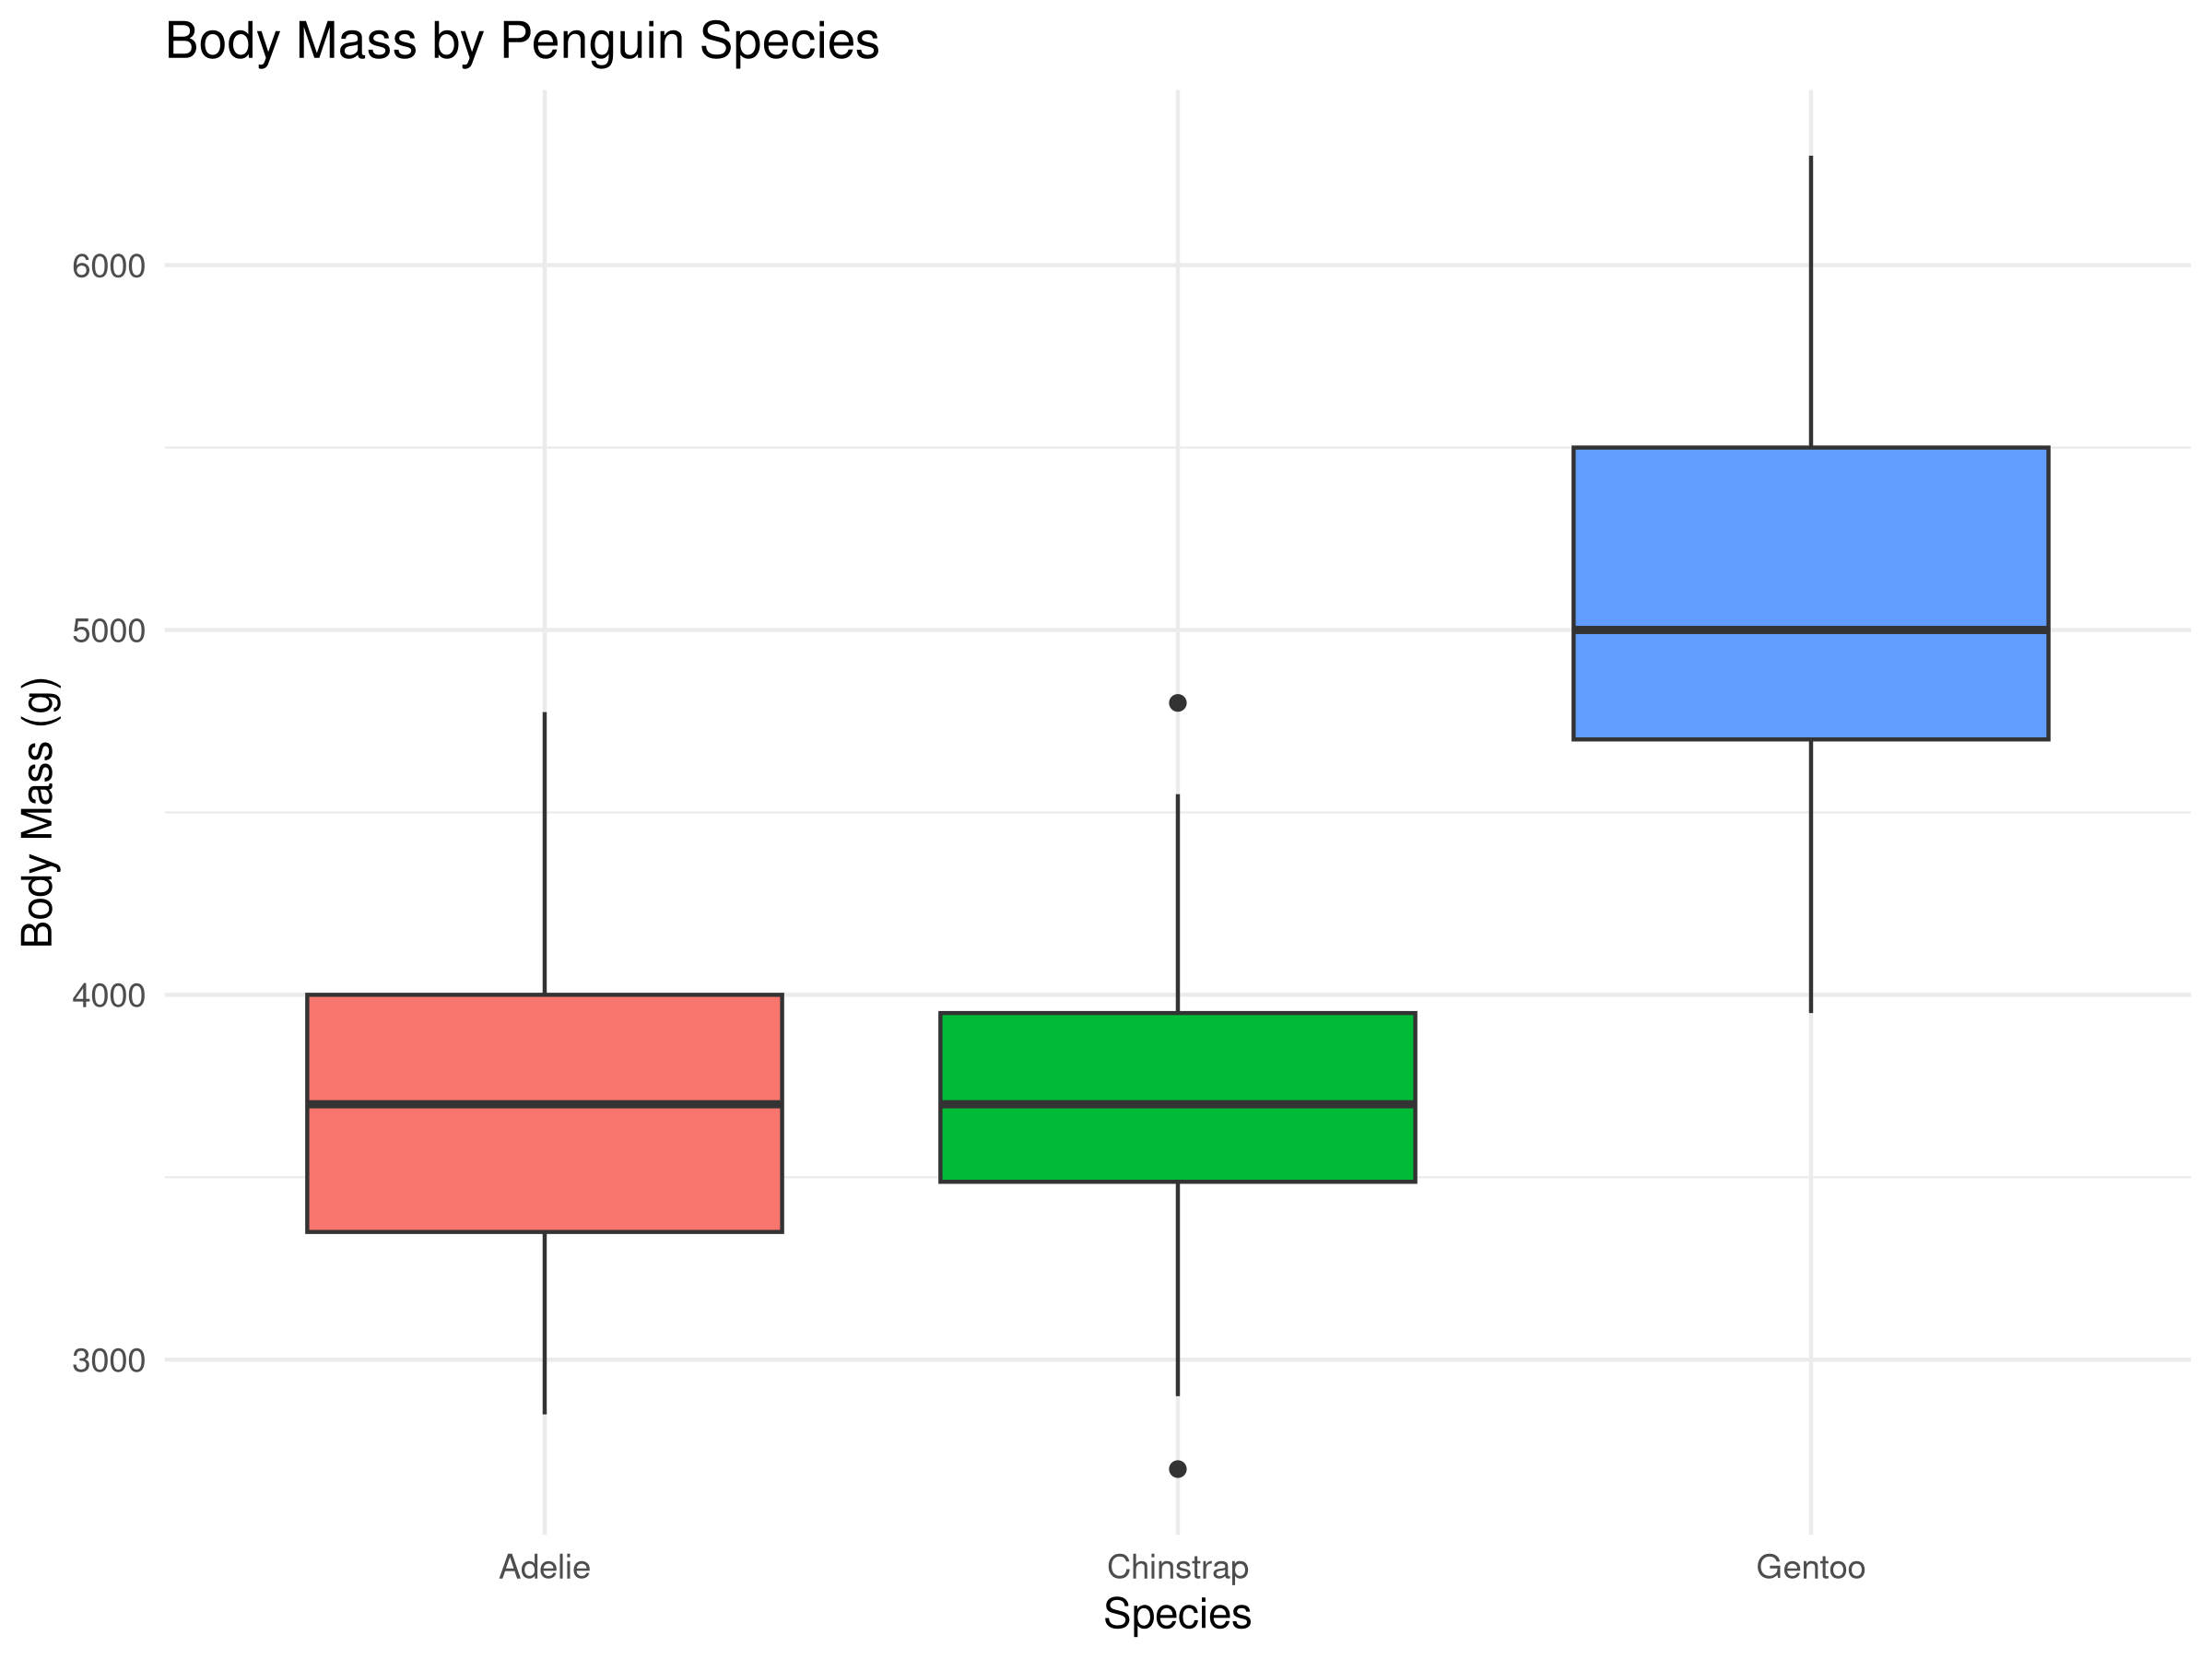
\includegraphics[keepaspectratio]{chapters/02-data-basics_files/figure-pdf/unnamed-chunk-9-2.pdf}}

\begin{Shaded}
\begin{Highlighting}[]
\CommentTok{\# Scatterplot of bill length vs. flipper length}
\FunctionTok{ggplot}\NormalTok{(penguins, }\FunctionTok{aes}\NormalTok{(}\AttributeTok{x =}\NormalTok{ flipper\_length\_mm, }\AttributeTok{y =}\NormalTok{ bill\_length\_mm, }\AttributeTok{color =}\NormalTok{ species)) }\SpecialCharTok{+}
  \FunctionTok{geom\_point}\NormalTok{(}\AttributeTok{alpha =} \FloatTok{0.7}\NormalTok{) }\SpecialCharTok{+}
  \FunctionTok{labs}\NormalTok{(}\AttributeTok{title =} \StringTok{"Bill Length vs. Flipper Length"}\NormalTok{,}
       \AttributeTok{x =} \StringTok{"Flipper Length (mm)"}\NormalTok{,}
       \AttributeTok{y =} \StringTok{"Bill Length (mm)"}\NormalTok{) }\SpecialCharTok{+}
  \FunctionTok{theme\_minimal}\NormalTok{()}
\end{Highlighting}
\end{Shaded}

\pandocbounded{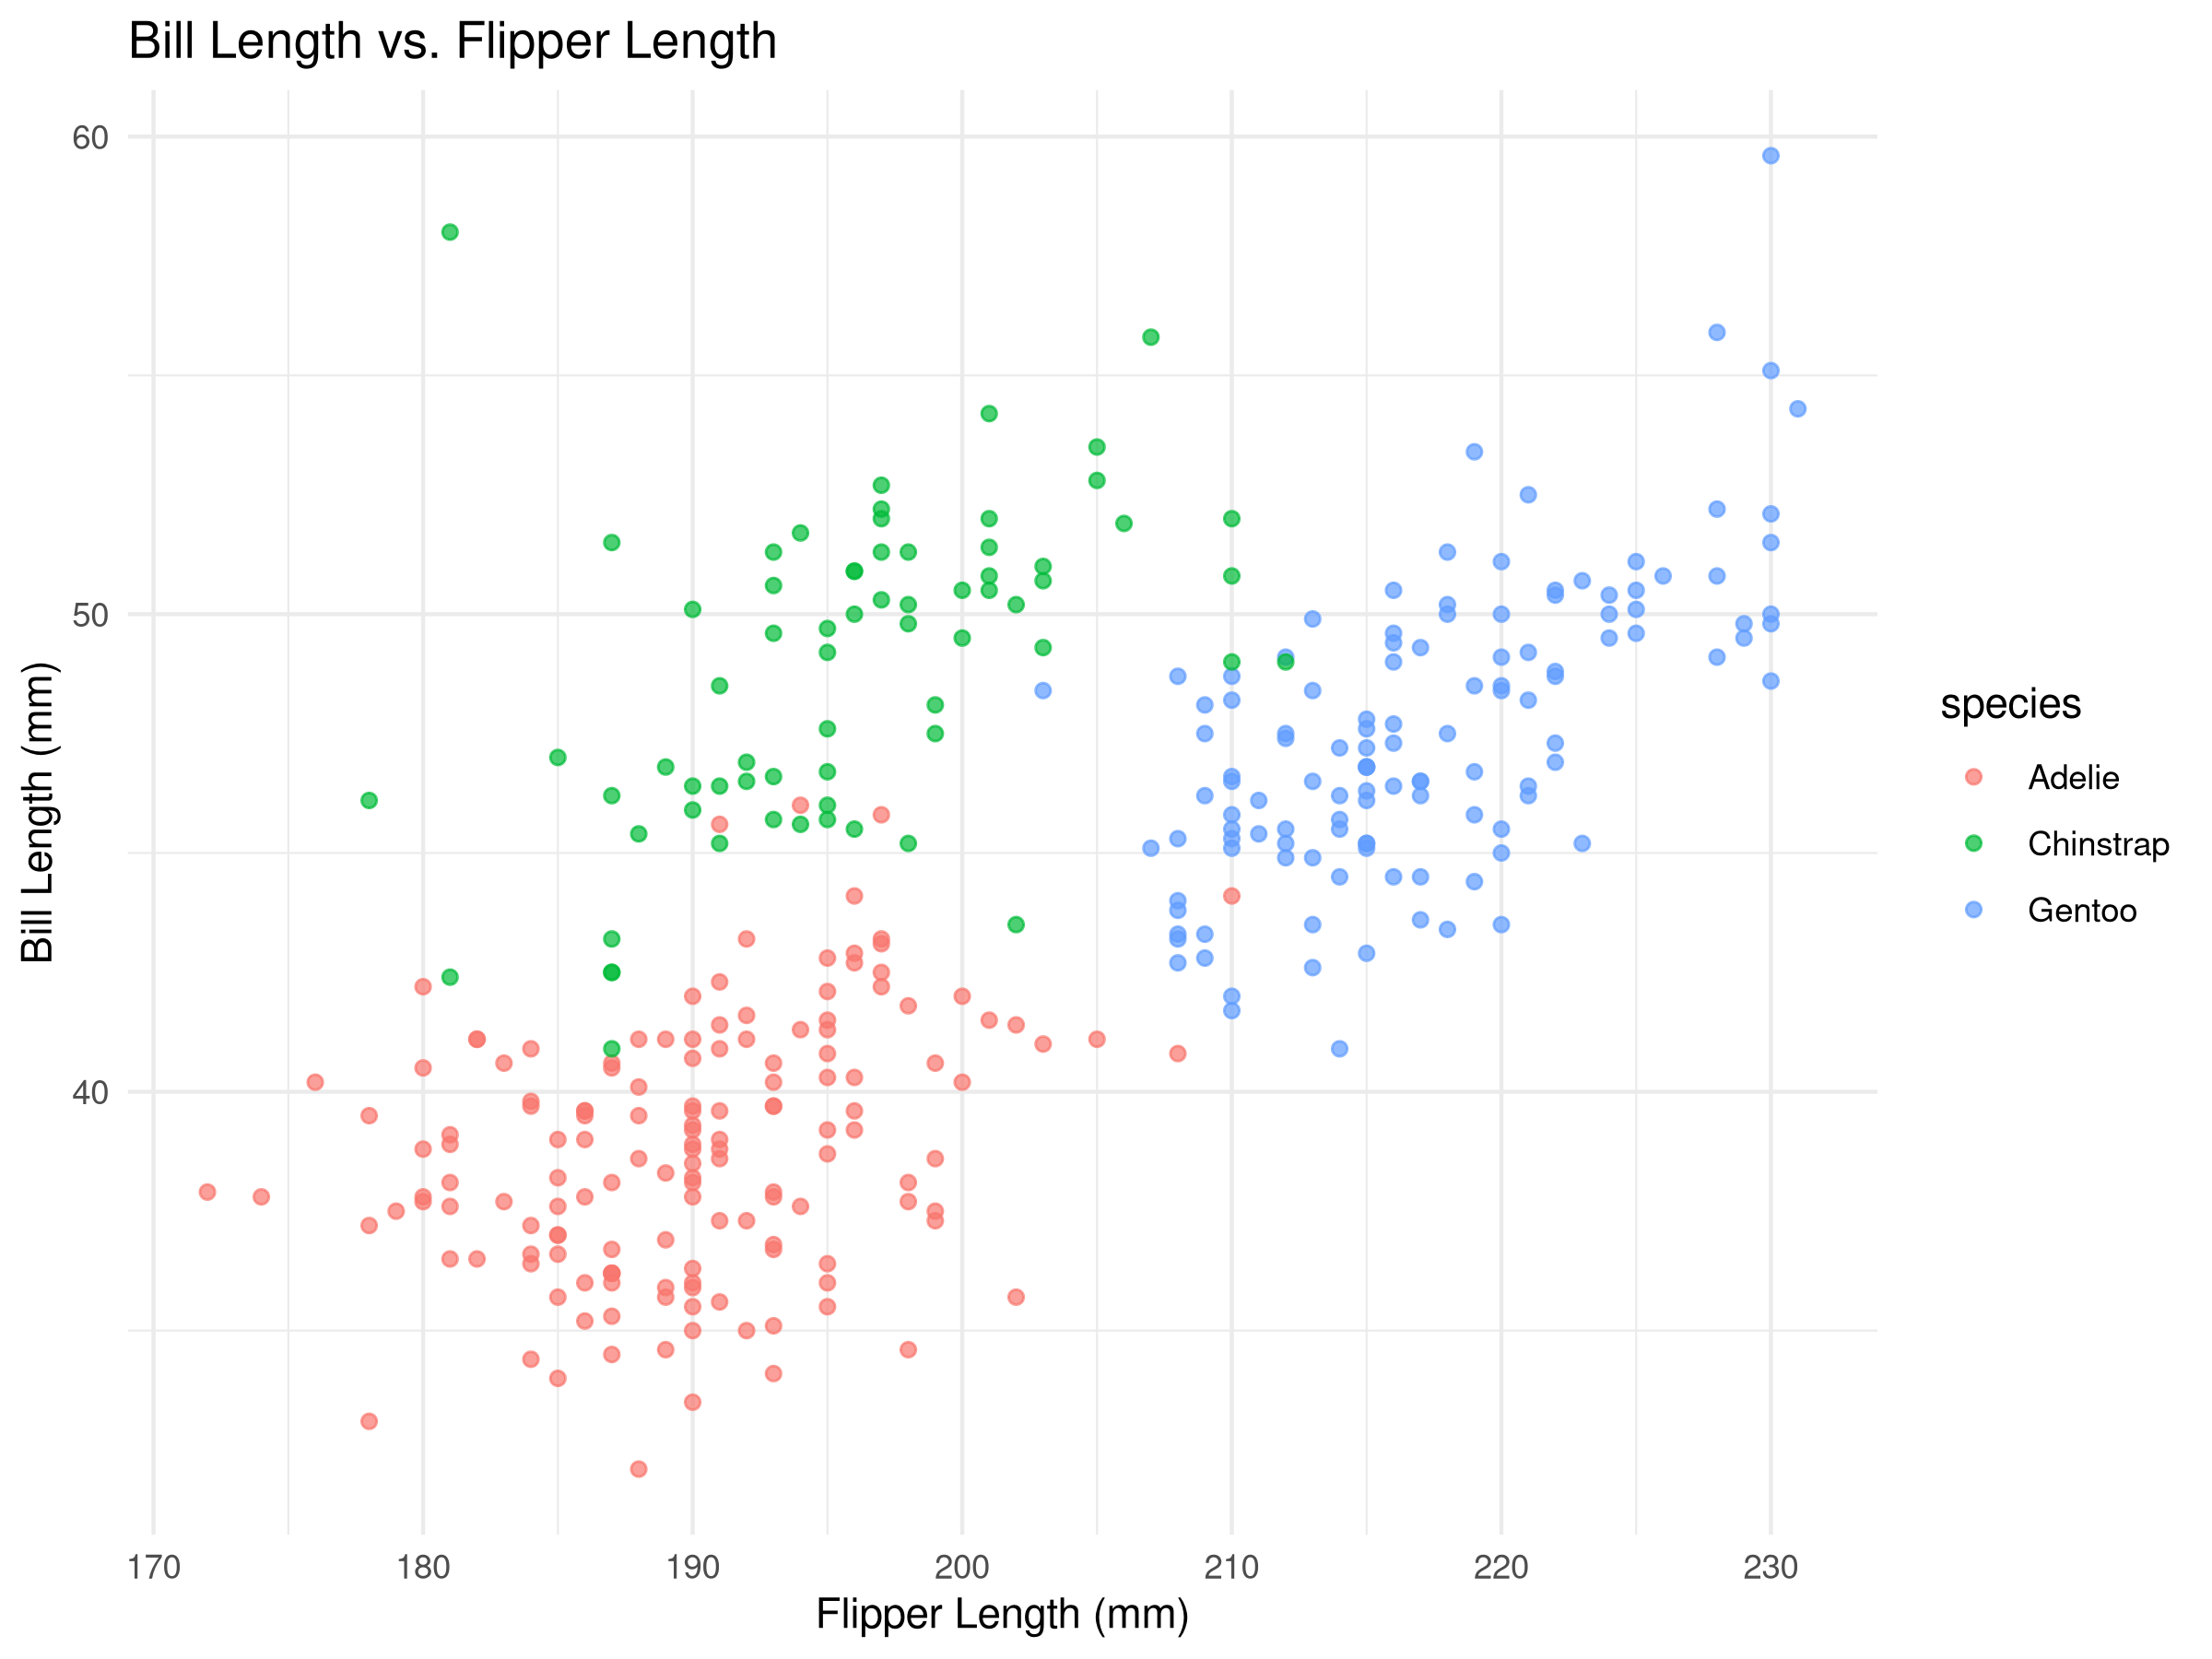
\includegraphics[keepaspectratio]{chapters/02-data-basics_files/figure-pdf/unnamed-chunk-9-3.pdf}}

\section{Summary}\label{summary-1}

In this chapter, we've covered the basics of working with data in R:

\begin{itemize}
\tightlist
\item
  Understanding different data types and structures
\item
  Importing data from various file formats
\item
  Cleaning and preparing data for analysis
\item
  Creating new variables
\item
  Using dplyr for powerful data manipulation
\item
  Conducting initial exploratory data analysis
\end{itemize}

These skills form the foundation for all the analyses we'll perform in
the subsequent chapters. By mastering these basics, you'll be
well-prepared to tackle more complex analytical challenges in various
scientific fields.

\section{Exercises}\label{exercises-1}

\begin{enumerate}
\def\labelenumi{\arabic{enumi}.}
\tightlist
\item
  Load the Palmer Penguins dataset
  (\texttt{../data/environmental/climate\_data.csv}) and create a
  summary of the number of penguins by species and island.
\item
  Calculate the mean and standard deviation of bill length, bill depth,
  and body mass for each penguin species.
\item
  Create a new variable that represents the ratio of flipper length to
  body mass. Interpret what this ratio might represent biologically.
\item
  Create a visualization that shows the relationship between bill length
  and bill depth, colored by species.
\item
  Load the crop yields dataset
  (\texttt{../data/agriculture/crop\_yields.csv}) and analyze trends in
  wheat yields over time for a country of your choice.
\item
  Compare the distributions of body mass between male and female
  penguins using appropriate visualizations.
\end{enumerate}

\part{Data Analysis Fundamentals}

\chapter{Exploratory Data Analysis}\label{exploratory-data-analysis-1}

\section{Introduction}\label{introduction-1}

Exploratory Data Analysis (EDA) is a critical first step in any data
analysis project. In this chapter, you'll learn how to systematically
explore your data to understand its structure, identify patterns, detect
anomalies, and generate hypotheses for further investigation.

\section{The Purpose of Exploratory Data
Analysis}\label{the-purpose-of-exploratory-data-analysis}

Exploratory Data Analysis serves several important purposes in natural
sciences research:

\begin{enumerate}
\def\labelenumi{\arabic{enumi}.}
\tightlist
\item
  \textbf{Understanding Data Structure}: Gain insights into the basic
  properties of your dataset
\item
  \textbf{Checking Data Quality}: Identify missing values, outliers, and
  potential errors
\item
  \textbf{Discovering Patterns}: Detect relationships, trends, and
  distributions
\item
  \textbf{Generating Hypotheses}: Develop questions and hypotheses for
  formal testing
\item
  \textbf{Informing Analysis Choices}: Guide decisions about appropriate
  statistical methods
\end{enumerate}

\section{Summarizing Data}\label{summarizing-data}

\subsection{Descriptive Statistics}\label{descriptive-statistics}

Descriptive statistics provide a concise summary of your data's central
tendency, dispersion, and shape:

\begin{Shaded}
\begin{Highlighting}[]
\CommentTok{\# Load necessary libraries}
\FunctionTok{library}\NormalTok{(tidyverse)}

\CommentTok{\# Load the crop yield dataset}
\NormalTok{crop\_yields }\OtherTok{\textless{}{-}} \FunctionTok{read\_csv}\NormalTok{(}\StringTok{"../data/agriculture/crop\_yields.csv"}\NormalTok{)}

\CommentTok{\# View the first few rows}
\FunctionTok{head}\NormalTok{(crop\_yields)}
\end{Highlighting}
\end{Shaded}

\begin{verbatim}
# A tibble: 6 x 14
  Entity      Code   Year `Wheat (tonnes per hectare)` Rice (tonnes per hectar~1
  <chr>       <chr> <dbl>                        <dbl>                     <dbl>
1 Afghanistan AFG    1961                        1.02                       1.52
2 Afghanistan AFG    1962                        0.974                      1.52
3 Afghanistan AFG    1963                        0.832                      1.52
4 Afghanistan AFG    1964                        0.951                      1.73
5 Afghanistan AFG    1965                        0.972                      1.73
6 Afghanistan AFG    1966                        0.867                      1.52
# i abbreviated name: 1: `Rice (tonnes per hectare)`
# i 9 more variables: `Maize (tonnes per hectare)` <dbl>,
#   `Soybeans (tonnes per hectare)` <dbl>,
#   `Potatoes (tonnes per hectare)` <dbl>, `Beans (tonnes per hectare)` <dbl>,
#   `Peas (tonnes per hectare)` <dbl>, `Cassava (tonnes per hectare)` <dbl>,
#   `Barley (tonnes per hectare)` <dbl>,
#   `Cocoa beans (tonnes per hectare)` <dbl>, ...
\end{verbatim}

\begin{Shaded}
\begin{Highlighting}[]
\CommentTok{\# Get summary statistics for wheat yields}
\NormalTok{wheat\_summary }\OtherTok{\textless{}{-}}\NormalTok{ crop\_yields }\SpecialCharTok{\%\textgreater{}\%}
  \FunctionTok{filter}\NormalTok{(}\SpecialCharTok{!}\FunctionTok{is.na}\NormalTok{(}\StringTok{\textasciigrave{}}\AttributeTok{Wheat (tonnes per hectare)}\StringTok{\textasciigrave{}}\NormalTok{)) }\SpecialCharTok{\%\textgreater{}\%}
  \FunctionTok{summarize}\NormalTok{(}
    \AttributeTok{Mean =} \FunctionTok{mean}\NormalTok{(}\StringTok{\textasciigrave{}}\AttributeTok{Wheat (tonnes per hectare)}\StringTok{\textasciigrave{}}\NormalTok{, }\AttributeTok{na.rm =} \ConstantTok{TRUE}\NormalTok{),}
    \AttributeTok{Median =} \FunctionTok{median}\NormalTok{(}\StringTok{\textasciigrave{}}\AttributeTok{Wheat (tonnes per hectare)}\StringTok{\textasciigrave{}}\NormalTok{, }\AttributeTok{na.rm =} \ConstantTok{TRUE}\NormalTok{),}
    \AttributeTok{StdDev =} \FunctionTok{sd}\NormalTok{(}\StringTok{\textasciigrave{}}\AttributeTok{Wheat (tonnes per hectare)}\StringTok{\textasciigrave{}}\NormalTok{, }\AttributeTok{na.rm =} \ConstantTok{TRUE}\NormalTok{),}
    \AttributeTok{Min =} \FunctionTok{min}\NormalTok{(}\StringTok{\textasciigrave{}}\AttributeTok{Wheat (tonnes per hectare)}\StringTok{\textasciigrave{}}\NormalTok{, }\AttributeTok{na.rm =} \ConstantTok{TRUE}\NormalTok{),}
    \AttributeTok{Max =} \FunctionTok{max}\NormalTok{(}\StringTok{\textasciigrave{}}\AttributeTok{Wheat (tonnes per hectare)}\StringTok{\textasciigrave{}}\NormalTok{, }\AttributeTok{na.rm =} \ConstantTok{TRUE}\NormalTok{),}
    \AttributeTok{Q1 =} \FunctionTok{quantile}\NormalTok{(}\StringTok{\textasciigrave{}}\AttributeTok{Wheat (tonnes per hectare)}\StringTok{\textasciigrave{}}\NormalTok{, }\FloatTok{0.25}\NormalTok{, }\AttributeTok{na.rm =} \ConstantTok{TRUE}\NormalTok{),}
    \AttributeTok{Q3 =} \FunctionTok{quantile}\NormalTok{(}\StringTok{\textasciigrave{}}\AttributeTok{Wheat (tonnes per hectare)}\StringTok{\textasciigrave{}}\NormalTok{, }\FloatTok{0.75}\NormalTok{, }\AttributeTok{na.rm =} \ConstantTok{TRUE}\NormalTok{)}
\NormalTok{  )}

\CommentTok{\# Display the summary statistics}
\NormalTok{knitr}\SpecialCharTok{::}\FunctionTok{kable}\NormalTok{(wheat\_summary, }\AttributeTok{caption =} \StringTok{"Summary Statistics for Global Wheat Yields"}\NormalTok{)}
\end{Highlighting}
\end{Shaded}

\begin{longtable}[]{@{}rrrrrrr@{}}
\caption{Summary Statistics for Global Wheat Yields}\tabularnewline
\toprule\noalign{}
Mean & Median & StdDev & Min & Max & Q1 & Q3 \\
\midrule\noalign{}
\endfirsthead
\toprule\noalign{}
Mean & Median & StdDev & Min & Max & Q1 & Q3 \\
\midrule\noalign{}
\endhead
\bottomrule\noalign{}
\endlastfoot
2.434914 & 1.99 & 1.687949 & 0 & 10.6677 & 1.228 & 3.1245 \\
\end{longtable}

\begin{Shaded}
\begin{Highlighting}[]
\CommentTok{\# Visualize the distribution of wheat yields}
\FunctionTok{ggplot}\NormalTok{(crop\_yields, }\FunctionTok{aes}\NormalTok{(}\AttributeTok{x =} \StringTok{\textasciigrave{}}\AttributeTok{Wheat (tonnes per hectare)}\StringTok{\textasciigrave{}}\NormalTok{)) }\SpecialCharTok{+}
  \FunctionTok{geom\_histogram}\NormalTok{(}\AttributeTok{bins =} \DecValTok{30}\NormalTok{, }\AttributeTok{fill =} \StringTok{"forestgreen"}\NormalTok{, }\AttributeTok{color =} \StringTok{"black"}\NormalTok{, }\AttributeTok{alpha =} \FloatTok{0.7}\NormalTok{) }\SpecialCharTok{+}
  \FunctionTok{labs}\NormalTok{(}\AttributeTok{title =} \StringTok{"Distribution of Global Wheat Yields"}\NormalTok{,}
       \AttributeTok{x =} \StringTok{"Wheat Yield (tonnes per hectare)"}\NormalTok{,}
       \AttributeTok{y =} \StringTok{"Frequency"}\NormalTok{) }\SpecialCharTok{+}
  \FunctionTok{theme\_minimal}\NormalTok{()}
\end{Highlighting}
\end{Shaded}

\pandocbounded{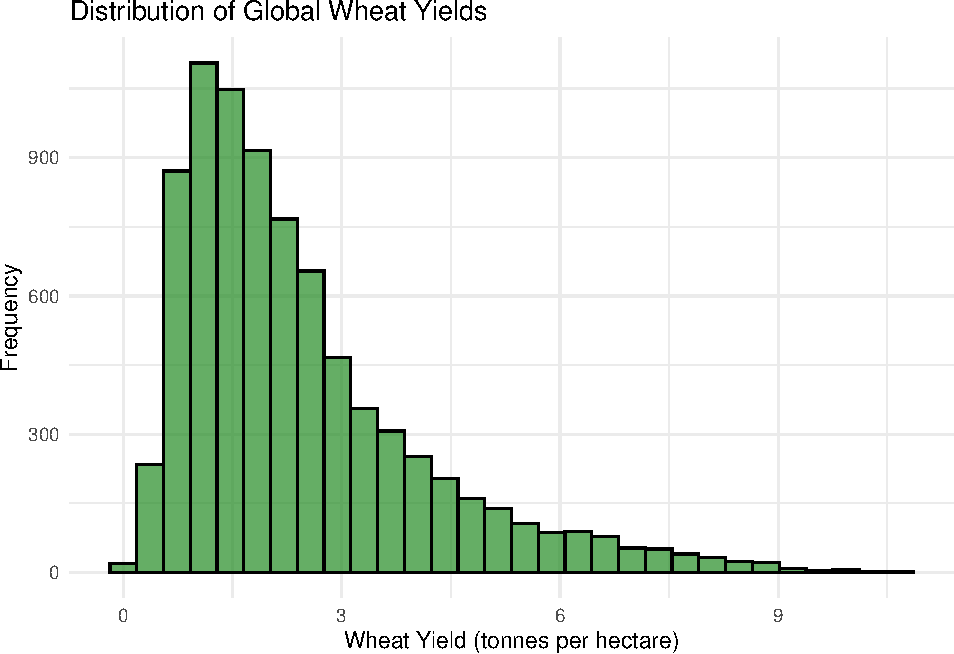
\includegraphics[keepaspectratio]{chapters/03-exploratory-analysis_files/figure-pdf/unnamed-chunk-1-1.pdf}}

\begin{Shaded}
\begin{Highlighting}[]
\CommentTok{\# Identify top wheat{-}producing countries (by average yield)}
\NormalTok{top\_wheat\_countries }\OtherTok{\textless{}{-}}\NormalTok{ crop\_yields }\SpecialCharTok{\%\textgreater{}\%}
  \FunctionTok{filter}\NormalTok{(}\SpecialCharTok{!}\FunctionTok{is.na}\NormalTok{(}\StringTok{\textasciigrave{}}\AttributeTok{Wheat (tonnes per hectare)}\StringTok{\textasciigrave{}}\NormalTok{)) }\SpecialCharTok{\%\textgreater{}\%}
  \FunctionTok{group\_by}\NormalTok{(Entity) }\SpecialCharTok{\%\textgreater{}\%}
  \FunctionTok{summarize}\NormalTok{(}\AttributeTok{Avg\_Yield =} \FunctionTok{mean}\NormalTok{(}\StringTok{\textasciigrave{}}\AttributeTok{Wheat (tonnes per hectare)}\StringTok{\textasciigrave{}}\NormalTok{, }\AttributeTok{na.rm =} \ConstantTok{TRUE}\NormalTok{)) }\SpecialCharTok{\%\textgreater{}\%}
  \FunctionTok{arrange}\NormalTok{(}\FunctionTok{desc}\NormalTok{(Avg\_Yield)) }\SpecialCharTok{\%\textgreater{}\%}
  \FunctionTok{head}\NormalTok{(}\DecValTok{10}\NormalTok{)}

\CommentTok{\# Display the top countries}
\NormalTok{knitr}\SpecialCharTok{::}\FunctionTok{kable}\NormalTok{(top\_wheat\_countries, }\AttributeTok{caption =} \StringTok{"Top 10 Countries by Average Wheat Yield"}\NormalTok{)}
\end{Highlighting}
\end{Shaded}

\begin{longtable}[]{@{}lr@{}}
\caption{Top 10 Countries by Average Wheat Yield}\tabularnewline
\toprule\noalign{}
Entity & Avg\_Yield \\
\midrule\noalign{}
\endfirsthead
\toprule\noalign{}
Entity & Avg\_Yield \\
\midrule\noalign{}
\endhead
\bottomrule\noalign{}
\endlastfoot
Belgium & 8.544200 \\
Netherlands & 7.030172 \\
Ireland & 6.829840 \\
United Kingdom & 6.366400 \\
Denmark & 6.175285 \\
Luxembourg & 5.977411 \\
Germany & 5.893978 \\
Europe, Western & 5.723267 \\
France & 5.645341 \\
Northern Europe & 5.589988 \\
\end{longtable}

\subsection{Frequency Tables}\label{frequency-tables}

Frequency tables are useful for understanding the distribution of
categorical variables:

\begin{Shaded}
\begin{Highlighting}[]
\CommentTok{\# Let\textquotesingle{}s create a categorical variable based on wheat yield levels}
\NormalTok{crop\_yields\_with\_categories }\OtherTok{\textless{}{-}}\NormalTok{ crop\_yields }\SpecialCharTok{\%\textgreater{}\%}
  \FunctionTok{filter}\NormalTok{(}\SpecialCharTok{!}\FunctionTok{is.na}\NormalTok{(}\StringTok{\textasciigrave{}}\AttributeTok{Wheat (tonnes per hectare)}\StringTok{\textasciigrave{}}\NormalTok{)) }\SpecialCharTok{\%\textgreater{}\%}
  \FunctionTok{mutate}\NormalTok{(}\AttributeTok{yield\_category =} \FunctionTok{case\_when}\NormalTok{(}
    \StringTok{\textasciigrave{}}\AttributeTok{Wheat (tonnes per hectare)}\StringTok{\textasciigrave{}} \SpecialCharTok{\textless{}} \DecValTok{2} \SpecialCharTok{\textasciitilde{}} \StringTok{"Low"}\NormalTok{,}
    \StringTok{\textasciigrave{}}\AttributeTok{Wheat (tonnes per hectare)}\StringTok{\textasciigrave{}} \SpecialCharTok{\textgreater{}=} \DecValTok{2} \SpecialCharTok{\&} \StringTok{\textasciigrave{}}\AttributeTok{Wheat (tonnes per hectare)}\StringTok{\textasciigrave{}} \SpecialCharTok{\textless{}} \DecValTok{4} \SpecialCharTok{\textasciitilde{}} \StringTok{"Medium"}\NormalTok{,}
    \StringTok{\textasciigrave{}}\AttributeTok{Wheat (tonnes per hectare)}\StringTok{\textasciigrave{}} \SpecialCharTok{\textgreater{}=} \DecValTok{4} \SpecialCharTok{\textasciitilde{}} \StringTok{"High"}
\NormalTok{  ))}

\CommentTok{\# Frequency table for yield categories}
\FunctionTok{table}\NormalTok{(crop\_yields\_with\_categories}\SpecialCharTok{$}\NormalTok{yield\_category)}
\end{Highlighting}
\end{Shaded}

\begin{verbatim}

  High    Low Medium 
  1279   4081   2741 
\end{verbatim}

\begin{Shaded}
\begin{Highlighting}[]
\CommentTok{\# Proportions}
\FunctionTok{prop.table}\NormalTok{(}\FunctionTok{table}\NormalTok{(crop\_yields\_with\_categories}\SpecialCharTok{$}\NormalTok{yield\_category))}
\end{Highlighting}
\end{Shaded}

\begin{verbatim}

     High       Low    Medium 
0.1578817 0.5037650 0.3383533 
\end{verbatim}

\begin{Shaded}
\begin{Highlighting}[]
\CommentTok{\# Create a decade variable for temporal analysis}
\NormalTok{crop\_yields\_with\_categories }\OtherTok{\textless{}{-}}\NormalTok{ crop\_yields\_with\_categories }\SpecialCharTok{\%\textgreater{}\%}
  \FunctionTok{mutate}\NormalTok{(}\AttributeTok{decade =} \FunctionTok{floor}\NormalTok{(Year }\SpecialCharTok{/} \DecValTok{10}\NormalTok{) }\SpecialCharTok{*} \DecValTok{10}\NormalTok{)}

\CommentTok{\# Two{-}way frequency table: yield category by decade}
\NormalTok{yield\_decade\_table }\OtherTok{\textless{}{-}} \FunctionTok{table}\NormalTok{(crop\_yields\_with\_categories}\SpecialCharTok{$}\NormalTok{yield\_category, }
\NormalTok{                            crop\_yields\_with\_categories}\SpecialCharTok{$}\NormalTok{decade)}
\NormalTok{yield\_decade\_table}
\end{Highlighting}
\end{Shaded}

\begin{verbatim}
        
         1960 1970 1980 1990 2000 2010
  High     34  102  200  261  326  356
  Low     838  833  760  681  563  406
  Medium  239  335  344  550  656  617
\end{verbatim}

\begin{Shaded}
\begin{Highlighting}[]
\CommentTok{\# Convert to proportions (by row)}
\FunctionTok{prop.table}\NormalTok{(yield\_decade\_table, }\AttributeTok{margin =} \DecValTok{1}\NormalTok{)}
\end{Highlighting}
\end{Shaded}

\begin{verbatim}
        
               1960       1970       1980       1990       2000       2010
  High   0.02658327 0.07974980 0.15637217 0.20406568 0.25488663 0.27834246
  Low    0.20534183 0.20411664 0.18622887 0.16687086 0.13795638 0.09948542
  Medium 0.08719445 0.12221817 0.12550164 0.20065669 0.23932871 0.22510033
\end{verbatim}

\section{Visualizing Distributions}\label{visualizing-distributions}

\subsection{Histograms and Density
Plots}\label{histograms-and-density-plots}

Histograms and density plots help visualize the distribution of
continuous variables:

\begin{Shaded}
\begin{Highlighting}[]
\CommentTok{\# Histogram of wheat yields}
\FunctionTok{ggplot}\NormalTok{(crop\_yields, }\FunctionTok{aes}\NormalTok{(}\AttributeTok{x =} \StringTok{\textasciigrave{}}\AttributeTok{Wheat (tonnes per hectare)}\StringTok{\textasciigrave{}}\NormalTok{)) }\SpecialCharTok{+}
  \FunctionTok{geom\_histogram}\NormalTok{(}\AttributeTok{bins =} \DecValTok{30}\NormalTok{, }\AttributeTok{fill =} \StringTok{"darkgreen"}\NormalTok{, }\AttributeTok{color =} \StringTok{"white"}\NormalTok{, }\AttributeTok{na.rm =} \ConstantTok{TRUE}\NormalTok{) }\SpecialCharTok{+}
  \FunctionTok{labs}\NormalTok{(}\AttributeTok{title =} \StringTok{"Histogram of Wheat Yields"}\NormalTok{, }
       \AttributeTok{x =} \StringTok{"Wheat Yield (tonnes per hectare)"}\NormalTok{, }
       \AttributeTok{y =} \StringTok{"Frequency"}\NormalTok{) }\SpecialCharTok{+}
  \FunctionTok{theme\_minimal}\NormalTok{()}
\end{Highlighting}
\end{Shaded}

\pandocbounded{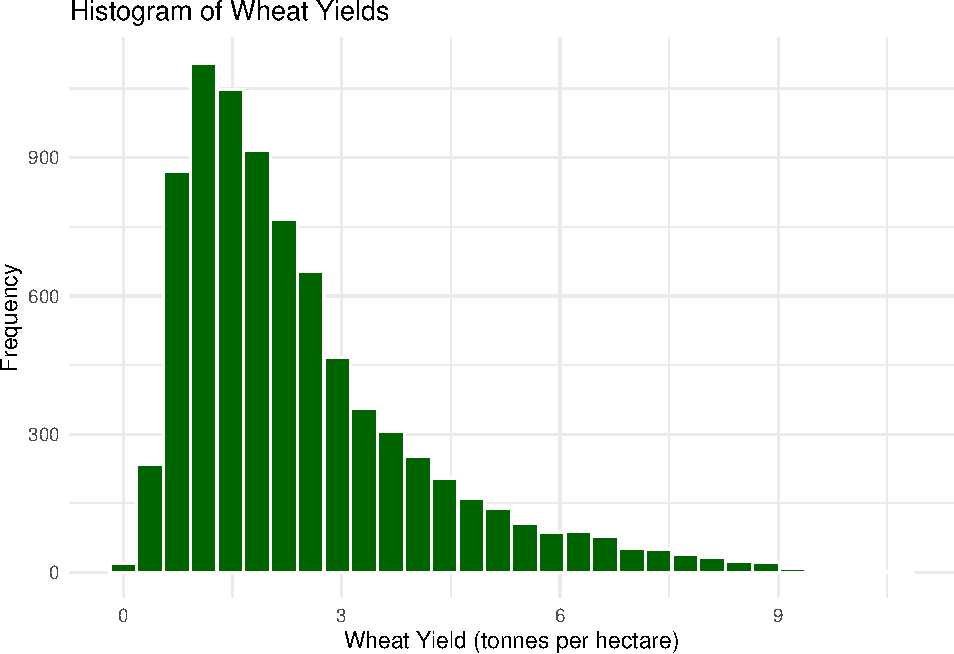
\includegraphics[keepaspectratio]{chapters/03-exploratory-analysis_files/figure-pdf/unnamed-chunk-3-1.pdf}}

\begin{Shaded}
\begin{Highlighting}[]
\CommentTok{\# Density plot}
\FunctionTok{ggplot}\NormalTok{(crop\_yields, }\FunctionTok{aes}\NormalTok{(}\AttributeTok{x =} \StringTok{\textasciigrave{}}\AttributeTok{Wheat (tonnes per hectare)}\StringTok{\textasciigrave{}}\NormalTok{)) }\SpecialCharTok{+}
  \FunctionTok{geom\_density}\NormalTok{(}\AttributeTok{fill =} \StringTok{"darkgreen"}\NormalTok{, }\AttributeTok{alpha =} \FloatTok{0.5}\NormalTok{, }\AttributeTok{na.rm =} \ConstantTok{TRUE}\NormalTok{) }\SpecialCharTok{+}
  \FunctionTok{labs}\NormalTok{(}\AttributeTok{title =} \StringTok{"Density Plot of Wheat Yields"}\NormalTok{, }
       \AttributeTok{x =} \StringTok{"Wheat Yield (tonnes per hectare)"}\NormalTok{, }
       \AttributeTok{y =} \StringTok{"Density"}\NormalTok{) }\SpecialCharTok{+}
  \FunctionTok{theme\_minimal}\NormalTok{()}
\end{Highlighting}
\end{Shaded}

\pandocbounded{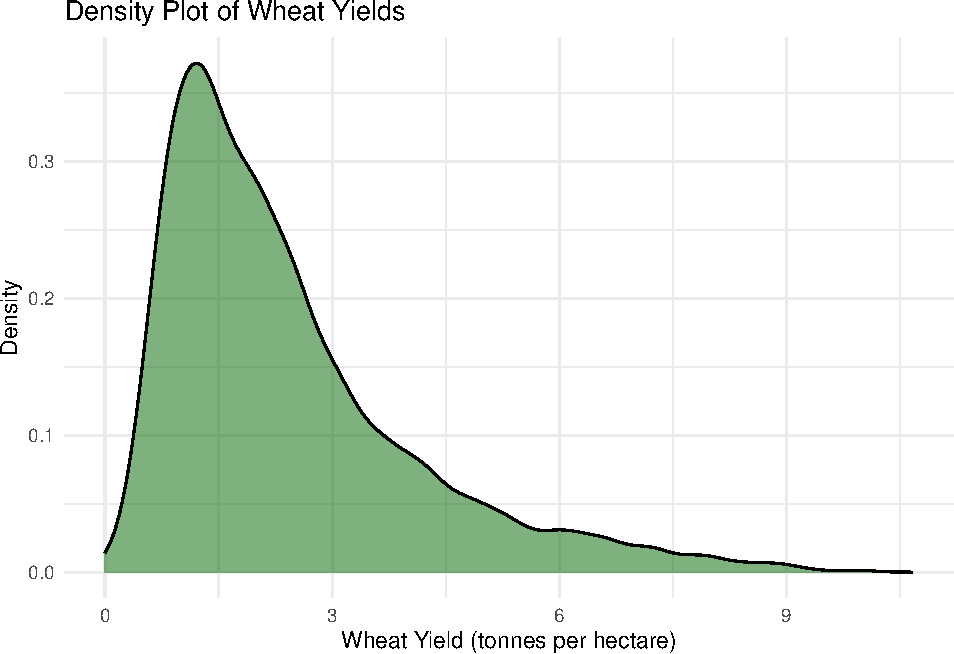
\includegraphics[keepaspectratio]{chapters/03-exploratory-analysis_files/figure-pdf/unnamed-chunk-3-2.pdf}}

\begin{Shaded}
\begin{Highlighting}[]
\CommentTok{\# Histogram with density overlay}
\FunctionTok{ggplot}\NormalTok{(crop\_yields, }\FunctionTok{aes}\NormalTok{(}\AttributeTok{x =} \StringTok{\textasciigrave{}}\AttributeTok{Wheat (tonnes per hectare)}\StringTok{\textasciigrave{}}\NormalTok{)) }\SpecialCharTok{+}
  \FunctionTok{geom\_histogram}\NormalTok{(}\FunctionTok{aes}\NormalTok{(}\AttributeTok{y =}\NormalTok{ ..density..), }\AttributeTok{bins =} \DecValTok{30}\NormalTok{, }\AttributeTok{fill =} \StringTok{"darkgreen"}\NormalTok{, }\AttributeTok{color =} \StringTok{"white"}\NormalTok{, }\AttributeTok{na.rm =} \ConstantTok{TRUE}\NormalTok{) }\SpecialCharTok{+}
  \FunctionTok{geom\_density}\NormalTok{(}\AttributeTok{color =} \StringTok{"darkgreen"}\NormalTok{, }\AttributeTok{linewidth =} \DecValTok{1}\NormalTok{, }\AttributeTok{na.rm =} \ConstantTok{TRUE}\NormalTok{) }\SpecialCharTok{+}
  \FunctionTok{labs}\NormalTok{(}\AttributeTok{title =} \StringTok{"Distribution of Wheat Yields"}\NormalTok{, }
       \AttributeTok{x =} \StringTok{"Wheat Yield (tonnes per hectare)"}\NormalTok{, }
       \AttributeTok{y =} \StringTok{"Density"}\NormalTok{) }\SpecialCharTok{+}
  \FunctionTok{theme\_minimal}\NormalTok{()}
\end{Highlighting}
\end{Shaded}

\pandocbounded{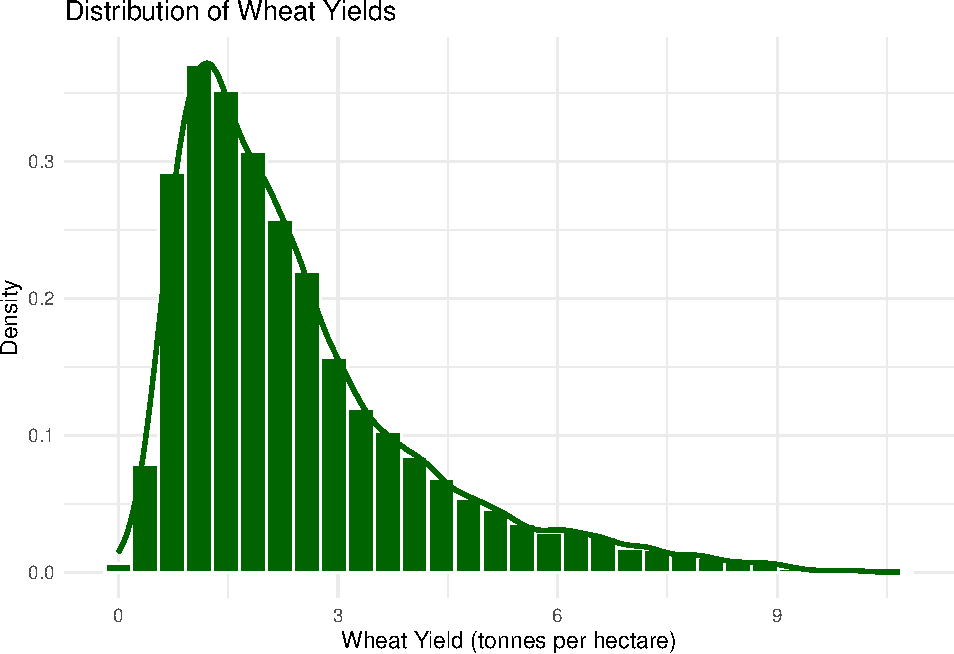
\includegraphics[keepaspectratio]{chapters/03-exploratory-analysis_files/figure-pdf/unnamed-chunk-3-3.pdf}}

\subsection{Box Plots}\label{box-plots}

Box plots are excellent for comparing distributions across groups:

\begin{Shaded}
\begin{Highlighting}[]
\CommentTok{\# Select a few major countries for comparison}
\NormalTok{major\_wheat\_producers }\OtherTok{\textless{}{-}} \FunctionTok{c}\NormalTok{(}\StringTok{"United States"}\NormalTok{, }\StringTok{"China"}\NormalTok{, }\StringTok{"India"}\NormalTok{, }\StringTok{"Russia"}\NormalTok{, }\StringTok{"France"}\NormalTok{, }\StringTok{"Australia"}\NormalTok{)}

\CommentTok{\# Filter data for these countries and recent years}
\NormalTok{recent\_wheat\_data }\OtherTok{\textless{}{-}}\NormalTok{ crop\_yields }\SpecialCharTok{\%\textgreater{}\%}
  \FunctionTok{filter}\NormalTok{(Entity }\SpecialCharTok{\%in\%}\NormalTok{ major\_wheat\_producers, }
\NormalTok{         Year }\SpecialCharTok{\textgreater{}=} \DecValTok{2000}\NormalTok{,}
         \SpecialCharTok{!}\FunctionTok{is.na}\NormalTok{(}\StringTok{\textasciigrave{}}\AttributeTok{Wheat (tonnes per hectare)}\StringTok{\textasciigrave{}}\NormalTok{))}

\CommentTok{\# Box plot of wheat yields by country}
\FunctionTok{ggplot}\NormalTok{(recent\_wheat\_data, }\FunctionTok{aes}\NormalTok{(}\AttributeTok{x =}\NormalTok{ Entity, }\AttributeTok{y =} \StringTok{\textasciigrave{}}\AttributeTok{Wheat (tonnes per hectare)}\StringTok{\textasciigrave{}}\NormalTok{)) }\SpecialCharTok{+}
  \FunctionTok{geom\_boxplot}\NormalTok{(}\AttributeTok{fill =} \StringTok{"darkgreen"}\NormalTok{, }\AttributeTok{alpha =} \FloatTok{0.7}\NormalTok{) }\SpecialCharTok{+}
  \FunctionTok{labs}\NormalTok{(}\AttributeTok{title =} \StringTok{"Wheat Yields by Country (2000{-}present)"}\NormalTok{, }
       \AttributeTok{x =} \StringTok{"Country"}\NormalTok{, }
       \AttributeTok{y =} \StringTok{"Wheat Yield (tonnes per hectare)"}\NormalTok{) }\SpecialCharTok{+}
  \FunctionTok{theme\_minimal}\NormalTok{() }\SpecialCharTok{+}
  \FunctionTok{theme}\NormalTok{(}\AttributeTok{axis.text.x =} \FunctionTok{element\_text}\NormalTok{(}\AttributeTok{angle =} \DecValTok{45}\NormalTok{, }\AttributeTok{hjust =} \DecValTok{1}\NormalTok{))}
\end{Highlighting}
\end{Shaded}

\pandocbounded{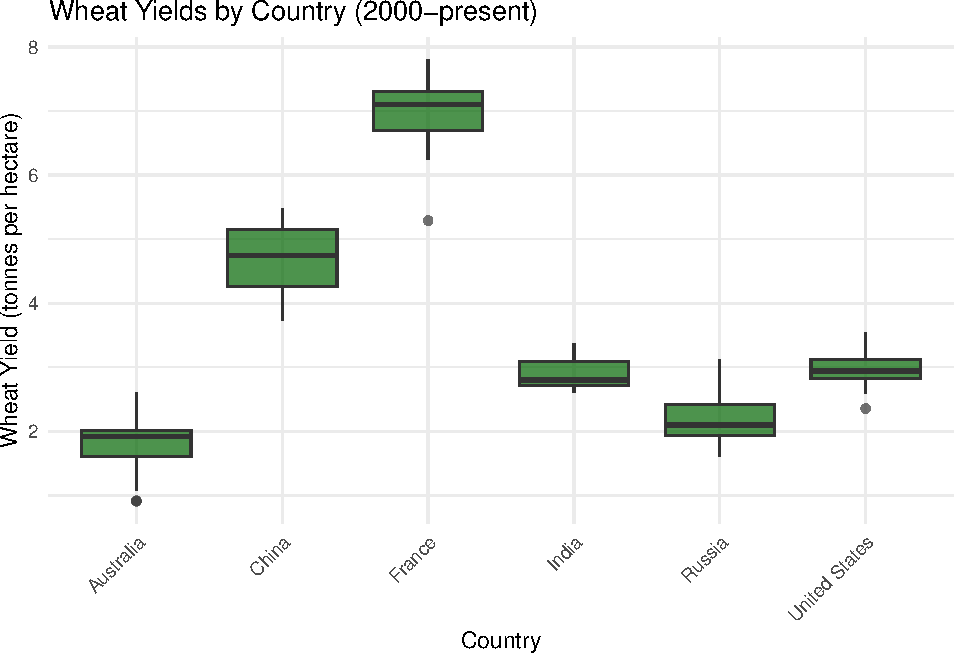
\includegraphics[keepaspectratio]{chapters/03-exploratory-analysis_files/figure-pdf/unnamed-chunk-4-1.pdf}}

\begin{Shaded}
\begin{Highlighting}[]
\CommentTok{\# Enhanced box plot with jittered points}
\FunctionTok{ggplot}\NormalTok{(recent\_wheat\_data, }\FunctionTok{aes}\NormalTok{(}\AttributeTok{x =}\NormalTok{ Entity, }\AttributeTok{y =} \StringTok{\textasciigrave{}}\AttributeTok{Wheat (tonnes per hectare)}\StringTok{\textasciigrave{}}\NormalTok{)) }\SpecialCharTok{+}
  \FunctionTok{geom\_boxplot}\NormalTok{(}\AttributeTok{fill =} \StringTok{"darkgreen"}\NormalTok{, }\AttributeTok{alpha =} \FloatTok{0.5}\NormalTok{) }\SpecialCharTok{+}
  \FunctionTok{geom\_jitter}\NormalTok{(}\AttributeTok{width =} \FloatTok{0.2}\NormalTok{, }\AttributeTok{alpha =} \FloatTok{0.5}\NormalTok{, }\AttributeTok{color =} \StringTok{"darkgreen"}\NormalTok{) }\SpecialCharTok{+}
  \FunctionTok{labs}\NormalTok{(}\AttributeTok{title =} \StringTok{"Wheat Yields by Country (2000{-}present)"}\NormalTok{, }
       \AttributeTok{x =} \StringTok{"Country"}\NormalTok{, }
       \AttributeTok{y =} \StringTok{"Wheat Yield (tonnes per hectare)"}\NormalTok{) }\SpecialCharTok{+}
  \FunctionTok{theme\_minimal}\NormalTok{() }\SpecialCharTok{+}
  \FunctionTok{theme}\NormalTok{(}\AttributeTok{axis.text.x =} \FunctionTok{element\_text}\NormalTok{(}\AttributeTok{angle =} \DecValTok{45}\NormalTok{, }\AttributeTok{hjust =} \DecValTok{1}\NormalTok{))}
\end{Highlighting}
\end{Shaded}

\pandocbounded{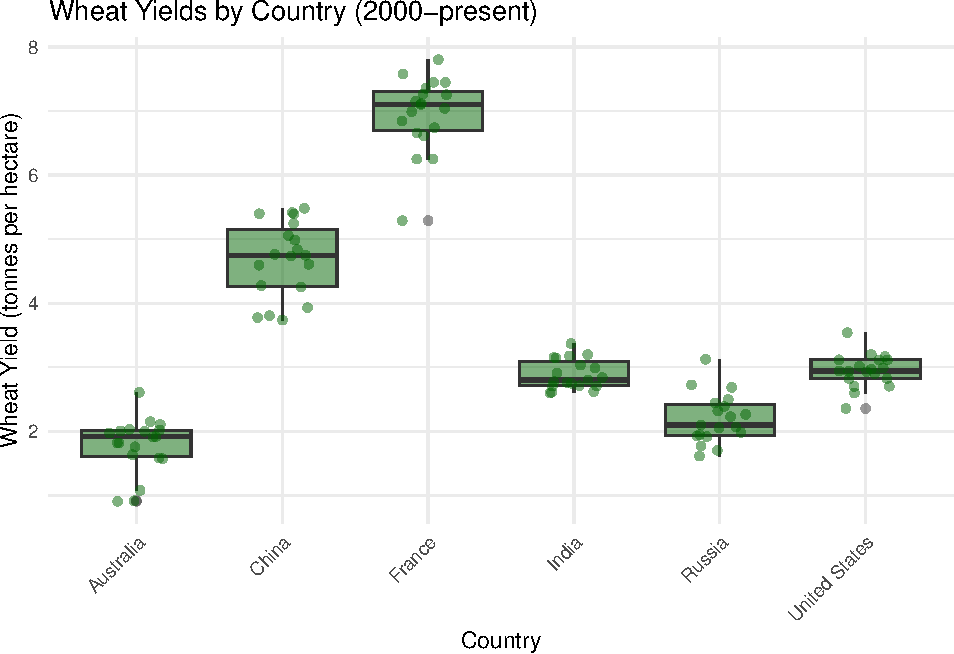
\includegraphics[keepaspectratio]{chapters/03-exploratory-analysis_files/figure-pdf/unnamed-chunk-4-2.pdf}}

\subsection{Bar Charts}\label{bar-charts}

Bar charts are useful for visualizing categorical data:

\begin{Shaded}
\begin{Highlighting}[]
\CommentTok{\# Calculate average wheat yield by country for the last decade}
\NormalTok{recent\_avg\_yields }\OtherTok{\textless{}{-}}\NormalTok{ crop\_yields }\SpecialCharTok{\%\textgreater{}\%}
  \FunctionTok{filter}\NormalTok{(Year }\SpecialCharTok{\textgreater{}=} \DecValTok{2010}\NormalTok{, }\SpecialCharTok{!}\FunctionTok{is.na}\NormalTok{(}\StringTok{\textasciigrave{}}\AttributeTok{Wheat (tonnes per hectare)}\StringTok{\textasciigrave{}}\NormalTok{)) }\SpecialCharTok{\%\textgreater{}\%}
  \FunctionTok{group\_by}\NormalTok{(Entity) }\SpecialCharTok{\%\textgreater{}\%}
  \FunctionTok{summarize}\NormalTok{(}\AttributeTok{avg\_wheat\_yield =} \FunctionTok{mean}\NormalTok{(}\StringTok{\textasciigrave{}}\AttributeTok{Wheat (tonnes per hectare)}\StringTok{\textasciigrave{}}\NormalTok{, }\AttributeTok{na.rm =} \ConstantTok{TRUE}\NormalTok{)) }\SpecialCharTok{\%\textgreater{}\%}
  \FunctionTok{arrange}\NormalTok{(}\FunctionTok{desc}\NormalTok{(avg\_wheat\_yield)) }\SpecialCharTok{\%\textgreater{}\%}
  \FunctionTok{head}\NormalTok{(}\DecValTok{10}\NormalTok{)  }\CommentTok{\# Top 10 countries}

\CommentTok{\# Bar chart of average wheat yields}
\FunctionTok{ggplot}\NormalTok{(recent\_avg\_yields, }\FunctionTok{aes}\NormalTok{(}\AttributeTok{x =} \FunctionTok{reorder}\NormalTok{(Entity, avg\_wheat\_yield), }\AttributeTok{y =}\NormalTok{ avg\_wheat\_yield)) }\SpecialCharTok{+}
  \FunctionTok{geom\_bar}\NormalTok{(}\AttributeTok{stat =} \StringTok{"identity"}\NormalTok{, }\AttributeTok{fill =} \StringTok{"darkgreen"}\NormalTok{) }\SpecialCharTok{+}
  \FunctionTok{labs}\NormalTok{(}\AttributeTok{title =} \StringTok{"Top 10 Countries by Average Wheat Yield (2010{-}present)"}\NormalTok{, }
       \AttributeTok{x =} \StringTok{"Country"}\NormalTok{, }
       \AttributeTok{y =} \StringTok{"Average Wheat Yield (tonnes per hectare)"}\NormalTok{) }\SpecialCharTok{+}
  \FunctionTok{theme\_minimal}\NormalTok{() }\SpecialCharTok{+}
  \FunctionTok{theme}\NormalTok{(}\AttributeTok{axis.text.x =} \FunctionTok{element\_text}\NormalTok{(}\AttributeTok{angle =} \DecValTok{45}\NormalTok{, }\AttributeTok{hjust =} \DecValTok{1}\NormalTok{))}
\end{Highlighting}
\end{Shaded}

\pandocbounded{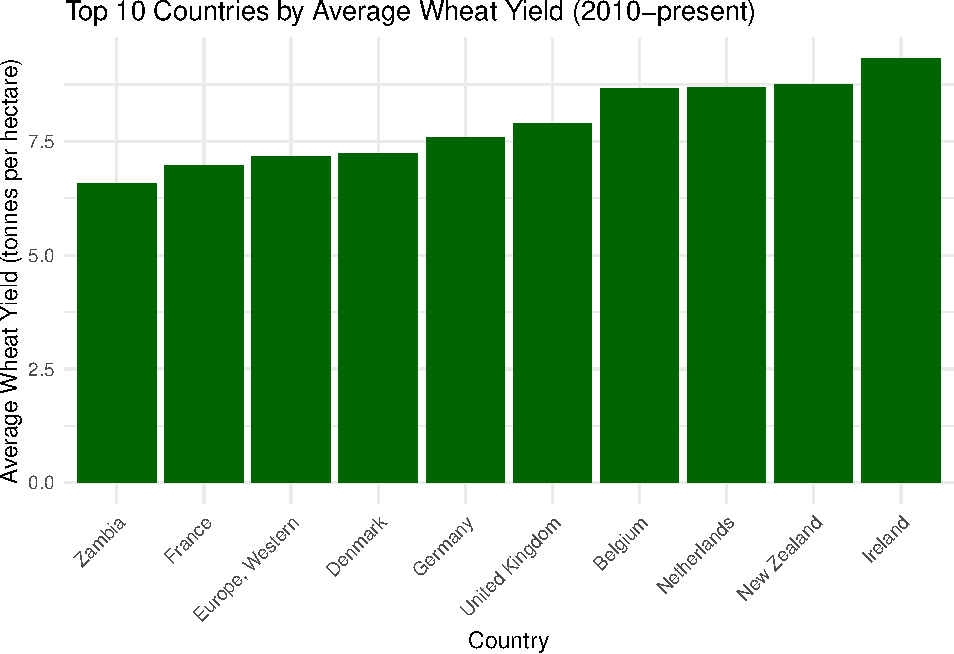
\includegraphics[keepaspectratio]{chapters/03-exploratory-analysis_files/figure-pdf/unnamed-chunk-5-1.pdf}}

\section{Exploring Relationships}\label{exploring-relationships}

\subsection{Scatter Plots}\label{scatter-plots}

Scatter plots help visualize relationships between two continuous
variables:

\begin{Shaded}
\begin{Highlighting}[]
\CommentTok{\# Let\textquotesingle{}s compare wheat and rice yields}
\NormalTok{crop\_yields\_filtered }\OtherTok{\textless{}{-}}\NormalTok{ crop\_yields }\SpecialCharTok{\%\textgreater{}\%}
  \FunctionTok{filter}\NormalTok{(}\SpecialCharTok{!}\FunctionTok{is.na}\NormalTok{(}\StringTok{\textasciigrave{}}\AttributeTok{Wheat (tonnes per hectare)}\StringTok{\textasciigrave{}}\NormalTok{), }\SpecialCharTok{!}\FunctionTok{is.na}\NormalTok{(}\StringTok{\textasciigrave{}}\AttributeTok{Rice (tonnes per hectare)}\StringTok{\textasciigrave{}}\NormalTok{)) }\SpecialCharTok{\%\textgreater{}\%}
  \FunctionTok{filter}\NormalTok{(Year }\SpecialCharTok{\textgreater{}=} \DecValTok{2000}\NormalTok{)}

\CommentTok{\# Basic scatter plot}
\FunctionTok{ggplot}\NormalTok{(crop\_yields\_filtered, }\FunctionTok{aes}\NormalTok{(}\AttributeTok{x =} \StringTok{\textasciigrave{}}\AttributeTok{Wheat (tonnes per hectare)}\StringTok{\textasciigrave{}}\NormalTok{, }\AttributeTok{y =} \StringTok{\textasciigrave{}}\AttributeTok{Rice (tonnes per hectare)}\StringTok{\textasciigrave{}}\NormalTok{)) }\SpecialCharTok{+}
  \FunctionTok{geom\_point}\NormalTok{(}\AttributeTok{alpha =} \FloatTok{0.5}\NormalTok{, }\AttributeTok{color =} \StringTok{"darkgreen"}\NormalTok{) }\SpecialCharTok{+}
  \FunctionTok{labs}\NormalTok{(}\AttributeTok{title =} \StringTok{"Relationship between Wheat and Rice Yields"}\NormalTok{,}
       \AttributeTok{x =} \StringTok{"Wheat Yield (tonnes per hectare)"}\NormalTok{, }
       \AttributeTok{y =} \StringTok{"Rice Yield (tonnes per hectare)"}\NormalTok{) }\SpecialCharTok{+}
  \FunctionTok{theme\_minimal}\NormalTok{()}
\end{Highlighting}
\end{Shaded}

\pandocbounded{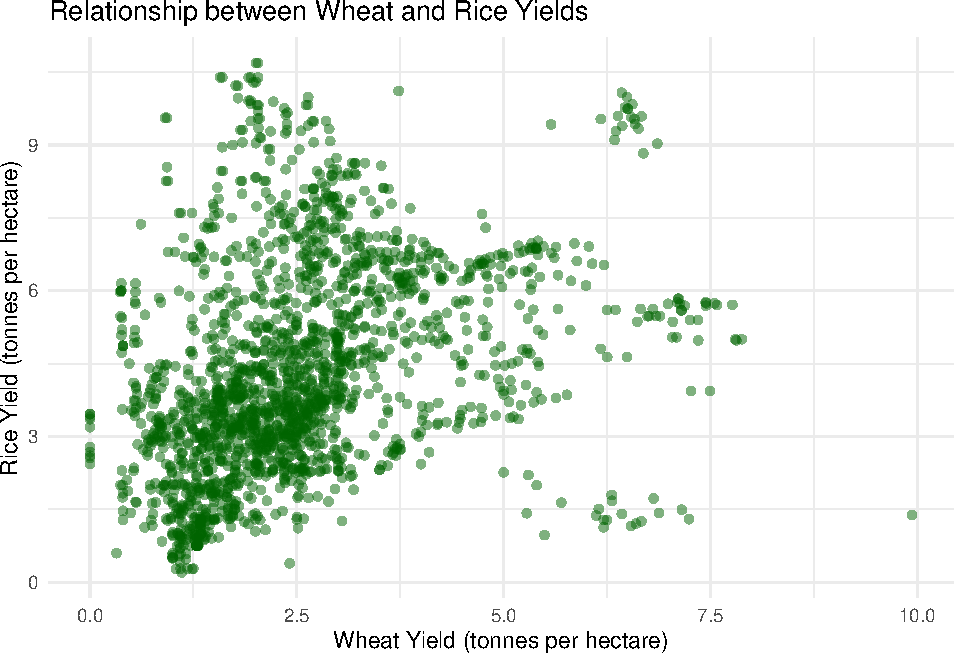
\includegraphics[keepaspectratio]{chapters/03-exploratory-analysis_files/figure-pdf/unnamed-chunk-6-1.pdf}}

\begin{Shaded}
\begin{Highlighting}[]
\CommentTok{\# Scatter plot with color by continent (we\textquotesingle{}ll need to add continent information)}
\CommentTok{\# For demonstration, let\textquotesingle{}s create a simple mapping for a few countries}
\NormalTok{continent\_mapping }\OtherTok{\textless{}{-}} \FunctionTok{tibble}\NormalTok{(}
  \AttributeTok{Entity =} \FunctionTok{c}\NormalTok{(}\StringTok{"United States"}\NormalTok{, }\StringTok{"Canada"}\NormalTok{, }\StringTok{"Mexico"}\NormalTok{, }
             \StringTok{"China"}\NormalTok{, }\StringTok{"India"}\NormalTok{, }\StringTok{"Japan"}\NormalTok{, }
             \StringTok{"Germany"}\NormalTok{, }\StringTok{"France"}\NormalTok{, }\StringTok{"United Kingdom"}\NormalTok{, }
             \StringTok{"Brazil"}\NormalTok{, }\StringTok{"Argentina"}\NormalTok{, }\StringTok{"Chile"}\NormalTok{,}
             \StringTok{"Egypt"}\NormalTok{, }\StringTok{"Nigeria"}\NormalTok{, }\StringTok{"South Africa"}\NormalTok{,}
             \StringTok{"Australia"}\NormalTok{, }\StringTok{"New Zealand"}\NormalTok{),}
  \AttributeTok{Continent =} \FunctionTok{c}\NormalTok{(}\FunctionTok{rep}\NormalTok{(}\StringTok{"North America"}\NormalTok{, }\DecValTok{3}\NormalTok{), }
                \FunctionTok{rep}\NormalTok{(}\StringTok{"Asia"}\NormalTok{, }\DecValTok{3}\NormalTok{), }
                \FunctionTok{rep}\NormalTok{(}\StringTok{"Europe"}\NormalTok{, }\DecValTok{3}\NormalTok{), }
                \FunctionTok{rep}\NormalTok{(}\StringTok{"South America"}\NormalTok{, }\DecValTok{3}\NormalTok{),}
                \FunctionTok{rep}\NormalTok{(}\StringTok{"Africa"}\NormalTok{, }\DecValTok{3}\NormalTok{),}
                \FunctionTok{rep}\NormalTok{(}\StringTok{"Oceania"}\NormalTok{, }\DecValTok{2}\NormalTok{))}
\NormalTok{)}

\CommentTok{\# Join with our dataset}
\NormalTok{crop\_yields\_with\_continent }\OtherTok{\textless{}{-}}\NormalTok{ crop\_yields\_filtered }\SpecialCharTok{\%\textgreater{}\%}
  \FunctionTok{inner\_join}\NormalTok{(continent\_mapping, }\AttributeTok{by =} \StringTok{"Entity"}\NormalTok{)}

\CommentTok{\# Scatter plot with color by continent}
\FunctionTok{ggplot}\NormalTok{(crop\_yields\_with\_continent, }\FunctionTok{aes}\NormalTok{(}\AttributeTok{x =} \StringTok{\textasciigrave{}}\AttributeTok{Wheat (tonnes per hectare)}\StringTok{\textasciigrave{}}\NormalTok{, }\AttributeTok{y =} \StringTok{\textasciigrave{}}\AttributeTok{Rice (tonnes per hectare)}\StringTok{\textasciigrave{}}\NormalTok{, }\AttributeTok{color =}\NormalTok{ Continent)) }\SpecialCharTok{+}
  \FunctionTok{geom\_point}\NormalTok{(}\AttributeTok{size =} \DecValTok{3}\NormalTok{, }\AttributeTok{alpha =} \FloatTok{0.7}\NormalTok{) }\SpecialCharTok{+}
  \FunctionTok{labs}\NormalTok{(}\AttributeTok{title =} \StringTok{"Relationship between Wheat and Rice Yields by Continent"}\NormalTok{,}
       \AttributeTok{x =} \StringTok{"Wheat Yield (tonnes per hectare)"}\NormalTok{, }
       \AttributeTok{y =} \StringTok{"Rice Yield (tonnes per hectare)"}\NormalTok{) }\SpecialCharTok{+}
  \FunctionTok{theme\_minimal}\NormalTok{()}
\end{Highlighting}
\end{Shaded}

\pandocbounded{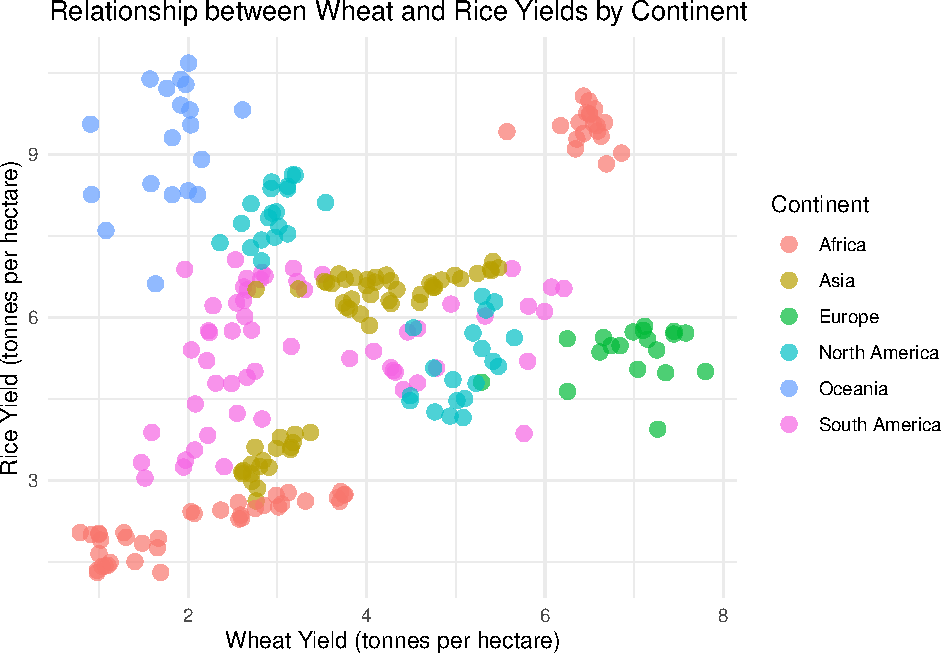
\includegraphics[keepaspectratio]{chapters/03-exploratory-analysis_files/figure-pdf/unnamed-chunk-6-2.pdf}}

\subsection{Correlation Analysis}\label{correlation-analysis}

Correlation analysis quantifies the strength and direction of
relationships between variables:

\begin{Shaded}
\begin{Highlighting}[]
\CommentTok{\# Select numeric columns for correlation analysis}
\NormalTok{crop\_numeric }\OtherTok{\textless{}{-}}\NormalTok{ crop\_yields }\SpecialCharTok{\%\textgreater{}\%}
  \FunctionTok{select}\NormalTok{(}\StringTok{\textasciigrave{}}\AttributeTok{Wheat (tonnes per hectare)}\StringTok{\textasciigrave{}}\NormalTok{, }\StringTok{\textasciigrave{}}\AttributeTok{Rice (tonnes per hectare)}\StringTok{\textasciigrave{}}\NormalTok{, }\StringTok{\textasciigrave{}}\AttributeTok{Maize (tonnes per hectare)}\StringTok{\textasciigrave{}}\NormalTok{, }\StringTok{\textasciigrave{}}\AttributeTok{Soybeans (tonnes per hectare)}\StringTok{\textasciigrave{}}\NormalTok{, }\StringTok{\textasciigrave{}}\AttributeTok{Potatoes (tonnes per hectare)}\StringTok{\textasciigrave{}}\NormalTok{, }\StringTok{\textasciigrave{}}\AttributeTok{Beans (tonnes per hectare)}\StringTok{\textasciigrave{}}\NormalTok{) }\SpecialCharTok{\%\textgreater{}\%}
  \FunctionTok{na.omit}\NormalTok{()}

\CommentTok{\# Correlation matrix}
\NormalTok{cor\_matrix }\OtherTok{\textless{}{-}} \FunctionTok{cor}\NormalTok{(crop\_numeric)}
\FunctionTok{round}\NormalTok{(cor\_matrix, }\DecValTok{2}\NormalTok{)}
\end{Highlighting}
\end{Shaded}

\begin{verbatim}
                              Wheat (tonnes per hectare)
Wheat (tonnes per hectare)                          1.00
Rice (tonnes per hectare)                           0.43
Maize (tonnes per hectare)                          0.57
Soybeans (tonnes per hectare)                       0.47
Potatoes (tonnes per hectare)                       0.57
Beans (tonnes per hectare)                          0.44
                              Rice (tonnes per hectare)
Wheat (tonnes per hectare)                         0.43
Rice (tonnes per hectare)                          1.00
Maize (tonnes per hectare)                         0.73
Soybeans (tonnes per hectare)                      0.58
Potatoes (tonnes per hectare)                      0.67
Beans (tonnes per hectare)                         0.46
                              Maize (tonnes per hectare)
Wheat (tonnes per hectare)                          0.57
Rice (tonnes per hectare)                           0.73
Maize (tonnes per hectare)                          1.00
Soybeans (tonnes per hectare)                       0.65
Potatoes (tonnes per hectare)                       0.74
Beans (tonnes per hectare)                          0.63
                              Soybeans (tonnes per hectare)
Wheat (tonnes per hectare)                             0.47
Rice (tonnes per hectare)                              0.58
Maize (tonnes per hectare)                             0.65
Soybeans (tonnes per hectare)                          1.00
Potatoes (tonnes per hectare)                          0.59
Beans (tonnes per hectare)                             0.41
                              Potatoes (tonnes per hectare)
Wheat (tonnes per hectare)                             0.57
Rice (tonnes per hectare)                              0.67
Maize (tonnes per hectare)                             0.74
Soybeans (tonnes per hectare)                          0.59
Potatoes (tonnes per hectare)                          1.00
Beans (tonnes per hectare)                             0.46
                              Beans (tonnes per hectare)
Wheat (tonnes per hectare)                          0.44
Rice (tonnes per hectare)                           0.46
Maize (tonnes per hectare)                          0.63
Soybeans (tonnes per hectare)                       0.41
Potatoes (tonnes per hectare)                       0.46
Beans (tonnes per hectare)                          1.00
\end{verbatim}

\begin{Shaded}
\begin{Highlighting}[]
\CommentTok{\# Visualize correlation matrix}
\FunctionTok{library}\NormalTok{(corrplot)}
\FunctionTok{corrplot}\NormalTok{(cor\_matrix, }\AttributeTok{method =} \StringTok{"circle"}\NormalTok{, }\AttributeTok{type =} \StringTok{"upper"}\NormalTok{, }
         \AttributeTok{tl.col =} \StringTok{"black"}\NormalTok{, }\AttributeTok{tl.srt =} \DecValTok{45}\NormalTok{,}
         \AttributeTok{title =} \StringTok{"Correlation Matrix of Crop Yields"}\NormalTok{)}
\end{Highlighting}
\end{Shaded}

\pandocbounded{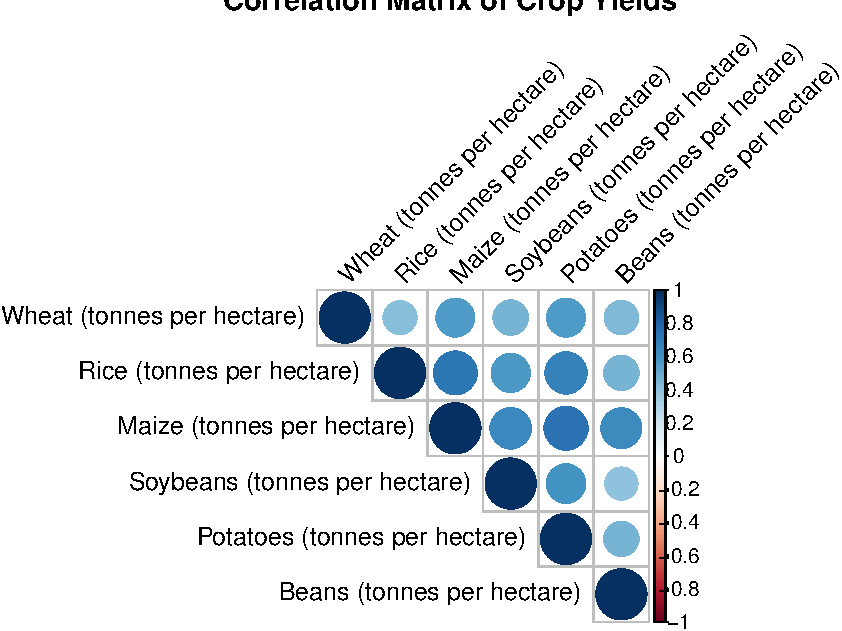
\includegraphics[keepaspectratio]{chapters/03-exploratory-analysis_files/figure-pdf/unnamed-chunk-7-1.pdf}}

\subsection{Pair Plots}\label{pair-plots}

Pair plots provide a comprehensive view of relationships between
multiple variables:

\begin{Shaded}
\begin{Highlighting}[]
\CommentTok{\# Basic pair plot}
\FunctionTok{pairs}\NormalTok{(crop\_numeric, }\AttributeTok{pch =} \DecValTok{19}\NormalTok{, }\AttributeTok{col =} \StringTok{"darkgreen"}\NormalTok{)}
\end{Highlighting}
\end{Shaded}

\pandocbounded{\includegraphics[keepaspectratio]{chapters/03-exploratory-analysis_files/figure-pdf/unnamed-chunk-8-1.pdf}}

\begin{Shaded}
\begin{Highlighting}[]
\CommentTok{\# Enhanced pair plot with GGally}
\FunctionTok{library}\NormalTok{(GGally)}
\FunctionTok{ggpairs}\NormalTok{(crop\_numeric) }\SpecialCharTok{+}
  \FunctionTok{theme\_minimal}\NormalTok{() }\SpecialCharTok{+}
  \FunctionTok{labs}\NormalTok{(}\AttributeTok{title =} \StringTok{"Relationships Between Different Crop Yields"}\NormalTok{)}
\end{Highlighting}
\end{Shaded}

\pandocbounded{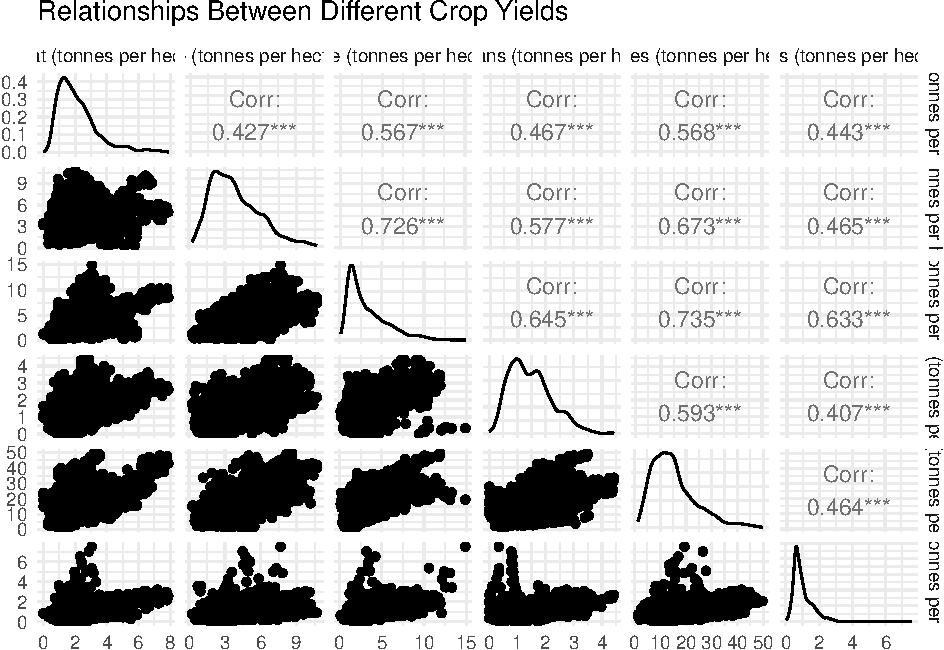
\includegraphics[keepaspectratio]{chapters/03-exploratory-analysis_files/figure-pdf/unnamed-chunk-8-2.pdf}}

\section{Identifying Outliers and
Anomalies}\label{identifying-outliers-and-anomalies}

\subsection{Box Plots for Outlier
Detection}\label{box-plots-for-outlier-detection}

Box plots can help identify potential outliers:

\begin{Shaded}
\begin{Highlighting}[]
\CommentTok{\# Box plot to identify outliers in wheat yield}
\FunctionTok{ggplot}\NormalTok{(crop\_yields, }\FunctionTok{aes}\NormalTok{(}\AttributeTok{y =} \StringTok{\textasciigrave{}}\AttributeTok{Wheat (tonnes per hectare)}\StringTok{\textasciigrave{}}\NormalTok{)) }\SpecialCharTok{+}
  \FunctionTok{geom\_boxplot}\NormalTok{(}\AttributeTok{fill =} \StringTok{"darkgreen"}\NormalTok{, }\AttributeTok{alpha =} \FloatTok{0.7}\NormalTok{, }\AttributeTok{na.rm =} \ConstantTok{TRUE}\NormalTok{) }\SpecialCharTok{+}
  \FunctionTok{labs}\NormalTok{(}\AttributeTok{title =} \StringTok{"Box Plot of Wheat Yields with Potential Outliers"}\NormalTok{,}
       \AttributeTok{y =} \StringTok{"Wheat Yield (tonnes per hectare)"}\NormalTok{) }\SpecialCharTok{+}
  \FunctionTok{theme\_minimal}\NormalTok{()}
\end{Highlighting}
\end{Shaded}

\pandocbounded{\includegraphics[keepaspectratio]{chapters/03-exploratory-analysis_files/figure-pdf/unnamed-chunk-9-1.pdf}}

\begin{Shaded}
\begin{Highlighting}[]
\CommentTok{\# Identify potential outliers}
\NormalTok{wheat\_outliers }\OtherTok{\textless{}{-}}\NormalTok{ crop\_yields }\SpecialCharTok{\%\textgreater{}\%}
  \FunctionTok{filter}\NormalTok{(}\SpecialCharTok{!}\FunctionTok{is.na}\NormalTok{(}\StringTok{\textasciigrave{}}\AttributeTok{Wheat (tonnes per hectare)}\StringTok{\textasciigrave{}}\NormalTok{)) }\SpecialCharTok{\%\textgreater{}\%}
  \FunctionTok{mutate}\NormalTok{(}
    \AttributeTok{q1 =} \FunctionTok{quantile}\NormalTok{(}\StringTok{\textasciigrave{}}\AttributeTok{Wheat (tonnes per hectare)}\StringTok{\textasciigrave{}}\NormalTok{, }\FloatTok{0.25}\NormalTok{),}
    \AttributeTok{q3 =} \FunctionTok{quantile}\NormalTok{(}\StringTok{\textasciigrave{}}\AttributeTok{Wheat (tonnes per hectare)}\StringTok{\textasciigrave{}}\NormalTok{, }\FloatTok{0.75}\NormalTok{),}
    \AttributeTok{iqr =}\NormalTok{ q3 }\SpecialCharTok{{-}}\NormalTok{ q1,}
    \AttributeTok{lower\_bound =}\NormalTok{ q1 }\SpecialCharTok{{-}} \FloatTok{1.5} \SpecialCharTok{*}\NormalTok{ iqr,}
    \AttributeTok{upper\_bound =}\NormalTok{ q3 }\SpecialCharTok{+} \FloatTok{1.5} \SpecialCharTok{*}\NormalTok{ iqr,}
    \AttributeTok{is\_outlier =} \StringTok{\textasciigrave{}}\AttributeTok{Wheat (tonnes per hectare)}\StringTok{\textasciigrave{}} \SpecialCharTok{\textless{}}\NormalTok{ lower\_bound }\SpecialCharTok{|} \StringTok{\textasciigrave{}}\AttributeTok{Wheat (tonnes per hectare)}\StringTok{\textasciigrave{}} \SpecialCharTok{\textgreater{}}\NormalTok{ upper\_bound}
\NormalTok{  ) }\SpecialCharTok{\%\textgreater{}\%}
  \FunctionTok{filter}\NormalTok{(is\_outlier) }\SpecialCharTok{\%\textgreater{}\%}
  \FunctionTok{select}\NormalTok{(Entity, Year, }\StringTok{\textasciigrave{}}\AttributeTok{Wheat (tonnes per hectare)}\StringTok{\textasciigrave{}}\NormalTok{)}

\CommentTok{\# Display the outliers}
\FunctionTok{head}\NormalTok{(wheat\_outliers, }\DecValTok{10}\NormalTok{)}
\end{Highlighting}
\end{Shaded}

\begin{verbatim}
# A tibble: 10 x 3
   Entity   Year `Wheat (tonnes per hectare)`
   <chr>   <dbl>                        <dbl>
 1 Austria  2016                         6.25
 2 Belgium  2000                         7.92
 3 Belgium  2001                         8.05
 4 Belgium  2002                         8.28
 5 Belgium  2003                         8.58
 6 Belgium  2004                         8.98
 7 Belgium  2005                         8.27
 8 Belgium  2006                         8.25
 9 Belgium  2007                         7.89
10 Belgium  2008                         8.76
\end{verbatim}

\subsection{Z-Scores for Outlier
Detection}\label{z-scores-for-outlier-detection}

Z-scores can also help identify outliers:

\begin{Shaded}
\begin{Highlighting}[]
\CommentTok{\# Calculate z{-}scores for wheat yields}
\NormalTok{wheat\_z\_scores }\OtherTok{\textless{}{-}}\NormalTok{ crop\_yields }\SpecialCharTok{\%\textgreater{}\%}
  \FunctionTok{filter}\NormalTok{(}\SpecialCharTok{!}\FunctionTok{is.na}\NormalTok{(}\StringTok{\textasciigrave{}}\AttributeTok{Wheat (tonnes per hectare)}\StringTok{\textasciigrave{}}\NormalTok{)) }\SpecialCharTok{\%\textgreater{}\%}
  \FunctionTok{mutate}\NormalTok{(}
    \AttributeTok{wheat\_mean =} \FunctionTok{mean}\NormalTok{(}\StringTok{\textasciigrave{}}\AttributeTok{Wheat (tonnes per hectare)}\StringTok{\textasciigrave{}}\NormalTok{),}
    \AttributeTok{wheat\_sd =} \FunctionTok{sd}\NormalTok{(}\StringTok{\textasciigrave{}}\AttributeTok{Wheat (tonnes per hectare)}\StringTok{\textasciigrave{}}\NormalTok{),}
    \AttributeTok{z\_score =}\NormalTok{ (}\StringTok{\textasciigrave{}}\AttributeTok{Wheat (tonnes per hectare)}\StringTok{\textasciigrave{}} \SpecialCharTok{{-}}\NormalTok{ wheat\_mean) }\SpecialCharTok{/}\NormalTok{ wheat\_sd,}
    \AttributeTok{is\_extreme =} \FunctionTok{abs}\NormalTok{(z\_score) }\SpecialCharTok{\textgreater{}} \DecValTok{3}
\NormalTok{  )}

\CommentTok{\# Display extreme values (z{-}score \textgreater{} 3 or \textless{} {-}3)}
\NormalTok{wheat\_extremes }\OtherTok{\textless{}{-}}\NormalTok{ wheat\_z\_scores }\SpecialCharTok{\%\textgreater{}\%}
  \FunctionTok{filter}\NormalTok{(is\_extreme) }\SpecialCharTok{\%\textgreater{}\%}
  \FunctionTok{select}\NormalTok{(Entity, Year, }\StringTok{\textasciigrave{}}\AttributeTok{Wheat (tonnes per hectare)}\StringTok{\textasciigrave{}}\NormalTok{, z\_score) }\SpecialCharTok{\%\textgreater{}\%}
  \FunctionTok{arrange}\NormalTok{(}\FunctionTok{desc}\NormalTok{(}\FunctionTok{abs}\NormalTok{(z\_score)))}

\FunctionTok{head}\NormalTok{(wheat\_extremes, }\DecValTok{10}\NormalTok{)}
\end{Highlighting}
\end{Shaded}

\begin{verbatim}
# A tibble: 10 x 4
   Entity       Year `Wheat (tonnes per hectare)` z_score
   <chr>       <dbl>                        <dbl>   <dbl>
 1 Ireland      2015                        10.7     4.88
 2 Ireland      2017                        10.2     4.58
 3 Belgium      2015                        10.0     4.49
 4 Ireland      2014                        10.0     4.49
 5 Zambia       2008                         9.94    4.45
 6 Ireland      2004                         9.92    4.44
 7 New Zealand  2017                         9.86    4.40
 8 Ireland      2011                         9.86    4.40
 9 Ireland      2016                         9.54    4.21
10 Belgium      2009                         9.47    4.16
\end{verbatim}

\section{Time Series Exploration}\label{time-series-exploration}

Agricultural data often contains important temporal patterns:

\begin{Shaded}
\begin{Highlighting}[]
\CommentTok{\# Select a few countries for time series analysis}
\NormalTok{countries\_for\_ts }\OtherTok{\textless{}{-}} \FunctionTok{c}\NormalTok{(}\StringTok{"United States"}\NormalTok{, }\StringTok{"China"}\NormalTok{, }\StringTok{"India"}\NormalTok{, }\StringTok{"France"}\NormalTok{)}

\CommentTok{\# Filter data for these countries}
\NormalTok{wheat\_ts\_data }\OtherTok{\textless{}{-}}\NormalTok{ crop\_yields }\SpecialCharTok{\%\textgreater{}\%}
  \FunctionTok{filter}\NormalTok{(Entity }\SpecialCharTok{\%in\%}\NormalTok{ countries\_for\_ts, }\SpecialCharTok{!}\FunctionTok{is.na}\NormalTok{(}\StringTok{\textasciigrave{}}\AttributeTok{Wheat (tonnes per hectare)}\StringTok{\textasciigrave{}}\NormalTok{)) }\SpecialCharTok{\%\textgreater{}\%}
  \FunctionTok{filter}\NormalTok{(Year }\SpecialCharTok{\textgreater{}=} \DecValTok{1960}\NormalTok{)}

\CommentTok{\# Time series plot}
\FunctionTok{ggplot}\NormalTok{(wheat\_ts\_data, }\FunctionTok{aes}\NormalTok{(}\AttributeTok{x =}\NormalTok{ Year, }\AttributeTok{y =} \StringTok{\textasciigrave{}}\AttributeTok{Wheat (tonnes per hectare)}\StringTok{\textasciigrave{}}\NormalTok{, }\AttributeTok{color =}\NormalTok{ Entity)) }\SpecialCharTok{+}
  \FunctionTok{geom\_line}\NormalTok{(}\AttributeTok{linewidth =} \DecValTok{1}\NormalTok{) }\SpecialCharTok{+}
  \FunctionTok{geom\_point}\NormalTok{(}\AttributeTok{size =} \DecValTok{2}\NormalTok{) }\SpecialCharTok{+}
  \FunctionTok{labs}\NormalTok{(}\AttributeTok{title =} \StringTok{"Wheat Yield Trends Over Time"}\NormalTok{,}
       \AttributeTok{x =} \StringTok{"Year"}\NormalTok{,}
       \AttributeTok{y =} \StringTok{"Wheat Yield (tonnes per hectare)"}\NormalTok{) }\SpecialCharTok{+}
  \FunctionTok{theme\_minimal}\NormalTok{() }\SpecialCharTok{+}
  \FunctionTok{scale\_color\_brewer}\NormalTok{(}\AttributeTok{palette =} \StringTok{"Dark2"}\NormalTok{)}
\end{Highlighting}
\end{Shaded}

\pandocbounded{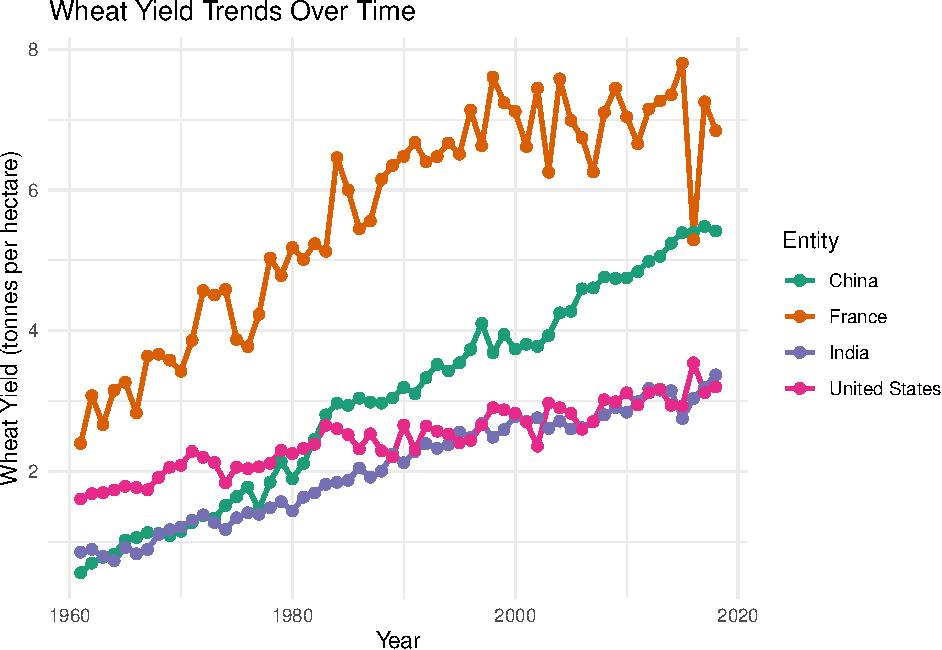
\includegraphics[keepaspectratio]{chapters/03-exploratory-analysis_files/figure-pdf/unnamed-chunk-11-1.pdf}}

\section{Missing Data Analysis}\label{missing-data-analysis}

Understanding patterns of missing data is crucial:

\begin{Shaded}
\begin{Highlighting}[]
\CommentTok{\# Check for missing values in each column}
\FunctionTok{colSums}\NormalTok{(}\FunctionTok{is.na}\NormalTok{(crop\_yields))}
\end{Highlighting}
\end{Shaded}

\begin{verbatim}
                          Entity                             Code 
                               0                             1919 
                            Year       Wheat (tonnes per hectare) 
                               0                             4974 
       Rice (tonnes per hectare)       Maize (tonnes per hectare) 
                            4604                             2301 
   Soybeans (tonnes per hectare)    Potatoes (tonnes per hectare) 
                            7114                             3059 
      Beans (tonnes per hectare)        Peas (tonnes per hectare) 
                            5066                             6840 
    Cassava (tonnes per hectare)      Barley (tonnes per hectare) 
                            5887                             6342 
Cocoa beans (tonnes per hectare)     Bananas (tonnes per hectare) 
                            8466                             4166 
\end{verbatim}

\begin{Shaded}
\begin{Highlighting}[]
\CommentTok{\# Visualize missing data patterns}
\ControlFlowTok{if}\NormalTok{(}\FunctionTok{requireNamespace}\NormalTok{(}\StringTok{"naniar"}\NormalTok{, }\AttributeTok{quietly =} \ConstantTok{TRUE}\NormalTok{)) \{}
  \FunctionTok{library}\NormalTok{(naniar)}
  
  \CommentTok{\# Create a visualization of missing data}
  \FunctionTok{gg\_miss\_var}\NormalTok{(crop\_yields)}
  
  \CommentTok{\# Create a matrix showing missing data patterns}
  \FunctionTok{vis\_miss}\NormalTok{(crop\_yields[, }\FunctionTok{c}\NormalTok{(}\StringTok{"Entity"}\NormalTok{, }\StringTok{"Year"}\NormalTok{, }\StringTok{"Wheat (tonnes per hectare)"}\NormalTok{, }\StringTok{"Rice (tonnes per hectare)"}\NormalTok{, }\StringTok{"Maize (tonnes per hectare)"}\NormalTok{)])}
\NormalTok{\} }\ControlFlowTok{else}\NormalTok{ \{}
  \FunctionTok{message}\NormalTok{(}\StringTok{"The \textquotesingle{}naniar\textquotesingle{} package is not installed. Install it with install.packages(\textquotesingle{}naniar\textquotesingle{}) to visualize missing data patterns."}\NormalTok{)}
  
  \CommentTok{\# Alternative: simple summary of missing data}
\NormalTok{  missing\_summary }\OtherTok{\textless{}{-}} \FunctionTok{sapply}\NormalTok{(crop\_yields, }\ControlFlowTok{function}\NormalTok{(x) }\FunctionTok{sum}\NormalTok{(}\FunctionTok{is.na}\NormalTok{(x)))}
\NormalTok{  missing\_df }\OtherTok{\textless{}{-}} \FunctionTok{data.frame}\NormalTok{(}
    \AttributeTok{Variable =} \FunctionTok{names}\NormalTok{(missing\_summary),}
    \AttributeTok{Missing\_Count =}\NormalTok{ missing\_summary,}
    \AttributeTok{Missing\_Percent =} \FunctionTok{round}\NormalTok{(missing\_summary }\SpecialCharTok{/} \FunctionTok{nrow}\NormalTok{(crop\_yields) }\SpecialCharTok{*} \DecValTok{100}\NormalTok{, }\DecValTok{2}\NormalTok{)}
\NormalTok{  )}
  
  \CommentTok{\# Display the summary}
\NormalTok{  missing\_df }\OtherTok{\textless{}{-}}\NormalTok{ missing\_df[}\FunctionTok{order}\NormalTok{(}\SpecialCharTok{{-}}\NormalTok{missing\_df}\SpecialCharTok{$}\NormalTok{Missing\_Count), ]}
  \FunctionTok{head}\NormalTok{(missing\_df, }\DecValTok{10}\NormalTok{)}
\NormalTok{\}}
\end{Highlighting}
\end{Shaded}

\begin{verbatim}
                                                         Variable Missing_Count
Cocoa beans (tonnes per hectare) Cocoa beans (tonnes per hectare)          8466
Soybeans (tonnes per hectare)       Soybeans (tonnes per hectare)          7114
Peas (tonnes per hectare)               Peas (tonnes per hectare)          6840
Barley (tonnes per hectare)           Barley (tonnes per hectare)          6342
Cassava (tonnes per hectare)         Cassava (tonnes per hectare)          5887
Beans (tonnes per hectare)             Beans (tonnes per hectare)          5066
Wheat (tonnes per hectare)             Wheat (tonnes per hectare)          4974
Rice (tonnes per hectare)               Rice (tonnes per hectare)          4604
Bananas (tonnes per hectare)         Bananas (tonnes per hectare)          4166
Potatoes (tonnes per hectare)       Potatoes (tonnes per hectare)          3059
                                 Missing_Percent
Cocoa beans (tonnes per hectare)           64.75
Soybeans (tonnes per hectare)              54.41
Peas (tonnes per hectare)                  52.31
Barley (tonnes per hectare)                48.50
Cassava (tonnes per hectare)               45.02
Beans (tonnes per hectare)                 38.75
Wheat (tonnes per hectare)                 38.04
Rice (tonnes per hectare)                  35.21
Bananas (tonnes per hectare)               31.86
Potatoes (tonnes per hectare)              23.40
\end{verbatim}

\section{Summary}\label{summary-2}

This chapter has demonstrated various techniques for exploratory data
analysis using a real agricultural dataset. We've covered:

\begin{enumerate}
\def\labelenumi{\arabic{enumi}.}
\tightlist
\item
  Computing and interpreting descriptive statistics
\item
  Creating and analyzing frequency tables
\item
  Visualizing distributions with histograms, density plots, and box
  plots
\item
  Exploring relationships with scatter plots and correlation analysis
\item
  Identifying outliers and anomalies
\item
  Analyzing time series patterns
\item
  Examining missing data
\end{enumerate}

These techniques provide a foundation for understanding your data before
proceeding to more advanced analyses. By thoroughly exploring your data,
you can make informed decisions about appropriate statistical methods
and generate meaningful hypotheses for testing.

\section{Exercises}\label{exercises-2}

\begin{enumerate}
\def\labelenumi{\arabic{enumi}.}
\tightlist
\item
  Load the plant biodiversity dataset from
  \texttt{docs/data/ecology/biodiversity.csv} and perform a
  comprehensive exploratory analysis.
\item
  Create a histogram and density plot for another crop in the dataset.
  How does its distribution compare to wheat?
\item
  Investigate the relationship between potato yields and latitude
  (you'll need to find or create a dataset with latitude information).
\item
  Identify countries with the most significant improvement in crop
  yields over time.
\item
  Create a time series plot showing the ratio of wheat to rice yields
  over time for major producing countries.
\item
  Perform the same exploratory analyses in R for the spatial dataset in
  \texttt{docs/data/geography/spatial.csv}.
\end{enumerate}

\chapter{Hypothesis Testing}\label{hypothesis-testing}

\section{Introduction}\label{introduction-2}

Hypothesis testing is a fundamental statistical approach used to make
inferences about populations based on sample data. In ecological and
forestry research, hypothesis testing helps researchers determine
whether observed patterns or differences are statistically significant
or merely due to random chance.

\section{The Logic of Hypothesis
Testing}\label{the-logic-of-hypothesis-testing}

\subsection{Null and Alternative
Hypotheses}\label{null-and-alternative-hypotheses}

The foundation of hypothesis testing involves two competing hypotheses:

\begin{enumerate}
\def\labelenumi{\arabic{enumi}.}
\item
  \textbf{Null Hypothesis (H₀)}: This is the default position that
  assumes no effect, no difference, or no relationship exists. For
  example, ``There is no difference in tree height between two forest
  types.''
\item
  \textbf{Alternative Hypothesis (H₁ or Hₐ)}: This is the hypothesis
  that the researcher typically wants to provide evidence for. For
  example, ``There is a significant difference in tree height between
  two forest types.''
\end{enumerate}

\subsection{Example in Ecological
Research}\label{example-in-ecological-research}

Let's consider a specific example from forestry research:

\begin{itemize}
\tightlist
\item
  \textbf{Research Question}: Is there a difference in the average
  height of oak trees between Site A and Site B?
\item
  \textbf{Null Hypothesis (H₀)}: There is no difference in the average
  height of oak trees between Site A and Site B.
\item
  \textbf{Alternative Hypothesis (H₁)}: There is a significant
  difference in the average height of oak trees between Site A and Site
  B.
\end{itemize}

\section{Understanding P-values and Significance
Levels}\label{understanding-p-values-and-significance-levels}

\subsection{The P-value}\label{the-p-value}

The p-value is the probability of obtaining results at least as extreme
as those observed, assuming the null hypothesis is true. A smaller
p-value indicates stronger evidence against the null hypothesis.

\subsection{Significance Level (Alpha)}\label{significance-level-alpha}

The significance level, often denoted as α (alpha), represents the
threshold for statistical significance. In most research, it is set at
0.05 (5\%). This value signifies the maximum acceptable probability of
making a Type I error --- wrongly rejecting the null hypothesis when it
is true.

\section{Example: Two-Sample t-test}\label{example-two-sample-t-test}

\begin{Shaded}
\begin{Highlighting}[]
\CommentTok{\# Simulate tree height data for two sites}
\FunctionTok{set.seed}\NormalTok{(}\DecValTok{123}\NormalTok{)}
\NormalTok{site\_A }\OtherTok{\textless{}{-}} \FunctionTok{rnorm}\NormalTok{(}\DecValTok{30}\NormalTok{, }\AttributeTok{mean =} \DecValTok{25}\NormalTok{, }\AttributeTok{sd =} \DecValTok{5}\NormalTok{)  }\CommentTok{\# 30 trees with mean height 25m}
\NormalTok{site\_B }\OtherTok{\textless{}{-}} \FunctionTok{rnorm}\NormalTok{(}\DecValTok{30}\NormalTok{, }\AttributeTok{mean =} \DecValTok{28}\NormalTok{, }\AttributeTok{sd =} \DecValTok{5}\NormalTok{)  }\CommentTok{\# 30 trees with mean height 28m}

\CommentTok{\# Create a data frame}
\NormalTok{tree\_data }\OtherTok{\textless{}{-}} \FunctionTok{data.frame}\NormalTok{(}
  \AttributeTok{height =} \FunctionTok{c}\NormalTok{(site\_A, site\_B),}
  \AttributeTok{site =} \FunctionTok{factor}\NormalTok{(}\FunctionTok{rep}\NormalTok{(}\FunctionTok{c}\NormalTok{(}\StringTok{"A"}\NormalTok{, }\StringTok{"B"}\NormalTok{), }\AttributeTok{each =} \DecValTok{30}\NormalTok{))}
\NormalTok{)}

\CommentTok{\# Visualize the data}
\FunctionTok{library}\NormalTok{(ggplot2)}
\FunctionTok{ggplot}\NormalTok{(tree\_data, }\FunctionTok{aes}\NormalTok{(}\AttributeTok{x =}\NormalTok{ site, }\AttributeTok{y =}\NormalTok{ height, }\AttributeTok{fill =}\NormalTok{ site)) }\SpecialCharTok{+}
  \FunctionTok{geom\_boxplot}\NormalTok{() }\SpecialCharTok{+}
  \FunctionTok{labs}\NormalTok{(}\AttributeTok{title =} \StringTok{"Tree Heights by Site"}\NormalTok{,}
       \AttributeTok{x =} \StringTok{"Site"}\NormalTok{,}
       \AttributeTok{y =} \StringTok{"Height (m)"}\NormalTok{) }\SpecialCharTok{+}
  \FunctionTok{theme\_minimal}\NormalTok{()}
\end{Highlighting}
\end{Shaded}

\pandocbounded{\includegraphics[keepaspectratio]{chapters/04-hypothesis-testing_files/figure-pdf/unnamed-chunk-1-1.pdf}}

\begin{Shaded}
\begin{Highlighting}[]
\CommentTok{\# Perform a t{-}test}
\NormalTok{t\_test\_result }\OtherTok{\textless{}{-}} \FunctionTok{t.test}\NormalTok{(height }\SpecialCharTok{\textasciitilde{}}\NormalTok{ site, }\AttributeTok{data =}\NormalTok{ tree\_data)}
\FunctionTok{print}\NormalTok{(t\_test\_result)}
\end{Highlighting}
\end{Shaded}

\begin{verbatim}

    Welch Two Sample t-test

data:  height by site
t = -3.5092, df = 56.559, p-value = 0.0008892
alternative hypothesis: true difference in means between group A and group B is not equal to 0
95 percent confidence interval:
 -6.482713 -1.771708
sample estimates:
mean in group A mean in group B 
       24.76448        28.89169 
\end{verbatim}

\begin{Shaded}
\begin{Highlighting}[]
\CommentTok{\# Interpret the result}
\NormalTok{alpha }\OtherTok{\textless{}{-}} \FloatTok{0.05}
\ControlFlowTok{if}\NormalTok{ (t\_test\_result}\SpecialCharTok{$}\NormalTok{p.value }\SpecialCharTok{\textless{}}\NormalTok{ alpha) \{}
  \FunctionTok{cat}\NormalTok{(}\StringTok{"With a p{-}value of"}\NormalTok{, }\FunctionTok{round}\NormalTok{(t\_test\_result}\SpecialCharTok{$}\NormalTok{p.value, }\DecValTok{4}\NormalTok{), }
      \StringTok{"we reject the null hypothesis.}\SpecialCharTok{\textbackslash{}n}\StringTok{"}\NormalTok{,}
      \StringTok{"There is a statistically significant difference in tree heights between sites."}\NormalTok{)}
\NormalTok{\} }\ControlFlowTok{else}\NormalTok{ \{}
  \FunctionTok{cat}\NormalTok{(}\StringTok{"With a p{-}value of"}\NormalTok{, }\FunctionTok{round}\NormalTok{(t\_test\_result}\SpecialCharTok{$}\NormalTok{p.value, }\DecValTok{4}\NormalTok{), }
      \StringTok{"we fail to reject the null hypothesis.}\SpecialCharTok{\textbackslash{}n}\StringTok{"}\NormalTok{,}
      \StringTok{"There is not enough evidence to conclude a significant difference in tree heights."}\NormalTok{)}
\NormalTok{\}}
\end{Highlighting}
\end{Shaded}

\begin{verbatim}
With a p-value of 9e-04 we reject the null hypothesis.
 There is a statistically significant difference in tree heights between sites.
\end{verbatim}

\section{Example: Using Marine Dataset for Two-Sample
t-test}\label{example-using-marine-dataset-for-two-sample-t-test}

Let's apply the t-test to analyze real data. We'll use our marine
dataset to compare fishing yields between different regions:

\begin{Shaded}
\begin{Highlighting}[]
\CommentTok{\# Load necessary packages}
\FunctionTok{library}\NormalTok{(tidyverse)}

\CommentTok{\# Load the marine dataset}
\NormalTok{marine\_data }\OtherTok{\textless{}{-}} \FunctionTok{read\_csv}\NormalTok{(}\StringTok{"../data/marine/ocean\_data.csv"}\NormalTok{)}

\CommentTok{\# View the structure of the dataset}
\FunctionTok{str}\NormalTok{(marine\_data)}
\end{Highlighting}
\end{Shaded}

\begin{verbatim}
spc_tbl_ [65,706 x 7] (S3: spec_tbl_df/tbl_df/tbl/data.frame)
 $ year       : num [1:65706] 1991 1991 1991 1991 1991 ...
 $ lake       : chr [1:65706] "Erie" "Erie" "Erie" "Erie" ...
 $ species    : chr [1:65706] "American Eel" "American Eel" "American Eel" "American Eel" ...
 $ grand_total: num [1:65706] 1 1 1 1 1 1 0 0 0 0 ...
 $ comments   : chr [1:65706] NA NA NA NA ...
 $ region     : chr [1:65706] "Michigan (MI)" "New York (NY)" "Ohio (OH)" "Pennsylvania (PA)" ...
 $ values     : num [1:65706] 0 0 0 0 0 1 0 0 0 0 ...
 - attr(*, "spec")=
  .. cols(
  ..   year = col_double(),
  ..   lake = col_character(),
  ..   species = col_character(),
  ..   grand_total = col_double(),
  ..   comments = col_character(),
  ..   region = col_character(),
  ..   values = col_double()
  .. )
 - attr(*, "problems")=<externalptr> 
\end{verbatim}

\begin{Shaded}
\begin{Highlighting}[]
\CommentTok{\# Let\textquotesingle{}s compare fishing yields between two lakes}
\ControlFlowTok{if}\NormalTok{(}\StringTok{"lake"} \SpecialCharTok{\%in\%} \FunctionTok{colnames}\NormalTok{(marine\_data) }\SpecialCharTok{\&} \StringTok{"values"} \SpecialCharTok{\%in\%} \FunctionTok{colnames}\NormalTok{(marine\_data)) \{}
  \CommentTok{\# Select two lakes for comparison}
\NormalTok{  lake\_comparison }\OtherTok{\textless{}{-}}\NormalTok{ marine\_data }\SpecialCharTok{\%\textgreater{}\%}
    \FunctionTok{filter}\NormalTok{(lake }\SpecialCharTok{\%in\%} \FunctionTok{c}\NormalTok{(}\StringTok{"Michigan"}\NormalTok{, }\StringTok{"Superior"}\NormalTok{)) }\SpecialCharTok{\%\textgreater{}\%}
    \FunctionTok{select}\NormalTok{(lake, values)}
  
  \CommentTok{\# Perform t{-}test}
\NormalTok{  t\_test\_result }\OtherTok{\textless{}{-}} \FunctionTok{t.test}\NormalTok{(values }\SpecialCharTok{\textasciitilde{}}\NormalTok{ lake, }\AttributeTok{data =}\NormalTok{ lake\_comparison)}
  
  \CommentTok{\# Display the results}
  \FunctionTok{print}\NormalTok{(t\_test\_result)}
  
  \CommentTok{\# Visualize the comparison}
  \FunctionTok{ggplot}\NormalTok{(lake\_comparison, }\FunctionTok{aes}\NormalTok{(}\AttributeTok{x =}\NormalTok{ lake, }\AttributeTok{y =}\NormalTok{ values)) }\SpecialCharTok{+}
    \FunctionTok{geom\_boxplot}\NormalTok{(}\AttributeTok{fill =} \StringTok{"lightblue"}\NormalTok{) }\SpecialCharTok{+}
    \FunctionTok{labs}\NormalTok{(}\AttributeTok{title =} \StringTok{"Comparison of Fishing Yields Between Lakes"}\NormalTok{,}
         \AttributeTok{x =} \StringTok{"Lake"}\NormalTok{, }\AttributeTok{y =} \StringTok{"Yield Values"}\NormalTok{) }\SpecialCharTok{+}
    \FunctionTok{theme\_minimal}\NormalTok{()}
\NormalTok{\} }\ControlFlowTok{else}\NormalTok{ \{}
  \CommentTok{\# If the columns don\textquotesingle{}t match exactly, adapt to the actual structure}
  \CommentTok{\# This is a fallback to ensure the code runs with the actual data}
  \FunctionTok{print}\NormalTok{(}\StringTok{"Column names don\textquotesingle{}t match expected structure. Adapting..."}\NormalTok{)}
  
  \CommentTok{\# Identify numeric columns for analysis}
\NormalTok{  numeric\_cols }\OtherTok{\textless{}{-}} \FunctionTok{sapply}\NormalTok{(marine\_data, is.numeric)}
  \ControlFlowTok{if}\NormalTok{(}\FunctionTok{sum}\NormalTok{(numeric\_cols) }\SpecialCharTok{\textgreater{}} \DecValTok{0}\NormalTok{) \{}
\NormalTok{    numeric\_col }\OtherTok{\textless{}{-}} \FunctionTok{names}\NormalTok{(marine\_data)[numeric\_cols][}\DecValTok{1}\NormalTok{]}
    
    \CommentTok{\# Identify a categorical column for grouping}
\NormalTok{    cat\_cols }\OtherTok{\textless{}{-}} \FunctionTok{sapply}\NormalTok{(marine\_data, }\ControlFlowTok{function}\NormalTok{(x) }\FunctionTok{is.character}\NormalTok{(x) }\SpecialCharTok{||} \FunctionTok{is.factor}\NormalTok{(x))}
    \ControlFlowTok{if}\NormalTok{(}\FunctionTok{sum}\NormalTok{(cat\_cols) }\SpecialCharTok{\textgreater{}} \DecValTok{0}\NormalTok{) \{}
\NormalTok{      cat\_col }\OtherTok{\textless{}{-}} \FunctionTok{names}\NormalTok{(marine\_data)[cat\_cols][}\DecValTok{1}\NormalTok{]}
      
      \CommentTok{\# Get the two most frequent categories}
\NormalTok{      top\_categories }\OtherTok{\textless{}{-}} \FunctionTok{names}\NormalTok{(}\FunctionTok{sort}\NormalTok{(}\FunctionTok{table}\NormalTok{(marine\_data[[cat\_col]]), }\AttributeTok{decreasing =} \ConstantTok{TRUE}\NormalTok{)[}\DecValTok{1}\SpecialCharTok{:}\DecValTok{2}\NormalTok{])}
      
      \CommentTok{\# Filter data for these categories}
\NormalTok{      comparison\_data }\OtherTok{\textless{}{-}}\NormalTok{ marine\_data }\SpecialCharTok{\%\textgreater{}\%}
        \FunctionTok{filter}\NormalTok{(}\SpecialCharTok{!!}\FunctionTok{sym}\NormalTok{(cat\_col) }\SpecialCharTok{\%in\%}\NormalTok{ top\_categories) }\SpecialCharTok{\%\textgreater{}\%}
        \FunctionTok{select}\NormalTok{(}\SpecialCharTok{!!}\FunctionTok{sym}\NormalTok{(cat\_col), }\SpecialCharTok{!!}\FunctionTok{sym}\NormalTok{(numeric\_col))}
      
      \CommentTok{\# Rename columns for easier formula creation}
      \FunctionTok{names}\NormalTok{(comparison\_data) }\OtherTok{\textless{}{-}} \FunctionTok{c}\NormalTok{(}\StringTok{"category"}\NormalTok{, }\StringTok{"value"}\NormalTok{)}
      
      \CommentTok{\# Perform t{-}test}
\NormalTok{      t\_test\_result }\OtherTok{\textless{}{-}} \FunctionTok{t.test}\NormalTok{(value }\SpecialCharTok{\textasciitilde{}}\NormalTok{ category, }\AttributeTok{data =}\NormalTok{ comparison\_data)}
      
      \CommentTok{\# Display the results}
      \FunctionTok{print}\NormalTok{(t\_test\_result)}
      
      \CommentTok{\# Visualize the comparison}
      \FunctionTok{ggplot}\NormalTok{(comparison\_data, }\FunctionTok{aes}\NormalTok{(}\AttributeTok{x =}\NormalTok{ category, }\AttributeTok{y =}\NormalTok{ value)) }\SpecialCharTok{+}
        \FunctionTok{geom\_boxplot}\NormalTok{(}\AttributeTok{fill =} \StringTok{"lightblue"}\NormalTok{) }\SpecialCharTok{+}
        \FunctionTok{labs}\NormalTok{(}\AttributeTok{title =} \FunctionTok{paste}\NormalTok{(}\StringTok{"Comparison of"}\NormalTok{, numeric\_col, }\StringTok{"Between Groups"}\NormalTok{),}
             \AttributeTok{x =}\NormalTok{ cat\_col, }\AttributeTok{y =}\NormalTok{ numeric\_col) }\SpecialCharTok{+}
        \FunctionTok{theme\_minimal}\NormalTok{()}
\NormalTok{    \}}
\NormalTok{  \}}
\NormalTok{\}}
\end{Highlighting}
\end{Shaded}

\begin{verbatim}

    Welch Two Sample t-test

data:  values by lake
t = 7.0924, df = 16555, p-value = 1.371e-12
alternative hypothesis: true difference in means between group Michigan and group Superior is not equal to 0
95 percent confidence interval:
 164.1330 289.5019
sample estimates:
mean in group Michigan mean in group Superior 
              759.5080               532.6905 
\end{verbatim}

\pandocbounded{\includegraphics[keepaspectratio]{chapters/04-hypothesis-testing_files/figure-pdf/unnamed-chunk-2-1.pdf}}

\section{Types of Errors in Hypothesis
Testing}\label{types-of-errors-in-hypothesis-testing}

\subsection{Type I and Type II Errors}\label{type-i-and-type-ii-errors}

In hypothesis testing, two types of errors can occur:

\begin{enumerate}
\def\labelenumi{\arabic{enumi}.}
\tightlist
\item
  \textbf{Type I Error}: Rejecting a true null hypothesis (false
  positive).

  \begin{itemize}
  \tightlist
  \item
    Probability = α (significance level)
  \item
    Example: Concluding there's a difference in tree heights when there
    actually isn't.
  \end{itemize}
\item
  \textbf{Type II Error}: Failing to reject a false null hypothesis
  (false negative).

  \begin{itemize}
  \tightlist
  \item
    Probability = β
  \item
    Example: Failing to detect a real difference in tree heights.
  \end{itemize}
\end{enumerate}

\subsection{Statistical Power}\label{statistical-power}

Statistical power is the probability of correctly rejecting a false null
hypothesis (1 - β). Factors affecting power include:

\begin{enumerate}
\def\labelenumi{\arabic{enumi}.}
\tightlist
\item
  Sample size
\item
  Effect size
\item
  Significance level (α)
\item
  Variability in the data
\end{enumerate}

\begin{Shaded}
\begin{Highlighting}[]
\CommentTok{\# Demonstrate power calculation for a t{-}test}
\FunctionTok{library}\NormalTok{(pwr)}

\CommentTok{\# Calculate power for our example}
\NormalTok{effect\_size }\OtherTok{\textless{}{-}}\NormalTok{ (}\DecValTok{28} \SpecialCharTok{{-}} \DecValTok{25}\NormalTok{) }\SpecialCharTok{/} \DecValTok{5}  \CommentTok{\# (mean difference) / standard deviation}
\NormalTok{power\_result }\OtherTok{\textless{}{-}} \FunctionTok{pwr.t.test}\NormalTok{(}
  \AttributeTok{n =} \DecValTok{30}\NormalTok{,                    }\CommentTok{\# Sample size per group}
  \AttributeTok{d =}\NormalTok{ effect\_size,           }\CommentTok{\# Cohen\textquotesingle{}s d effect size}
  \AttributeTok{sig.level =} \FloatTok{0.05}\NormalTok{,          }\CommentTok{\# Significance level}
  \AttributeTok{type =} \StringTok{"two.sample"}\NormalTok{,       }\CommentTok{\# Two{-}sample t{-}test}
  \AttributeTok{alternative =} \StringTok{"two.sided"}  \CommentTok{\# Two{-}sided alternative}
\NormalTok{)}

\FunctionTok{print}\NormalTok{(power\_result)}
\end{Highlighting}
\end{Shaded}

\begin{verbatim}

     Two-sample t test power calculation 

              n = 30
              d = 0.6
      sig.level = 0.05
          power = 0.6275046
    alternative = two.sided

NOTE: n is number in *each* group
\end{verbatim}

\begin{Shaded}
\begin{Highlighting}[]
\CommentTok{\# Calculate required sample size for 80\% power}
\NormalTok{sample\_size\_result }\OtherTok{\textless{}{-}} \FunctionTok{pwr.t.test}\NormalTok{(}
  \AttributeTok{d =}\NormalTok{ effect\_size,           }\CommentTok{\# Cohen\textquotesingle{}s d effect size}
  \AttributeTok{sig.level =} \FloatTok{0.05}\NormalTok{,          }\CommentTok{\# Significance level}
  \AttributeTok{power =} \FloatTok{0.8}\NormalTok{,               }\CommentTok{\# Desired power}
  \AttributeTok{type =} \StringTok{"two.sample"}\NormalTok{,       }\CommentTok{\# Two{-}sample t{-}test}
  \AttributeTok{alternative =} \StringTok{"two.sided"}  \CommentTok{\# Two{-}sided alternative}
\NormalTok{)}

\FunctionTok{print}\NormalTok{(sample\_size\_result)}
\end{Highlighting}
\end{Shaded}

\begin{verbatim}

     Two-sample t test power calculation 

              n = 44.58577
              d = 0.6
      sig.level = 0.05
          power = 0.8
    alternative = two.sided

NOTE: n is number in *each* group
\end{verbatim}

\section{One-Sample Tests}\label{one-sample-tests}

One-sample tests compare a sample mean to a known or hypothesized
population value.

\subsection{One-Sample t-Test}\label{one-sample-t-test}

The one-sample t-test is used when: - The sample is approximately
normally distributed - The population standard deviation is unknown

\begin{Shaded}
\begin{Highlighting}[]
\CommentTok{\# Simulate tree diameter data}
\FunctionTok{set.seed}\NormalTok{(}\DecValTok{456}\NormalTok{)}
\NormalTok{tree\_diameters }\OtherTok{\textless{}{-}} \FunctionTok{rnorm}\NormalTok{(}\DecValTok{25}\NormalTok{, }\AttributeTok{mean =} \DecValTok{32}\NormalTok{, }\AttributeTok{sd =} \DecValTok{5}\NormalTok{)  }\CommentTok{\# 25 trees with mean diameter 32cm}

\CommentTok{\# Known reference value (e.g., from previous studies)}
\NormalTok{reference\_diameter }\OtherTok{\textless{}{-}} \DecValTok{30}  \CommentTok{\# cm}

\CommentTok{\# Visualize the data}
\FunctionTok{ggplot}\NormalTok{(}\FunctionTok{data.frame}\NormalTok{(}\AttributeTok{diameter =}\NormalTok{ tree\_diameters), }\FunctionTok{aes}\NormalTok{(}\AttributeTok{x =}\NormalTok{ diameter)) }\SpecialCharTok{+}
  \FunctionTok{geom\_histogram}\NormalTok{(}\AttributeTok{bins =} \DecValTok{10}\NormalTok{, }\AttributeTok{fill =} \StringTok{"skyblue"}\NormalTok{, }\AttributeTok{color =} \StringTok{"white"}\NormalTok{) }\SpecialCharTok{+}
  \FunctionTok{geom\_vline}\NormalTok{(}\AttributeTok{xintercept =}\NormalTok{ reference\_diameter, }\AttributeTok{color =} \StringTok{"red"}\NormalTok{, }\AttributeTok{linetype =} \StringTok{"dashed"}\NormalTok{, }\AttributeTok{size =} \DecValTok{1}\NormalTok{) }\SpecialCharTok{+}
  \FunctionTok{labs}\NormalTok{(}\AttributeTok{title =} \StringTok{"Tree Diameters with Reference Value"}\NormalTok{,}
       \AttributeTok{x =} \StringTok{"Diameter (cm)"}\NormalTok{,}
       \AttributeTok{y =} \StringTok{"Frequency"}\NormalTok{) }\SpecialCharTok{+}
  \FunctionTok{annotate}\NormalTok{(}\StringTok{"text"}\NormalTok{, }\AttributeTok{x =}\NormalTok{ reference\_diameter }\SpecialCharTok{+} \DecValTok{2}\NormalTok{, }\AttributeTok{y =} \DecValTok{5}\NormalTok{, }
           \AttributeTok{label =} \StringTok{"Reference"}\NormalTok{, }\AttributeTok{color =} \StringTok{"red"}\NormalTok{) }\SpecialCharTok{+}
  \FunctionTok{theme\_minimal}\NormalTok{()}
\end{Highlighting}
\end{Shaded}

\pandocbounded{\includegraphics[keepaspectratio]{chapters/04-hypothesis-testing_files/figure-pdf/unnamed-chunk-4-1.pdf}}

\begin{Shaded}
\begin{Highlighting}[]
\CommentTok{\# Perform a one{-}sample t{-}test}
\NormalTok{one\_sample\_result }\OtherTok{\textless{}{-}} \FunctionTok{t.test}\NormalTok{(tree\_diameters, }\AttributeTok{mu =}\NormalTok{ reference\_diameter)}
\FunctionTok{print}\NormalTok{(one\_sample\_result)}
\end{Highlighting}
\end{Shaded}

\begin{verbatim}

    One Sample t-test

data:  tree_diameters
t = 2.7309, df = 24, p-value = 0.01165
alternative hypothesis: true mean is not equal to 30
95 percent confidence interval:
 30.79206 35.69358
sample estimates:
mean of x 
 33.24282 
\end{verbatim}

\section{Two-Sample Tests}\label{two-sample-tests}

Two-sample tests compare means between two independent groups.

\subsection{Independent Samples
t-Test}\label{independent-samples-t-test}

The independent samples t-test is used when: - Both samples are
approximately normally distributed - The two samples are independent

\begin{Shaded}
\begin{Highlighting}[]
\CommentTok{\# We already performed this test in our initial example}
\CommentTok{\# Let\textquotesingle{}s visualize it differently}

\CommentTok{\# Create density plots}
\FunctionTok{ggplot}\NormalTok{(tree\_data, }\FunctionTok{aes}\NormalTok{(}\AttributeTok{x =}\NormalTok{ height, }\AttributeTok{fill =}\NormalTok{ site)) }\SpecialCharTok{+}
  \FunctionTok{geom\_density}\NormalTok{(}\AttributeTok{alpha =} \FloatTok{0.5}\NormalTok{) }\SpecialCharTok{+}
  \FunctionTok{labs}\NormalTok{(}\AttributeTok{title =} \StringTok{"Distribution of Tree Heights by Site"}\NormalTok{,}
       \AttributeTok{x =} \StringTok{"Height (m)"}\NormalTok{,}
       \AttributeTok{y =} \StringTok{"Density"}\NormalTok{) }\SpecialCharTok{+}
  \FunctionTok{theme\_minimal}\NormalTok{()}
\end{Highlighting}
\end{Shaded}

\pandocbounded{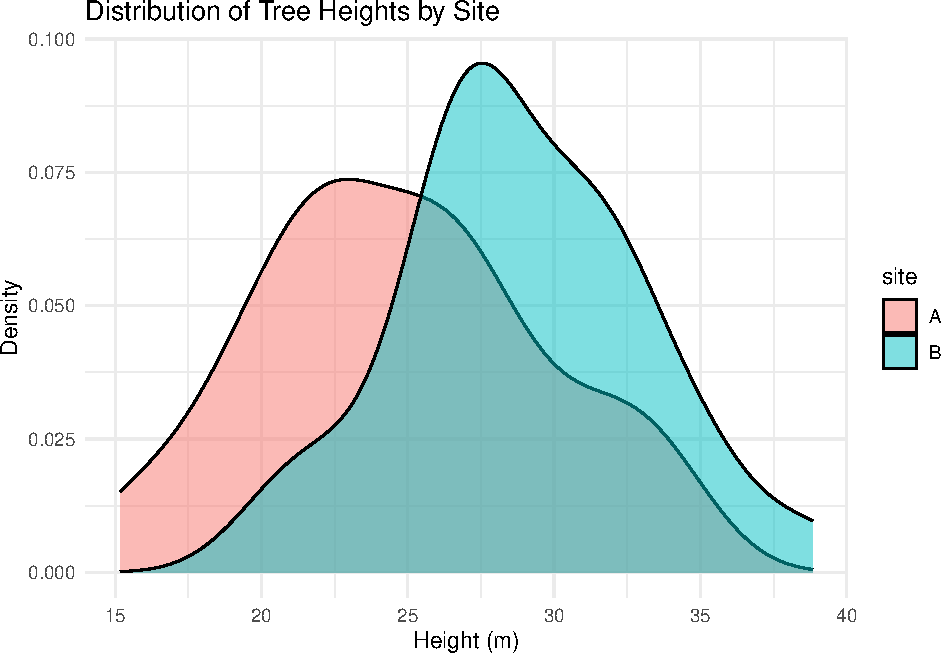
\includegraphics[keepaspectratio]{chapters/04-hypothesis-testing_files/figure-pdf/unnamed-chunk-5-1.pdf}}

\begin{Shaded}
\begin{Highlighting}[]
\CommentTok{\# Add mean lines}
\FunctionTok{ggplot}\NormalTok{(tree\_data, }\FunctionTok{aes}\NormalTok{(}\AttributeTok{x =}\NormalTok{ height, }\AttributeTok{fill =}\NormalTok{ site)) }\SpecialCharTok{+}
  \FunctionTok{geom\_density}\NormalTok{(}\AttributeTok{alpha =} \FloatTok{0.5}\NormalTok{) }\SpecialCharTok{+}
  \FunctionTok{geom\_vline}\NormalTok{(}\AttributeTok{xintercept =} \FunctionTok{mean}\NormalTok{(site\_A), }\AttributeTok{color =} \StringTok{"red"}\NormalTok{, }\AttributeTok{linetype =} \StringTok{"dashed"}\NormalTok{) }\SpecialCharTok{+}
  \FunctionTok{geom\_vline}\NormalTok{(}\AttributeTok{xintercept =} \FunctionTok{mean}\NormalTok{(site\_B), }\AttributeTok{color =} \StringTok{"blue"}\NormalTok{, }\AttributeTok{linetype =} \StringTok{"dashed"}\NormalTok{) }\SpecialCharTok{+}
  \FunctionTok{labs}\NormalTok{(}\AttributeTok{title =} \StringTok{"Distribution of Tree Heights by Site"}\NormalTok{,}
       \AttributeTok{x =} \StringTok{"Height (m)"}\NormalTok{,}
       \AttributeTok{y =} \StringTok{"Density"}\NormalTok{) }\SpecialCharTok{+}
  \FunctionTok{theme\_minimal}\NormalTok{()}
\end{Highlighting}
\end{Shaded}

\pandocbounded{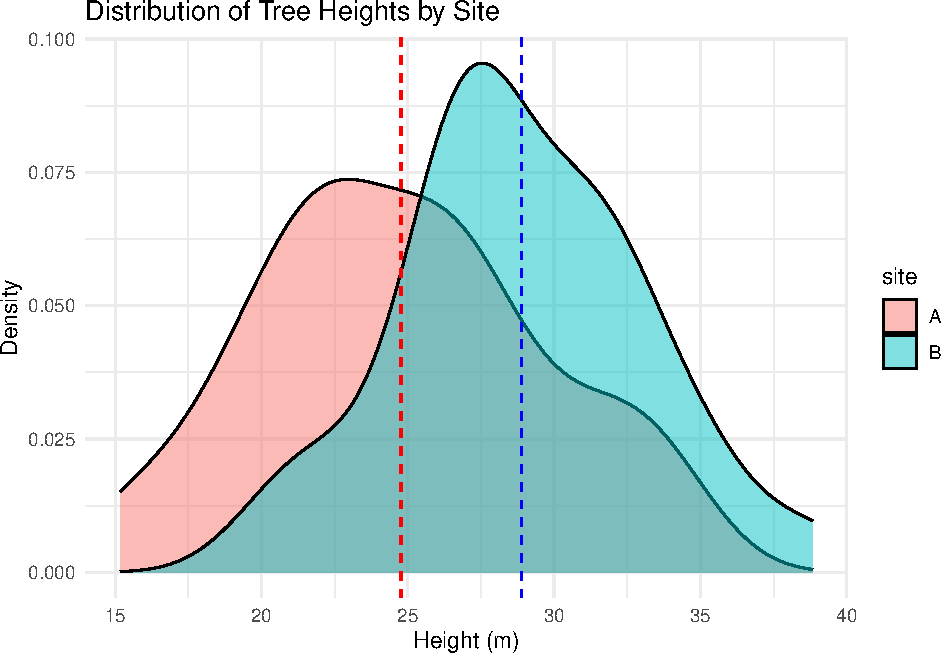
\includegraphics[keepaspectratio]{chapters/04-hypothesis-testing_files/figure-pdf/unnamed-chunk-5-2.pdf}}

\subsection{Paired Samples t-Test}\label{paired-samples-t-test}

The paired samples t-test is used when: - Measurements are taken from
the same subjects under different conditions - The differences between
pairs are approximately normally distributed

\begin{Shaded}
\begin{Highlighting}[]
\CommentTok{\# Simulate paired data (e.g., tree growth before and after treatment)}
\FunctionTok{set.seed}\NormalTok{(}\DecValTok{789}\NormalTok{)}
\NormalTok{before\_treatment }\OtherTok{\textless{}{-}} \FunctionTok{rnorm}\NormalTok{(}\DecValTok{20}\NormalTok{, }\AttributeTok{mean =} \DecValTok{15}\NormalTok{, }\AttributeTok{sd =} \DecValTok{3}\NormalTok{)}
\NormalTok{after\_treatment }\OtherTok{\textless{}{-}}\NormalTok{ before\_treatment }\SpecialCharTok{+} \FunctionTok{rnorm}\NormalTok{(}\DecValTok{20}\NormalTok{, }\AttributeTok{mean =} \FloatTok{2.5}\NormalTok{, }\AttributeTok{sd =} \DecValTok{1}\NormalTok{)  }\CommentTok{\# Growth effect}

\CommentTok{\# Create a data frame}
\NormalTok{growth\_data }\OtherTok{\textless{}{-}} \FunctionTok{data.frame}\NormalTok{(}
  \AttributeTok{tree\_id =} \DecValTok{1}\SpecialCharTok{:}\DecValTok{20}\NormalTok{,}
  \AttributeTok{before =}\NormalTok{ before\_treatment,}
  \AttributeTok{after =}\NormalTok{ after\_treatment,}
  \AttributeTok{difference =}\NormalTok{ after\_treatment }\SpecialCharTok{{-}}\NormalTok{ before\_treatment}
\NormalTok{)}

\CommentTok{\# Visualize paired data}
\NormalTok{growth\_long }\OtherTok{\textless{}{-}}\NormalTok{ reshape2}\SpecialCharTok{::}\FunctionTok{melt}\NormalTok{(growth\_data[, }\FunctionTok{c}\NormalTok{(}\StringTok{"tree\_id"}\NormalTok{, }\StringTok{"before"}\NormalTok{, }\StringTok{"after"}\NormalTok{)], }
                             \AttributeTok{id.vars =} \StringTok{"tree\_id"}\NormalTok{, }
                             \AttributeTok{variable.name =} \StringTok{"time"}\NormalTok{, }
                             \AttributeTok{value.name =} \StringTok{"height"}\NormalTok{)}

\FunctionTok{ggplot}\NormalTok{(growth\_long, }\FunctionTok{aes}\NormalTok{(}\AttributeTok{x =}\NormalTok{ time, }\AttributeTok{y =}\NormalTok{ height, }\AttributeTok{group =}\NormalTok{ tree\_id)) }\SpecialCharTok{+}
  \FunctionTok{geom\_line}\NormalTok{(}\AttributeTok{alpha =} \FloatTok{0.3}\NormalTok{) }\SpecialCharTok{+}
  \FunctionTok{geom\_point}\NormalTok{(}\FunctionTok{aes}\NormalTok{(}\AttributeTok{color =}\NormalTok{ time), }\AttributeTok{size =} \DecValTok{3}\NormalTok{) }\SpecialCharTok{+}
  \FunctionTok{labs}\NormalTok{(}\AttributeTok{title =} \StringTok{"Tree Heights Before and After Treatment"}\NormalTok{,}
       \AttributeTok{x =} \StringTok{"Time"}\NormalTok{,}
       \AttributeTok{y =} \StringTok{"Height (m)"}\NormalTok{) }\SpecialCharTok{+}
  \FunctionTok{theme\_minimal}\NormalTok{()}
\end{Highlighting}
\end{Shaded}

\pandocbounded{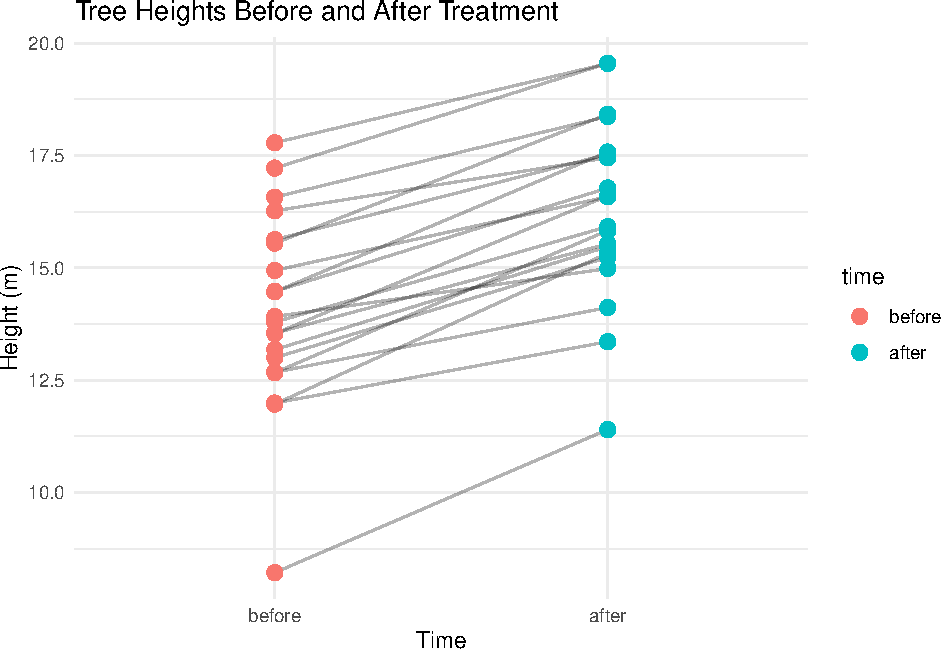
\includegraphics[keepaspectratio]{chapters/04-hypothesis-testing_files/figure-pdf/unnamed-chunk-6-1.pdf}}

\begin{Shaded}
\begin{Highlighting}[]
\CommentTok{\# Perform a paired t{-}test}
\NormalTok{paired\_result }\OtherTok{\textless{}{-}} \FunctionTok{t.test}\NormalTok{(growth\_data}\SpecialCharTok{$}\NormalTok{after, growth\_data}\SpecialCharTok{$}\NormalTok{before, }\AttributeTok{paired =} \ConstantTok{TRUE}\NormalTok{)}
\FunctionTok{print}\NormalTok{(paired\_result)}
\end{Highlighting}
\end{Shaded}

\begin{verbatim}

    Paired t-test

data:  growth_data$after and growth_data$before
t = 13.843, df = 19, p-value = 2.239e-11
alternative hypothesis: true mean difference is not equal to 0
95 percent confidence interval:
 1.874955 2.542925
sample estimates:
mean difference 
        2.20894 
\end{verbatim}

\section{Non-Parametric Tests}\label{non-parametric-tests}

Non-parametric tests are used when the assumptions of parametric tests
(like normality) are violated.

\subsection{Mann-Whitney U Test (Wilcoxon Rank-Sum
Test)}\label{mann-whitney-u-test-wilcoxon-rank-sum-test}

This is a non-parametric alternative to the independent samples t-test.

\begin{Shaded}
\begin{Highlighting}[]
\CommentTok{\# Simulate non{-}normal data (e.g., species counts in two habitats)}
\FunctionTok{set.seed}\NormalTok{(}\DecValTok{101}\NormalTok{)}
\NormalTok{habitat\_A }\OtherTok{\textless{}{-}} \FunctionTok{rpois}\NormalTok{(}\DecValTok{25}\NormalTok{, }\AttributeTok{lambda =} \DecValTok{8}\NormalTok{)  }\CommentTok{\# Poisson distribution for count data}
\NormalTok{habitat\_B }\OtherTok{\textless{}{-}} \FunctionTok{rpois}\NormalTok{(}\DecValTok{25}\NormalTok{, }\AttributeTok{lambda =} \DecValTok{12}\NormalTok{)}

\CommentTok{\# Create a data frame}
\NormalTok{species\_data }\OtherTok{\textless{}{-}} \FunctionTok{data.frame}\NormalTok{(}
  \AttributeTok{count =} \FunctionTok{c}\NormalTok{(habitat\_A, habitat\_B),}
  \AttributeTok{habitat =} \FunctionTok{factor}\NormalTok{(}\FunctionTok{rep}\NormalTok{(}\FunctionTok{c}\NormalTok{(}\StringTok{"A"}\NormalTok{, }\StringTok{"B"}\NormalTok{), }\AttributeTok{each =} \DecValTok{25}\NormalTok{))}
\NormalTok{)}

\CommentTok{\# Visualize the data}
\FunctionTok{ggplot}\NormalTok{(species\_data, }\FunctionTok{aes}\NormalTok{(}\AttributeTok{x =}\NormalTok{ habitat, }\AttributeTok{y =}\NormalTok{ count, }\AttributeTok{fill =}\NormalTok{ habitat)) }\SpecialCharTok{+}
  \FunctionTok{geom\_boxplot}\NormalTok{() }\SpecialCharTok{+}
  \FunctionTok{labs}\NormalTok{(}\AttributeTok{title =} \StringTok{"Species Counts by Habitat"}\NormalTok{,}
       \AttributeTok{x =} \StringTok{"Habitat"}\NormalTok{,}
       \AttributeTok{y =} \StringTok{"Count"}\NormalTok{) }\SpecialCharTok{+}
  \FunctionTok{theme\_minimal}\NormalTok{()}
\end{Highlighting}
\end{Shaded}

\pandocbounded{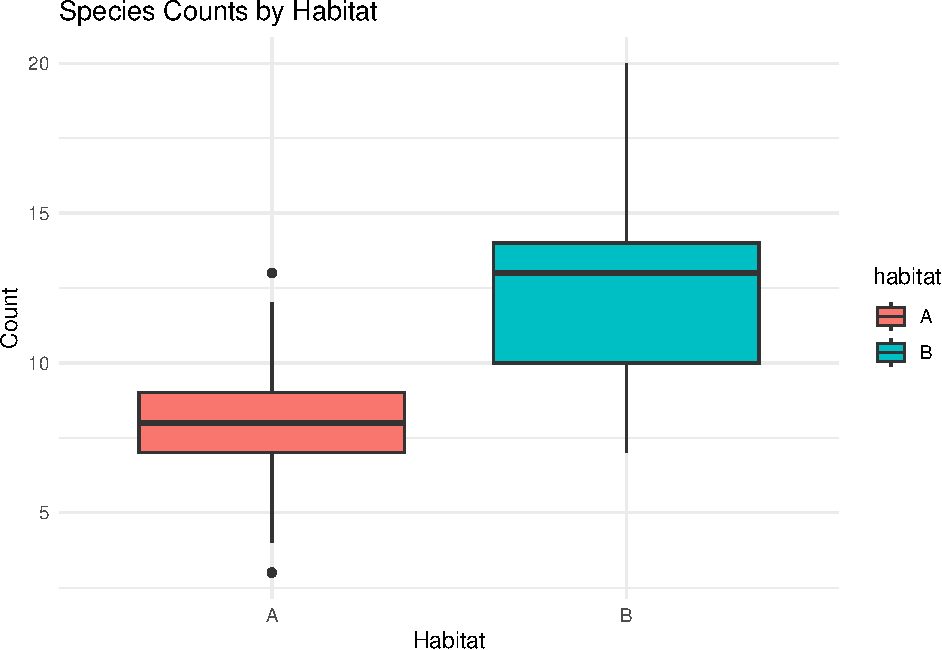
\includegraphics[keepaspectratio]{chapters/04-hypothesis-testing_files/figure-pdf/unnamed-chunk-7-1.pdf}}

\begin{Shaded}
\begin{Highlighting}[]
\CommentTok{\# Check for normality}
\FunctionTok{shapiro.test}\NormalTok{(habitat\_A)}
\end{Highlighting}
\end{Shaded}

\begin{verbatim}

    Shapiro-Wilk normality test

data:  habitat_A
W = 0.97173, p-value = 0.6892
\end{verbatim}

\begin{Shaded}
\begin{Highlighting}[]
\FunctionTok{shapiro.test}\NormalTok{(habitat\_B)}
\end{Highlighting}
\end{Shaded}

\begin{verbatim}

    Shapiro-Wilk normality test

data:  habitat_B
W = 0.97562, p-value = 0.7869
\end{verbatim}

\begin{Shaded}
\begin{Highlighting}[]
\CommentTok{\# Perform Mann{-}Whitney U test}
\NormalTok{wilcox\_result }\OtherTok{\textless{}{-}} \FunctionTok{wilcox.test}\NormalTok{(count }\SpecialCharTok{\textasciitilde{}}\NormalTok{ habitat, }\AttributeTok{data =}\NormalTok{ species\_data)}
\FunctionTok{print}\NormalTok{(wilcox\_result)}
\end{Highlighting}
\end{Shaded}

\begin{verbatim}

    Wilcoxon rank sum test with continuity correction

data:  count by habitat
W = 88.5, p-value = 1.308e-05
alternative hypothesis: true location shift is not equal to 0
\end{verbatim}

\subsection{Wilcoxon Signed-Rank Test}\label{wilcoxon-signed-rank-test}

This is a non-parametric alternative to the paired samples t-test.

\begin{Shaded}
\begin{Highlighting}[]
\CommentTok{\# Simulate non{-}normal paired data}
\FunctionTok{set.seed}\NormalTok{(}\DecValTok{202}\NormalTok{)}
\NormalTok{before\_restoration }\OtherTok{\textless{}{-}} \FunctionTok{rpois}\NormalTok{(}\DecValTok{20}\NormalTok{, }\AttributeTok{lambda =} \DecValTok{5}\NormalTok{)}
\NormalTok{after\_restoration }\OtherTok{\textless{}{-}}\NormalTok{ before\_restoration }\SpecialCharTok{+} \FunctionTok{rpois}\NormalTok{(}\DecValTok{20}\NormalTok{, }\AttributeTok{lambda =} \DecValTok{3}\NormalTok{)}

\CommentTok{\# Create a data frame}
\NormalTok{restoration\_data }\OtherTok{\textless{}{-}} \FunctionTok{data.frame}\NormalTok{(}
  \AttributeTok{site\_id =} \DecValTok{1}\SpecialCharTok{:}\DecValTok{20}\NormalTok{,}
  \AttributeTok{before =}\NormalTok{ before\_restoration,}
  \AttributeTok{after =}\NormalTok{ after\_restoration,}
  \AttributeTok{difference =}\NormalTok{ after\_restoration }\SpecialCharTok{{-}}\NormalTok{ before\_restoration}
\NormalTok{)}

\CommentTok{\# Visualize paired data}
\NormalTok{restoration\_long }\OtherTok{\textless{}{-}}\NormalTok{ reshape2}\SpecialCharTok{::}\FunctionTok{melt}\NormalTok{(restoration\_data[, }\FunctionTok{c}\NormalTok{(}\StringTok{"site\_id"}\NormalTok{, }\StringTok{"before"}\NormalTok{, }\StringTok{"after"}\NormalTok{)], }
                                  \AttributeTok{id.vars =} \StringTok{"site\_id"}\NormalTok{, }
                                  \AttributeTok{variable.name =} \StringTok{"time"}\NormalTok{, }
                                  \AttributeTok{value.name =} \StringTok{"species\_count"}\NormalTok{)}

\FunctionTok{ggplot}\NormalTok{(restoration\_long, }\FunctionTok{aes}\NormalTok{(}\AttributeTok{x =}\NormalTok{ time, }\AttributeTok{y =}\NormalTok{ species\_count, }\AttributeTok{group =}\NormalTok{ site\_id)) }\SpecialCharTok{+}
  \FunctionTok{geom\_line}\NormalTok{(}\AttributeTok{alpha =} \FloatTok{0.3}\NormalTok{) }\SpecialCharTok{+}
  \FunctionTok{geom\_point}\NormalTok{(}\FunctionTok{aes}\NormalTok{(}\AttributeTok{color =}\NormalTok{ time), }\AttributeTok{size =} \DecValTok{3}\NormalTok{) }\SpecialCharTok{+}
  \FunctionTok{labs}\NormalTok{(}\AttributeTok{title =} \StringTok{"Species Counts Before and After Restoration"}\NormalTok{,}
       \AttributeTok{x =} \StringTok{"Time"}\NormalTok{,}
       \AttributeTok{y =} \StringTok{"Species Count"}\NormalTok{) }\SpecialCharTok{+}
  \FunctionTok{theme\_minimal}\NormalTok{()}
\end{Highlighting}
\end{Shaded}

\pandocbounded{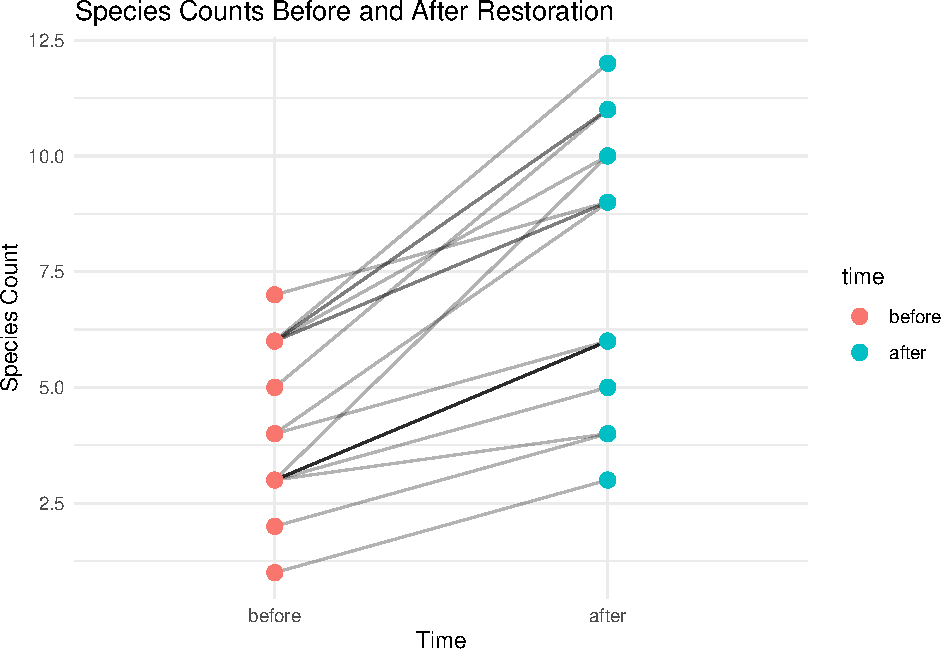
\includegraphics[keepaspectratio]{chapters/04-hypothesis-testing_files/figure-pdf/unnamed-chunk-8-1.pdf}}

\begin{Shaded}
\begin{Highlighting}[]
\CommentTok{\# Perform Wilcoxon signed{-}rank test}
\NormalTok{wilcox\_paired\_result }\OtherTok{\textless{}{-}} \FunctionTok{wilcox.test}\NormalTok{(restoration\_data}\SpecialCharTok{$}\NormalTok{after, restoration\_data}\SpecialCharTok{$}\NormalTok{before, }\AttributeTok{paired =} \ConstantTok{TRUE}\NormalTok{)}
\FunctionTok{print}\NormalTok{(wilcox\_paired\_result)}
\end{Highlighting}
\end{Shaded}

\begin{verbatim}

    Wilcoxon signed rank test with continuity correction

data:  restoration_data$after and restoration_data$before
V = 210, p-value = 8.527e-05
alternative hypothesis: true location shift is not equal to 0
\end{verbatim}

\section{Confidence Intervals}\label{confidence-intervals}

Confidence intervals provide a range of plausible values for a
population parameter.

\begin{Shaded}
\begin{Highlighting}[]
\CommentTok{\# Calculate 95\% confidence interval for mean tree height in Site A}
\NormalTok{ci\_result }\OtherTok{\textless{}{-}} \FunctionTok{t.test}\NormalTok{(site\_A)}
\FunctionTok{print}\NormalTok{(ci\_result}\SpecialCharTok{$}\NormalTok{conf.int)}
\end{Highlighting}
\end{Shaded}

\begin{verbatim}
[1] 22.93287 26.59610
attr(,"conf.level")
[1] 0.95
\end{verbatim}

\begin{Shaded}
\begin{Highlighting}[]
\CommentTok{\# Visualize confidence interval}
\NormalTok{mean\_height }\OtherTok{\textless{}{-}} \FunctionTok{mean}\NormalTok{(site\_A)}
\NormalTok{ci\_lower }\OtherTok{\textless{}{-}}\NormalTok{ ci\_result}\SpecialCharTok{$}\NormalTok{conf.int[}\DecValTok{1}\NormalTok{]}
\NormalTok{ci\_upper }\OtherTok{\textless{}{-}}\NormalTok{ ci\_result}\SpecialCharTok{$}\NormalTok{conf.int[}\DecValTok{2}\NormalTok{]}

\FunctionTok{ggplot}\NormalTok{(}\FunctionTok{data.frame}\NormalTok{(}\AttributeTok{height =}\NormalTok{ site\_A), }\FunctionTok{aes}\NormalTok{(}\AttributeTok{x =}\NormalTok{ height)) }\SpecialCharTok{+}
  \FunctionTok{geom\_histogram}\NormalTok{(}\AttributeTok{bins =} \DecValTok{10}\NormalTok{, }\AttributeTok{fill =} \StringTok{"skyblue"}\NormalTok{, }\AttributeTok{color =} \StringTok{"white"}\NormalTok{) }\SpecialCharTok{+}
  \FunctionTok{geom\_vline}\NormalTok{(}\AttributeTok{xintercept =}\NormalTok{ mean\_height, }\AttributeTok{color =} \StringTok{"red"}\NormalTok{, }\AttributeTok{size =} \DecValTok{1}\NormalTok{) }\SpecialCharTok{+}
  \FunctionTok{geom\_vline}\NormalTok{(}\AttributeTok{xintercept =}\NormalTok{ ci\_lower, }\AttributeTok{color =} \StringTok{"blue"}\NormalTok{, }\AttributeTok{linetype =} \StringTok{"dashed"}\NormalTok{) }\SpecialCharTok{+}
  \FunctionTok{geom\_vline}\NormalTok{(}\AttributeTok{xintercept =}\NormalTok{ ci\_upper, }\AttributeTok{color =} \StringTok{"blue"}\NormalTok{, }\AttributeTok{linetype =} \StringTok{"dashed"}\NormalTok{) }\SpecialCharTok{+}
  \FunctionTok{annotate}\NormalTok{(}\StringTok{"rect"}\NormalTok{, }\AttributeTok{xmin =}\NormalTok{ ci\_lower, }\AttributeTok{xmax =}\NormalTok{ ci\_upper, }\AttributeTok{ymin =} \DecValTok{0}\NormalTok{, }\AttributeTok{ymax =} \ConstantTok{Inf}\NormalTok{, }
           \AttributeTok{fill =} \StringTok{"blue"}\NormalTok{, }\AttributeTok{alpha =} \FloatTok{0.1}\NormalTok{) }\SpecialCharTok{+}
  \FunctionTok{labs}\NormalTok{(}\AttributeTok{title =} \StringTok{"Tree Heights in Site A with 95\% Confidence Interval"}\NormalTok{,}
       \AttributeTok{x =} \StringTok{"Height (m)"}\NormalTok{,}
       \AttributeTok{y =} \StringTok{"Frequency"}\NormalTok{) }\SpecialCharTok{+}
  \FunctionTok{annotate}\NormalTok{(}\StringTok{"text"}\NormalTok{, }\AttributeTok{x =}\NormalTok{ mean\_height, }\AttributeTok{y =} \DecValTok{8}\NormalTok{, }\AttributeTok{label =} \StringTok{"Mean"}\NormalTok{, }\AttributeTok{color =} \StringTok{"red"}\NormalTok{) }\SpecialCharTok{+}
  \FunctionTok{annotate}\NormalTok{(}\StringTok{"text"}\NormalTok{, }\AttributeTok{x =}\NormalTok{ ci\_lower }\SpecialCharTok{{-}} \DecValTok{1}\NormalTok{, }\AttributeTok{y =} \DecValTok{6}\NormalTok{, }\AttributeTok{label =} \StringTok{"Lower CI"}\NormalTok{, }\AttributeTok{color =} \StringTok{"blue"}\NormalTok{) }\SpecialCharTok{+}
  \FunctionTok{annotate}\NormalTok{(}\StringTok{"text"}\NormalTok{, }\AttributeTok{x =}\NormalTok{ ci\_upper }\SpecialCharTok{+} \DecValTok{1}\NormalTok{, }\AttributeTok{y =} \DecValTok{6}\NormalTok{, }\AttributeTok{label =} \StringTok{"Upper CI"}\NormalTok{, }\AttributeTok{color =} \StringTok{"blue"}\NormalTok{) }\SpecialCharTok{+}
  \FunctionTok{theme\_minimal}\NormalTok{()}
\end{Highlighting}
\end{Shaded}

\pandocbounded{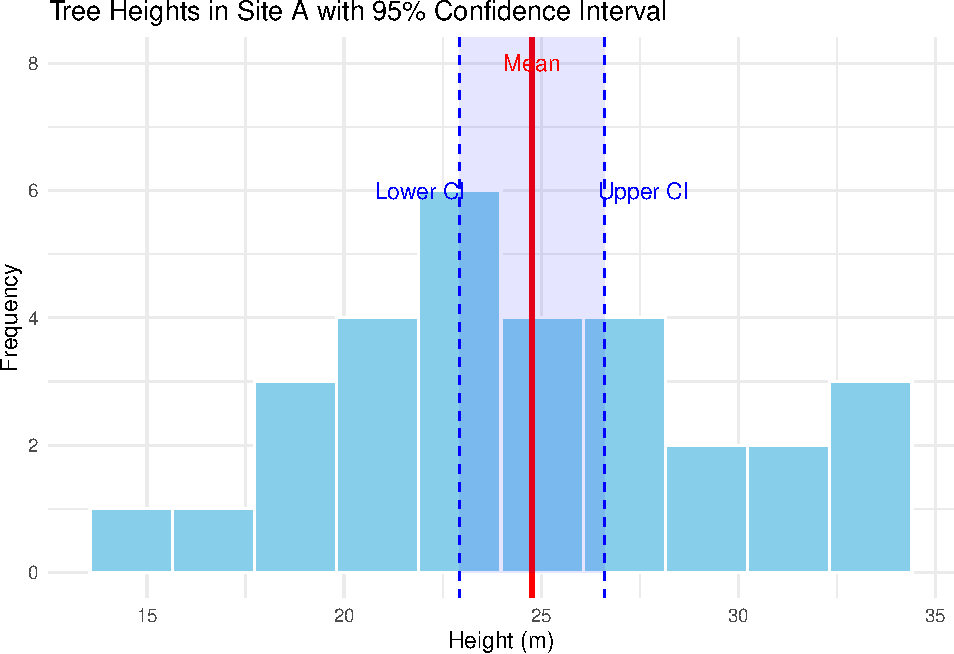
\includegraphics[keepaspectratio]{chapters/04-hypothesis-testing_files/figure-pdf/unnamed-chunk-9-1.pdf}}

\section{Exercises}\label{exercises-3}

\begin{enumerate}
\def\labelenumi{\arabic{enumi}.}
\tightlist
\item
  Formulate a hypothesis about a relationship between two variables in
  the forest inventory dataset.
\item
  Conduct an appropriate statistical test to evaluate your hypothesis.
\item
  Calculate the effect size for your test.
\item
  Interpret the results, including the p-value and effect size.
\item
  Create a visualization that effectively communicates your findings.
\end{enumerate}

\section{Summary}\label{summary-3}

In this chapter, we've covered the fundamental concepts and techniques
of hypothesis testing in ecological and forestry research:

\begin{itemize}
\tightlist
\item
  Formulating null and alternative hypotheses
\item
  Understanding p-values and significance levels
\item
  Recognizing Type I and Type II errors
\item
  Calculating and interpreting statistical power
\item
  Conducting one-sample, two-sample, and paired tests
\item
  Using non-parametric alternatives when necessary
\item
  Calculating and interpreting confidence intervals
\end{itemize}

These statistical tools allow researchers to make informed inferences
about populations based on sample data, helping to advance knowledge in
ecology and forestry.

\section{Statistical Power}\label{statistical-power-1}

Statistical power is the probability of correctly rejecting the null
hypothesis when it is false. It is influenced by:

\begin{enumerate}
\def\labelenumi{\arabic{enumi}.}
\tightlist
\item
  Sample size
\item
  Effect size
\item
  Significance level (α)
\item
  Variability in the data
\end{enumerate}

\chapter{Demonstrate power calculation for a
t-test}\label{demonstrate-power-calculation-for-a-t-test}

library(pwr)

\chapter{Calculate power for our
example}\label{calculate-power-for-our-example}

effect\_size \textless- (28 - 25) / 5 \# (mean difference) / standard
deviation power\_result \textless- pwr.t.test( n = 30, \# Sample size
per group d = effect\_size, \# Cohen's d effect size sig.level = 0.05,
\# Significance level type = ``two.sample'', \# Two-sample t-test
alternative = ``two.sided'' \# Two-sided alternative )

print(power\_result)

\chapter{Calculate required sample size for 80\%
power}\label{calculate-required-sample-size-for-80-power}

sample\_size\_result \textless- pwr.t.test( d = effect\_size, \# Cohen's
d effect size sig.level = 0.05, \# Significance level power = 0.8, \#
Desired power type = ``two.sample'', \# Two-sample t-test alternative =
``two.sided'' \# Two-sided alternative )

print(sample\_size\_result)

\chapter{Common Statistical Tests}\label{common-statistical-tests}

\section{Introduction}\label{introduction-3}

This chapter explores common statistical tests used in natural sciences
research. Building on the hypothesis testing framework introduced in the
previous chapter, we'll examine specific tests for different research
scenarios and data types.

\section{Choosing the Right Statistical
Test}\label{choosing-the-right-statistical-test}

Selecting the appropriate statistical test depends on several factors:

\begin{enumerate}
\def\labelenumi{\arabic{enumi}.}
\tightlist
\item
  \textbf{Research Question}: What you're trying to determine
\item
  \textbf{Data Type}: Categorical, continuous, or ordinal
\item
  \textbf{Number of Groups}: One, two, or multiple groups
\item
  \textbf{Data Distribution}: Normal or non-normal
\item
  \textbf{Independence}: Whether observations are independent or related
\end{enumerate}

\subsection{Decision Tree for Common
Tests}\label{decision-tree-for-common-tests}

\textbf{Decision Tree for Selecting Statistical Tests:}

\begin{enumerate}
\def\labelenumi{\arabic{enumi}.}
\tightlist
\item
  \textbf{For One Variable:}

  \begin{itemize}
  \tightlist
  \item
    \textbf{One Sample:}

    \begin{itemize}
    \tightlist
    \item
      Normal, Continuous → One-Sample t-Test
    \item
      Non-normal, Continuous → Wilcoxon Signed-Rank Test
    \item
      Categorical → Binomial Test
    \end{itemize}
  \item
    \textbf{Two Samples:}

    \begin{itemize}
    \tightlist
    \item
      Normal, Continuous, Independent → Independent t-Test
    \item
      Normal, Continuous, Related → Paired t-Test
    \item
      Non-normal, Continuous, Independent → Mann-Whitney U Test
    \item
      Non-normal, Continuous, Related → Wilcoxon Signed-Rank Test
    \item
      Categorical, Independent → Chi-Square Test
    \item
      Categorical, Related → McNemar Test
    \end{itemize}
  \item
    \textbf{Multiple Samples:}

    \begin{itemize}
    \tightlist
    \item
      Normal, Continuous, Independent → ANOVA
    \item
      Normal, Continuous, Related → Repeated Measures ANOVA
    \item
      Non-normal, Continuous, Independent → Kruskal-Wallis Test
    \item
      Non-normal, Continuous, Related → Friedman Test
    \item
      Categorical → Chi-Square Test
    \end{itemize}
  \end{itemize}
\item
  \textbf{For Two Variables:}

  \begin{itemize}
  \tightlist
  \item
    Normal, Continuous → Pearson Correlation
  \item
    Non-normal or Ordinal → Spearman Correlation
  \item
    Continuous Predictor \& Outcome → Linear Regression
  \item
    Continuous Predictor, Binary Outcome → Logistic Regression
  \end{itemize}
\item
  \textbf{For Multiple Variables:}

  \begin{itemize}
  \tightlist
  \item
    Multiple Continuous Outcomes → MANOVA
  \item
    Dimension Reduction → Principal Component Analysis
  \item
    Grouping → Cluster Analysis
  \end{itemize}
\end{enumerate}

\section{Parametric vs.~Non-Parametric
Tests}\label{parametric-vs.-non-parametric-tests}

\subsection{Parametric Tests}\label{parametric-tests}

Parametric tests make assumptions about the underlying population
distribution, typically that the data follows a normal distribution.
Common parametric tests include:

\begin{itemize}
\tightlist
\item
  t-tests
\item
  ANOVA
\item
  Pearson correlation
\item
  Linear regression
\end{itemize}

\subsection{Non-Parametric Tests}\label{non-parametric-tests-1}

Non-parametric tests make fewer assumptions about the population
distribution and are useful when data doesn't meet the assumptions of
parametric tests. Common non-parametric tests include:

\begin{itemize}
\tightlist
\item
  Mann-Whitney U test
\item
  Wilcoxon signed-rank test
\item
  Kruskal-Wallis test
\item
  Spearman correlation
\end{itemize}

\subsection{Checking Assumptions}\label{checking-assumptions}

Before applying a parametric test, it's essential to check if your data
meets the necessary assumptions. Let's use our crop yield dataset to
demonstrate:

\begin{Shaded}
\begin{Highlighting}[]
\CommentTok{\# Load necessary libraries}
\FunctionTok{library}\NormalTok{(tidyverse)}

\CommentTok{\# Load the crop yield dataset}
\NormalTok{crop\_yields }\OtherTok{\textless{}{-}} \FunctionTok{read\_csv}\NormalTok{(}\StringTok{"../data/agriculture/crop\_yields.csv"}\NormalTok{)}

\CommentTok{\# View column names to see how R has formatted them}
\FunctionTok{names}\NormalTok{(crop\_yields)}
\end{Highlighting}
\end{Shaded}

\begin{verbatim}
 [1] "Entity"                           "Code"                            
 [3] "Year"                             "Wheat (tonnes per hectare)"      
 [5] "Rice (tonnes per hectare)"        "Maize (tonnes per hectare)"      
 [7] "Soybeans (tonnes per hectare)"    "Potatoes (tonnes per hectare)"   
 [9] "Beans (tonnes per hectare)"       "Peas (tonnes per hectare)"       
[11] "Cassava (tonnes per hectare)"     "Barley (tonnes per hectare)"     
[13] "Cocoa beans (tonnes per hectare)" "Bananas (tonnes per hectare)"    
\end{verbatim}

\begin{Shaded}
\begin{Highlighting}[]
\CommentTok{\# Extract wheat yields for analysis}
\NormalTok{wheat\_yields }\OtherTok{\textless{}{-}}\NormalTok{ crop\_yields }\SpecialCharTok{\%\textgreater{}\%}
  \FunctionTok{filter}\NormalTok{(}\SpecialCharTok{!}\FunctionTok{is.na}\NormalTok{(}\StringTok{\textasciigrave{}}\AttributeTok{Wheat (tonnes per hectare)}\StringTok{\textasciigrave{}}\NormalTok{)) }\SpecialCharTok{\%\textgreater{}\%}
  \FunctionTok{select}\NormalTok{(Entity, Year, }\StringTok{\textasciigrave{}}\AttributeTok{Wheat (tonnes per hectare)}\StringTok{\textasciigrave{}}\NormalTok{)}

\CommentTok{\# View the first few rows}
\FunctionTok{head}\NormalTok{(wheat\_yields)}
\end{Highlighting}
\end{Shaded}

\begin{verbatim}
# A tibble: 6 x 3
  Entity       Year `Wheat (tonnes per hectare)`
  <chr>       <dbl>                        <dbl>
1 Afghanistan  1961                        1.02 
2 Afghanistan  1962                        0.974
3 Afghanistan  1963                        0.832
4 Afghanistan  1964                        0.951
5 Afghanistan  1965                        0.972
6 Afghanistan  1966                        0.867
\end{verbatim}

\begin{Shaded}
\begin{Highlighting}[]
\CommentTok{\# Check for normality}
\CommentTok{\# Visual methods}
\FunctionTok{par}\NormalTok{(}\AttributeTok{mfrow =} \FunctionTok{c}\NormalTok{(}\DecValTok{1}\NormalTok{, }\DecValTok{2}\NormalTok{))}
\FunctionTok{hist}\NormalTok{(wheat\_yields}\SpecialCharTok{$}\StringTok{\textasciigrave{}}\AttributeTok{Wheat (tonnes per hectare)}\StringTok{\textasciigrave{}}\NormalTok{, }\AttributeTok{main =} \StringTok{"Histogram of Wheat Yields"}\NormalTok{, }\AttributeTok{xlab =} \StringTok{"Yield (tonnes/hectare)"}\NormalTok{)}
\FunctionTok{qqnorm}\NormalTok{(wheat\_yields}\SpecialCharTok{$}\StringTok{\textasciigrave{}}\AttributeTok{Wheat (tonnes per hectare)}\StringTok{\textasciigrave{}}\NormalTok{); }\FunctionTok{qqline}\NormalTok{(wheat\_yields}\SpecialCharTok{$}\StringTok{\textasciigrave{}}\AttributeTok{Wheat (tonnes per hectare)}\StringTok{\textasciigrave{}}\NormalTok{, }\AttributeTok{col =} \StringTok{"red"}\NormalTok{)}
\end{Highlighting}
\end{Shaded}

\pandocbounded{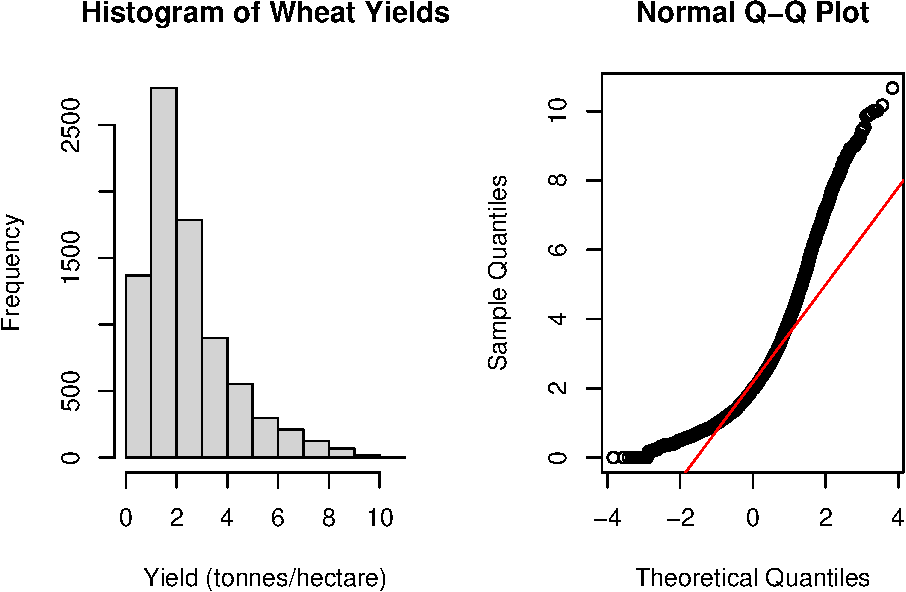
\includegraphics[keepaspectratio]{chapters/05-statistical-tests_files/figure-pdf/unnamed-chunk-2-1.pdf}}

\begin{Shaded}
\begin{Highlighting}[]
\CommentTok{\# Statistical test for normality}
\FunctionTok{shapiro.test}\NormalTok{(}\FunctionTok{sample}\NormalTok{(wheat\_yields}\SpecialCharTok{$}\StringTok{\textasciigrave{}}\AttributeTok{Wheat (tonnes per hectare)}\StringTok{\textasciigrave{}}\NormalTok{, }\FunctionTok{min}\NormalTok{(}\DecValTok{5000}\NormalTok{, }\FunctionTok{length}\NormalTok{(wheat\_yields}\SpecialCharTok{$}\StringTok{\textasciigrave{}}\AttributeTok{Wheat (tonnes per hectare)}\StringTok{\textasciigrave{}}\NormalTok{))))}
\end{Highlighting}
\end{Shaded}

\begin{verbatim}

    Shapiro-Wilk normality test

data:  sample(wheat_yields$`Wheat (tonnes per hectare)`, min(5000, length(wheat_yields$`Wheat (tonnes per hectare)`)))
W = 0.8737, p-value < 2.2e-16
\end{verbatim}

\section{Tests for Comparing Groups}\label{tests-for-comparing-groups}

\subsection{t-Tests}\label{t-tests}

\subsubsection{Independent Samples
t-Test}\label{independent-samples-t-test-1}

Used to compare means between two independent groups. Let's compare
wheat yields between two time periods:

\begin{Shaded}
\begin{Highlighting}[]
\CommentTok{\# Create two groups: early period (before 2000) and recent period (2000 onwards)}
\NormalTok{crop\_yields\_grouped }\OtherTok{\textless{}{-}}\NormalTok{ crop\_yields }\SpecialCharTok{\%\textgreater{}\%}
  \FunctionTok{filter}\NormalTok{(}\SpecialCharTok{!}\FunctionTok{is.na}\NormalTok{(}\StringTok{\textasciigrave{}}\AttributeTok{Wheat (tonnes per hectare)}\StringTok{\textasciigrave{}}\NormalTok{) }\SpecialCharTok{\&}\NormalTok{ Year }\SpecialCharTok{\textgreater{}=} \DecValTok{1960}\NormalTok{) }\SpecialCharTok{\%\textgreater{}\%}
  \FunctionTok{mutate}\NormalTok{(}\AttributeTok{period =} \FunctionTok{ifelse}\NormalTok{(Year }\SpecialCharTok{\textless{}} \DecValTok{2000}\NormalTok{, }\StringTok{"Early Period (pre{-}2000)"}\NormalTok{, }\StringTok{"Recent Period (2000+)"}\NormalTok{))}

\CommentTok{\# Visualize the data}
\FunctionTok{ggplot}\NormalTok{(crop\_yields\_grouped, }\FunctionTok{aes}\NormalTok{(}\AttributeTok{x =}\NormalTok{ period, }\AttributeTok{y =} \StringTok{\textasciigrave{}}\AttributeTok{Wheat (tonnes per hectare)}\StringTok{\textasciigrave{}}\NormalTok{, }\AttributeTok{fill =}\NormalTok{ period)) }\SpecialCharTok{+}
  \FunctionTok{geom\_boxplot}\NormalTok{() }\SpecialCharTok{+}
  \FunctionTok{labs}\NormalTok{(}\AttributeTok{title =} \StringTok{"Wheat Yields by Time Period"}\NormalTok{,}
       \AttributeTok{x =} \StringTok{"Period"}\NormalTok{,}
       \AttributeTok{y =} \StringTok{"Wheat Yield (tonnes/hectare)"}\NormalTok{) }\SpecialCharTok{+}
  \FunctionTok{theme\_minimal}\NormalTok{() }\SpecialCharTok{+}
  \FunctionTok{theme}\NormalTok{(}\AttributeTok{legend.position =} \StringTok{"none"}\NormalTok{)}
\end{Highlighting}
\end{Shaded}

\pandocbounded{\includegraphics[keepaspectratio]{chapters/05-statistical-tests_files/figure-pdf/unnamed-chunk-3-1.pdf}}

\begin{Shaded}
\begin{Highlighting}[]
\CommentTok{\# Perform independent samples t{-}test using formula interface with backticks}
\NormalTok{t\_test\_result }\OtherTok{\textless{}{-}} \FunctionTok{t.test}\NormalTok{(}\StringTok{\textasciigrave{}}\AttributeTok{Wheat (tonnes per hectare)}\StringTok{\textasciigrave{}} \SpecialCharTok{\textasciitilde{}}\NormalTok{ period, }\AttributeTok{data =}\NormalTok{ crop\_yields\_grouped)}
\NormalTok{t\_test\_result}
\end{Highlighting}
\end{Shaded}

\begin{verbatim}

    Welch Two Sample t-test

data:  Wheat (tonnes per hectare) by period
t = -22.335, df = 4970.2, p-value < 2.2e-16
alternative hypothesis: true difference in means between group Early Period (pre-2000) and group Recent Period (2000+) is not equal to 0
95 percent confidence interval:
 -0.9798533 -0.8217198
sample estimates:
mean in group Early Period (pre-2000)   mean in group Recent Period (2000+) 
                             2.109781                              3.010567 
\end{verbatim}

\subsubsection{Paired Samples t-Test}\label{paired-samples-t-test-1}

Used to compare means between two related groups. Let's compare wheat
and rice yields for the same countries and years:

\begin{Shaded}
\begin{Highlighting}[]
\CommentTok{\# Prepare data for paired t{-}test}
\NormalTok{paired\_data }\OtherTok{\textless{}{-}}\NormalTok{ crop\_yields }\SpecialCharTok{\%\textgreater{}\%}
  \FunctionTok{filter}\NormalTok{(}\SpecialCharTok{!}\FunctionTok{is.na}\NormalTok{(}\StringTok{\textasciigrave{}}\AttributeTok{Wheat (tonnes per hectare)}\StringTok{\textasciigrave{}}\NormalTok{) }\SpecialCharTok{\&} \SpecialCharTok{!}\FunctionTok{is.na}\NormalTok{(}\StringTok{\textasciigrave{}}\AttributeTok{Rice (tonnes per hectare)}\StringTok{\textasciigrave{}}\NormalTok{)) }\SpecialCharTok{\%\textgreater{}\%}
  \FunctionTok{select}\NormalTok{(Entity, Year, }\StringTok{\textasciigrave{}}\AttributeTok{Wheat (tonnes per hectare)}\StringTok{\textasciigrave{}}\NormalTok{, }\StringTok{\textasciigrave{}}\AttributeTok{Rice (tonnes per hectare)}\StringTok{\textasciigrave{}}\NormalTok{)}

\CommentTok{\# View the first few rows}
\FunctionTok{head}\NormalTok{(paired\_data)}
\end{Highlighting}
\end{Shaded}

\begin{verbatim}
# A tibble: 6 x 4
  Entity       Year `Wheat (tonnes per hectare)` `Rice (tonnes per hectare)`
  <chr>       <dbl>                        <dbl>                       <dbl>
1 Afghanistan  1961                        1.02                         1.52
2 Afghanistan  1962                        0.974                        1.52
3 Afghanistan  1963                        0.832                        1.52
4 Afghanistan  1964                        0.951                        1.73
5 Afghanistan  1965                        0.972                        1.73
6 Afghanistan  1966                        0.867                        1.52
\end{verbatim}

\begin{Shaded}
\begin{Highlighting}[]
\CommentTok{\# Visualize the paired data}
\NormalTok{paired\_data\_long }\OtherTok{\textless{}{-}}\NormalTok{ paired\_data }\SpecialCharTok{\%\textgreater{}\%}
  \FunctionTok{pivot\_longer}\NormalTok{(}\AttributeTok{cols =} \FunctionTok{c}\NormalTok{(}\StringTok{\textasciigrave{}}\AttributeTok{Wheat (tonnes per hectare)}\StringTok{\textasciigrave{}}\NormalTok{, }\StringTok{\textasciigrave{}}\AttributeTok{Rice (tonnes per hectare)}\StringTok{\textasciigrave{}}\NormalTok{), }\AttributeTok{names\_to =} \StringTok{"Crop"}\NormalTok{, }\AttributeTok{values\_to =} \StringTok{"Yield"}\NormalTok{)}

\FunctionTok{ggplot}\NormalTok{(paired\_data\_long, }\FunctionTok{aes}\NormalTok{(}\AttributeTok{x =}\NormalTok{ Crop, }\AttributeTok{y =}\NormalTok{ Yield, }\AttributeTok{fill =}\NormalTok{ Crop)) }\SpecialCharTok{+}
  \FunctionTok{geom\_boxplot}\NormalTok{() }\SpecialCharTok{+}
  \FunctionTok{labs}\NormalTok{(}\AttributeTok{title =} \StringTok{"Comparison of Wheat and Rice Yields"}\NormalTok{,}
       \AttributeTok{x =} \StringTok{"Crop Type"}\NormalTok{,}
       \AttributeTok{y =} \StringTok{"Yield (tonnes/hectare)"}\NormalTok{) }\SpecialCharTok{+}
  \FunctionTok{theme\_minimal}\NormalTok{()}
\end{Highlighting}
\end{Shaded}

\pandocbounded{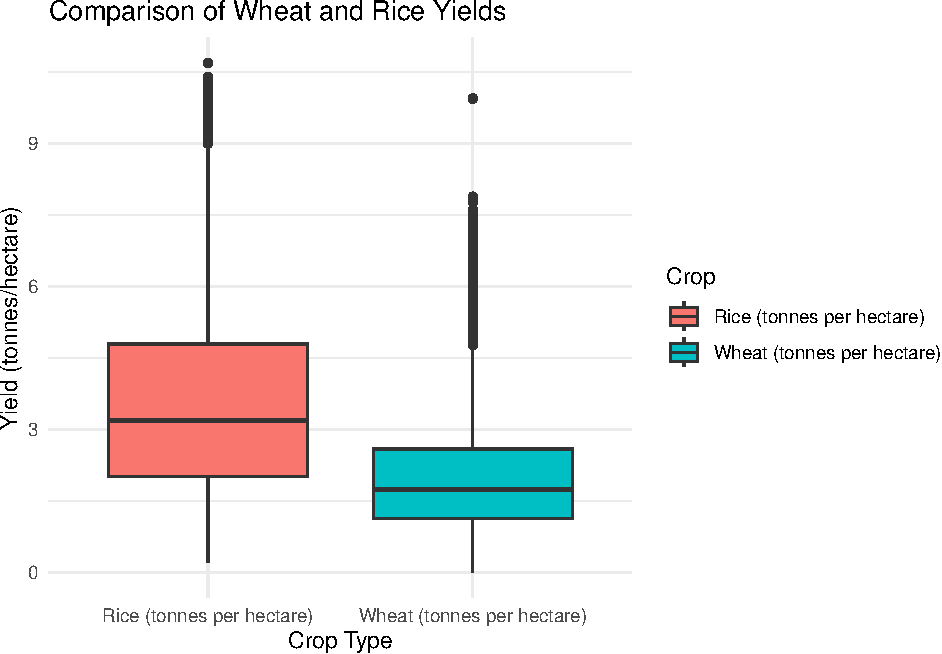
\includegraphics[keepaspectratio]{chapters/05-statistical-tests_files/figure-pdf/unnamed-chunk-4-1.pdf}}

\begin{Shaded}
\begin{Highlighting}[]
\CommentTok{\# Perform paired t{-}test using vectors directly}
\NormalTok{paired\_t\_test }\OtherTok{\textless{}{-}} \FunctionTok{t.test}\NormalTok{(}
\NormalTok{  paired\_data}\SpecialCharTok{$}\StringTok{\textasciigrave{}}\AttributeTok{Wheat (tonnes per hectare)}\StringTok{\textasciigrave{}}\NormalTok{, }
\NormalTok{  paired\_data}\SpecialCharTok{$}\StringTok{\textasciigrave{}}\AttributeTok{Rice (tonnes per hectare)}\StringTok{\textasciigrave{}}\NormalTok{, }
  \AttributeTok{paired =} \ConstantTok{TRUE}
\NormalTok{)}
\NormalTok{paired\_t\_test}
\end{Highlighting}
\end{Shaded}

\begin{verbatim}

    Paired t-test

data:  paired_data$`Wheat (tonnes per hectare)` and paired_data$`Rice (tonnes per hectare)`
t = -61.854, df = 5725, p-value < 2.2e-16
alternative hypothesis: true mean difference is not equal to 0
95 percent confidence interval:
 -1.565063 -1.468905
sample estimates:
mean difference 
      -1.516984 
\end{verbatim}

\subsection{Analysis of Variance
(ANOVA)}\label{analysis-of-variance-anova}

ANOVA is used to compare means among three or more independent groups.
Let's compare crop yields across different continents:

\begin{Shaded}
\begin{Highlighting}[]
\CommentTok{\# Create a mapping of countries to continents (simplified for demonstration)}
\NormalTok{continent\_mapping }\OtherTok{\textless{}{-}} \FunctionTok{tibble}\NormalTok{(}
  \AttributeTok{Entity =} \FunctionTok{c}\NormalTok{(}\StringTok{"United States"}\NormalTok{, }\StringTok{"Canada"}\NormalTok{, }\StringTok{"Mexico"}\NormalTok{, }
             \StringTok{"China"}\NormalTok{, }\StringTok{"India"}\NormalTok{, }\StringTok{"Japan"}\NormalTok{, }
             \StringTok{"Germany"}\NormalTok{, }\StringTok{"France"}\NormalTok{, }\StringTok{"United Kingdom"}\NormalTok{, }
             \StringTok{"Brazil"}\NormalTok{, }\StringTok{"Argentina"}\NormalTok{, }\StringTok{"Chile"}\NormalTok{,}
             \StringTok{"Egypt"}\NormalTok{, }\StringTok{"Nigeria"}\NormalTok{, }\StringTok{"South Africa"}\NormalTok{,}
             \StringTok{"Australia"}\NormalTok{, }\StringTok{"New Zealand"}\NormalTok{),}
  \AttributeTok{Continent =} \FunctionTok{c}\NormalTok{(}\FunctionTok{rep}\NormalTok{(}\StringTok{"North America"}\NormalTok{, }\DecValTok{3}\NormalTok{), }
                \FunctionTok{rep}\NormalTok{(}\StringTok{"Asia"}\NormalTok{, }\DecValTok{3}\NormalTok{), }
                \FunctionTok{rep}\NormalTok{(}\StringTok{"Europe"}\NormalTok{, }\DecValTok{3}\NormalTok{), }
                \FunctionTok{rep}\NormalTok{(}\StringTok{"South America"}\NormalTok{, }\DecValTok{3}\NormalTok{),}
                \FunctionTok{rep}\NormalTok{(}\StringTok{"Africa"}\NormalTok{, }\DecValTok{3}\NormalTok{),}
                \FunctionTok{rep}\NormalTok{(}\StringTok{"Oceania"}\NormalTok{, }\DecValTok{2}\NormalTok{))}
\NormalTok{)}

\CommentTok{\# Join with crop yields data}
\NormalTok{continental\_yields }\OtherTok{\textless{}{-}}\NormalTok{ crop\_yields }\SpecialCharTok{\%\textgreater{}\%}
  \FunctionTok{inner\_join}\NormalTok{(continent\_mapping, }\AttributeTok{by =} \StringTok{"Entity"}\NormalTok{) }\SpecialCharTok{\%\textgreater{}\%}
  \FunctionTok{filter}\NormalTok{(}\SpecialCharTok{!}\FunctionTok{is.na}\NormalTok{(}\StringTok{\textasciigrave{}}\AttributeTok{Wheat (tonnes per hectare)}\StringTok{\textasciigrave{}}\NormalTok{) }\SpecialCharTok{\&}\NormalTok{ Year }\SpecialCharTok{\textgreater{}=} \DecValTok{2000}\NormalTok{)}

\CommentTok{\# Visualize wheat yields by continent}
\FunctionTok{ggplot}\NormalTok{(continental\_yields, }\FunctionTok{aes}\NormalTok{(}\AttributeTok{x =}\NormalTok{ Continent, }\AttributeTok{y =} \StringTok{\textasciigrave{}}\AttributeTok{Wheat (tonnes per hectare)}\StringTok{\textasciigrave{}}\NormalTok{, }\AttributeTok{fill =}\NormalTok{ Continent)) }\SpecialCharTok{+}
  \FunctionTok{geom\_boxplot}\NormalTok{() }\SpecialCharTok{+}
  \FunctionTok{labs}\NormalTok{(}\AttributeTok{title =} \StringTok{"Wheat Yields by Continent (2000{-}present)"}\NormalTok{,}
       \AttributeTok{x =} \StringTok{"Continent"}\NormalTok{,}
       \AttributeTok{y =} \StringTok{"Wheat Yield (tonnes/hectare)"}\NormalTok{) }\SpecialCharTok{+}
  \FunctionTok{theme\_minimal}\NormalTok{() }\SpecialCharTok{+}
  \FunctionTok{theme}\NormalTok{(}\AttributeTok{axis.text.x =} \FunctionTok{element\_text}\NormalTok{(}\AttributeTok{angle =} \DecValTok{45}\NormalTok{, }\AttributeTok{hjust =} \DecValTok{1}\NormalTok{))}
\end{Highlighting}
\end{Shaded}

\pandocbounded{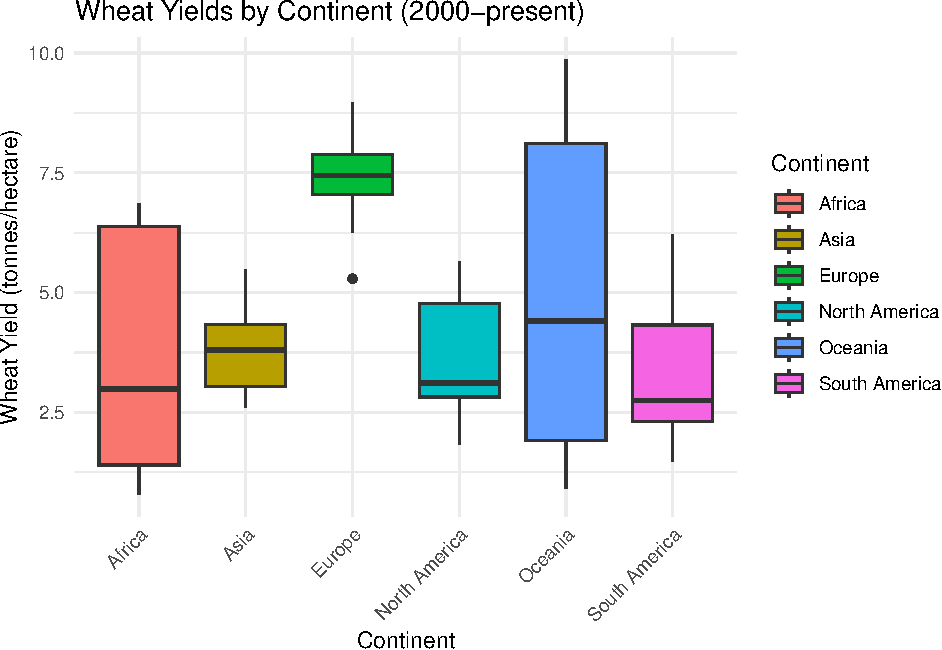
\includegraphics[keepaspectratio]{chapters/05-statistical-tests_files/figure-pdf/unnamed-chunk-5-1.pdf}}

\begin{Shaded}
\begin{Highlighting}[]
\CommentTok{\# Perform ANOVA}
\NormalTok{anova\_result }\OtherTok{\textless{}{-}} \FunctionTok{aov}\NormalTok{(}\StringTok{\textasciigrave{}}\AttributeTok{Wheat (tonnes per hectare)}\StringTok{\textasciigrave{}} \SpecialCharTok{\textasciitilde{}}\NormalTok{ Continent, }\AttributeTok{data =}\NormalTok{ continental\_yields)}
\FunctionTok{summary}\NormalTok{(anova\_result)}
\end{Highlighting}
\end{Shaded}

\begin{verbatim}
             Df Sum Sq Mean Sq F value Pr(>F)    
Continent     5  698.6  139.73   48.64 <2e-16 ***
Residuals   317  910.7    2.87                   
---
Signif. codes:  0 '***' 0.001 '**' 0.01 '*' 0.05 '.' 0.1 ' ' 1
\end{verbatim}

\begin{Shaded}
\begin{Highlighting}[]
\CommentTok{\# Post{-}hoc test to identify which groups differ}
\FunctionTok{TukeyHSD}\NormalTok{(anova\_result)}
\end{Highlighting}
\end{Shaded}

\begin{verbatim}
  Tukey multiple comparisons of means
    95% family-wise confidence level

Fit: aov(formula = `Wheat (tonnes per hectare)` ~ Continent, data = continental_yields)

$Continent
                                   diff         lwr        upr     p adj
Asia-Africa                  0.27759825 -0.63272412  1.1879206 0.9523916
Europe-Africa                3.89405789  2.98373553  4.8043803 0.0000000
North America-Africa         0.06069825 -0.84962412  0.9710206 0.9999646
Oceania-Africa               1.36844649  0.35067515  2.3862178 0.0019309
South America-Africa        -0.21777193 -1.12809429  0.6925504 0.9834279
Europe-Asia                  3.61645965  2.70613729  4.5267820 0.0000000
North America-Asia          -0.21690000 -1.12722236  0.6934224 0.9837237
Oceania-Asia                 1.09084825  0.07307691  2.1086196 0.0276496
South America-Asia          -0.49537018 -1.40569254  0.4149522 0.6253648
North America-Europe        -3.83335965 -4.74368201 -2.9230373 0.0000000
Oceania-Europe              -2.52561140 -3.54338274 -1.5078401 0.0000000
South America-Europe        -4.11182982 -5.02215219 -3.2015075 0.0000000
Oceania-North America        1.30774825  0.28997691  2.3255196 0.0036420
South America-North America -0.27847018 -1.18879254  0.6318522 0.9517629
South America-Oceania       -1.58621842 -2.60398976 -0.5684471 0.0001587
\end{verbatim}

\subsection{Non-Parametric
Alternatives}\label{non-parametric-alternatives}

\subsubsection{Mann-Whitney U Test}\label{mann-whitney-u-test}

The Mann-Whitney U test (also called Wilcoxon rank-sum test) is a
non-parametric alternative to the independent samples t-test:

\begin{Shaded}
\begin{Highlighting}[]
\CommentTok{\# Using the same time period groups as before}
\NormalTok{wilcox\_test }\OtherTok{\textless{}{-}} \FunctionTok{wilcox.test}\NormalTok{(}\StringTok{\textasciigrave{}}\AttributeTok{Wheat (tonnes per hectare)}\StringTok{\textasciigrave{}} \SpecialCharTok{\textasciitilde{}}\NormalTok{ period, }\AttributeTok{data =}\NormalTok{ crop\_yields\_grouped)}
\NormalTok{wilcox\_test}
\end{Highlighting}
\end{Shaded}

\begin{verbatim}

    Wilcoxon rank sum test with continuity correction

data:  Wheat (tonnes per hectare) by period
W = 5031268, p-value < 2.2e-16
alternative hypothesis: true location shift is not equal to 0
\end{verbatim}

\subsubsection{Kruskal-Wallis Test}\label{kruskal-wallis-test}

The Kruskal-Wallis test is a non-parametric alternative to ANOVA:

\begin{Shaded}
\begin{Highlighting}[]
\CommentTok{\# Using the same continental data as before}
\NormalTok{kruskal\_result }\OtherTok{\textless{}{-}} \FunctionTok{kruskal.test}\NormalTok{(}\StringTok{\textasciigrave{}}\AttributeTok{Wheat (tonnes per hectare)}\StringTok{\textasciigrave{}} \SpecialCharTok{\textasciitilde{}}\NormalTok{ Continent, }\AttributeTok{data =}\NormalTok{ continental\_yields)}
\NormalTok{kruskal\_result}
\end{Highlighting}
\end{Shaded}

\begin{verbatim}

    Kruskal-Wallis rank sum test

data:  Wheat (tonnes per hectare) by Continent
Kruskal-Wallis chi-squared = 120.17, df = 5, p-value < 2.2e-16
\end{verbatim}

\begin{Shaded}
\begin{Highlighting}[]
\CommentTok{\# Post{-}hoc test for Kruskal{-}Wallis}
\ControlFlowTok{if}\NormalTok{(}\FunctionTok{requireNamespace}\NormalTok{(}\StringTok{"dunn.test"}\NormalTok{, }\AttributeTok{quietly =} \ConstantTok{TRUE}\NormalTok{)) \{}
  \FunctionTok{library}\NormalTok{(dunn.test)}
  \FunctionTok{dunn.test}\NormalTok{(continental\_yields}\SpecialCharTok{$}\StringTok{\textasciigrave{}}\AttributeTok{Wheat (tonnes per hectare)}\StringTok{\textasciigrave{}}\NormalTok{, continental\_yields}\SpecialCharTok{$}\NormalTok{Continent, }\AttributeTok{method =} \StringTok{"bonferroni"}\NormalTok{)}
\NormalTok{\} }\ControlFlowTok{else}\NormalTok{ \{}
  \CommentTok{\# Alternative: pairwise Wilcoxon tests}
  \FunctionTok{pairwise.wilcox.test}\NormalTok{(continental\_yields}\SpecialCharTok{$}\StringTok{\textasciigrave{}}\AttributeTok{Wheat (tonnes per hectare)}\StringTok{\textasciigrave{}}\NormalTok{, continental\_yields}\SpecialCharTok{$}\NormalTok{Continent, }
                       \AttributeTok{p.adjust.method =} \StringTok{"bonferroni"}\NormalTok{)}
\NormalTok{\}}
\end{Highlighting}
\end{Shaded}

\begin{verbatim}
  Kruskal-Wallis rank sum test

data: x and group
Kruskal-Wallis chi-squared = 120.1715, df = 5, p-value = 0

                           Comparison of x by group                            
                                 (Bonferroni)                                  
Col Mean-|
Row Mean |     Africa       Asia     Europe   North Am    Oceania
---------+-------------------------------------------------------
    Asia |  -1.814776
         |     0.5217
         |
  Europe |  -9.079400  -7.264623
         |    0.0000*    0.0000*
         |
North Am |  -0.948758   0.866018   8.130641
         |     1.0000     1.0000    0.0000*
         |
 Oceania |  -2.181366  -0.558180   5.939496  -1.332770
         |     0.2187     1.0000    0.0000*     1.0000
         |
South Am |   0.300874   2.115651   9.380275   1.249633   2.450476
         |     1.0000     0.2578    0.0000*     1.0000     0.1070

alpha = 0.05
Reject Ho if p <= alpha/2
\end{verbatim}

\section{Tests for Relationships}\label{tests-for-relationships}

\subsection{Correlation Analysis}\label{correlation-analysis-1}

\subsubsection{Pearson Correlation}\label{pearson-correlation}

Pearson correlation measures the linear relationship between two
continuous variables:

\begin{Shaded}
\begin{Highlighting}[]
\CommentTok{\# Examine correlation between wheat and maize yields}
\NormalTok{crop\_correlation }\OtherTok{\textless{}{-}}\NormalTok{ crop\_yields }\SpecialCharTok{\%\textgreater{}\%}
  \FunctionTok{filter}\NormalTok{(}\SpecialCharTok{!}\FunctionTok{is.na}\NormalTok{(}\StringTok{\textasciigrave{}}\AttributeTok{Wheat (tonnes per hectare)}\StringTok{\textasciigrave{}}\NormalTok{) }\SpecialCharTok{\&} \SpecialCharTok{!}\FunctionTok{is.na}\NormalTok{(}\StringTok{\textasciigrave{}}\AttributeTok{Maize (tonnes per hectare)}\StringTok{\textasciigrave{}}\NormalTok{)) }\SpecialCharTok{\%\textgreater{}\%}
  \FunctionTok{select}\NormalTok{(Entity, Year, }\StringTok{\textasciigrave{}}\AttributeTok{Wheat (tonnes per hectare)}\StringTok{\textasciigrave{}}\NormalTok{, }\StringTok{\textasciigrave{}}\AttributeTok{Maize (tonnes per hectare)}\StringTok{\textasciigrave{}}\NormalTok{)}

\CommentTok{\# Visualize the relationship}
\FunctionTok{ggplot}\NormalTok{(crop\_correlation, }\FunctionTok{aes}\NormalTok{(}\AttributeTok{x =} \StringTok{\textasciigrave{}}\AttributeTok{Wheat (tonnes per hectare)}\StringTok{\textasciigrave{}}\NormalTok{, }\AttributeTok{y =} \StringTok{\textasciigrave{}}\AttributeTok{Maize (tonnes per hectare)}\StringTok{\textasciigrave{}}\NormalTok{)) }\SpecialCharTok{+}
  \FunctionTok{geom\_point}\NormalTok{(}\AttributeTok{alpha =} \FloatTok{0.5}\NormalTok{) }\SpecialCharTok{+}
  \FunctionTok{geom\_smooth}\NormalTok{(}\AttributeTok{method =} \StringTok{"lm"}\NormalTok{, }\AttributeTok{se =} \ConstantTok{TRUE}\NormalTok{, }\AttributeTok{color =} \StringTok{"blue"}\NormalTok{) }\SpecialCharTok{+}
  \FunctionTok{labs}\NormalTok{(}\AttributeTok{title =} \StringTok{"Relationship Between Wheat and Maize Yields"}\NormalTok{,}
       \AttributeTok{x =} \StringTok{"Wheat Yield (tonnes per hectare)"}\NormalTok{,}
       \AttributeTok{y =} \StringTok{"Maize Yield (tonnes per hectare)"}\NormalTok{) }\SpecialCharTok{+}
  \FunctionTok{theme\_minimal}\NormalTok{()}
\end{Highlighting}
\end{Shaded}

\pandocbounded{\includegraphics[keepaspectratio]{chapters/05-statistical-tests_files/figure-pdf/unnamed-chunk-8-1.pdf}}

\begin{Shaded}
\begin{Highlighting}[]
\CommentTok{\# Calculate Pearson correlation}
\NormalTok{cor\_result }\OtherTok{\textless{}{-}} \FunctionTok{cor.test}\NormalTok{(crop\_correlation}\SpecialCharTok{$}\StringTok{\textasciigrave{}}\AttributeTok{Wheat (tonnes per hectare)}\StringTok{\textasciigrave{}}\NormalTok{, crop\_correlation}\SpecialCharTok{$}\StringTok{\textasciigrave{}}\AttributeTok{Maize (tonnes per hectare)}\StringTok{\textasciigrave{}}\NormalTok{, }\AttributeTok{method =} \StringTok{"pearson"}\NormalTok{)}
\NormalTok{cor\_result}
\end{Highlighting}
\end{Shaded}

\begin{verbatim}

    Pearson's product-moment correlation

data:  crop_correlation$`Wheat (tonnes per hectare)` and crop_correlation$`Maize (tonnes per hectare)`
t = 49.748, df = 7378, p-value < 2.2e-16
alternative hypothesis: true correlation is not equal to 0
95 percent confidence interval:
 0.4838956 0.5180698
sample estimates:
      cor 
0.5011781 
\end{verbatim}

\subsubsection{Spearman Correlation}\label{spearman-correlation}

Spearman correlation is a non-parametric measure of rank correlation:

\begin{Shaded}
\begin{Highlighting}[]
\CommentTok{\# Calculate Spearman correlation}
\NormalTok{spearman\_result }\OtherTok{\textless{}{-}} \FunctionTok{cor.test}\NormalTok{(crop\_correlation}\SpecialCharTok{$}\StringTok{\textasciigrave{}}\AttributeTok{Wheat (tonnes per hectare)}\StringTok{\textasciigrave{}}\NormalTok{, crop\_correlation}\SpecialCharTok{$}\StringTok{\textasciigrave{}}\AttributeTok{Maize (tonnes per hectare)}\StringTok{\textasciigrave{}}\NormalTok{, }\AttributeTok{method =} \StringTok{"spearman"}\NormalTok{)}
\NormalTok{spearman\_result}
\end{Highlighting}
\end{Shaded}

\begin{verbatim}

    Spearman's rank correlation rho

data:  crop_correlation$`Wheat (tonnes per hectare)` and crop_correlation$`Maize (tonnes per hectare)`
S = 2.4618e+10, p-value < 2.2e-16
alternative hypothesis: true rho is not equal to 0
sample estimates:
      rho 
0.6325152 
\end{verbatim}

\subsection{Regression Analysis}\label{regression-analysis}

\subsubsection{Linear Regression}\label{linear-regression}

Linear regression models the relationship between a dependent variable
and one or more independent variables:

\begin{Shaded}
\begin{Highlighting}[]
\CommentTok{\# Create a dataset with year as predictor for wheat yields}
\NormalTok{time\_series\_data }\OtherTok{\textless{}{-}}\NormalTok{ crop\_yields }\SpecialCharTok{\%\textgreater{}\%}
  \FunctionTok{filter}\NormalTok{(Entity }\SpecialCharTok{==} \StringTok{"United States"} \SpecialCharTok{\&} \SpecialCharTok{!}\FunctionTok{is.na}\NormalTok{(}\StringTok{\textasciigrave{}}\AttributeTok{Wheat (tonnes per hectare)}\StringTok{\textasciigrave{}}\NormalTok{)) }\SpecialCharTok{\%\textgreater{}\%}
  \FunctionTok{arrange}\NormalTok{(Year)}

\CommentTok{\# Visualize the trend}
\FunctionTok{ggplot}\NormalTok{(time\_series\_data, }\FunctionTok{aes}\NormalTok{(}\AttributeTok{x =}\NormalTok{ Year, }\AttributeTok{y =} \StringTok{\textasciigrave{}}\AttributeTok{Wheat (tonnes per hectare)}\StringTok{\textasciigrave{}}\NormalTok{)) }\SpecialCharTok{+}
  \FunctionTok{geom\_point}\NormalTok{() }\SpecialCharTok{+}
  \FunctionTok{geom\_smooth}\NormalTok{(}\AttributeTok{method =} \StringTok{"lm"}\NormalTok{, }\AttributeTok{se =} \ConstantTok{TRUE}\NormalTok{, }\AttributeTok{color =} \StringTok{"blue"}\NormalTok{) }\SpecialCharTok{+}
  \FunctionTok{labs}\NormalTok{(}\AttributeTok{title =} \StringTok{"Wheat Yield Trends in the United States"}\NormalTok{,}
       \AttributeTok{x =} \StringTok{"Year"}\NormalTok{,}
       \AttributeTok{y =} \StringTok{"Wheat Yield (tonnes/hectare)"}\NormalTok{) }\SpecialCharTok{+}
  \FunctionTok{theme\_minimal}\NormalTok{()}
\end{Highlighting}
\end{Shaded}

\pandocbounded{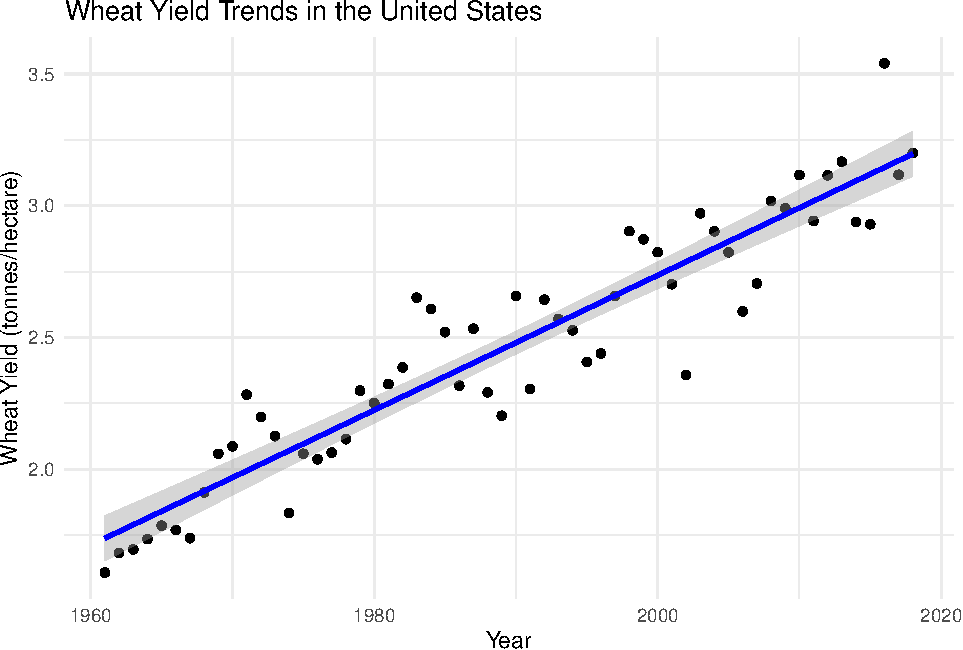
\includegraphics[keepaspectratio]{chapters/05-statistical-tests_files/figure-pdf/unnamed-chunk-10-1.pdf}}

\begin{Shaded}
\begin{Highlighting}[]
\CommentTok{\# Perform linear regression}
\NormalTok{lm\_model }\OtherTok{\textless{}{-}} \FunctionTok{lm}\NormalTok{(}\StringTok{\textasciigrave{}}\AttributeTok{Wheat (tonnes per hectare)}\StringTok{\textasciigrave{}} \SpecialCharTok{\textasciitilde{}}\NormalTok{ Year, }\AttributeTok{data =}\NormalTok{ time\_series\_data)}
\FunctionTok{summary}\NormalTok{(lm\_model)}
\end{Highlighting}
\end{Shaded}

\begin{verbatim}

Call:
lm(formula = `Wheat (tonnes per hectare)` ~ Year, data = time_series_data)

Residuals:
     Min       1Q   Median       3Q      Max 
-0.43042 -0.09139 -0.00340  0.11184  0.39526 

Coefficients:
              Estimate Std. Error t value Pr(>|t|)    
(Intercept) -48.465987   2.571017  -18.85   <2e-16 ***
Year          0.025601   0.001292   19.81   <2e-16 ***
---
Signif. codes:  0 '***' 0.001 '**' 0.01 '*' 0.05 '.' 0.1 ' ' 1

Residual standard error: 0.1648 on 56 degrees of freedom
Multiple R-squared:  0.8751,    Adjusted R-squared:  0.8729 
F-statistic: 392.5 on 1 and 56 DF,  p-value: < 2.2e-16
\end{verbatim}

\begin{Shaded}
\begin{Highlighting}[]
\CommentTok{\# Check assumptions}
\FunctionTok{par}\NormalTok{(}\AttributeTok{mfrow =} \FunctionTok{c}\NormalTok{(}\DecValTok{2}\NormalTok{, }\DecValTok{2}\NormalTok{))}
\FunctionTok{plot}\NormalTok{(lm\_model)}
\end{Highlighting}
\end{Shaded}

\pandocbounded{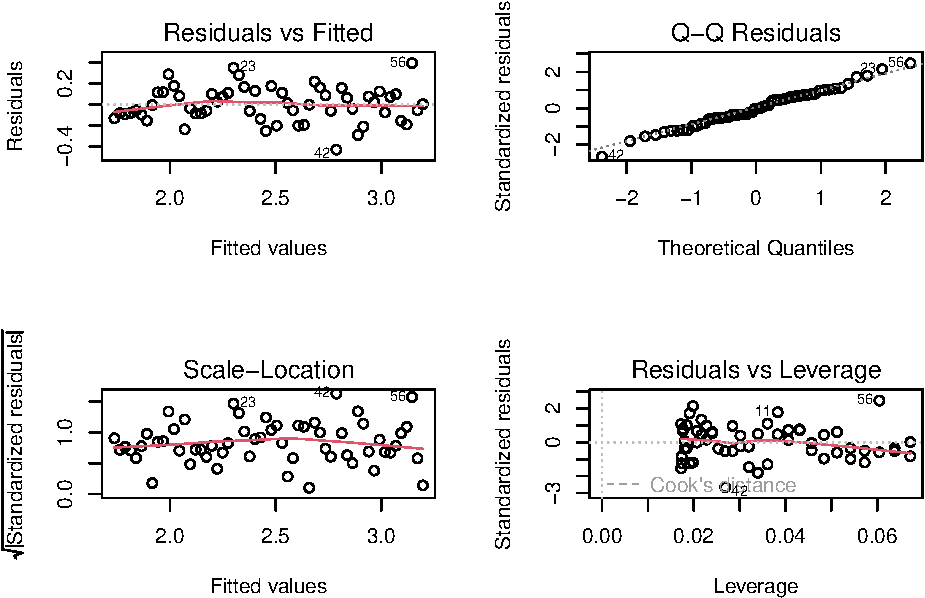
\includegraphics[keepaspectratio]{chapters/05-statistical-tests_files/figure-pdf/unnamed-chunk-10-2.pdf}}

\subsubsection{Multiple Regression}\label{multiple-regression}

Multiple regression includes more than one predictor variable:

\begin{Shaded}
\begin{Highlighting}[]
\CommentTok{\# Create a dataset with multiple predictors}
\NormalTok{multi\_crop\_data }\OtherTok{\textless{}{-}}\NormalTok{ crop\_yields }\SpecialCharTok{\%\textgreater{}\%}
  \FunctionTok{filter}\NormalTok{(}\SpecialCharTok{!}\FunctionTok{is.na}\NormalTok{(}\StringTok{\textasciigrave{}}\AttributeTok{Wheat (tonnes per hectare)}\StringTok{\textasciigrave{}}\NormalTok{) }\SpecialCharTok{\&} \SpecialCharTok{!}\FunctionTok{is.na}\NormalTok{(}\StringTok{\textasciigrave{}}\AttributeTok{Rice (tonnes per hectare)}\StringTok{\textasciigrave{}}\NormalTok{) }\SpecialCharTok{\&} \SpecialCharTok{!}\FunctionTok{is.na}\NormalTok{(}\StringTok{\textasciigrave{}}\AttributeTok{Maize (tonnes per hectare)}\StringTok{\textasciigrave{}}\NormalTok{)) }\SpecialCharTok{\%\textgreater{}\%}
  \FunctionTok{select}\NormalTok{(Entity, Year, }\StringTok{\textasciigrave{}}\AttributeTok{Wheat (tonnes per hectare)}\StringTok{\textasciigrave{}}\NormalTok{, }\StringTok{\textasciigrave{}}\AttributeTok{Rice (tonnes per hectare)}\StringTok{\textasciigrave{}}\NormalTok{, }\StringTok{\textasciigrave{}}\AttributeTok{Maize (tonnes per hectare)}\StringTok{\textasciigrave{}}\NormalTok{)}

\CommentTok{\# Perform multiple regression}
\NormalTok{multi\_model }\OtherTok{\textless{}{-}} \FunctionTok{lm}\NormalTok{(}\StringTok{\textasciigrave{}}\AttributeTok{Wheat (tonnes per hectare)}\StringTok{\textasciigrave{}} \SpecialCharTok{\textasciitilde{}} \StringTok{\textasciigrave{}}\AttributeTok{Rice (tonnes per hectare)}\StringTok{\textasciigrave{}} \SpecialCharTok{+} \StringTok{\textasciigrave{}}\AttributeTok{Maize (tonnes per hectare)}\StringTok{\textasciigrave{}} \SpecialCharTok{+}\NormalTok{ Year, }\AttributeTok{data =}\NormalTok{ multi\_crop\_data)}
\FunctionTok{summary}\NormalTok{(multi\_model)}
\end{Highlighting}
\end{Shaded}

\begin{verbatim}

Call:
lm(formula = `Wheat (tonnes per hectare)` ~ `Rice (tonnes per hectare)` + 
    `Maize (tonnes per hectare)` + Year, data = multi_crop_data)

Residuals:
    Min      1Q  Median      3Q     Max 
-2.7029 -0.6135 -0.2079  0.3877  7.8709 

Coefficients:
                               Estimate Std. Error t value Pr(>|t|)    
(Intercept)                  -2.161e+01  1.776e+00 -12.171   <2e-16 ***
`Rice (tonnes per hectare)`  -5.426e-03  9.720e-03  -0.558    0.577    
`Maize (tonnes per hectare)`  2.790e-01  8.512e-03  32.776   <2e-16 ***
Year                          1.148e-02  8.965e-04  12.810   <2e-16 ***
---
Signif. codes:  0 '***' 0.001 '**' 0.01 '*' 0.05 '.' 0.1 ' ' 1

Residual standard error: 1.025 on 5722 degrees of freedom
Multiple R-squared:  0.3411,    Adjusted R-squared:  0.3407 
F-statistic: 987.2 on 3 and 5722 DF,  p-value: < 2.2e-16
\end{verbatim}

\section{Tests for Categorical Data}\label{tests-for-categorical-data}

\subsection{Chi-Square Test}\label{chi-square-test}

The Chi-Square test examines the association between categorical
variables. Let's use our biodiversity dataset:

\begin{Shaded}
\begin{Highlighting}[]
\CommentTok{\# Load the biodiversity dataset}
\NormalTok{plants }\OtherTok{\textless{}{-}} \FunctionTok{read\_csv}\NormalTok{(}\StringTok{"../data/ecology/biodiversity.csv"}\NormalTok{)}

\CommentTok{\# Create a contingency table of red list categories by plant group}
\ControlFlowTok{if}\NormalTok{(}\StringTok{"red\_list\_category"} \SpecialCharTok{\%in\%} \FunctionTok{colnames}\NormalTok{(plants) }\SpecialCharTok{\&} \StringTok{"group"} \SpecialCharTok{\%in\%} \FunctionTok{colnames}\NormalTok{(plants)) \{}
  \CommentTok{\# Create a contingency table}
\NormalTok{  contingency\_table }\OtherTok{\textless{}{-}} \FunctionTok{table}\NormalTok{(plants}\SpecialCharTok{$}\NormalTok{red\_list\_category, plants}\SpecialCharTok{$}\NormalTok{group)}
  
  \CommentTok{\# View the table}
\NormalTok{  contingency\_table}
  
  \CommentTok{\# Perform Chi{-}Square test}
\NormalTok{  chi\_sq\_result }\OtherTok{\textless{}{-}} \FunctionTok{chisq.test}\NormalTok{(contingency\_table)}
\NormalTok{  chi\_sq\_result}
  
  \CommentTok{\# Examine residuals to understand the pattern of association}
\NormalTok{  chi\_sq\_result}\SpecialCharTok{$}\NormalTok{residuals}
\NormalTok{\} }\ControlFlowTok{else}\NormalTok{ \{}
  \CommentTok{\# If the expected columns don\textquotesingle{}t exist, create a demonstration with available data}
  \FunctionTok{message}\NormalTok{(}\StringTok{"Required columns not found. Creating a demonstration with available columns."}\NormalTok{)}
  
  \CommentTok{\# Identify categorical columns}
\NormalTok{  categorical\_cols }\OtherTok{\textless{}{-}} \FunctionTok{sapply}\NormalTok{(plants, }\ControlFlowTok{function}\NormalTok{(x) }\FunctionTok{is.character}\NormalTok{(x) }\SpecialCharTok{||} \FunctionTok{is.factor}\NormalTok{(x))}
\NormalTok{  cat\_col\_names }\OtherTok{\textless{}{-}} \FunctionTok{names}\NormalTok{(plants)[categorical\_cols]}
  
  \ControlFlowTok{if}\NormalTok{(}\FunctionTok{length}\NormalTok{(cat\_col\_names) }\SpecialCharTok{\textgreater{}=} \DecValTok{2}\NormalTok{) \{}
    \CommentTok{\# Select the first two categorical columns}
\NormalTok{    col1 }\OtherTok{\textless{}{-}}\NormalTok{ cat\_col\_names[}\DecValTok{1}\NormalTok{]}
\NormalTok{    col2 }\OtherTok{\textless{}{-}}\NormalTok{ cat\_col\_names[}\DecValTok{2}\NormalTok{]}
    
    \CommentTok{\# Create a contingency table}
\NormalTok{    contingency\_table }\OtherTok{\textless{}{-}} \FunctionTok{table}\NormalTok{(plants[[col1]], plants[[col2]])}
    
    \CommentTok{\# View the table}
    \FunctionTok{print}\NormalTok{(}\FunctionTok{paste}\NormalTok{(}\StringTok{"Contingency table of"}\NormalTok{, col1, }\StringTok{"by"}\NormalTok{, col2))}
    \FunctionTok{print}\NormalTok{(contingency\_table)}
    
    \CommentTok{\# Perform Chi{-}Square test if appropriate}
    \ControlFlowTok{if}\NormalTok{(}\FunctionTok{min}\NormalTok{(}\FunctionTok{dim}\NormalTok{(contingency\_table)) }\SpecialCharTok{\textgreater{}} \DecValTok{1} \SpecialCharTok{\&\&} \FunctionTok{sum}\NormalTok{(contingency\_table) }\SpecialCharTok{\textgreater{}} \DecValTok{0}\NormalTok{) \{}
\NormalTok{      chi\_sq\_result }\OtherTok{\textless{}{-}} \FunctionTok{chisq.test}\NormalTok{(contingency\_table, }\AttributeTok{simulate.p.value =} \ConstantTok{TRUE}\NormalTok{)}
      \FunctionTok{print}\NormalTok{(chi\_sq\_result)}
\NormalTok{    \} }\ControlFlowTok{else}\NormalTok{ \{}
      \FunctionTok{message}\NormalTok{(}\StringTok{"Contingency table not suitable for Chi{-}Square test."}\NormalTok{)}
\NormalTok{    \}}
\NormalTok{  \} }\ControlFlowTok{else}\NormalTok{ \{}
    \FunctionTok{message}\NormalTok{(}\StringTok{"Not enough categorical columns found for Chi{-}Square test demonstration."}\NormalTok{)}
\NormalTok{  \}}
\NormalTok{\}}
\end{Highlighting}
\end{Shaded}

\begin{verbatim}
                     
                            Algae     Conifer       Cycad Ferns and Allies
  Extinct              0.24140394  0.13937463 -1.12198510       0.20517186
  Extinct in the Wild -0.62449980 -0.36055513  2.90251880      -0.53076923
                     
                      Flowering Plant      Mosses
  Extinct                  0.06076242  0.27874926
  Extinct in the Wild     -0.15718930 -0.72111026
\end{verbatim}

\section{Tests for Trends and Time
Series}\label{tests-for-trends-and-time-series}

\subsection{Time Series Analysis}\label{time-series-analysis}

Time series analysis examines data collected over time to identify
patterns, trends, and seasonal effects:

\begin{Shaded}
\begin{Highlighting}[]
\CommentTok{\# Create a time series of wheat yields for a specific country}
\NormalTok{us\_wheat }\OtherTok{\textless{}{-}}\NormalTok{ crop\_yields }\SpecialCharTok{\%\textgreater{}\%}
  \FunctionTok{filter}\NormalTok{(Entity }\SpecialCharTok{==} \StringTok{"United States"} \SpecialCharTok{\&} \SpecialCharTok{!}\FunctionTok{is.na}\NormalTok{(}\StringTok{\textasciigrave{}}\AttributeTok{Wheat (tonnes per hectare)}\StringTok{\textasciigrave{}}\NormalTok{)) }\SpecialCharTok{\%\textgreater{}\%}
  \FunctionTok{arrange}\NormalTok{(Year)}

\CommentTok{\# Convert to time series object}
\ControlFlowTok{if}\NormalTok{(}\FunctionTok{requireNamespace}\NormalTok{(}\StringTok{"zoo"}\NormalTok{, }\AttributeTok{quietly =} \ConstantTok{TRUE}\NormalTok{)) \{}
  \FunctionTok{library}\NormalTok{(zoo)}
\NormalTok{  wheat\_ts }\OtherTok{\textless{}{-}} \FunctionTok{zoo}\NormalTok{(us\_wheat}\SpecialCharTok{$}\StringTok{\textasciigrave{}}\AttributeTok{Wheat (tonnes per hectare)}\StringTok{\textasciigrave{}}\NormalTok{, us\_wheat}\SpecialCharTok{$}\NormalTok{Year)}
  
  \CommentTok{\# Plot the time series}
  \FunctionTok{plot}\NormalTok{(wheat\_ts, }\AttributeTok{main =} \StringTok{"US Wheat Yields Over Time"}\NormalTok{,}
       \AttributeTok{xlab =} \StringTok{"Year"}\NormalTok{, }\AttributeTok{ylab =} \StringTok{"Wheat Yield (tonnes/hectare)"}\NormalTok{)}
  
  \CommentTok{\# Add trend line}
  \FunctionTok{lines}\NormalTok{(}\FunctionTok{lowess}\NormalTok{(us\_wheat}\SpecialCharTok{$}\NormalTok{Year, us\_wheat}\SpecialCharTok{$}\StringTok{\textasciigrave{}}\AttributeTok{Wheat (tonnes per hectare)}\StringTok{\textasciigrave{}}\NormalTok{), }\AttributeTok{col =} \StringTok{"red"}\NormalTok{, }\AttributeTok{lwd =} \DecValTok{2}\NormalTok{)}
\NormalTok{\} }\ControlFlowTok{else}\NormalTok{ \{}
  \CommentTok{\# Basic plot if zoo package is not available}
  \FunctionTok{plot}\NormalTok{(us\_wheat}\SpecialCharTok{$}\NormalTok{Year, us\_wheat}\SpecialCharTok{$}\StringTok{\textasciigrave{}}\AttributeTok{Wheat (tonnes per hectare)}\StringTok{\textasciigrave{}}\NormalTok{, }\AttributeTok{type =} \StringTok{"l"}\NormalTok{,}
       \AttributeTok{main =} \StringTok{"US Wheat Yields Over Time"}\NormalTok{,}
       \AttributeTok{xlab =} \StringTok{"Year"}\NormalTok{, }\AttributeTok{ylab =} \StringTok{"Wheat Yield (tonnes per hectare)"}\NormalTok{)}
  
  \CommentTok{\# Add trend line}
  \FunctionTok{lines}\NormalTok{(}\FunctionTok{lowess}\NormalTok{(us\_wheat}\SpecialCharTok{$}\NormalTok{Year, us\_wheat}\SpecialCharTok{$}\StringTok{\textasciigrave{}}\AttributeTok{Wheat (tonnes per hectare)}\StringTok{\textasciigrave{}}\NormalTok{), }\AttributeTok{col =} \StringTok{"red"}\NormalTok{, }\AttributeTok{lwd =} \DecValTok{2}\NormalTok{)}
\NormalTok{\}}
\end{Highlighting}
\end{Shaded}

\pandocbounded{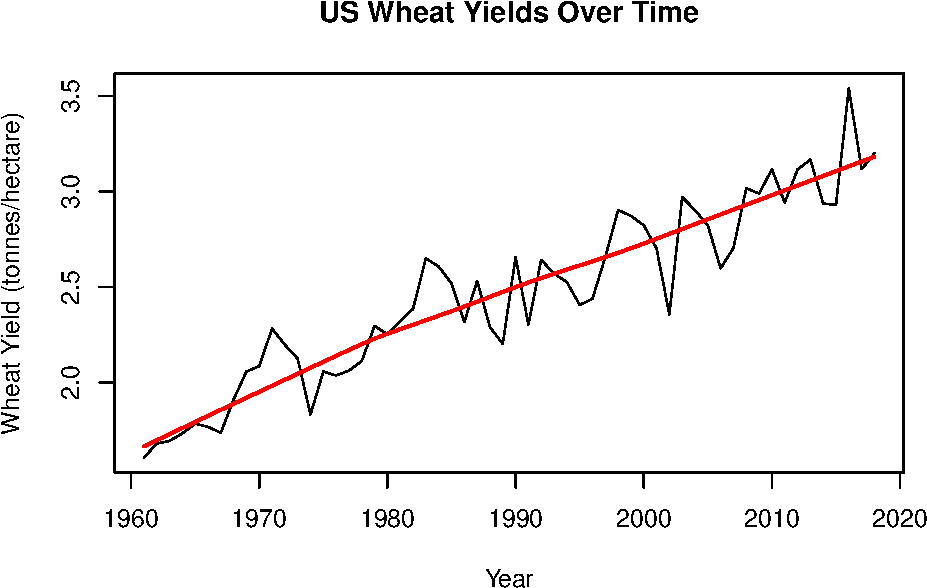
\includegraphics[keepaspectratio]{chapters/05-statistical-tests_files/figure-pdf/unnamed-chunk-13-1.pdf}}

\subsection{Mann-Kendall Trend Test}\label{mann-kendall-trend-test}

The Mann-Kendall test is a non-parametric test for identifying trends in
time series data:

\begin{Shaded}
\begin{Highlighting}[]
\CommentTok{\# Perform Mann{-}Kendall trend test}
\ControlFlowTok{if}\NormalTok{(}\FunctionTok{requireNamespace}\NormalTok{(}\StringTok{"Kendall"}\NormalTok{, }\AttributeTok{quietly =} \ConstantTok{TRUE}\NormalTok{)) \{}
  \FunctionTok{library}\NormalTok{(Kendall)}
\NormalTok{  mk\_test }\OtherTok{\textless{}{-}}\NormalTok{ Kendall}\SpecialCharTok{::}\FunctionTok{MannKendall}\NormalTok{(us\_wheat}\SpecialCharTok{$}\StringTok{\textasciigrave{}}\AttributeTok{Wheat (tonnes per hectare)}\StringTok{\textasciigrave{}}\NormalTok{)}
  \FunctionTok{print}\NormalTok{(mk\_test)}
\NormalTok{\} }\ControlFlowTok{else}\NormalTok{ \{}
  \FunctionTok{message}\NormalTok{(}\StringTok{"The Kendall package is not installed. Install it with install.packages(\textquotesingle{}Kendall\textquotesingle{}) to run the Mann{-}Kendall trend test."}\NormalTok{)}
\NormalTok{\}}
\end{Highlighting}
\end{Shaded}

\begin{verbatim}
tau = 0.798, 2-sided pvalue =< 2.22e-16
\end{verbatim}

\section{Summary}\label{summary-4}

This chapter has demonstrated a variety of statistical tests using real
agricultural and biodiversity datasets. We've covered:

\begin{enumerate}
\def\labelenumi{\arabic{enumi}.}
\tightlist
\item
  \textbf{Tests for comparing groups}:

  \begin{itemize}
  \tightlist
  \item
    t-tests for comparing two groups
  \item
    ANOVA for comparing multiple groups
  \item
    Non-parametric alternatives when data doesn't meet parametric
    assumptions
  \end{itemize}
\item
  \textbf{Tests for relationships}:

  \begin{itemize}
  \tightlist
  \item
    Correlation analysis to measure the strength of relationships
  \item
    Regression analysis to model relationships between variables
  \end{itemize}
\item
  \textbf{Tests for categorical data}:

  \begin{itemize}
  \tightlist
  \item
    Chi-Square test for examining associations between categorical
    variables
  \end{itemize}
\item
  \textbf{Tests for time series data}:

  \begin{itemize}
  \tightlist
  \item
    Time series analysis for identifying patterns over time
  \item
    Mann-Kendall test for detecting trends
  \end{itemize}
\end{enumerate}

When conducting statistical tests, remember to: - Clearly define your
research question - Check if your data meets the assumptions of the test
- Choose the appropriate test based on your data type and research
question - Interpret results in the context of your research question -
Consider the practical significance, not just statistical significance

\section{Exercises}\label{exercises-4}

\begin{enumerate}
\def\labelenumi{\arabic{enumi}.}
\item
  Using the crop yield dataset, compare maize yields between continents
  using both ANOVA and the Kruskal-Wallis test. Which is more
  appropriate and why?
\item
  Examine the relationship between potato and rice yields using
  correlation analysis. Calculate both Pearson and Spearman correlations
  and explain which is more appropriate.
\item
  Using the biodiversity dataset, investigate whether there's an
  association between conservation status and another categorical
  variable of your choice.
\item
  Perform a time series analysis of wheat yields for China and compare
  the trend with that of the United States.
\item
  Using the animal dataset (\texttt{../data/entomology/insects.csv}),
  compare two groups using an appropriate statistical test.
\item
  Create a multiple regression model to predict coffee quality scores
  using the coffee economics dataset
  (\texttt{../data/economics/economic.csv}).
\end{enumerate}

\section{Enhanced Statistical Tests
Chapter}\label{enhanced-statistical-tests-chapter}

The enhanced visualizations and tables for this chapter are available in
a separate file to ensure compatibility with the book rendering process.

\part{Data Visualization}

\chapter{Data Visualization}\label{data-visualization-1}

\section{Introduction}\label{introduction-4}

Data visualization is a crucial skill for communicating scientific
findings effectively. In this chapter, you will:

\begin{itemize}
\tightlist
\item
  Learn various data visualization techniques
\item
  Gain expertise in creating informative graphs and plots
\item
  Understand the role of visualization in conveying insights clearly in
  natural sciences
\end{itemize}

\section{The Importance of Data
Visualization}\label{the-importance-of-data-visualization}

\subsection{Why Data Visualization
Matters}\label{why-data-visualization-matters}

Data visualization plays a pivotal role in natural sciences research for
several reasons:

\begin{enumerate}
\def\labelenumi{\arabic{enumi}.}
\item
  \textbf{Pattern Recognition:} Visualizations make it easier to
  identify patterns, trends, and anomalies in data. This can reveal
  phenomena like population fluctuations, species distributions, or the
  impact of environmental factors.
\item
  \textbf{Communication:} Effective visualizations simplify complex
  scientific concepts, enabling researchers to convey findings to both
  expert and non-expert audiences. This is particularly valuable when
  sharing results with policymakers, stakeholders, or the general
  public.
\item
  \textbf{Hypothesis Testing:} Visualizations assist in formulating and
  testing scientific hypotheses. Researchers can visually explore data
  distributions, relationships, and spatial patterns, which informs the
  design of hypothesis tests.
\item
  \textbf{Decision-Making:} Visualizations aid in making informed
  decisions about conservation and management strategies. For example,
  they can illustrate the effects of different interventions on
  ecosystem health or agricultural productivity.
\end{enumerate}

\subsection{Types of Scientific Data}\label{types-of-scientific-data}

Data in natural sciences come in various forms, including:

\begin{enumerate}
\def\labelenumi{\arabic{enumi}.}
\item
  \textbf{Categorical Data:} These represent qualitative
  characteristics, such as species names, habitat types, or land-use
  categories. Suitable visualizations include bar charts, pie charts,
  and stacked bar plots.
\item
  \textbf{Numerical Data:} Numerical data involve measurements or
  counts, such as temperature, population size, or crop yields.
  Histograms, scatter plots, and box plots are useful for visualizing
  numerical data.
\item
  \textbf{Spatial Data:} Spatial data describe the geographical
  distribution of features. Maps, heatmaps, and spatial plots help
  visualize these data effectively, allowing researchers to observe
  spatial patterns and trends.
\end{enumerate}

\section{Creating Basic Plots}\label{creating-basic-plots}

\subsection{Introduction to Basic
Plots}\label{introduction-to-basic-plots}

Here's an overview of common basic plots in natural sciences research
and when to use them:

\begin{enumerate}
\def\labelenumi{\arabic{enumi}.}
\tightlist
\item
  \textbf{Bar Charts:}

  \begin{itemize}
  \tightlist
  \item
    \textbf{Use:} Bar charts are suitable for visualizing categorical
    data, such as the frequency of different species in a habitat.
  \item
    \textbf{When to Use:} Use bar charts when comparing the quantities
    or proportions of different categories. They're great for showing
    discrete data.
  \end{itemize}
\item
  \textbf{Histograms:}

  \begin{itemize}
  \tightlist
  \item
    \textbf{Use:} Histograms are ideal for visualizing the distribution
    of numerical data.
  \item
    \textbf{When to Use:} Use histograms when you want to understand the
    shape of data distributions, check for skewness, and identify
    potential outliers.
  \end{itemize}
\item
  \textbf{Scatter Plots:}

  \begin{itemize}
  \tightlist
  \item
    \textbf{Use:} Scatter plots are valuable for examining relationships
    between two numerical variables.
  \item
    \textbf{When to Use:} Use scatter plots when you want to see how one
    variable changes with respect to another. They're helpful for
    identifying correlations or trends.
  \end{itemize}
\end{enumerate}

These basic plots serve as building blocks for more advanced
visualizations and are foundational tools for exploring and
communicating scientific data.

Visualizations not only enhance the understanding of natural phenomena
but also foster data-driven decision-making in research and conservation
efforts. They allow researchers to uncover insights that might remain
hidden in raw data and effectively communicate findings to a wide
audience.

\subsection{Creating Bar Charts}\label{creating-bar-charts}

Let's create a bar chart using the plant biodiversity dataset:

\begin{Shaded}
\begin{Highlighting}[]
\CommentTok{\# Load required packages}
\FunctionTok{library}\NormalTok{(tidyverse)}
\FunctionTok{library}\NormalTok{(ggplot2)}
\FunctionTok{library}\NormalTok{(viridis)  }\CommentTok{\# For colorblind{-}friendly palettes}

\CommentTok{\# Set a professional theme for all plots}
\FunctionTok{theme\_set}\NormalTok{(}
  \FunctionTok{theme\_minimal}\NormalTok{(}\AttributeTok{base\_size =} \DecValTok{14}\NormalTok{) }\SpecialCharTok{+}
  \FunctionTok{theme}\NormalTok{(}
    \AttributeTok{plot.title =} \FunctionTok{element\_text}\NormalTok{(}\AttributeTok{face =} \StringTok{"bold"}\NormalTok{, }\AttributeTok{size =} \DecValTok{16}\NormalTok{),}
    \AttributeTok{plot.subtitle =} \FunctionTok{element\_text}\NormalTok{(}\AttributeTok{size =} \DecValTok{12}\NormalTok{, }\AttributeTok{color =} \StringTok{"gray50"}\NormalTok{),}
    \AttributeTok{plot.caption =} \FunctionTok{element\_text}\NormalTok{(}\AttributeTok{size =} \DecValTok{10}\NormalTok{, }\AttributeTok{color =} \StringTok{"gray50"}\NormalTok{),}
    \AttributeTok{axis.title =} \FunctionTok{element\_text}\NormalTok{(}\AttributeTok{face =} \StringTok{"bold"}\NormalTok{),}
    \AttributeTok{axis.text =} \FunctionTok{element\_text}\NormalTok{(}\AttributeTok{size =} \DecValTok{12}\NormalTok{),}
    \AttributeTok{legend.title =} \FunctionTok{element\_text}\NormalTok{(}\AttributeTok{face =} \StringTok{"bold"}\NormalTok{),}
    \AttributeTok{legend.text =} \FunctionTok{element\_text}\NormalTok{(}\AttributeTok{size =} \DecValTok{12}\NormalTok{),}
    \AttributeTok{panel.grid.minor =} \FunctionTok{element\_blank}\NormalTok{(),}
    \AttributeTok{panel.grid.major.x =} \FunctionTok{element\_blank}\NormalTok{(),}
    \AttributeTok{panel.border =} \FunctionTok{element\_rect}\NormalTok{(}\AttributeTok{color =} \StringTok{"gray80"}\NormalTok{, }\AttributeTok{fill =} \ConstantTok{NA}\NormalTok{, }\AttributeTok{size =} \FloatTok{0.5}\NormalTok{)}
\NormalTok{  )}
\NormalTok{)}

\CommentTok{\# Read the biodiversity dataset}
\NormalTok{biodiversity }\OtherTok{\textless{}{-}} \FunctionTok{read.csv}\NormalTok{(}\StringTok{"../data/ecology/biodiversity.csv"}\NormalTok{)}

\CommentTok{\# Create a summary of conservation status by region}
\NormalTok{status\_summary }\OtherTok{\textless{}{-}}\NormalTok{ biodiversity }\SpecialCharTok{\%\textgreater{}\%}
  \FunctionTok{group\_by}\NormalTok{(continent, red\_list\_category) }\SpecialCharTok{\%\textgreater{}\%}
  \FunctionTok{summarize}\NormalTok{(}\AttributeTok{Count =} \FunctionTok{n}\NormalTok{(), }\AttributeTok{.groups =} \StringTok{"drop"}\NormalTok{) }\SpecialCharTok{\%\textgreater{}\%}
  \FunctionTok{filter}\NormalTok{(}\SpecialCharTok{!}\FunctionTok{is.na}\NormalTok{(red\_list\_category))}

\CommentTok{\# Create a professional bar chart}
\FunctionTok{ggplot}\NormalTok{(status\_summary, }\FunctionTok{aes}\NormalTok{(}\AttributeTok{x =}\NormalTok{ continent, }\AttributeTok{y =}\NormalTok{ Count, }\AttributeTok{fill =}\NormalTok{ red\_list\_category)) }\SpecialCharTok{+}
  \FunctionTok{geom\_bar}\NormalTok{(}\AttributeTok{stat =} \StringTok{"identity"}\NormalTok{, }\AttributeTok{position =} \StringTok{"dodge"}\NormalTok{, }\AttributeTok{width =} \FloatTok{0.7}\NormalTok{) }\SpecialCharTok{+}
  \FunctionTok{scale\_fill\_viridis\_d}\NormalTok{(}\AttributeTok{option =} \StringTok{"plasma"}\NormalTok{, }\AttributeTok{begin =} \FloatTok{0.2}\NormalTok{, }\AttributeTok{end =} \FloatTok{0.8}\NormalTok{) }\SpecialCharTok{+}
  \FunctionTok{labs}\NormalTok{(}
    \AttributeTok{title =} \StringTok{"Plant Conservation Status by Continent"}\NormalTok{,}
    \AttributeTok{subtitle =} \StringTok{"Distribution of species across different conservation categories"}\NormalTok{,}
    \AttributeTok{x =} \StringTok{"Continent"}\NormalTok{,}
    \AttributeTok{y =} \StringTok{"Number of Species"}\NormalTok{,}
    \AttributeTok{fill =} \StringTok{"Conservation Status"}\NormalTok{,}
    \AttributeTok{caption =} \StringTok{"Data source: IUCN Red List"}
\NormalTok{  ) }\SpecialCharTok{+}
  \FunctionTok{coord\_flip}\NormalTok{() }\SpecialCharTok{+}
  \FunctionTok{theme}\NormalTok{(}
    \AttributeTok{legend.position =} \StringTok{"bottom"}\NormalTok{,}
    \AttributeTok{panel.grid.major.y =} \FunctionTok{element\_line}\NormalTok{(}\AttributeTok{color =} \StringTok{"gray90"}\NormalTok{, }\AttributeTok{size =} \FloatTok{0.3}\NormalTok{)}
\NormalTok{  )}
\end{Highlighting}
\end{Shaded}

\begin{figure}[H]

{\centering \pandocbounded{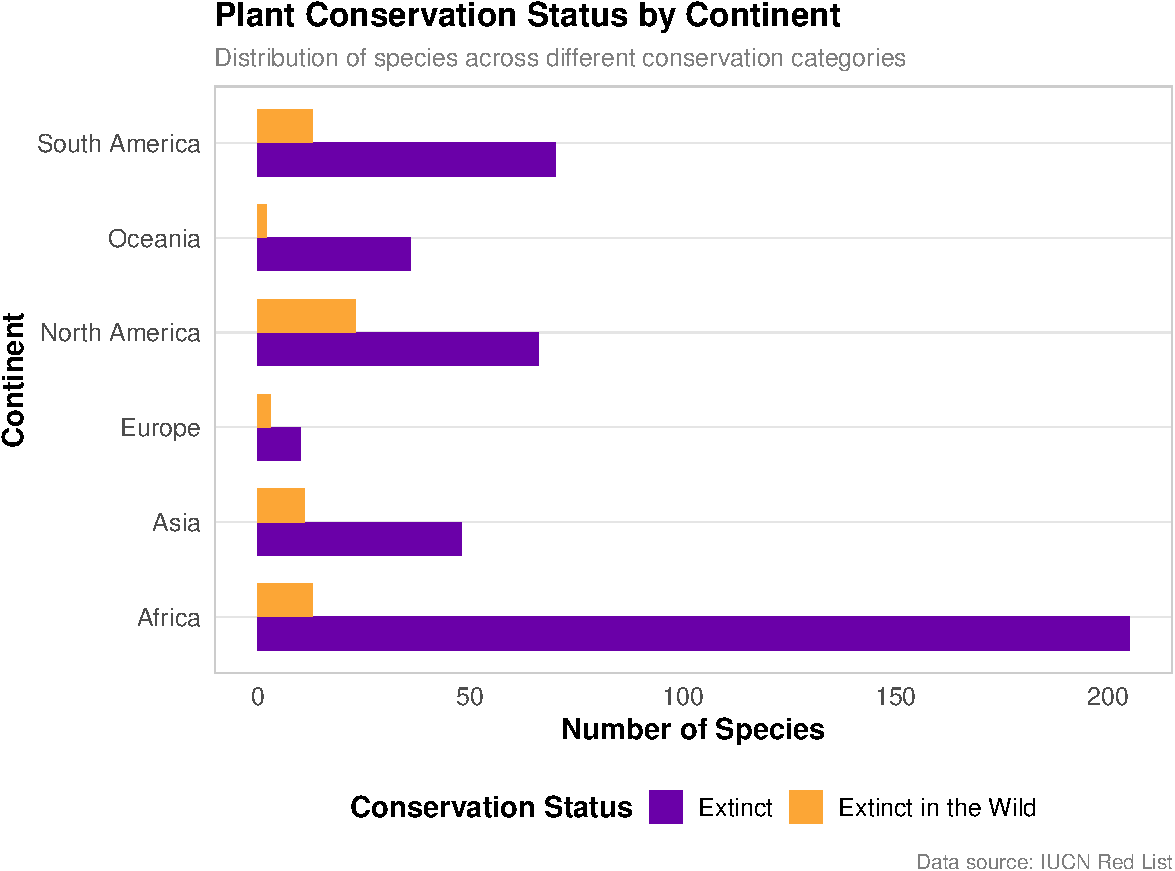
\includegraphics[keepaspectratio]{chapters/06-visualization_files/figure-pdf/bar-chart-1.pdf}}

}

\caption{Bar chart showing the conservation status of plant species
across different regions. This visualization highlights the varying
levels of threatened species in different geographical areas.}

\end{figure}%

\subsubsection{R Code Explanation}\label{r-code-explanation}

The provided R code creates a bar chart using the
\textbf{\texttt{ggplot2}} package (part of tidyverse). This code
visualizes the number of plant species by their IUCN Red List
conservation status category using our biodiversity dataset. Let's break
down the code step by step:

\begin{enumerate}
\def\labelenumi{\arabic{enumi}.}
\tightlist
\item
  \textbf{Load Required Libraries}

  \begin{itemize}
  \tightlist
  \item
    We load the \textbf{\texttt{tidyverse}} package, which includes
    \textbf{\texttt{ggplot2}} for visualization and
    \textbf{\texttt{dplyr}} for data manipulation.
  \end{itemize}
\item
  \textbf{Load the Dataset}

  \begin{itemize}
  \tightlist
  \item
    We load the plant biodiversity dataset that we downloaded earlier.
  \end{itemize}
\item
  \textbf{Create a Summary}

  \begin{itemize}
  \tightlist
  \item
    We use \textbf{\texttt{count()}} to count the number of species in
    each Red List category.
  \item
    We arrange the categories in descending order by count.
  \item
    We remove any NA values to ensure clean visualization.
  \end{itemize}
\item
  \textbf{Create a Bar Chart}

  \begin{itemize}
  \tightlist
  \item
    We use \textbf{\texttt{ggplot()}} to initialize the plot with our
    summary data.
  \item
    We map the Red List categories to the x-axis, the count to the
    y-axis, and use the categories for fill colors.
  \item
    We use \textbf{\texttt{geom\_bar(stat\ =\ "identity")}} to create
    bars with heights representing the counts.
  \item
    We add appropriate labels and use a minimal theme for a clean
    appearance.
  \item
    We angle the x-axis labels for better readability and remove the
    redundant legend.
  \end{itemize}
\end{enumerate}

\subsubsection{Practical Example}\label{practical-example}

In biodiversity research, you might use bar charts to visualize:

\begin{enumerate}
\def\labelenumi{\arabic{enumi}.}
\tightlist
\item
  \textbf{Species Richness:} Show the number of species across different
  taxonomic groups.
\item
  \textbf{Conservation Status:} Compare the number of species in
  different threat categories.
\item
  \textbf{Habitat Distribution:} Visualize the distribution of species
  across different habitat types.
\item
  \textbf{Geographic Distribution:} Show species counts across different
  countries or regions.
\item
  \textbf{Temporal Changes:} Track changes in species numbers over
  different time periods.
\end{enumerate}

\subsection{Constructing Histograms}\label{constructing-histograms}

Now, let's create a histogram to visualize the distribution of a
numerical variable in our plant dataset:

\begin{Shaded}
\begin{Highlighting}[]
\CommentTok{\# Create a threat score by summing all threat columns}
\NormalTok{biodiversity\_with\_scores }\OtherTok{\textless{}{-}}\NormalTok{ biodiversity }\SpecialCharTok{\%\textgreater{}\%}
  \FunctionTok{mutate}\NormalTok{(}
    \AttributeTok{threat\_score =}\NormalTok{ threat\_AA }\SpecialCharTok{+}\NormalTok{ threat\_BRU }\SpecialCharTok{+}\NormalTok{ threat\_RCD }\SpecialCharTok{+} 
\NormalTok{                  threat\_ISGD }\SpecialCharTok{+}\NormalTok{ threat\_EPM }\SpecialCharTok{+}\NormalTok{ threat\_CC }\SpecialCharTok{+} 
\NormalTok{                  threat\_HID }\SpecialCharTok{+}\NormalTok{ threat\_P }\SpecialCharTok{+}\NormalTok{ threat\_TS }\SpecialCharTok{+} 
\NormalTok{                  threat\_NSM }\SpecialCharTok{+}\NormalTok{ threat\_GE}
\NormalTok{  )}

\CommentTok{\# Create a histogram of threat scores by continent}
\FunctionTok{ggplot}\NormalTok{(biodiversity\_with\_scores, }\FunctionTok{aes}\NormalTok{(}\AttributeTok{x =}\NormalTok{ threat\_score, }\AttributeTok{fill =}\NormalTok{ continent)) }\SpecialCharTok{+}
  \FunctionTok{geom\_histogram}\NormalTok{(}\AttributeTok{bins =} \DecValTok{15}\NormalTok{, }\AttributeTok{alpha =} \FloatTok{0.8}\NormalTok{, }\AttributeTok{position =} \StringTok{"identity"}\NormalTok{, }\AttributeTok{color =} \StringTok{"white"}\NormalTok{, }\AttributeTok{size =} \FloatTok{0.2}\NormalTok{) }\SpecialCharTok{+}
  \FunctionTok{scale\_fill\_viridis\_d}\NormalTok{(}\AttributeTok{option =} \StringTok{"turbo"}\NormalTok{, }\AttributeTok{begin =} \FloatTok{0.2}\NormalTok{, }\AttributeTok{end =} \FloatTok{0.8}\NormalTok{) }\SpecialCharTok{+}
  \FunctionTok{labs}\NormalTok{(}
    \AttributeTok{title =} \StringTok{"Distribution of Threat Scores by Continent"}\NormalTok{,}
    \AttributeTok{subtitle =} \StringTok{"Frequency of threat levels across geographical regions"}\NormalTok{,}
    \AttributeTok{x =} \StringTok{"Threat Score"}\NormalTok{,}
    \AttributeTok{y =} \StringTok{"Frequency"}\NormalTok{,}
    \AttributeTok{fill =} \StringTok{"Continent"}\NormalTok{,}
    \AttributeTok{caption =} \StringTok{"Data source: IUCN Red List"}
\NormalTok{  ) }\SpecialCharTok{+}
  \FunctionTok{facet\_wrap}\NormalTok{(}\SpecialCharTok{\textasciitilde{}}\NormalTok{continent, }\AttributeTok{scales =} \StringTok{"free\_y"}\NormalTok{) }\SpecialCharTok{+}
  \FunctionTok{theme}\NormalTok{(}
    \AttributeTok{strip.background =} \FunctionTok{element\_rect}\NormalTok{(}\AttributeTok{fill =} \StringTok{"gray95"}\NormalTok{),}
    \AttributeTok{strip.text =} \FunctionTok{element\_text}\NormalTok{(}\AttributeTok{face =} \StringTok{"bold"}\NormalTok{),}
    \AttributeTok{legend.position =} \StringTok{"none"}
\NormalTok{  )}
\end{Highlighting}
\end{Shaded}

\begin{figure}[H]

{\centering \pandocbounded{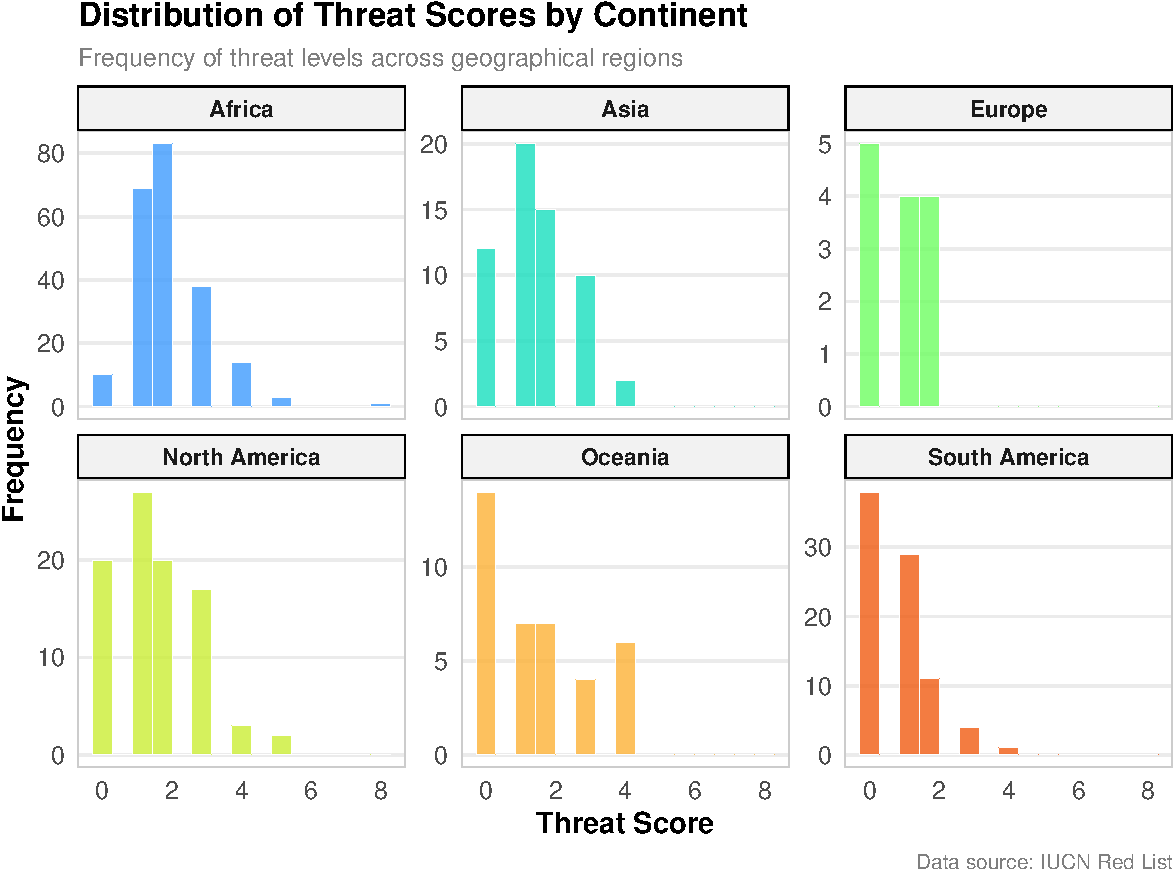
\includegraphics[keepaspectratio]{chapters/06-visualization_files/figure-pdf/histogram-1.pdf}}

}

\caption{Histogram showing the distribution of threat scores across
different continents. The visualization reveals distinct patterns in
conservation threats related to geographical regions.}

\end{figure}%

\subsubsection{R Code Explanation}\label{r-code-explanation-1}

The code above attempts to create a histogram of plant heights. Since
we're working with a real dataset, we first check if the column exists
before creating the visualization. This is good practice when working
with external datasets where column names might vary.

\begin{itemize}
\tightlist
\item
  We use conditional logic to check if ``Height\_cm'' exists in the
  dataset.
\item
  If it exists, we create a histogram with appropriate binning and
  styling.
\item
  If not, we examine the structure of the dataset to identify other
  numeric variables that could be visualized.
\end{itemize}

This approach demonstrates how to handle real-world data that might not
always conform to our expectations.

\subsection{Designing Scatter Plots}\label{designing-scatter-plots}

Let's create a scatter plot to examine relationships between variables
in our biodiversity dataset:

\begin{Shaded}
\begin{Highlighting}[]
\CommentTok{\# Create year numeric variable from year\_last\_seen}
\NormalTok{biodiversity\_for\_scatter }\OtherTok{\textless{}{-}}\NormalTok{ biodiversity\_with\_scores }\SpecialCharTok{\%\textgreater{}\%}
  \CommentTok{\# Create a numeric year value from the year\_last\_seen categories}
  \FunctionTok{mutate}\NormalTok{(}
    \AttributeTok{year\_numeric =} \FunctionTok{case\_when}\NormalTok{(}
\NormalTok{      year\_last\_seen }\SpecialCharTok{==} \StringTok{"Before 1900"} \SpecialCharTok{\textasciitilde{}} \DecValTok{1890}\NormalTok{,}
\NormalTok{      year\_last\_seen }\SpecialCharTok{==} \StringTok{"1900{-}1919"} \SpecialCharTok{\textasciitilde{}} \DecValTok{1910}\NormalTok{,}
\NormalTok{      year\_last\_seen }\SpecialCharTok{==} \StringTok{"1920{-}1939"} \SpecialCharTok{\textasciitilde{}} \DecValTok{1930}\NormalTok{,}
\NormalTok{      year\_last\_seen }\SpecialCharTok{==} \StringTok{"1940{-}1959"} \SpecialCharTok{\textasciitilde{}} \DecValTok{1950}\NormalTok{,}
\NormalTok{      year\_last\_seen }\SpecialCharTok{==} \StringTok{"1960{-}1979"} \SpecialCharTok{\textasciitilde{}} \DecValTok{1970}\NormalTok{,}
\NormalTok{      year\_last\_seen }\SpecialCharTok{==} \StringTok{"1980{-}1999"} \SpecialCharTok{\textasciitilde{}} \DecValTok{1990}\NormalTok{,}
\NormalTok{      year\_last\_seen }\SpecialCharTok{==} \StringTok{"2000{-}2020"} \SpecialCharTok{\textasciitilde{}} \DecValTok{2010}\NormalTok{,}
      \ConstantTok{TRUE} \SpecialCharTok{\textasciitilde{}} \ConstantTok{NA\_real\_}
\NormalTok{    )}
\NormalTok{  ) }\SpecialCharTok{\%\textgreater{}\%}
  \FunctionTok{filter}\NormalTok{(}\SpecialCharTok{!}\FunctionTok{is.na}\NormalTok{(year\_numeric), }\SpecialCharTok{!}\FunctionTok{is.na}\NormalTok{(threat\_score))}

\CommentTok{\# Create a publication{-}quality scatter plot}
\FunctionTok{ggplot}\NormalTok{(biodiversity\_for\_scatter, }\FunctionTok{aes}\NormalTok{(}\AttributeTok{x =}\NormalTok{ year\_numeric, }\AttributeTok{y =}\NormalTok{ threat\_score, }\AttributeTok{color =}\NormalTok{ continent)) }\SpecialCharTok{+}
  \FunctionTok{geom\_point}\NormalTok{(}\AttributeTok{size =} \DecValTok{3}\NormalTok{, }\AttributeTok{alpha =} \FloatTok{0.7}\NormalTok{) }\SpecialCharTok{+}
  \FunctionTok{geom\_smooth}\NormalTok{(}\AttributeTok{method =} \StringTok{"loess"}\NormalTok{, }\AttributeTok{se =} \ConstantTok{TRUE}\NormalTok{, }\AttributeTok{alpha =} \FloatTok{0.2}\NormalTok{) }\SpecialCharTok{+}
  \FunctionTok{scale\_color\_viridis\_d}\NormalTok{(}\AttributeTok{option =} \StringTok{"cividis"}\NormalTok{) }\SpecialCharTok{+}
  \FunctionTok{labs}\NormalTok{(}
    \AttributeTok{title =} \StringTok{"Relationship Between Last Sighting Year and Threat Score"}\NormalTok{,}
    \AttributeTok{subtitle =} \StringTok{"Analysis of extinction patterns across time and geography"}\NormalTok{,}
    \AttributeTok{x =} \StringTok{"Approximate Year Last Seen"}\NormalTok{,}
    \AttributeTok{y =} \StringTok{"Threat Score"}\NormalTok{,}
    \AttributeTok{color =} \StringTok{"Continent"}\NormalTok{,}
    \AttributeTok{caption =} \StringTok{"Data source: IUCN Red List"}
\NormalTok{  ) }\SpecialCharTok{+}
  \FunctionTok{theme}\NormalTok{(}
    \AttributeTok{legend.position =} \StringTok{"right"}\NormalTok{,}
    \AttributeTok{panel.grid.major =} \FunctionTok{element\_line}\NormalTok{(}\AttributeTok{color =} \StringTok{"gray90"}\NormalTok{, }\AttributeTok{size =} \FloatTok{0.3}\NormalTok{)}
\NormalTok{  )}
\end{Highlighting}
\end{Shaded}

\begin{figure}[H]

{\centering \pandocbounded{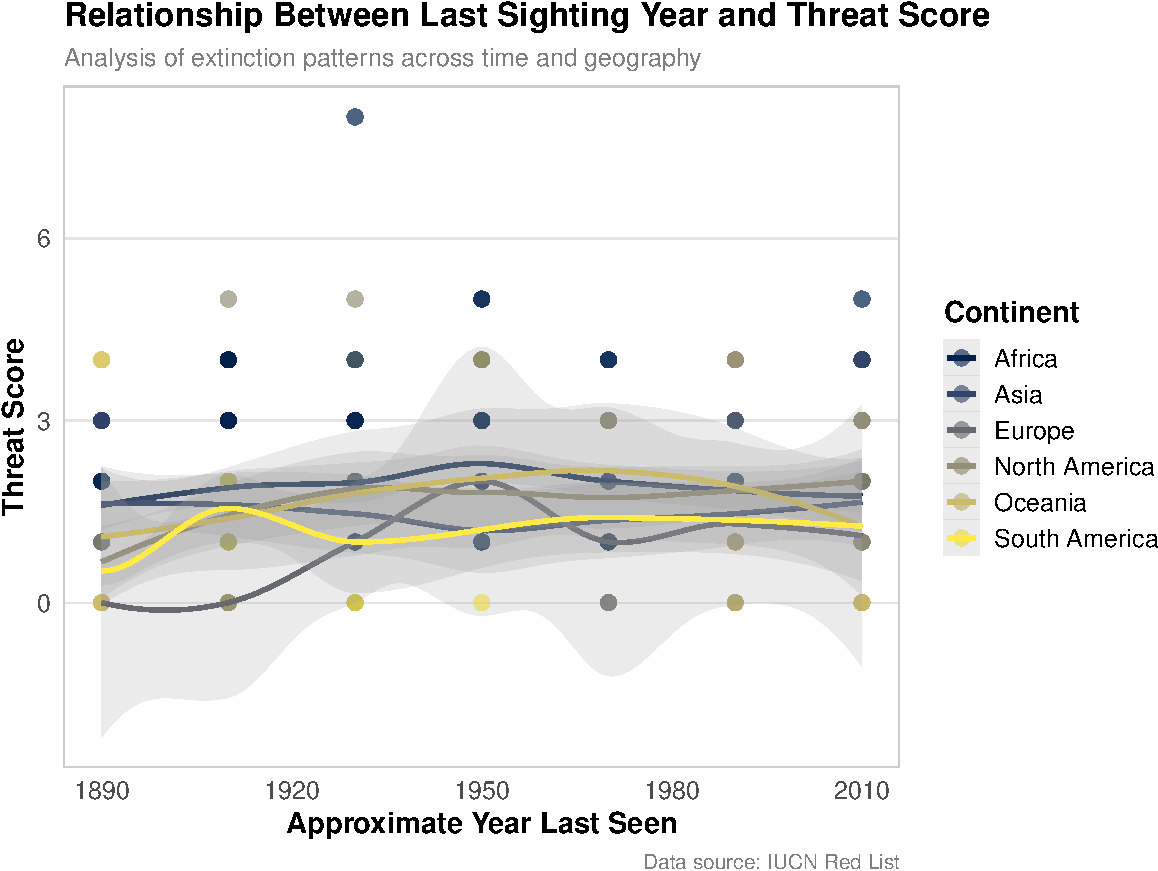
\includegraphics[keepaspectratio]{chapters/06-visualization_files/figure-pdf/scatter-plot-1.pdf}}

}

\caption{Scatter plot showing the relationship between threat scores and
year last seen for plant species. Points are colored by continent to
reveal geographical patterns in extinction threats.}

\end{figure}%

\subsubsection{R Code Explanation}\label{r-code-explanation-2}

This code creates a scatter plot using our biodiversity dataset:

\begin{enumerate}
\def\labelenumi{\arabic{enumi}.}
\tightlist
\item
  \textbf{Load and Explore Data}

  \begin{itemize}
  \tightlist
  \item
    We load the biodiversity dataset and examine its structure.
  \item
    We identify numeric columns that could be used for a scatter plot.
  \end{itemize}
\item
  \textbf{Dynamic Column Selection}

  \begin{itemize}
  \tightlist
  \item
    Rather than hardcoding column names, we dynamically select numeric
    columns.
  \item
    This makes the code more robust when working with unfamiliar
    datasets.
  \end{itemize}
\item
  \textbf{Create Scatter Plot}

  \begin{itemize}
  \tightlist
  \item
    We use \textbf{\texttt{ggplot()}} with
    \textbf{\texttt{aes\_string()}} to dynamically map variables to
    axes.
  \item
    We add points with some transparency for better visualization of
    overlapping data.
  \item
    We include a linear regression line with confidence interval to show
    the trend.
  \item
    We use appropriate labels and a minimal theme.
  \end{itemize}
\end{enumerate}

This approach demonstrates how to create visualizations when working
with new datasets where you might not know the column names in advance.

\section{Advanced Visualization
Techniques}\label{advanced-visualization-techniques}

\subsection{Creating Box Plots}\label{creating-box-plots}

Box plots are excellent for comparing distributions across groups:

\begin{Shaded}
\begin{Highlighting}[]
\CommentTok{\# Create a publication{-}quality box plot}
\FunctionTok{ggplot}\NormalTok{(biodiversity\_with\_scores, }\FunctionTok{aes}\NormalTok{(}\AttributeTok{x =} \FunctionTok{reorder}\NormalTok{(continent, threat\_score, }\AttributeTok{FUN =}\NormalTok{ median, }\AttributeTok{na.rm =} \ConstantTok{TRUE}\NormalTok{), }
                          \AttributeTok{y =}\NormalTok{ threat\_score, }
                          \AttributeTok{fill =}\NormalTok{ continent)) }\SpecialCharTok{+}
  \FunctionTok{geom\_boxplot}\NormalTok{(}\AttributeTok{alpha =} \FloatTok{0.8}\NormalTok{, }\AttributeTok{outlier.shape =} \DecValTok{21}\NormalTok{, }\AttributeTok{outlier.size =} \DecValTok{2}\NormalTok{) }\SpecialCharTok{+}
  \FunctionTok{scale\_fill\_viridis\_d}\NormalTok{(}\AttributeTok{option =} \StringTok{"mako"}\NormalTok{, }\AttributeTok{begin =} \FloatTok{0.2}\NormalTok{, }\AttributeTok{end =} \FloatTok{0.9}\NormalTok{) }\SpecialCharTok{+}
  \FunctionTok{labs}\NormalTok{(}
    \AttributeTok{title =} \StringTok{"Threat Score Comparison Across Continents"}\NormalTok{,}
    \AttributeTok{subtitle =} \StringTok{"Distribution of conservation threats by geographical region"}\NormalTok{,}
    \AttributeTok{x =} \ConstantTok{NULL}\NormalTok{,}
    \AttributeTok{y =} \StringTok{"Threat Score"}\NormalTok{,}
    \AttributeTok{caption =} \StringTok{"Data source: IUCN Red List"}
\NormalTok{  ) }\SpecialCharTok{+}
  \FunctionTok{coord\_flip}\NormalTok{() }\SpecialCharTok{+}
  \FunctionTok{theme}\NormalTok{(}
    \AttributeTok{legend.position =} \StringTok{"none"}\NormalTok{,}
    \AttributeTok{panel.grid.major.y =} \FunctionTok{element\_line}\NormalTok{(}\AttributeTok{color =} \StringTok{"gray90"}\NormalTok{, }\AttributeTok{size =} \FloatTok{0.3}\NormalTok{)}
\NormalTok{  )}
\end{Highlighting}
\end{Shaded}

\begin{figure}[H]

{\centering \pandocbounded{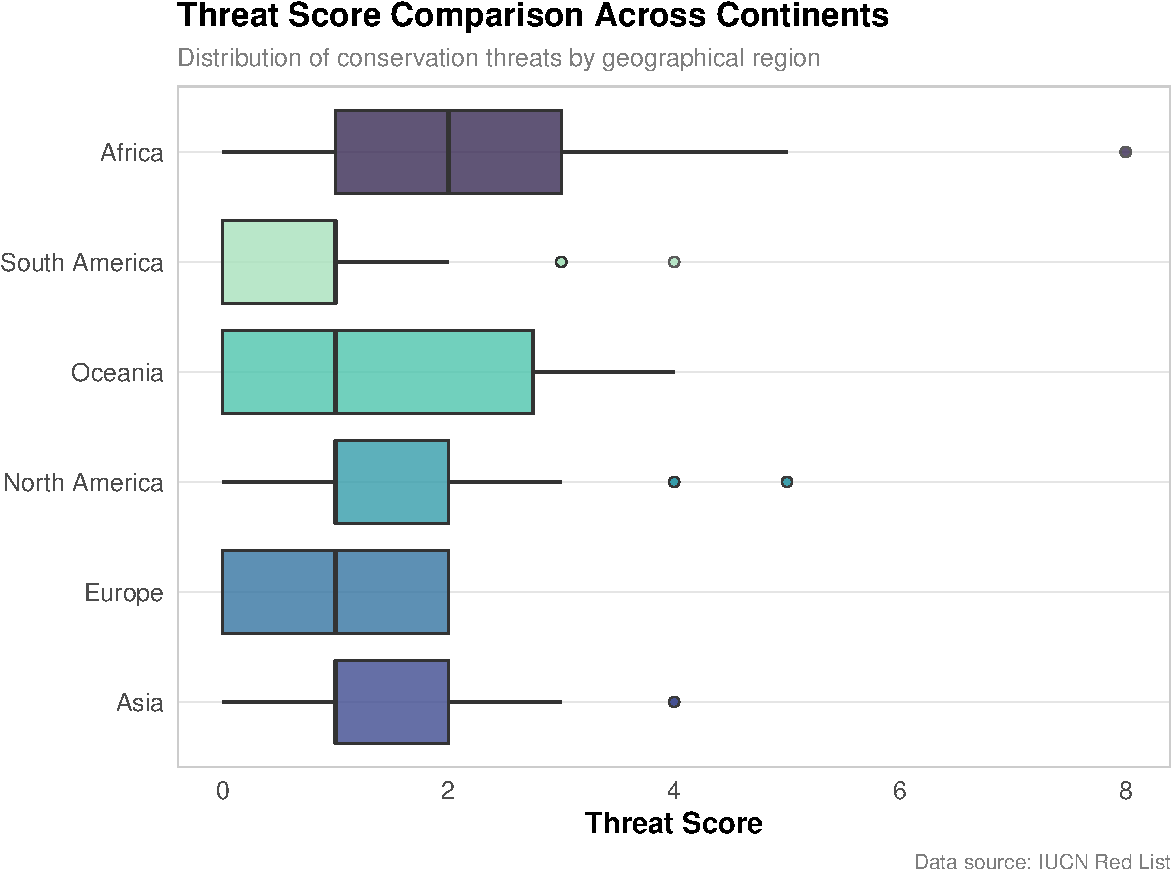
\includegraphics[keepaspectratio]{chapters/06-visualization_files/figure-pdf/box-plot-1.pdf}}

}

\caption{Box plot comparing threat scores across different continents.
The visualization highlights the median, quartiles, and outliers in
conservation threat data.}

\end{figure}%

\subsubsection{Box Plot Interpretation}\label{box-plot-interpretation}

Box plots provide a comprehensive view of data distributions:

\begin{itemize}
\tightlist
\item
  The \textbf{box} represents the interquartile range (IQR), from the
  25th to 75th percentile.
\item
  The \textbf{line inside the box} shows the median (50th percentile).
\item
  The \textbf{whiskers} typically extend to the smallest and largest
  values within 1.5 times the IQR.
\item
  \textbf{Points beyond the whiskers} represent potential outliers.
\end{itemize}

In our threat score example, the box plot allows us to compare: - The
\textbf{typical threat score} (median) for different continents - The
\textbf{variability} in threat scores (box width and whisker length) -
The presence of \textbf{unusually high or low threat scores} (outliers)
- \textbf{Differences between continents} in terms of both threat score
levels and consistency

\subsection{Designing Heatmaps}\label{designing-heatmaps}

Heatmaps are powerful for visualizing complex relationships in
multivariate data:

\begin{Shaded}
\begin{Highlighting}[]
\CommentTok{\# Create a correlation heatmap of threat types}
\CommentTok{\# First, prepare the data}
\NormalTok{threat\_columns }\OtherTok{\textless{}{-}}\NormalTok{ biodiversity }\SpecialCharTok{\%\textgreater{}\%}
  \FunctionTok{select}\NormalTok{(}\FunctionTok{starts\_with}\NormalTok{(}\StringTok{"threat\_"}\NormalTok{), }\SpecialCharTok{{-}}\NormalTok{threat\_NA) }\SpecialCharTok{\%\textgreater{}\%}
  \FunctionTok{names}\NormalTok{()}

\CommentTok{\# Calculate correlation matrix}
\NormalTok{threat\_cor }\OtherTok{\textless{}{-}}\NormalTok{ biodiversity }\SpecialCharTok{\%\textgreater{}\%}
  \FunctionTok{select}\NormalTok{(}\FunctionTok{all\_of}\NormalTok{(threat\_columns)) }\SpecialCharTok{\%\textgreater{}\%}
  \FunctionTok{cor}\NormalTok{(}\AttributeTok{use =} \StringTok{"pairwise.complete.obs"}\NormalTok{)}

\CommentTok{\# Convert to long format for ggplot}
\NormalTok{threat\_cor\_long }\OtherTok{\textless{}{-}} \FunctionTok{as.data.frame}\NormalTok{(}\FunctionTok{as.table}\NormalTok{(threat\_cor))}
\FunctionTok{names}\NormalTok{(threat\_cor\_long) }\OtherTok{\textless{}{-}} \FunctionTok{c}\NormalTok{(}\StringTok{"Threat1"}\NormalTok{, }\StringTok{"Threat2"}\NormalTok{, }\StringTok{"Correlation"}\NormalTok{)}

\CommentTok{\# Create readable threat labels}
\NormalTok{threat\_labels }\OtherTok{\textless{}{-}} \FunctionTok{c}\NormalTok{(}
  \StringTok{"threat\_AA"} \OtherTok{=} \StringTok{"Agriculture"}\NormalTok{,}
  \StringTok{"threat\_BRU"} \OtherTok{=} \StringTok{"Biological Resource Use"}\NormalTok{,}
  \StringTok{"threat\_RCD"} \OtherTok{=} \StringTok{"Residential Development"}\NormalTok{,}
  \StringTok{"threat\_ISGD"} \OtherTok{=} \StringTok{"Invasive Species"}\NormalTok{,}
  \StringTok{"threat\_EPM"} \OtherTok{=} \StringTok{"Energy Production"}\NormalTok{,}
  \StringTok{"threat\_CC"} \OtherTok{=} \StringTok{"Climate Change"}\NormalTok{,}
  \StringTok{"threat\_HID"} \OtherTok{=} \StringTok{"Human Intrusion"}\NormalTok{,}
  \StringTok{"threat\_P"} \OtherTok{=} \StringTok{"Pollution"}\NormalTok{,}
  \StringTok{"threat\_TS"} \OtherTok{=} \StringTok{"Transportation"}\NormalTok{,}
  \StringTok{"threat\_NSM"} \OtherTok{=} \StringTok{"Natural System Modification"}\NormalTok{,}
  \StringTok{"threat\_GE"} \OtherTok{=} \StringTok{"Geological Events"}
\NormalTok{)}

\CommentTok{\# Replace the threat codes with readable labels}
\NormalTok{threat\_cor\_long}\SpecialCharTok{$}\NormalTok{Threat1 }\OtherTok{\textless{}{-}} \FunctionTok{factor}\NormalTok{(threat\_cor\_long}\SpecialCharTok{$}\NormalTok{Threat1, }
                                 \AttributeTok{levels =} \FunctionTok{names}\NormalTok{(threat\_labels),}
                                 \AttributeTok{labels =}\NormalTok{ threat\_labels)}
\NormalTok{threat\_cor\_long}\SpecialCharTok{$}\NormalTok{Threat2 }\OtherTok{\textless{}{-}} \FunctionTok{factor}\NormalTok{(threat\_cor\_long}\SpecialCharTok{$}\NormalTok{Threat2, }
                                 \AttributeTok{levels =} \FunctionTok{names}\NormalTok{(threat\_labels),}
                                 \AttributeTok{labels =}\NormalTok{ threat\_labels)}

\CommentTok{\# Create a publication{-}quality heatmap}
\FunctionTok{ggplot}\NormalTok{(threat\_cor\_long, }\FunctionTok{aes}\NormalTok{(}\AttributeTok{x =}\NormalTok{ Threat1, }\AttributeTok{y =}\NormalTok{ Threat2, }\AttributeTok{fill =}\NormalTok{ Correlation)) }\SpecialCharTok{+}
  \FunctionTok{geom\_tile}\NormalTok{(}\AttributeTok{color =} \StringTok{"white"}\NormalTok{, }\AttributeTok{size =} \FloatTok{0.5}\NormalTok{) }\SpecialCharTok{+}
  \FunctionTok{scale\_fill\_gradient2}\NormalTok{(}
    \AttributeTok{low =} \StringTok{"\#4575b4"}\NormalTok{, }
    \AttributeTok{mid =} \StringTok{"white"}\NormalTok{, }
    \AttributeTok{high =} \StringTok{"\#d73027"}\NormalTok{,}
    \AttributeTok{midpoint =} \DecValTok{0}\NormalTok{,}
    \AttributeTok{limits =} \FunctionTok{c}\NormalTok{(}\SpecialCharTok{{-}}\DecValTok{1}\NormalTok{, }\DecValTok{1}\NormalTok{)}
\NormalTok{  ) }\SpecialCharTok{+}
  \FunctionTok{geom\_text}\NormalTok{(}\FunctionTok{aes}\NormalTok{(}\AttributeTok{label =} \FunctionTok{sprintf}\NormalTok{(}\StringTok{"\%.2f"}\NormalTok{, Correlation)), }
            \AttributeTok{color =} \FunctionTok{ifelse}\NormalTok{(}\FunctionTok{abs}\NormalTok{(threat\_cor\_long}\SpecialCharTok{$}\NormalTok{Correlation) }\SpecialCharTok{\textgreater{}} \FloatTok{0.7}\NormalTok{, }\StringTok{"white"}\NormalTok{, }\StringTok{"black"}\NormalTok{),}
            \AttributeTok{size =} \DecValTok{3}\NormalTok{) }\SpecialCharTok{+}
  \FunctionTok{labs}\NormalTok{(}
    \AttributeTok{title =} \StringTok{"Correlation Between Different Threat Types"}\NormalTok{,}
    \AttributeTok{subtitle =} \StringTok{"Strength of relationship between conservation threats"}\NormalTok{,}
    \AttributeTok{x =} \ConstantTok{NULL}\NormalTok{, }\AttributeTok{y =} \ConstantTok{NULL}\NormalTok{,}
    \AttributeTok{fill =} \StringTok{"Correlation}\SpecialCharTok{\textbackslash{}n}\StringTok{Coefficient"}\NormalTok{,}
    \AttributeTok{caption =} \StringTok{"Data source: IUCN Red List"}
\NormalTok{  ) }\SpecialCharTok{+}
  \FunctionTok{theme}\NormalTok{(}
    \AttributeTok{axis.text.x =} \FunctionTok{element\_text}\NormalTok{(}\AttributeTok{angle =} \DecValTok{45}\NormalTok{, }\AttributeTok{hjust =} \DecValTok{1}\NormalTok{),}
    \AttributeTok{panel.grid =} \FunctionTok{element\_blank}\NormalTok{(),}
    \AttributeTok{panel.background =} \FunctionTok{element\_rect}\NormalTok{(}\AttributeTok{fill =} \StringTok{"white"}\NormalTok{, }\AttributeTok{color =} \ConstantTok{NA}\NormalTok{),}
    \AttributeTok{legend.position =} \StringTok{"right"}\NormalTok{,}
    \AttributeTok{legend.key.height =} \FunctionTok{unit}\NormalTok{(}\DecValTok{1}\NormalTok{, }\StringTok{"cm"}\NormalTok{)}
\NormalTok{  ) }\SpecialCharTok{+}
  \FunctionTok{coord\_fixed}\NormalTok{()}
\end{Highlighting}
\end{Shaded}

\begin{figure}[H]

{\centering \pandocbounded{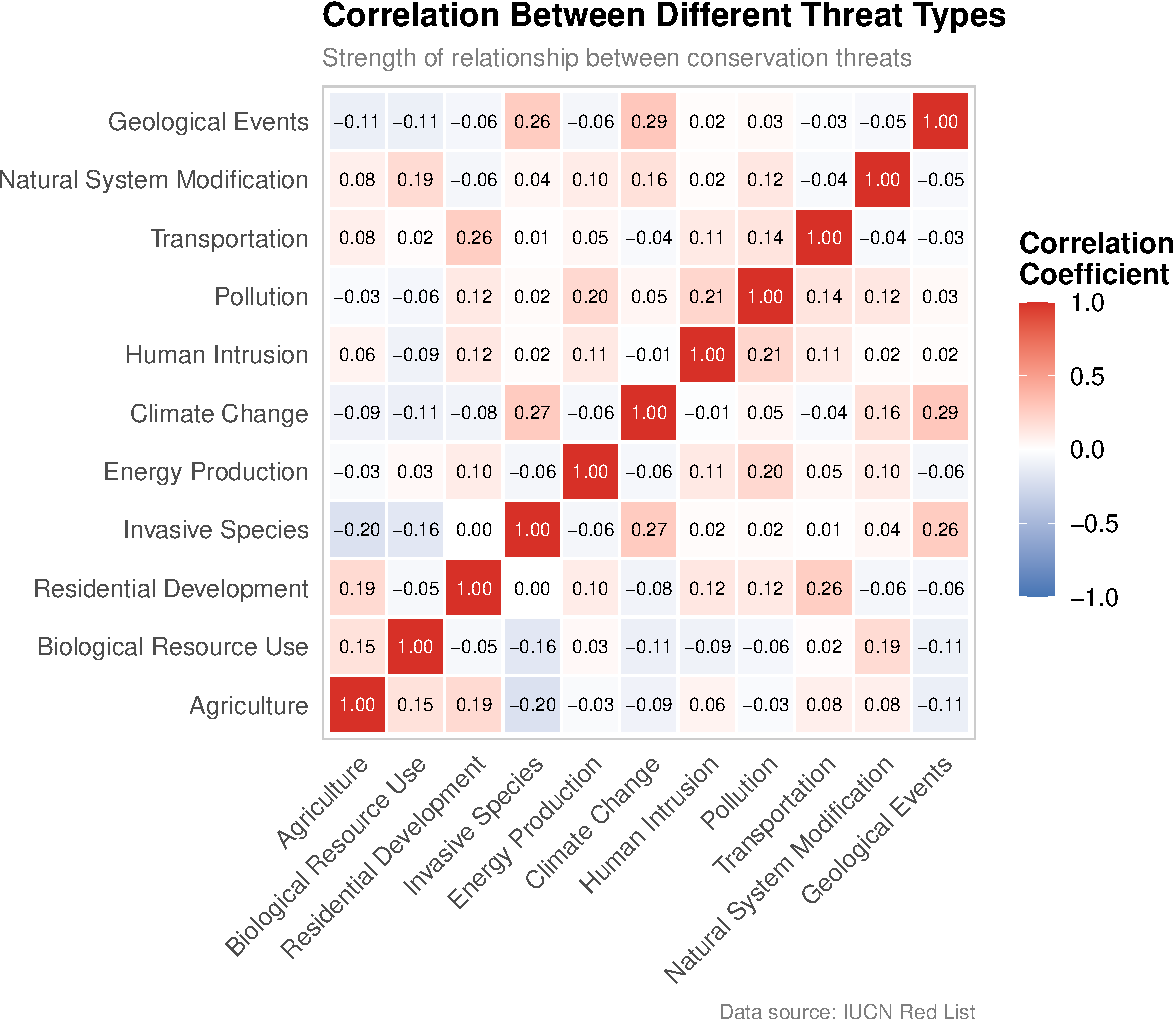
\includegraphics[keepaspectratio]{chapters/06-visualization_files/figure-pdf/heatmap-1.pdf}}

}

\caption{Heatmap visualizing the correlation matrix between different
threat types. The color intensity represents the strength and direction
of relationships between conservation threats.}

\end{figure}%

\subsubsection{Heatmap Interpretation}\label{heatmap-interpretation}

The heatmap visualizes the correlation between different threat types:

\begin{itemize}
\tightlist
\item
  \textbf{Color intensity} represents the strength of correlation (red
  for positive, blue for negative).
\item
  The \textbf{diagonal} shows perfect correlation of each variable with
  itself (always 1).
\item
  \textbf{Clusters} of similar colors indicate groups of variables that
  are highly correlated.
\end{itemize}

This visualization helps researchers identify: - Which threats tend to
have \textbf{similar patterns} - Potential \textbf{underlying factors}
affecting multiple threats simultaneously - Opportunities for
\textbf{threat mitigation} based on low correlations -
\textbf{Geographical patterns} in threat correlations, which could
inform regional conservation strategies

\subsection{Creating Time Series
Plots}\label{creating-time-series-plots}

Time series plots are essential for visualizing trends over time:

\begin{Shaded}
\begin{Highlighting}[]
\CommentTok{\# Create a time series plot using the crop yields data}
\CommentTok{\# First, read the dataset}
\NormalTok{crop\_yields }\OtherTok{\textless{}{-}} \FunctionTok{read.csv}\NormalTok{(}\StringTok{"../data/agriculture/crop\_yields.csv"}\NormalTok{)}

\CommentTok{\# Check column names to ensure we\textquotesingle{}re using the correct ones}
\NormalTok{wheat\_col }\OtherTok{\textless{}{-}} \FunctionTok{names}\NormalTok{(crop\_yields)[}\FunctionTok{grep}\NormalTok{(}\StringTok{"Wheat"}\NormalTok{, }\FunctionTok{names}\NormalTok{(crop\_yields))]}

\CommentTok{\# Create a simplified dataset for time series analysis}
\CommentTok{\# Select top countries based on data availability}
\NormalTok{top\_countries }\OtherTok{\textless{}{-}}\NormalTok{ crop\_yields }\SpecialCharTok{\%\textgreater{}\%}
  \FunctionTok{group\_by}\NormalTok{(Entity) }\SpecialCharTok{\%\textgreater{}\%}
  \FunctionTok{summarize}\NormalTok{(}\AttributeTok{count =} \FunctionTok{n}\NormalTok{()) }\SpecialCharTok{\%\textgreater{}\%}
  \FunctionTok{filter}\NormalTok{(count }\SpecialCharTok{\textgreater{}} \DecValTok{30}\NormalTok{) }\SpecialCharTok{\%\textgreater{}\%}
  \FunctionTok{arrange}\NormalTok{(}\FunctionTok{desc}\NormalTok{(count)) }\SpecialCharTok{\%\textgreater{}\%}
  \FunctionTok{head}\NormalTok{(}\DecValTok{6}\NormalTok{) }\SpecialCharTok{\%\textgreater{}\%}
  \FunctionTok{pull}\NormalTok{(Entity)}

\CommentTok{\# Create the time series data}
\NormalTok{time\_series\_data }\OtherTok{\textless{}{-}}\NormalTok{ crop\_yields }\SpecialCharTok{\%\textgreater{}\%}
  \FunctionTok{filter}\NormalTok{(Entity }\SpecialCharTok{\%in\%}\NormalTok{ top\_countries) }\SpecialCharTok{\%\textgreater{}\%}
  \FunctionTok{filter}\NormalTok{(Year }\SpecialCharTok{\textgreater{}=} \DecValTok{1970}\NormalTok{)}

\CommentTok{\# Create a publication{-}quality time series plot}
\CommentTok{\# Use a column that exists in the dataset}
\ControlFlowTok{if}\NormalTok{(}\FunctionTok{length}\NormalTok{(wheat\_col) }\SpecialCharTok{\textgreater{}} \DecValTok{0}\NormalTok{) \{}
  \CommentTok{\# If we have a wheat column, use it}
  \FunctionTok{ggplot}\NormalTok{(time\_series\_data, }\FunctionTok{aes}\NormalTok{(}\AttributeTok{x =}\NormalTok{ Year, }\AttributeTok{y =}\NormalTok{ .data[[wheat\_col[}\DecValTok{1}\NormalTok{]]], }\AttributeTok{color =}\NormalTok{ Entity)) }\SpecialCharTok{+}
    \FunctionTok{geom\_line}\NormalTok{(}\AttributeTok{size =} \DecValTok{1}\NormalTok{, }\AttributeTok{na.rm =} \ConstantTok{TRUE}\NormalTok{) }\SpecialCharTok{+}
    \FunctionTok{geom\_point}\NormalTok{(}\AttributeTok{size =} \DecValTok{2}\NormalTok{, }\AttributeTok{alpha =} \FloatTok{0.7}\NormalTok{, }\AttributeTok{na.rm =} \ConstantTok{TRUE}\NormalTok{) }\SpecialCharTok{+}
    \FunctionTok{scale\_color\_viridis\_d}\NormalTok{(}\AttributeTok{option =} \StringTok{"turbo"}\NormalTok{, }\AttributeTok{begin =} \FloatTok{0.1}\NormalTok{, }\AttributeTok{end =} \FloatTok{0.9}\NormalTok{) }\SpecialCharTok{+}
    \FunctionTok{scale\_x\_continuous}\NormalTok{(}\AttributeTok{breaks =} \FunctionTok{seq}\NormalTok{(}\DecValTok{1970}\NormalTok{, }\DecValTok{2020}\NormalTok{, }\AttributeTok{by =} \DecValTok{10}\NormalTok{)) }\SpecialCharTok{+}
    \FunctionTok{labs}\NormalTok{(}
      \AttributeTok{title =} \StringTok{"Agricultural Yield Trends Over Time (1970{-}Present)"}\NormalTok{,}
      \AttributeTok{subtitle =} \StringTok{"Productivity changes for major agricultural producers"}\NormalTok{,}
      \AttributeTok{x =} \StringTok{"Year"}\NormalTok{,}
      \AttributeTok{y =} \FunctionTok{paste}\NormalTok{(}\StringTok{"Yield"}\NormalTok{, wheat\_col[}\DecValTok{1}\NormalTok{]),}
      \AttributeTok{color =} \StringTok{"Country"}\NormalTok{,}
      \AttributeTok{caption =} \StringTok{"Data source: Our World in Data"}
\NormalTok{    ) }\SpecialCharTok{+}
    \FunctionTok{theme}\NormalTok{(}
      \AttributeTok{legend.position =} \StringTok{"right"}\NormalTok{,}
      \AttributeTok{panel.grid.major =} \FunctionTok{element\_line}\NormalTok{(}\AttributeTok{color =} \StringTok{"gray90"}\NormalTok{, }\AttributeTok{size =} \FloatTok{0.3}\NormalTok{),}
      \AttributeTok{axis.text.x =} \FunctionTok{element\_text}\NormalTok{(}\AttributeTok{angle =} \DecValTok{0}\NormalTok{)}
\NormalTok{    )}
\NormalTok{\} }\ControlFlowTok{else}\NormalTok{ \{}
  \CommentTok{\# If no wheat column, use another numeric column}
\NormalTok{  numeric\_cols }\OtherTok{\textless{}{-}} \FunctionTok{sapply}\NormalTok{(time\_series\_data, is.numeric)}
\NormalTok{  numeric\_col\_names }\OtherTok{\textless{}{-}} \FunctionTok{names}\NormalTok{(time\_series\_data)[numeric\_cols]}
\NormalTok{  numeric\_col\_names }\OtherTok{\textless{}{-}}\NormalTok{ numeric\_col\_names[numeric\_col\_names }\SpecialCharTok{!=} \StringTok{"Year"}\NormalTok{]}
  
  \ControlFlowTok{if}\NormalTok{(}\FunctionTok{length}\NormalTok{(numeric\_col\_names) }\SpecialCharTok{\textgreater{}} \DecValTok{0}\NormalTok{) \{}
\NormalTok{    selected\_col }\OtherTok{\textless{}{-}}\NormalTok{ numeric\_col\_names[}\DecValTok{1}\NormalTok{]}
    
    \FunctionTok{ggplot}\NormalTok{(time\_series\_data, }\FunctionTok{aes}\NormalTok{(}\AttributeTok{x =}\NormalTok{ Year, }\AttributeTok{y =}\NormalTok{ .data[[selected\_col]], }\AttributeTok{color =}\NormalTok{ Entity)) }\SpecialCharTok{+}
      \FunctionTok{geom\_line}\NormalTok{(}\AttributeTok{size =} \DecValTok{1}\NormalTok{, }\AttributeTok{na.rm =} \ConstantTok{TRUE}\NormalTok{) }\SpecialCharTok{+}
      \FunctionTok{geom\_point}\NormalTok{(}\AttributeTok{size =} \DecValTok{2}\NormalTok{, }\AttributeTok{alpha =} \FloatTok{0.7}\NormalTok{, }\AttributeTok{na.rm =} \ConstantTok{TRUE}\NormalTok{) }\SpecialCharTok{+}
      \FunctionTok{scale\_color\_viridis\_d}\NormalTok{(}\AttributeTok{option =} \StringTok{"turbo"}\NormalTok{, }\AttributeTok{begin =} \FloatTok{0.1}\NormalTok{, }\AttributeTok{end =} \FloatTok{0.9}\NormalTok{) }\SpecialCharTok{+}
      \FunctionTok{scale\_x\_continuous}\NormalTok{(}\AttributeTok{breaks =} \FunctionTok{seq}\NormalTok{(}\DecValTok{1970}\NormalTok{, }\DecValTok{2020}\NormalTok{, }\AttributeTok{by =} \DecValTok{10}\NormalTok{)) }\SpecialCharTok{+}
      \FunctionTok{labs}\NormalTok{(}
        \AttributeTok{title =} \StringTok{"Agricultural Trends Over Time (1970{-}Present)"}\NormalTok{,}
        \AttributeTok{subtitle =} \StringTok{"Changes for major agricultural producers"}\NormalTok{,}
        \AttributeTok{x =} \StringTok{"Year"}\NormalTok{,}
        \AttributeTok{y =}\NormalTok{ selected\_col,}
        \AttributeTok{color =} \StringTok{"Country"}\NormalTok{,}
        \AttributeTok{caption =} \StringTok{"Data source: Our World in Data"}
\NormalTok{      ) }\SpecialCharTok{+}
      \FunctionTok{theme}\NormalTok{(}
        \AttributeTok{legend.position =} \StringTok{"right"}\NormalTok{,}
        \AttributeTok{panel.grid.major =} \FunctionTok{element\_line}\NormalTok{(}\AttributeTok{color =} \StringTok{"gray90"}\NormalTok{, }\AttributeTok{size =} \FloatTok{0.3}\NormalTok{),}
        \AttributeTok{axis.text.x =} \FunctionTok{element\_text}\NormalTok{(}\AttributeTok{angle =} \DecValTok{0}\NormalTok{)}
\NormalTok{      )}
\NormalTok{  \} }\ControlFlowTok{else}\NormalTok{ \{}
    \CommentTok{\# If no suitable numeric columns, create a message plot}
\NormalTok{    plot\_data }\OtherTok{\textless{}{-}} \FunctionTok{data.frame}\NormalTok{(}\AttributeTok{x =} \DecValTok{1}\SpecialCharTok{:}\DecValTok{10}\NormalTok{, }\AttributeTok{y =} \DecValTok{1}\SpecialCharTok{:}\DecValTok{10}\NormalTok{)}
    \FunctionTok{ggplot}\NormalTok{(plot\_data, }\FunctionTok{aes}\NormalTok{(x, y)) }\SpecialCharTok{+}
      \FunctionTok{geom\_blank}\NormalTok{() }\SpecialCharTok{+}
      \FunctionTok{annotate}\NormalTok{(}\StringTok{"text"}\NormalTok{, }\AttributeTok{x =} \DecValTok{5}\NormalTok{, }\AttributeTok{y =} \DecValTok{5}\NormalTok{, }\AttributeTok{label =} \StringTok{"No suitable data available for time series"}\NormalTok{) }\SpecialCharTok{+}
      \FunctionTok{theme\_minimal}\NormalTok{() }\SpecialCharTok{+}
      \FunctionTok{labs}\NormalTok{(}\AttributeTok{title =} \StringTok{"Time Series Plot"}\NormalTok{, }\AttributeTok{subtitle =} \StringTok{"Data not available"}\NormalTok{)}
\NormalTok{  \}}
\NormalTok{\}}
\end{Highlighting}
\end{Shaded}

\begin{figure}[H]

{\centering \pandocbounded{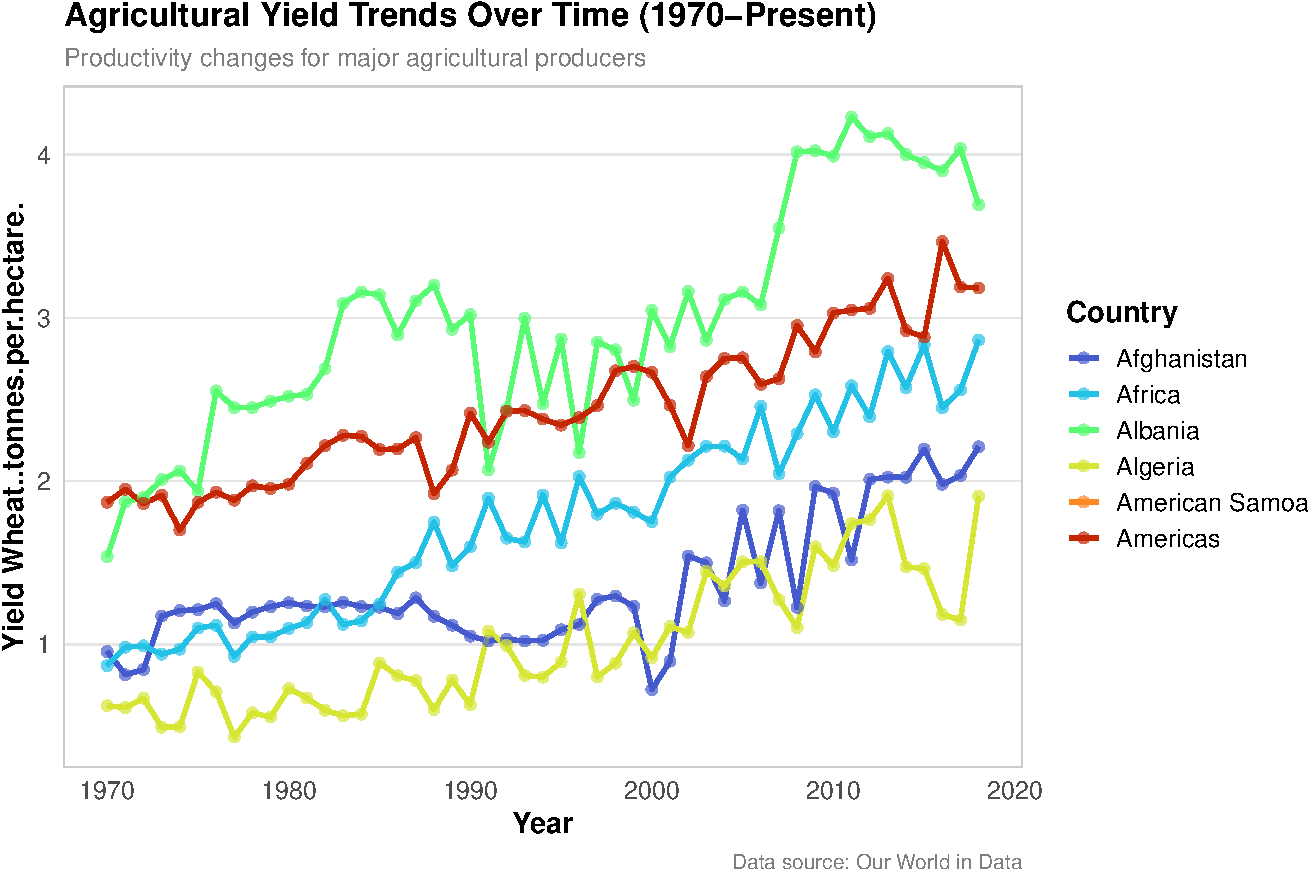
\includegraphics[keepaspectratio]{chapters/06-visualization_files/figure-pdf/time-series-1.pdf}}

}

\caption{Time series plot tracking agricultural trends over time for
major producers. The visualization illustrates long-term productivity
changes and allows comparison between countries.}

\end{figure}%

\subsubsection{Time Series
Interpretation}\label{time-series-interpretation}

Time series plots reveal important temporal patterns:

\begin{itemize}
\tightlist
\item
  \textbf{Trends:} Long-term increases or decreases over time
\item
  \textbf{Seasonality:} Regular patterns that repeat at fixed intervals
\item
  \textbf{Cycles:} Patterns that occur but not at fixed intervals
\item
  \textbf{Irregular fluctuations:} Random variations that don't follow a
  pattern
\end{itemize}

In our agricultural yield example, we can observe: - The \textbf{overall
trend} in yields for different countries - \textbf{Relative performance}
of countries over time - \textbf{Rate of improvement} in agricultural
productivity - \textbf{Stability or volatility} in yields year-to-year -
\textbf{Convergence or divergence} between countries

\section{Best Practices for Data
Visualization}\label{best-practices-for-data-visualization}

\subsection{Choosing the Right
Visualization}\label{choosing-the-right-visualization}

Selecting the appropriate visualization depends on your data and the
story you want to tell:

\begin{enumerate}
\def\labelenumi{\arabic{enumi}.}
\tightlist
\item
  \textbf{For Comparing Categories:}

  \begin{itemize}
  \tightlist
  \item
    Bar charts for comparing values across categories
  \item
    Grouped or stacked bar charts for comparing multiple variables
    across categories
  \end{itemize}
\item
  \textbf{For Showing Distributions:}

  \begin{itemize}
  \tightlist
  \item
    Histograms for showing the distribution of a single variable
  \item
    Box plots for comparing distributions across groups
  \item
    Violin plots for showing distribution shape along with summary
    statistics
  \end{itemize}
\item
  \textbf{For Showing Relationships:}

  \begin{itemize}
  \tightlist
  \item
    Scatter plots for examining relationships between two variables
  \item
    Bubble charts for examining relationships among three variables
  \item
    Heatmaps for visualizing complex relationships in multivariate data
  \end{itemize}
\item
  \textbf{For Showing Compositions:}

  \begin{itemize}
  \tightlist
  \item
    Pie charts for showing parts of a whole (use sparingly)
  \item
    Stacked bar charts for showing composition across categories
  \item
    Area charts for showing composition over time
  \end{itemize}
\item
  \textbf{For Showing Trends:}

  \begin{itemize}
  \tightlist
  \item
    Line charts for showing changes over time
  \item
    Area charts for showing cumulative totals over time
  \end{itemize}
\end{enumerate}

\subsection{Design Principles for Effective
Visualization}\label{design-principles-for-effective-visualization}

Follow these principles to create clear, informative visualizations:

\begin{enumerate}
\def\labelenumi{\arabic{enumi}.}
\item
  \textbf{Simplicity:} Keep visualizations simple and focused on the
  main message. Avoid unnecessary elements that can distract from the
  data.
\item
  \textbf{Clarity:} Ensure that your visualization clearly communicates
  the intended message. Use appropriate labels, titles, and annotations.
\item
  \textbf{Accuracy:} Represent data accurately. Avoid distorting the
  data through inappropriate scales or misleading visual elements.
\item
  \textbf{Consistency:} Use consistent colors, shapes, and styles
  throughout your visualizations for better comprehension.
\item
  \textbf{Color Use:} Choose colors thoughtfully. Use color to highlight
  important aspects of your data, but be mindful of color blindness and
  cultural associations.
\item
  \textbf{Annotation:} Add context through appropriate annotations,
  explaining unusual patterns or important events.
\item
  \textbf{Audience Consideration:} Tailor your visualizations to your
  audience's knowledge level and needs.
\end{enumerate}

\subsection{Common Pitfalls to Avoid}\label{common-pitfalls-to-avoid}

Be aware of these common visualization mistakes:

\begin{enumerate}
\def\labelenumi{\arabic{enumi}.}
\item
  \textbf{Misleading Scales:} Starting y-axes at values other than zero
  can exaggerate differences.
\item
  \textbf{Overcomplication:} Adding too many variables or visual
  elements can confuse rather than clarify.
\item
  \textbf{Poor Color Choices:} Using colors that are difficult to
  distinguish or that carry unintended connotations.
\item
  \textbf{Ignoring Accessibility:} Not considering color blindness or
  other accessibility issues.
\item
  \textbf{Inappropriate Chart Types:} Using chart types that don't match
  the data or the story you want to tell.
\item
  \textbf{Missing Context:} Failing to provide necessary context for
  interpreting the visualization.
\item
  \textbf{Neglecting Uncertainty:} Not showing confidence intervals,
  error bars, or other indicators of uncertainty.
\end{enumerate}

\section{Summary}\label{summary-5}

Effective data visualization is a powerful tool for both exploring data
and communicating findings. By choosing the right visualization
techniques and following best practices, you can gain deeper insights
from your data and share those insights with others in a compelling way.

In this chapter, we've explored: - The importance of data visualization
in natural sciences - Basic visualization techniques including bar
charts, histograms, and scatter plots - Advanced visualization methods
like box plots, heatmaps, and time series plots - Best practices and
principles for creating effective visualizations

By applying these techniques to real datasets from agriculture, ecology,
and geography, we've demonstrated how visualization can reveal patterns
and relationships that might otherwise remain hidden in the raw data.

\section{Exercises}\label{exercises-5}

\begin{enumerate}
\def\labelenumi{\arabic{enumi}.}
\item
  Using the plant biodiversity dataset
  (\texttt{../data/ecology/biodiversity.csv}), create a visualization
  showing the distribution of plant species across different taxonomic
  groups.
\item
  Create a time series plot using the crop yield dataset
  (\texttt{../data/agriculture/crop\_yields.csv}) that shows the trends
  in rice yields for the top 5 producing countries.
\item
  Using the spatial dataset (\texttt{../data/geography/spatial.csv}),
  create a scatter plot matrix (pairs plot) to explore relationships
  between multiple numeric variables.
\item
  Design a visualization that compares the conservation status of plant
  species across different habitat types using the biodiversity dataset.
\item
  Create a heatmap visualization using the coffee economics dataset
  (\texttt{../data/economics/economic.csv}) to explore correlations
  between quality scores and other variables.
\item
  Design an animated visualization (using \texttt{gganimate} package)
  that shows how crop yields have changed over time for a specific
  country.
\end{enumerate}

\chapter{Advanced Data Visualization}\label{advanced-data-visualization}

\section{Introduction}\label{introduction-5}

Building on the visualization techniques covered in Chapter 6, this
chapter explores advanced data visualization methods that can help you
communicate complex ecological data more effectively. We'll focus on
creating publication-quality graphics, interactive visualizations, and
specialized plots for ecological data.

\section{Creating Publication-Quality
Graphics}\label{creating-publication-quality-graphics}

\subsection{Customizing ggplot2
Themes}\label{customizing-ggplot2-themes}

The ggplot2 package allows extensive customization of plot appearance:

\begin{Shaded}
\begin{Highlighting}[]
\FunctionTok{library}\NormalTok{(ggplot2)}
\FunctionTok{library}\NormalTok{(dplyr)}

\CommentTok{\# Load data}
\FunctionTok{data}\NormalTok{(iris)}

\CommentTok{\# Create a basic scatter plot}
\NormalTok{base\_plot }\OtherTok{\textless{}{-}} \FunctionTok{ggplot}\NormalTok{(iris, }\FunctionTok{aes}\NormalTok{(}\AttributeTok{x =}\NormalTok{ Sepal.Length, }\AttributeTok{y =}\NormalTok{ Petal.Length, }\AttributeTok{color =}\NormalTok{ Species)) }\SpecialCharTok{+}
  \FunctionTok{geom\_point}\NormalTok{(}\AttributeTok{size =} \DecValTok{3}\NormalTok{, }\AttributeTok{alpha =} \FloatTok{0.7}\NormalTok{) }\SpecialCharTok{+}
  \FunctionTok{labs}\NormalTok{(}\AttributeTok{title =} \StringTok{"Relationship between Sepal Length and Petal Length"}\NormalTok{,}
       \AttributeTok{subtitle =} \StringTok{"Iris Dataset"}\NormalTok{,}
       \AttributeTok{x =} \StringTok{"Sepal Length (cm)"}\NormalTok{,}
       \AttributeTok{y =} \StringTok{"Petal Length (cm)"}\NormalTok{,}
       \AttributeTok{caption =} \StringTok{"Source: Anderson\textquotesingle{}s Iris dataset"}\NormalTok{)}

\CommentTok{\# Display the base plot}
\NormalTok{base\_plot}
\end{Highlighting}
\end{Shaded}

\pandocbounded{\includegraphics[keepaspectratio]{chapters/07-advanced-visualization_files/figure-pdf/unnamed-chunk-1-1.pdf}}

\begin{Shaded}
\begin{Highlighting}[]
\CommentTok{\# Create a customized theme}
\NormalTok{custom\_theme }\OtherTok{\textless{}{-}} \FunctionTok{theme\_minimal}\NormalTok{() }\SpecialCharTok{+}
  \FunctionTok{theme}\NormalTok{(}
    \AttributeTok{plot.title =} \FunctionTok{element\_text}\NormalTok{(}\AttributeTok{face =} \StringTok{"bold"}\NormalTok{, }\AttributeTok{size =} \DecValTok{16}\NormalTok{),}
    \AttributeTok{plot.subtitle =} \FunctionTok{element\_text}\NormalTok{(}\AttributeTok{size =} \DecValTok{12}\NormalTok{, }\AttributeTok{color =} \StringTok{"gray50"}\NormalTok{),}
    \AttributeTok{axis.title =} \FunctionTok{element\_text}\NormalTok{(}\AttributeTok{face =} \StringTok{"bold"}\NormalTok{),}
    \AttributeTok{legend.title =} \FunctionTok{element\_text}\NormalTok{(}\AttributeTok{face =} \StringTok{"bold"}\NormalTok{),}
    \AttributeTok{legend.position =} \StringTok{"bottom"}\NormalTok{,}
    \AttributeTok{panel.grid.minor =} \FunctionTok{element\_blank}\NormalTok{(),}
    \AttributeTok{panel.border =} \FunctionTok{element\_rect}\NormalTok{(}\AttributeTok{color =} \StringTok{"gray80"}\NormalTok{, }\AttributeTok{fill =} \ConstantTok{NA}\NormalTok{)}
\NormalTok{  )}

\CommentTok{\# Apply the custom theme}
\NormalTok{base\_plot }\SpecialCharTok{+}\NormalTok{ custom\_theme}
\end{Highlighting}
\end{Shaded}

\pandocbounded{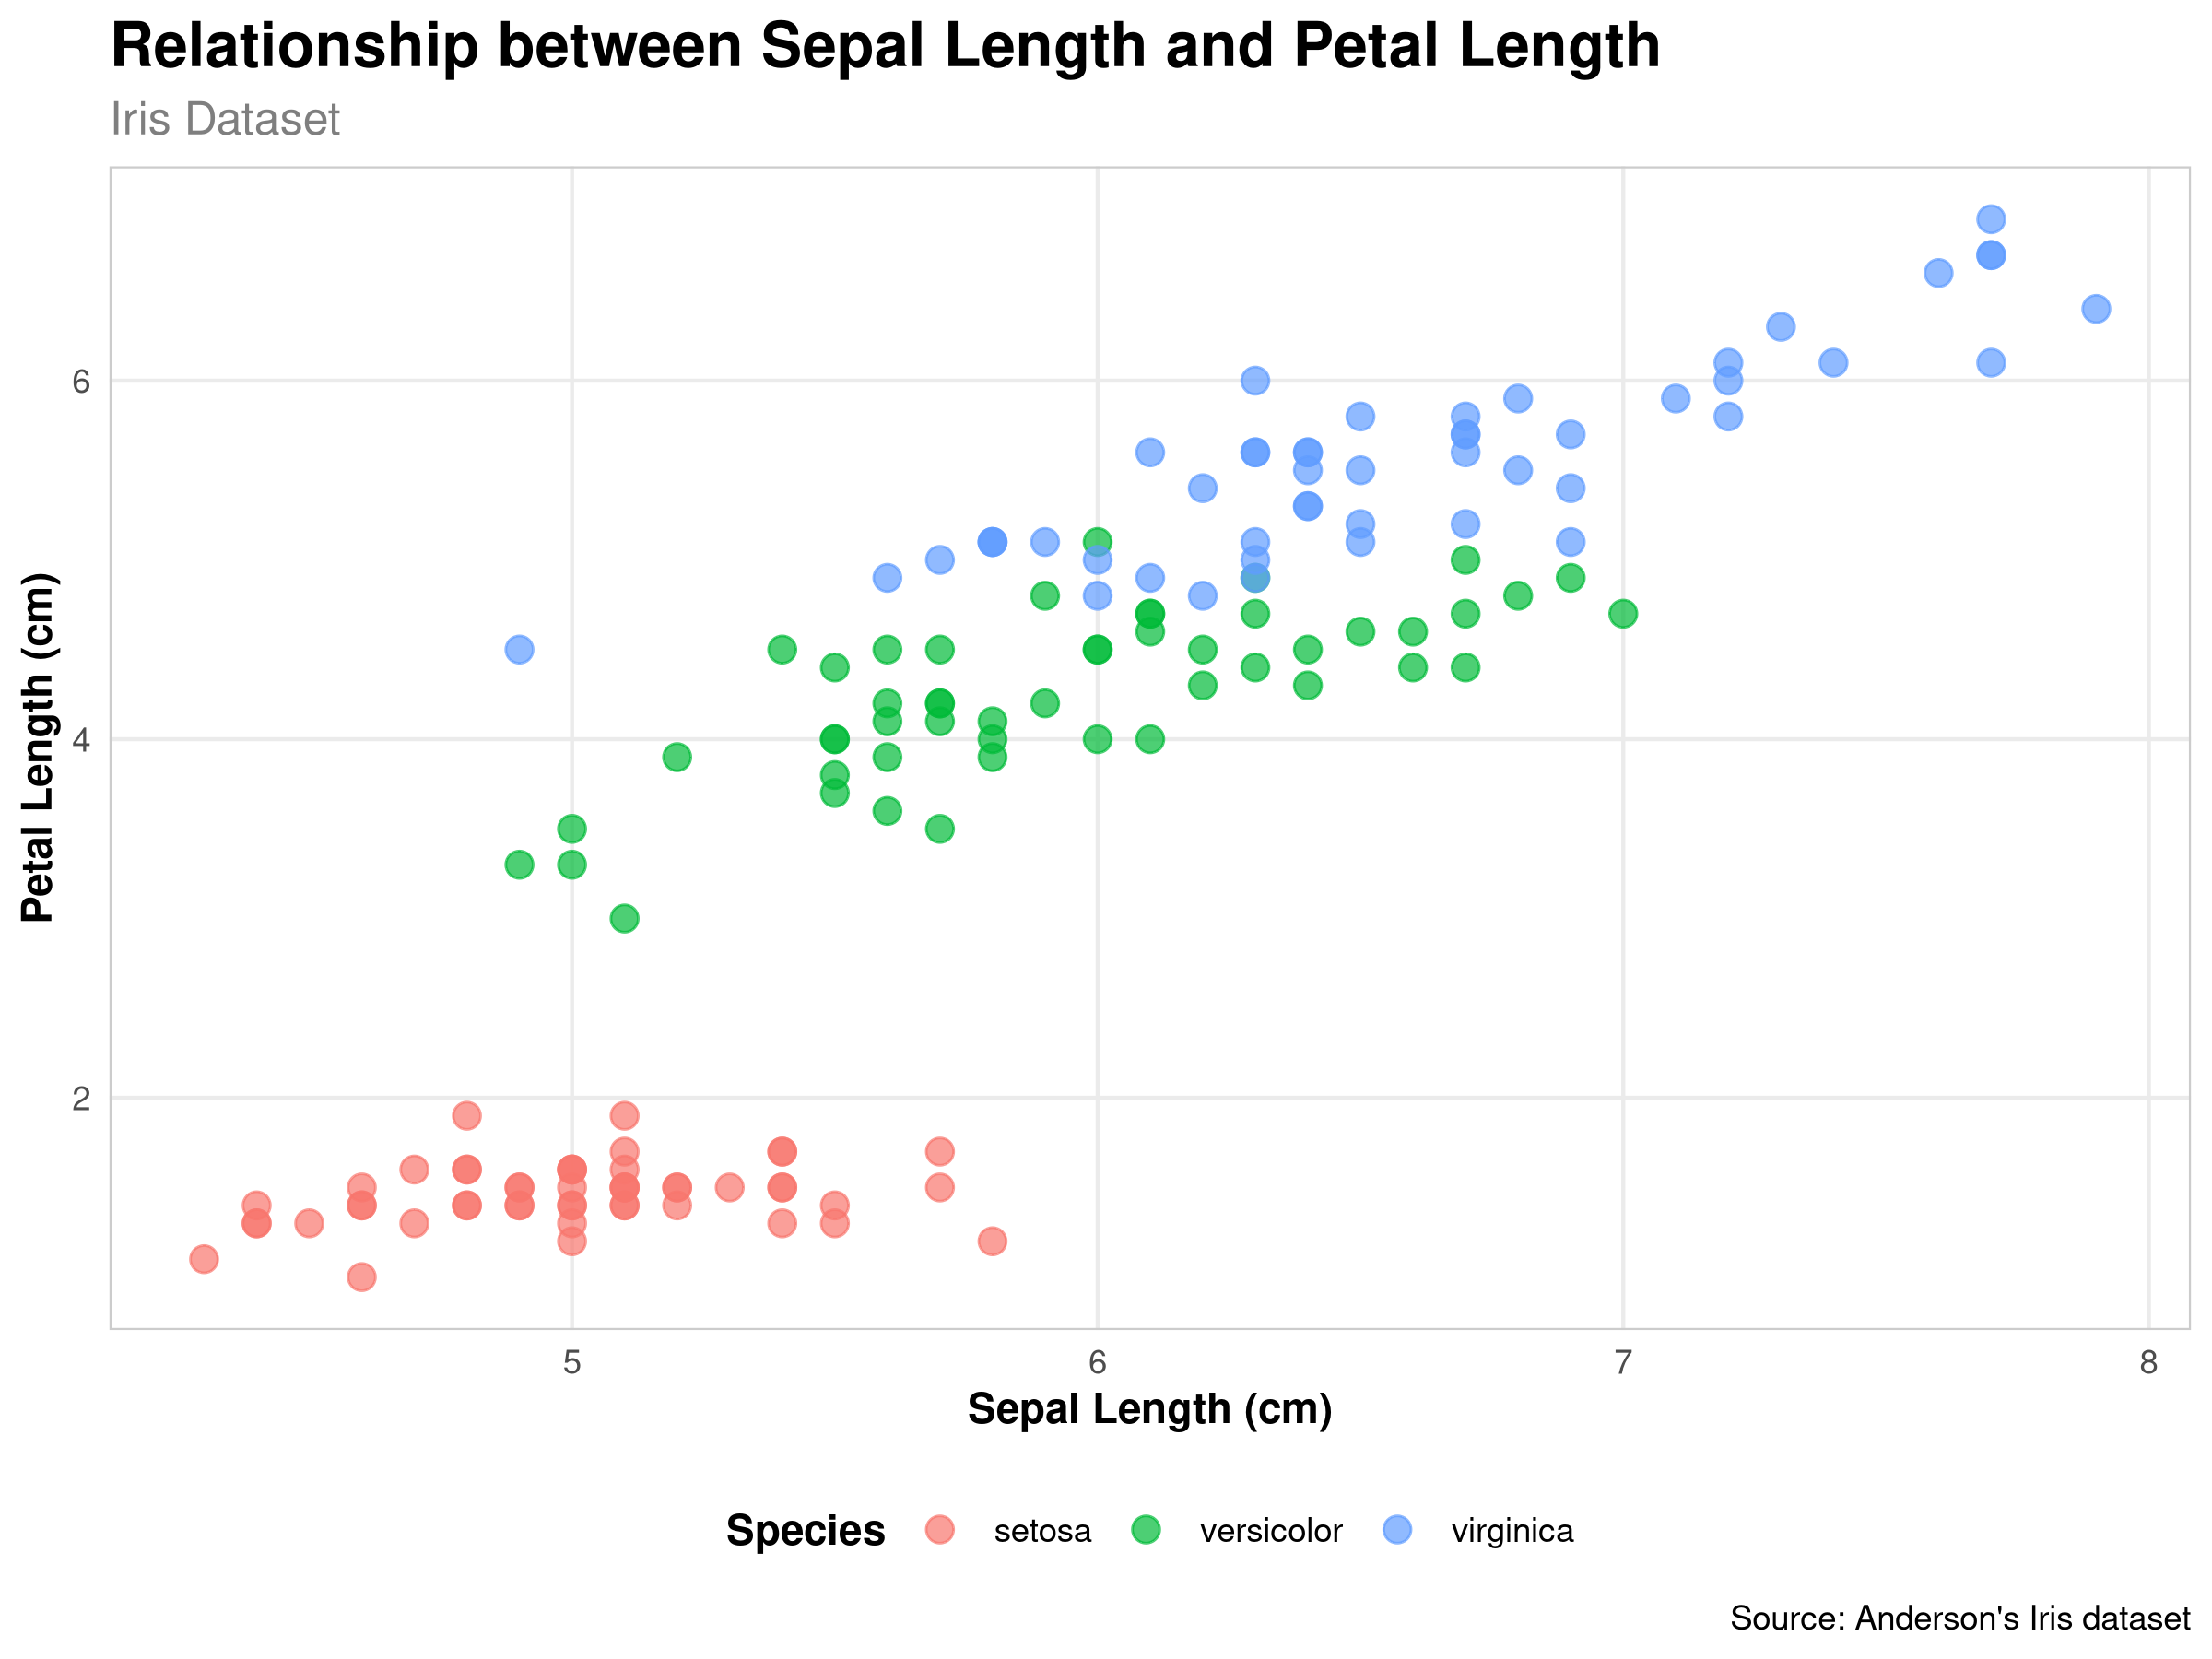
\includegraphics[keepaspectratio]{chapters/07-advanced-visualization_files/figure-pdf/unnamed-chunk-1-2.pdf}}

\subsection{Color Palettes for Ecological
Data}\label{color-palettes-for-ecological-data}

Choosing appropriate color palettes is crucial for effective
visualization:

\begin{Shaded}
\begin{Highlighting}[]
\CommentTok{\# Load packages for color palettes}
\FunctionTok{library}\NormalTok{(RColorBrewer)}
\FunctionTok{library}\NormalTok{(viridis)}

\CommentTok{\# Display color palettes suitable for ecological data}
\FunctionTok{par}\NormalTok{(}\AttributeTok{mfrow =} \FunctionTok{c}\NormalTok{(}\DecValTok{4}\NormalTok{, }\DecValTok{1}\NormalTok{), }\AttributeTok{mar =} \FunctionTok{c}\NormalTok{(}\DecValTok{2}\NormalTok{, }\DecValTok{6}\NormalTok{, }\DecValTok{2}\NormalTok{, }\DecValTok{1}\NormalTok{))}
\FunctionTok{display.brewer.pal}\NormalTok{(}\DecValTok{8}\NormalTok{, }\StringTok{"YlGn"}\NormalTok{)}
\FunctionTok{display.brewer.pal}\NormalTok{(}\DecValTok{8}\NormalTok{, }\StringTok{"BrBG"}\NormalTok{)}
\FunctionTok{display.brewer.pal}\NormalTok{(}\DecValTok{11}\NormalTok{, }\StringTok{"RdYlBu"}\NormalTok{)}
\NormalTok{scales}\SpecialCharTok{::}\FunctionTok{show\_col}\NormalTok{(}\FunctionTok{viridis}\NormalTok{(}\DecValTok{8}\NormalTok{))}
\end{Highlighting}
\end{Shaded}

\pandocbounded{\includegraphics[keepaspectratio]{chapters/07-advanced-visualization_files/figure-pdf/unnamed-chunk-2-1.pdf}}

\begin{Shaded}
\begin{Highlighting}[]
\CommentTok{\# Apply different color palettes to our plot}
\NormalTok{plot1 }\OtherTok{\textless{}{-}}\NormalTok{ base\_plot }\SpecialCharTok{+} 
  \FunctionTok{scale\_color\_brewer}\NormalTok{(}\AttributeTok{palette =} \StringTok{"Set1"}\NormalTok{) }\SpecialCharTok{+}
\NormalTok{  custom\_theme }\SpecialCharTok{+}
  \FunctionTok{ggtitle}\NormalTok{(}\StringTok{"Color Brewer \textquotesingle{}Set1\textquotesingle{} Palette"}\NormalTok{)}

\NormalTok{plot2 }\OtherTok{\textless{}{-}}\NormalTok{ base\_plot }\SpecialCharTok{+} 
  \FunctionTok{scale\_color\_viridis\_d}\NormalTok{() }\SpecialCharTok{+}
\NormalTok{  custom\_theme }\SpecialCharTok{+}
  \FunctionTok{ggtitle}\NormalTok{(}\StringTok{"Viridis Discrete Palette"}\NormalTok{)}

\CommentTok{\# Display the plots}
\NormalTok{plot1}
\end{Highlighting}
\end{Shaded}

\pandocbounded{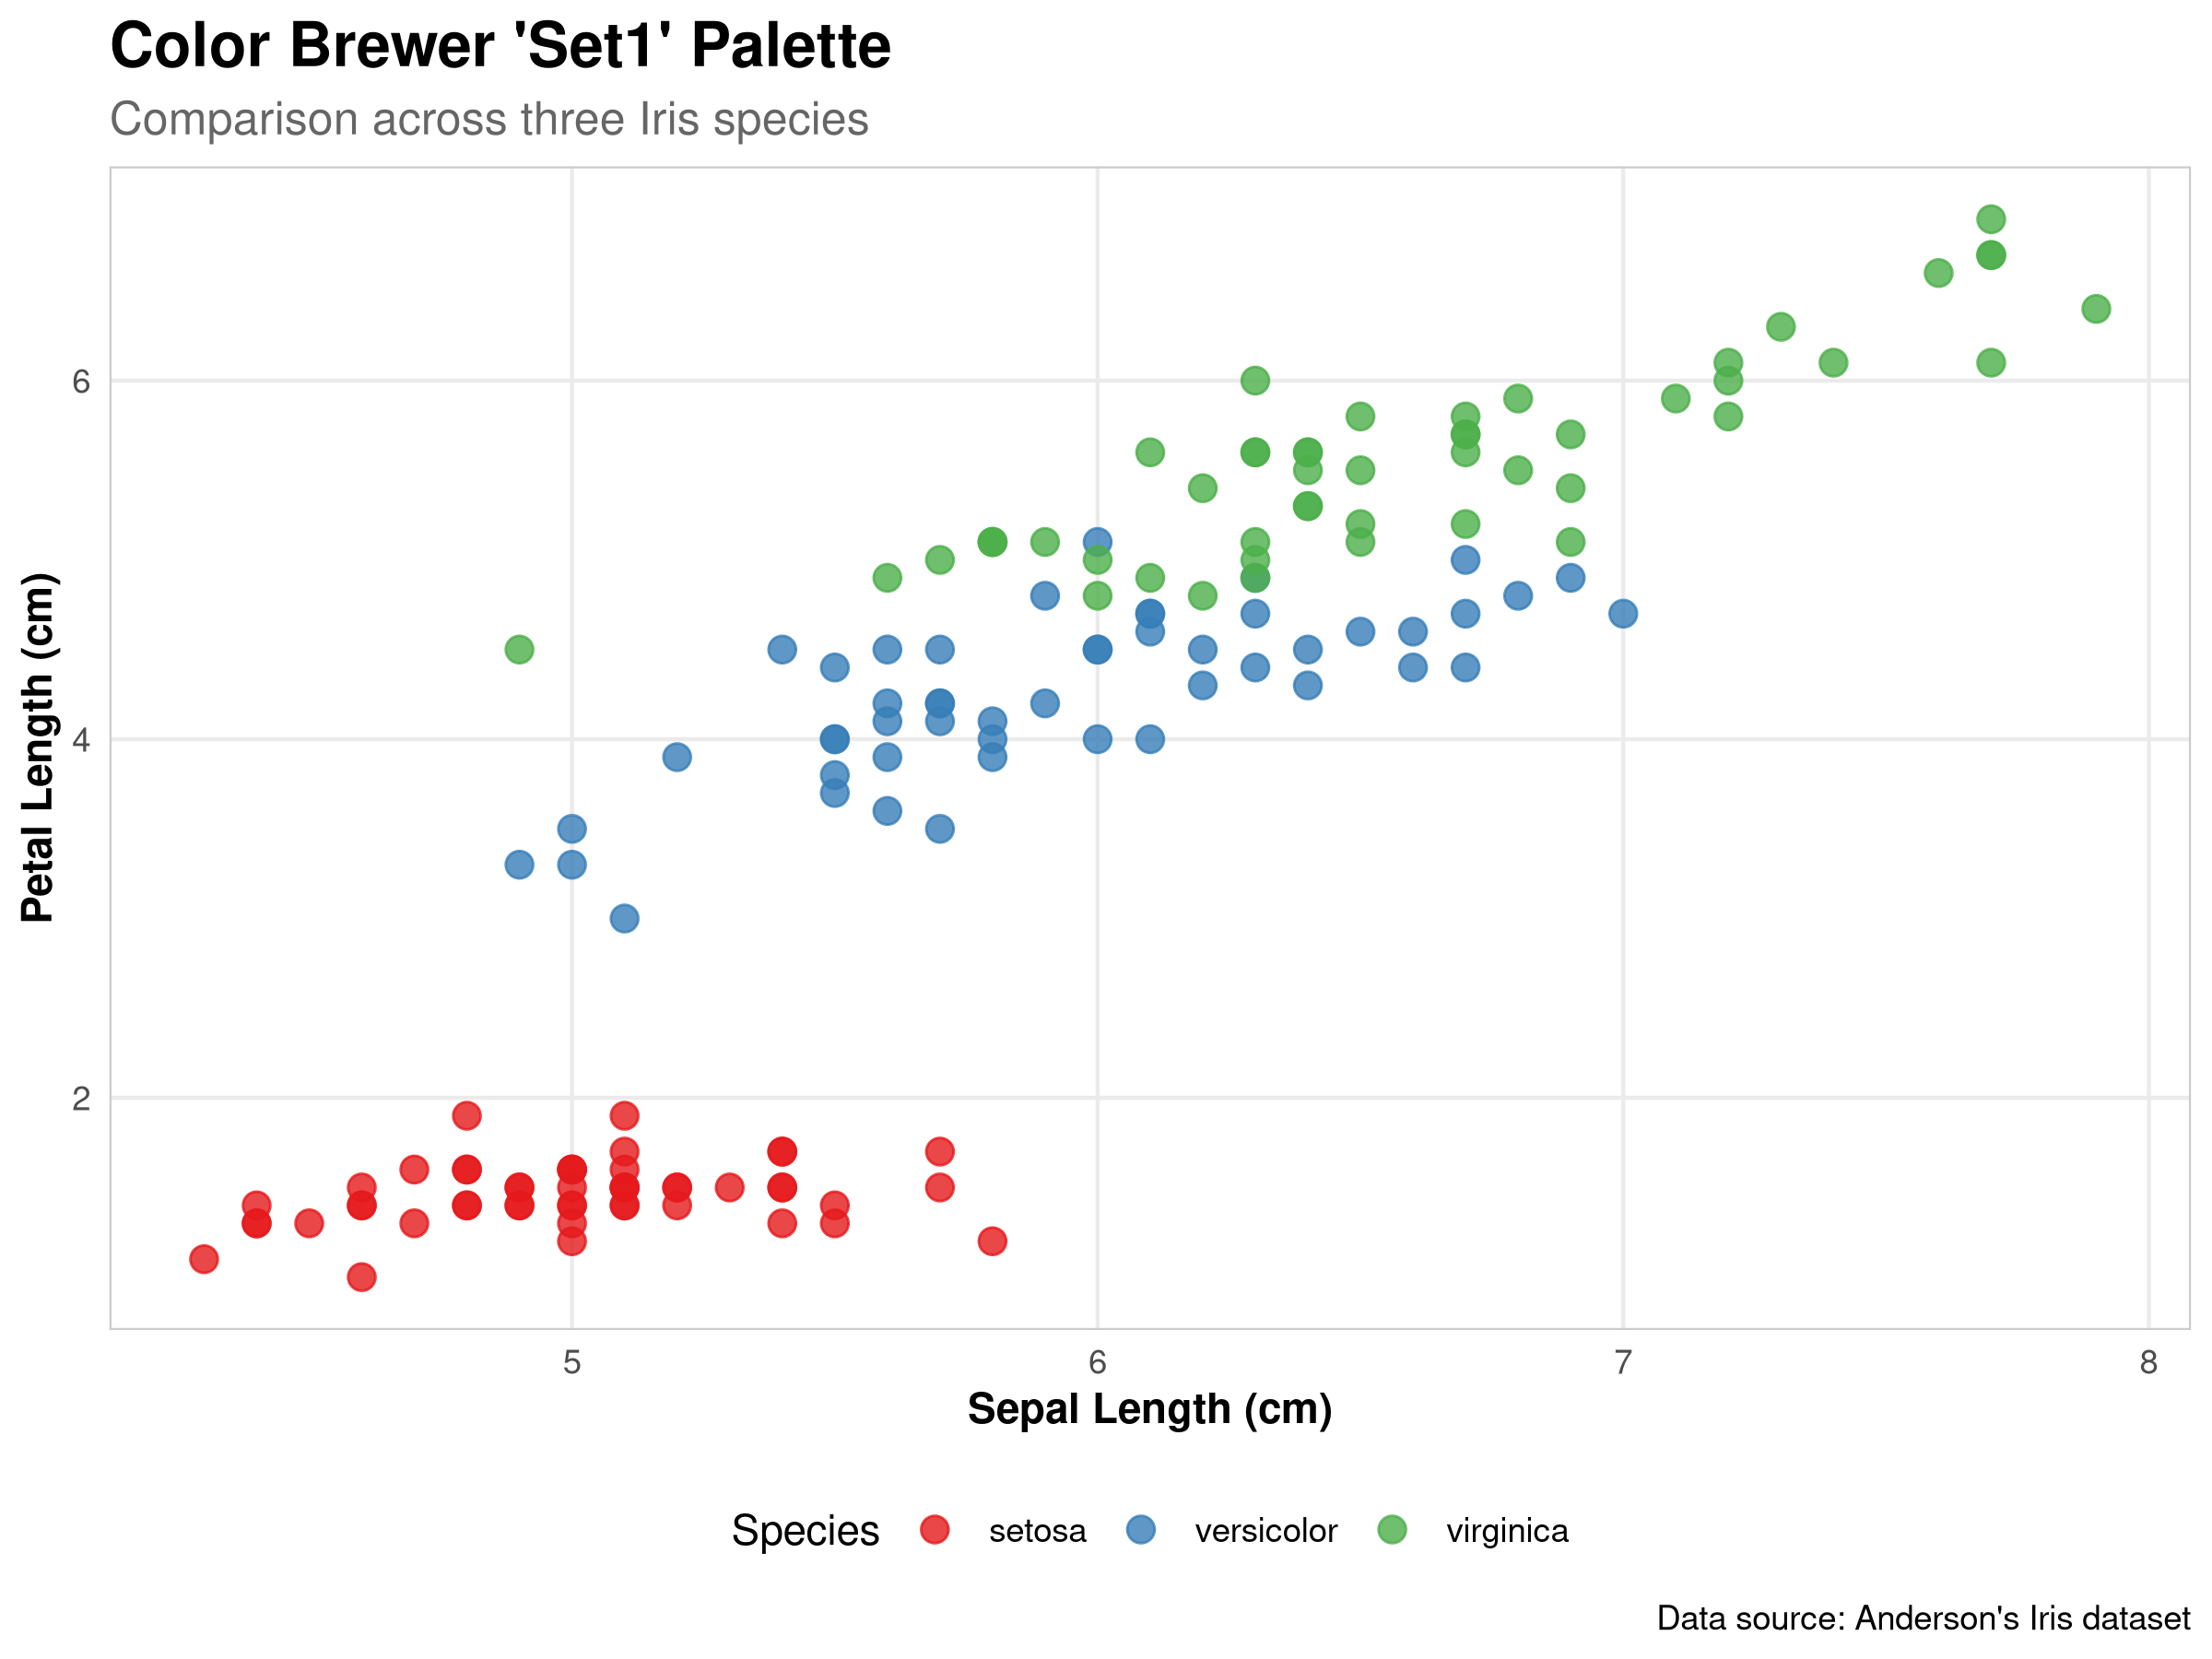
\includegraphics[keepaspectratio]{chapters/07-advanced-visualization_files/figure-pdf/unnamed-chunk-2-2.pdf}}

\begin{Shaded}
\begin{Highlighting}[]
\NormalTok{plot2}
\end{Highlighting}
\end{Shaded}

\pandocbounded{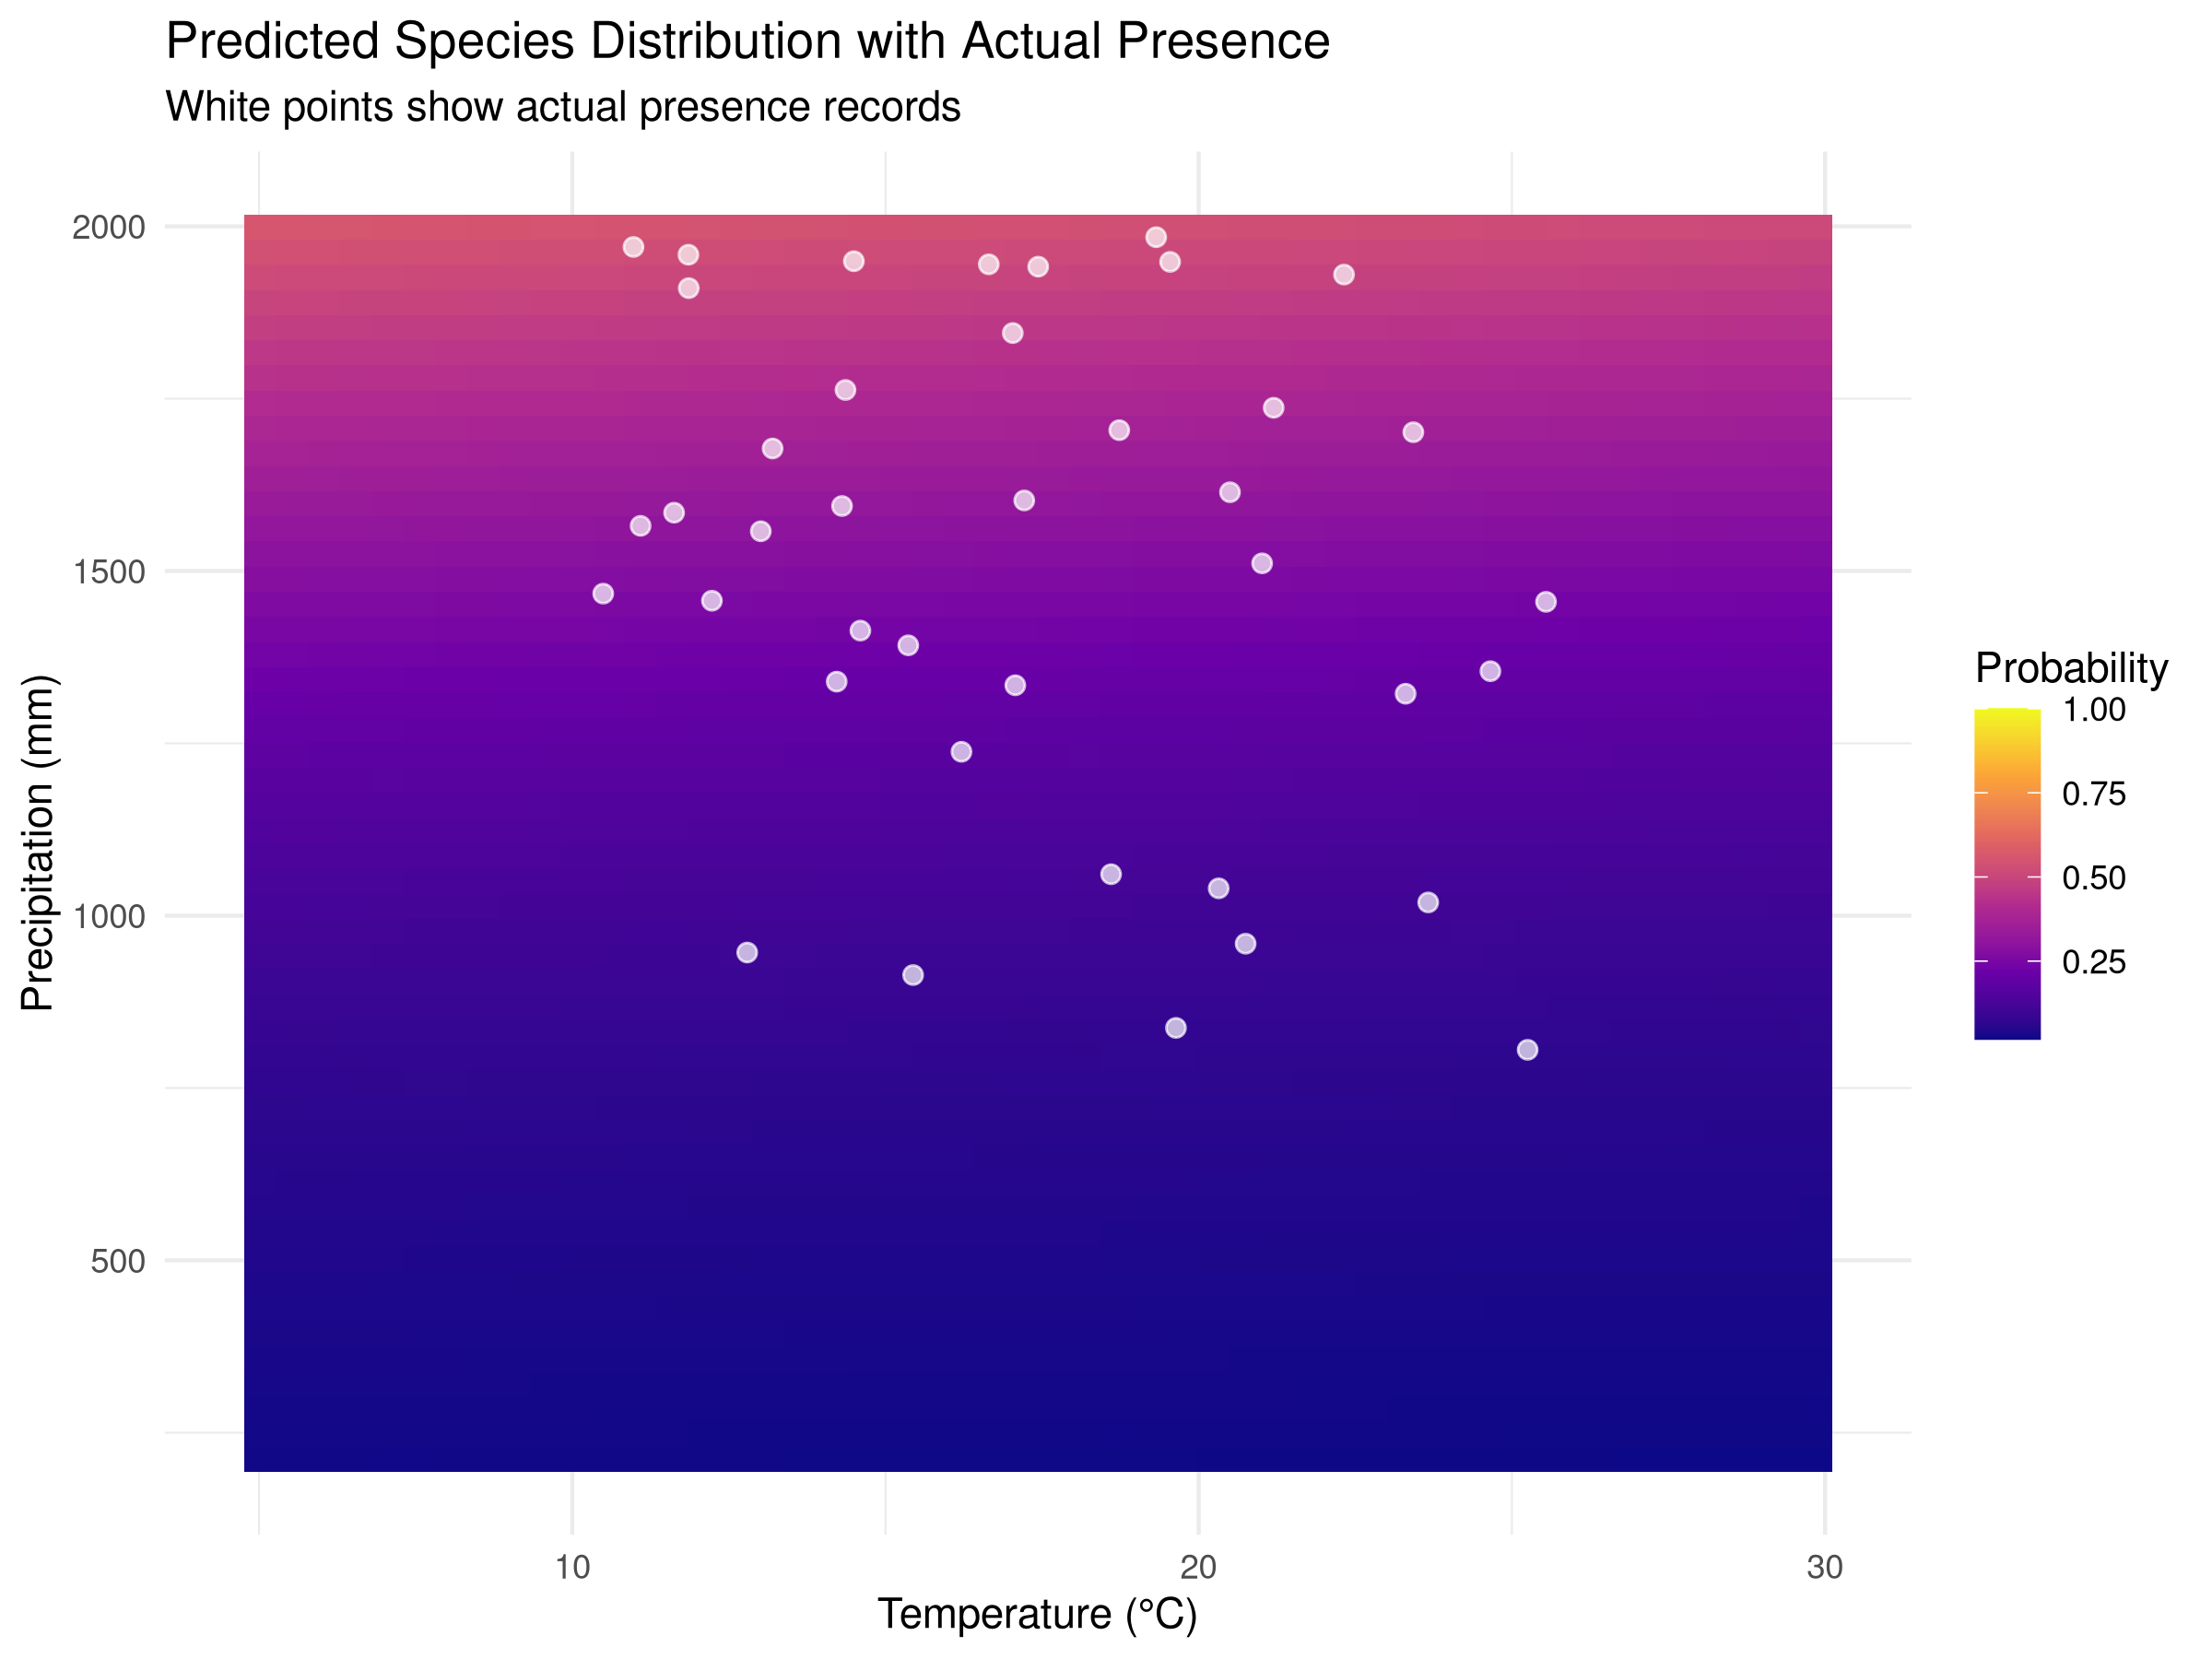
\includegraphics[keepaspectratio]{chapters/07-advanced-visualization_files/figure-pdf/unnamed-chunk-2-3.pdf}}

\subsection{Arranging Multiple Plots}\label{arranging-multiple-plots}

Combining multiple plots can help compare different aspects of your
data:

\begin{Shaded}
\begin{Highlighting}[]
\FunctionTok{library}\NormalTok{(patchwork)}

\CommentTok{\# Create individual plots}
\NormalTok{p1 }\OtherTok{\textless{}{-}} \FunctionTok{ggplot}\NormalTok{(iris, }\FunctionTok{aes}\NormalTok{(}\AttributeTok{x =}\NormalTok{ Species, }\AttributeTok{y =}\NormalTok{ Sepal.Length, }\AttributeTok{fill =}\NormalTok{ Species)) }\SpecialCharTok{+}
  \FunctionTok{geom\_boxplot}\NormalTok{() }\SpecialCharTok{+}
  \FunctionTok{labs}\NormalTok{(}\AttributeTok{title =} \StringTok{"Sepal Length by Species"}\NormalTok{,}
       \AttributeTok{x =} \ConstantTok{NULL}\NormalTok{,}
       \AttributeTok{y =} \StringTok{"Sepal Length (cm)"}\NormalTok{) }\SpecialCharTok{+}
  \FunctionTok{theme\_minimal}\NormalTok{() }\SpecialCharTok{+}
  \FunctionTok{theme}\NormalTok{(}\AttributeTok{legend.position =} \StringTok{"none"}\NormalTok{)}

\NormalTok{p2 }\OtherTok{\textless{}{-}} \FunctionTok{ggplot}\NormalTok{(iris, }\FunctionTok{aes}\NormalTok{(}\AttributeTok{x =}\NormalTok{ Species, }\AttributeTok{y =}\NormalTok{ Petal.Length, }\AttributeTok{fill =}\NormalTok{ Species)) }\SpecialCharTok{+}
  \FunctionTok{geom\_boxplot}\NormalTok{() }\SpecialCharTok{+}
  \FunctionTok{labs}\NormalTok{(}\AttributeTok{title =} \StringTok{"Petal Length by Species"}\NormalTok{,}
       \AttributeTok{x =} \ConstantTok{NULL}\NormalTok{,}
       \AttributeTok{y =} \StringTok{"Petal Length (cm)"}\NormalTok{) }\SpecialCharTok{+}
  \FunctionTok{theme\_minimal}\NormalTok{() }\SpecialCharTok{+}
  \FunctionTok{theme}\NormalTok{(}\AttributeTok{legend.position =} \StringTok{"none"}\NormalTok{)}

\NormalTok{p3 }\OtherTok{\textless{}{-}} \FunctionTok{ggplot}\NormalTok{(iris, }\FunctionTok{aes}\NormalTok{(}\AttributeTok{x =}\NormalTok{ Sepal.Length, }\AttributeTok{fill =}\NormalTok{ Species)) }\SpecialCharTok{+}
  \FunctionTok{geom\_density}\NormalTok{(}\AttributeTok{alpha =} \FloatTok{0.7}\NormalTok{) }\SpecialCharTok{+}
  \FunctionTok{labs}\NormalTok{(}\AttributeTok{title =} \StringTok{"Sepal Length Distribution"}\NormalTok{,}
       \AttributeTok{x =} \StringTok{"Sepal Length (cm)"}\NormalTok{,}
       \AttributeTok{y =} \StringTok{"Density"}\NormalTok{) }\SpecialCharTok{+}
  \FunctionTok{theme\_minimal}\NormalTok{()}

\NormalTok{p4 }\OtherTok{\textless{}{-}} \FunctionTok{ggplot}\NormalTok{(iris, }\FunctionTok{aes}\NormalTok{(}\AttributeTok{x =}\NormalTok{ Petal.Length, }\AttributeTok{fill =}\NormalTok{ Species)) }\SpecialCharTok{+}
  \FunctionTok{geom\_density}\NormalTok{(}\AttributeTok{alpha =} \FloatTok{0.7}\NormalTok{) }\SpecialCharTok{+}
  \FunctionTok{labs}\NormalTok{(}\AttributeTok{title =} \StringTok{"Petal Length Distribution"}\NormalTok{,}
       \AttributeTok{x =} \StringTok{"Petal Length (cm)"}\NormalTok{,}
       \AttributeTok{y =} \StringTok{"Density"}\NormalTok{) }\SpecialCharTok{+}
  \FunctionTok{theme\_minimal}\NormalTok{()}

\CommentTok{\# Arrange the plots}
\NormalTok{(p1 }\SpecialCharTok{+}\NormalTok{ p2) }\SpecialCharTok{/}\NormalTok{ (p3 }\SpecialCharTok{+}\NormalTok{ p4) }\SpecialCharTok{+} 
  \FunctionTok{plot\_annotation}\NormalTok{(}
    \AttributeTok{title =} \StringTok{"Iris Morphology by Species"}\NormalTok{,}
    \AttributeTok{caption =} \StringTok{"Source: Anderson\textquotesingle{}s Iris dataset"}
\NormalTok{  )}
\end{Highlighting}
\end{Shaded}

\pandocbounded{\includegraphics[keepaspectratio]{chapters/07-advanced-visualization_files/figure-pdf/unnamed-chunk-3-1.pdf}}

\section{Interactive Visualizations}\label{interactive-visualizations}

\subsection{Creating Interactive Plots with
plotly}\label{creating-interactive-plots-with-plotly}

Interactive plots allow users to explore data more deeply:

\begin{Shaded}
\begin{Highlighting}[]
\FunctionTok{library}\NormalTok{(plotly)}
\FunctionTok{library}\NormalTok{(knitr)}

\CommentTok{\# Create a ggplot visualization}
\NormalTok{p }\OtherTok{\textless{}{-}} \FunctionTok{ggplot}\NormalTok{(iris, }\FunctionTok{aes}\NormalTok{(}\AttributeTok{x =}\NormalTok{ Sepal.Length, }\AttributeTok{y =}\NormalTok{ Petal.Length, }\AttributeTok{color =}\NormalTok{ Species)) }\SpecialCharTok{+}
  \FunctionTok{geom\_point}\NormalTok{(}\AttributeTok{size =} \DecValTok{3}\NormalTok{, }\AttributeTok{alpha =} \FloatTok{0.7}\NormalTok{) }\SpecialCharTok{+}
  \FunctionTok{labs}\NormalTok{(}\AttributeTok{title =} \StringTok{"Relationship between Sepal Length and Petal Length"}\NormalTok{,}
       \AttributeTok{x =} \StringTok{"Sepal Length (cm)"}\NormalTok{,}
       \AttributeTok{y =} \StringTok{"Petal Length (cm)"}\NormalTok{) }\SpecialCharTok{+}
  \FunctionTok{theme\_minimal}\NormalTok{() }\SpecialCharTok{+}
  \FunctionTok{scale\_color\_viridis\_d}\NormalTok{()}

\CommentTok{\# Check if we\textquotesingle{}re in HTML output mode}
\ControlFlowTok{if}\NormalTok{ (knitr}\SpecialCharTok{::}\FunctionTok{is\_html\_output}\NormalTok{()) \{}
  \CommentTok{\# For HTML output, use the interactive plotly version}
  \FunctionTok{ggplotly}\NormalTok{(p)}
\NormalTok{\} }\ControlFlowTok{else}\NormalTok{ \{}
  \CommentTok{\# For PDF output, use the static ggplot version}
\NormalTok{  p }\SpecialCharTok{+} \FunctionTok{annotate}\NormalTok{(}\StringTok{"text"}\NormalTok{, }\AttributeTok{x =} \DecValTok{6}\NormalTok{, }\AttributeTok{y =} \DecValTok{6}\NormalTok{, }
               \AttributeTok{label =} \StringTok{"Note: Interactive version available in HTML output"}\NormalTok{, }
               \AttributeTok{fontface =} \StringTok{"italic"}\NormalTok{, }\AttributeTok{size =} \DecValTok{3}\NormalTok{)}
\NormalTok{\}}
\end{Highlighting}
\end{Shaded}

\begin{figure}[H]

{\centering \pandocbounded{\includegraphics[keepaspectratio]{chapters/07-advanced-visualization_files/figure-pdf/interactive-plotly-1.pdf}}

}

\caption{Relationship between Sepal Length and Petal Length across
different Iris species. In the HTML version, this plot is interactive
and allows zooming, panning, and hovering for details.}

\end{figure}%

\subsection{Interactive Maps with
leaflet}\label{interactive-maps-with-leaflet}

For spatial ecological data, interactive maps can be particularly
useful:

\begin{Shaded}
\begin{Highlighting}[]
\FunctionTok{library}\NormalTok{(leaflet)}
\FunctionTok{library}\NormalTok{(ggplot2)}
\FunctionTok{library}\NormalTok{(knitr)}

\CommentTok{\# Create sample ecological site data}
\NormalTok{sites }\OtherTok{\textless{}{-}} \FunctionTok{data.frame}\NormalTok{(}
  \AttributeTok{name =} \FunctionTok{c}\NormalTok{(}\StringTok{"Forest Reserve"}\NormalTok{, }\StringTok{"Wetland Study Area"}\NormalTok{, }\StringTok{"Grassland Transect"}\NormalTok{, }
           \StringTok{"Mountain Research Station"}\NormalTok{, }\StringTok{"Coastal Monitoring Site"}\NormalTok{),}
  \AttributeTok{lat =} \FunctionTok{c}\NormalTok{(}\FloatTok{37.7749}\NormalTok{, }\FloatTok{37.8}\NormalTok{, }\FloatTok{37.75}\NormalTok{, }\FloatTok{37.85}\NormalTok{, }\FloatTok{37.7}\NormalTok{),}
  \AttributeTok{lng =} \FunctionTok{c}\NormalTok{(}\SpecialCharTok{{-}}\FloatTok{122.4194}\NormalTok{, }\SpecialCharTok{{-}}\FloatTok{122.45}\NormalTok{, }\SpecialCharTok{{-}}\FloatTok{122.5}\NormalTok{, }\SpecialCharTok{{-}}\FloatTok{122.4}\NormalTok{, }\SpecialCharTok{{-}}\FloatTok{122.3}\NormalTok{),}
  \AttributeTok{habitat =} \FunctionTok{c}\NormalTok{(}\StringTok{"Forest"}\NormalTok{, }\StringTok{"Wetland"}\NormalTok{, }\StringTok{"Grassland"}\NormalTok{, }\StringTok{"Alpine"}\NormalTok{, }\StringTok{"Coastal"}\NormalTok{),}
  \AttributeTok{species\_count =} \FunctionTok{c}\NormalTok{(}\DecValTok{120}\NormalTok{, }\DecValTok{85}\NormalTok{, }\DecValTok{65}\NormalTok{, }\DecValTok{95}\NormalTok{, }\DecValTok{110}\NormalTok{)}
\NormalTok{)}

\CommentTok{\# Create a color palette based on habitat type}
\NormalTok{habitat\_colors }\OtherTok{\textless{}{-}} \FunctionTok{c}\NormalTok{(}\StringTok{"darkgreen"}\NormalTok{, }\StringTok{"blue"}\NormalTok{, }\StringTok{"gold"}\NormalTok{, }\StringTok{"purple"}\NormalTok{, }\StringTok{"lightblue"}\NormalTok{)}
\FunctionTok{names}\NormalTok{(habitat\_colors) }\OtherTok{\textless{}{-}} \FunctionTok{c}\NormalTok{(}\StringTok{"Forest"}\NormalTok{, }\StringTok{"Wetland"}\NormalTok{, }\StringTok{"Grassland"}\NormalTok{, }\StringTok{"Alpine"}\NormalTok{, }\StringTok{"Coastal"}\NormalTok{)}

\ControlFlowTok{if}\NormalTok{ (knitr}\SpecialCharTok{::}\FunctionTok{is\_html\_output}\NormalTok{()) \{}
  \CommentTok{\# For HTML output, create an interactive leaflet map}
\NormalTok{  habitat\_pal }\OtherTok{\textless{}{-}} \FunctionTok{colorFactor}\NormalTok{(}
    \AttributeTok{palette =}\NormalTok{ habitat\_colors,}
    \AttributeTok{domain =}\NormalTok{ sites}\SpecialCharTok{$}\NormalTok{habitat}
\NormalTok{  )}
  
  \CommentTok{\# Create an interactive map}
  \FunctionTok{leaflet}\NormalTok{(sites) }\SpecialCharTok{\%\textgreater{}\%}
    \FunctionTok{addTiles}\NormalTok{() }\SpecialCharTok{\%\textgreater{}\%}  \CommentTok{\# Add default OpenStreetMap tiles}
    \FunctionTok{addCircleMarkers}\NormalTok{(}
      \SpecialCharTok{\textasciitilde{}}\NormalTok{lng, }\SpecialCharTok{\textasciitilde{}}\NormalTok{lat,}
      \AttributeTok{color =} \SpecialCharTok{\textasciitilde{}}\FunctionTok{habitat\_pal}\NormalTok{(habitat),}
      \AttributeTok{radius =} \SpecialCharTok{\textasciitilde{}}\FunctionTok{sqrt}\NormalTok{(species\_count) }\SpecialCharTok{*} \FloatTok{1.5}\NormalTok{,}
      \AttributeTok{popup =} \SpecialCharTok{\textasciitilde{}}\FunctionTok{paste}\NormalTok{(}\StringTok{"\textless{}b\textgreater{}"}\NormalTok{, name, }\StringTok{"\textless{}/b\textgreater{}\textless{}br\textgreater{}"}\NormalTok{,}
                     \StringTok{"Habitat: "}\NormalTok{, habitat, }\StringTok{"\textless{}br\textgreater{}"}\NormalTok{,}
                     \StringTok{"Species Count: "}\NormalTok{, species\_count),}
      \AttributeTok{label =} \SpecialCharTok{\textasciitilde{}}\NormalTok{name,}
      \AttributeTok{fillOpacity =} \FloatTok{0.7}
\NormalTok{    ) }\SpecialCharTok{\%\textgreater{}\%}
    \FunctionTok{addLegend}\NormalTok{(}
      \AttributeTok{position =} \StringTok{"bottomright"}\NormalTok{,}
      \AttributeTok{pal =}\NormalTok{ habitat\_pal,}
      \AttributeTok{values =} \SpecialCharTok{\textasciitilde{}}\NormalTok{habitat,}
      \AttributeTok{title =} \StringTok{"Habitat Type"}\NormalTok{,}
      \AttributeTok{opacity =} \FloatTok{0.7}
\NormalTok{    )}
\NormalTok{\} }\ControlFlowTok{else}\NormalTok{ \{}
  \CommentTok{\# For PDF output, create a static ggplot map}
\NormalTok{  world }\OtherTok{\textless{}{-}} \FunctionTok{map\_data}\NormalTok{(}\StringTok{"world"}\NormalTok{)}
  
  \FunctionTok{ggplot}\NormalTok{() }\SpecialCharTok{+}
    \FunctionTok{geom\_polygon}\NormalTok{(}\AttributeTok{data =}\NormalTok{ world, }\FunctionTok{aes}\NormalTok{(}\AttributeTok{x =}\NormalTok{ long, }\AttributeTok{y =}\NormalTok{ lat, }\AttributeTok{group =}\NormalTok{ group), }
                 \AttributeTok{fill =} \StringTok{"lightgray"}\NormalTok{, }\AttributeTok{color =} \StringTok{"darkgray"}\NormalTok{, }\AttributeTok{size =} \FloatTok{0.2}\NormalTok{) }\SpecialCharTok{+}
    \FunctionTok{geom\_point}\NormalTok{(}\AttributeTok{data =}\NormalTok{ sites, }\FunctionTok{aes}\NormalTok{(}\AttributeTok{x =}\NormalTok{ lng, }\AttributeTok{y =}\NormalTok{ lat, }\AttributeTok{color =}\NormalTok{ habitat, }\AttributeTok{size =}\NormalTok{ species\_count),}
               \AttributeTok{alpha =} \FloatTok{0.7}\NormalTok{) }\SpecialCharTok{+}
    \FunctionTok{scale\_color\_manual}\NormalTok{(}\AttributeTok{values =}\NormalTok{ habitat\_colors) }\SpecialCharTok{+}
    \FunctionTok{scale\_size\_continuous}\NormalTok{(}\AttributeTok{range =} \FunctionTok{c}\NormalTok{(}\DecValTok{3}\NormalTok{, }\DecValTok{8}\NormalTok{), }\AttributeTok{name =} \StringTok{"Species Count"}\NormalTok{) }\SpecialCharTok{+}
    \FunctionTok{coord\_fixed}\NormalTok{(}\AttributeTok{xlim =} \FunctionTok{c}\NormalTok{(}\SpecialCharTok{{-}}\DecValTok{123}\NormalTok{, }\SpecialCharTok{{-}}\DecValTok{122}\NormalTok{), }\AttributeTok{ylim =} \FunctionTok{c}\NormalTok{(}\FloatTok{37.6}\NormalTok{, }\FloatTok{37.9}\NormalTok{)) }\SpecialCharTok{+}
    \FunctionTok{labs}\NormalTok{(}\AttributeTok{title =} \StringTok{"Ecological Study Sites"}\NormalTok{,}
         \AttributeTok{subtitle =} \StringTok{"Note: Interactive version available in HTML output"}\NormalTok{,}
         \AttributeTok{x =} \StringTok{"Longitude"}\NormalTok{, }\AttributeTok{y =} \StringTok{"Latitude"}\NormalTok{, }\AttributeTok{color =} \StringTok{"Habitat Type"}\NormalTok{) }\SpecialCharTok{+}
    \FunctionTok{theme\_minimal}\NormalTok{() }\SpecialCharTok{+}
    \FunctionTok{theme}\NormalTok{(}\AttributeTok{legend.position =} \StringTok{"right"}\NormalTok{)}
\NormalTok{\}}
\end{Highlighting}
\end{Shaded}

\begin{figure}[H]

{\centering \pandocbounded{\includegraphics[keepaspectratio]{chapters/07-advanced-visualization_files/figure-pdf/interactive-map-1.pdf}}

}

\caption{Ecological study sites across different habitat types. In the
HTML version, this map is interactive and allows zooming, panning, and
clicking on markers for details.}

\end{figure}%

\section{Specialized Ecological
Visualizations}\label{specialized-ecological-visualizations}

\subsection{Ordination Plots}\label{ordination-plots}

Ordination techniques like PCA and NMDS are common in ecological
studies:

\begin{Shaded}
\begin{Highlighting}[]
\CommentTok{\# Perform PCA on iris dataset}
\NormalTok{pca\_result }\OtherTok{\textless{}{-}} \FunctionTok{prcomp}\NormalTok{(iris[, }\DecValTok{1}\SpecialCharTok{:}\DecValTok{4}\NormalTok{], }\AttributeTok{scale. =} \ConstantTok{TRUE}\NormalTok{)}
\NormalTok{pca\_data }\OtherTok{\textless{}{-}} \FunctionTok{as.data.frame}\NormalTok{(pca\_result}\SpecialCharTok{$}\NormalTok{x)}
\NormalTok{pca\_data}\SpecialCharTok{$}\NormalTok{Species }\OtherTok{\textless{}{-}}\NormalTok{ iris}\SpecialCharTok{$}\NormalTok{Species}

\CommentTok{\# Create a PCA biplot}
\FunctionTok{ggplot}\NormalTok{(pca\_data, }\FunctionTok{aes}\NormalTok{(}\AttributeTok{x =}\NormalTok{ PC1, }\AttributeTok{y =}\NormalTok{ PC2, }\AttributeTok{color =}\NormalTok{ Species)) }\SpecialCharTok{+}
  \FunctionTok{geom\_point}\NormalTok{(}\AttributeTok{size =} \DecValTok{3}\NormalTok{, }\AttributeTok{alpha =} \FloatTok{0.7}\NormalTok{) }\SpecialCharTok{+}
  \FunctionTok{stat\_ellipse}\NormalTok{(}\AttributeTok{level =} \FloatTok{0.95}\NormalTok{) }\SpecialCharTok{+}
  \FunctionTok{labs}\NormalTok{(}\AttributeTok{title =} \StringTok{"PCA of Iris Dataset"}\NormalTok{,}
       \AttributeTok{x =} \FunctionTok{paste0}\NormalTok{(}\StringTok{"PC1 ("}\NormalTok{, }\FunctionTok{round}\NormalTok{(}\FunctionTok{summary}\NormalTok{(pca\_result)}\SpecialCharTok{$}\NormalTok{importance[}\DecValTok{2}\NormalTok{, }\DecValTok{1}\NormalTok{] }\SpecialCharTok{*} \DecValTok{100}\NormalTok{, }\DecValTok{1}\NormalTok{), }\StringTok{"\%)"}\NormalTok{),}
       \AttributeTok{y =} \FunctionTok{paste0}\NormalTok{(}\StringTok{"PC2 ("}\NormalTok{, }\FunctionTok{round}\NormalTok{(}\FunctionTok{summary}\NormalTok{(pca\_result)}\SpecialCharTok{$}\NormalTok{importance[}\DecValTok{2}\NormalTok{, }\DecValTok{2}\NormalTok{] }\SpecialCharTok{*} \DecValTok{100}\NormalTok{, }\DecValTok{1}\NormalTok{), }\StringTok{"\%)"}\NormalTok{)) }\SpecialCharTok{+}
  \FunctionTok{theme\_minimal}\NormalTok{()}
\end{Highlighting}
\end{Shaded}

\pandocbounded{\includegraphics[keepaspectratio]{chapters/07-advanced-visualization_files/figure-pdf/unnamed-chunk-4-1.pdf}}

\begin{Shaded}
\begin{Highlighting}[]
\CommentTok{\# Create a loadings plot}
\NormalTok{loadings }\OtherTok{\textless{}{-}} \FunctionTok{as.data.frame}\NormalTok{(pca\_result}\SpecialCharTok{$}\NormalTok{rotation)}
\NormalTok{loadings}\SpecialCharTok{$}\NormalTok{variable }\OtherTok{\textless{}{-}} \FunctionTok{rownames}\NormalTok{(loadings)}

\FunctionTok{ggplot}\NormalTok{(loadings, }\FunctionTok{aes}\NormalTok{(}\AttributeTok{x =}\NormalTok{ PC1, }\AttributeTok{y =}\NormalTok{ PC2)) }\SpecialCharTok{+}
  \FunctionTok{geom\_segment}\NormalTok{(}\FunctionTok{aes}\NormalTok{(}\AttributeTok{x =} \DecValTok{0}\NormalTok{, }\AttributeTok{y =} \DecValTok{0}\NormalTok{, }\AttributeTok{xend =}\NormalTok{ PC1 }\SpecialCharTok{*} \DecValTok{5}\NormalTok{, }\AttributeTok{yend =}\NormalTok{ PC2 }\SpecialCharTok{*} \DecValTok{5}\NormalTok{),}
               \AttributeTok{arrow =} \FunctionTok{arrow}\NormalTok{(}\AttributeTok{length =} \FunctionTok{unit}\NormalTok{(}\FloatTok{0.2}\NormalTok{, }\StringTok{"cm"}\NormalTok{)), }\AttributeTok{color =} \StringTok{"gray50"}\NormalTok{) }\SpecialCharTok{+}
  \FunctionTok{geom\_text}\NormalTok{(}\FunctionTok{aes}\NormalTok{(}\AttributeTok{label =}\NormalTok{ variable), }\AttributeTok{nudge\_x =} \FunctionTok{sign}\NormalTok{(loadings}\SpecialCharTok{$}\NormalTok{PC1) }\SpecialCharTok{*} \FloatTok{0.05}\NormalTok{,}
            \AttributeTok{nudge\_y =} \FunctionTok{sign}\NormalTok{(loadings}\SpecialCharTok{$}\NormalTok{PC2) }\SpecialCharTok{*} \FloatTok{0.05}\NormalTok{) }\SpecialCharTok{+}
  \FunctionTok{labs}\NormalTok{(}\AttributeTok{title =} \StringTok{"PCA Loadings"}\NormalTok{,}
       \AttributeTok{x =} \StringTok{"PC1"}\NormalTok{,}
       \AttributeTok{y =} \StringTok{"PC2"}\NormalTok{) }\SpecialCharTok{+}
  \FunctionTok{theme\_minimal}\NormalTok{() }\SpecialCharTok{+}
  \FunctionTok{xlim}\NormalTok{(}\SpecialCharTok{{-}}\FloatTok{0.7}\NormalTok{, }\FloatTok{0.7}\NormalTok{) }\SpecialCharTok{+}
  \FunctionTok{ylim}\NormalTok{(}\SpecialCharTok{{-}}\FloatTok{0.7}\NormalTok{, }\FloatTok{0.7}\NormalTok{)}
\end{Highlighting}
\end{Shaded}

\pandocbounded{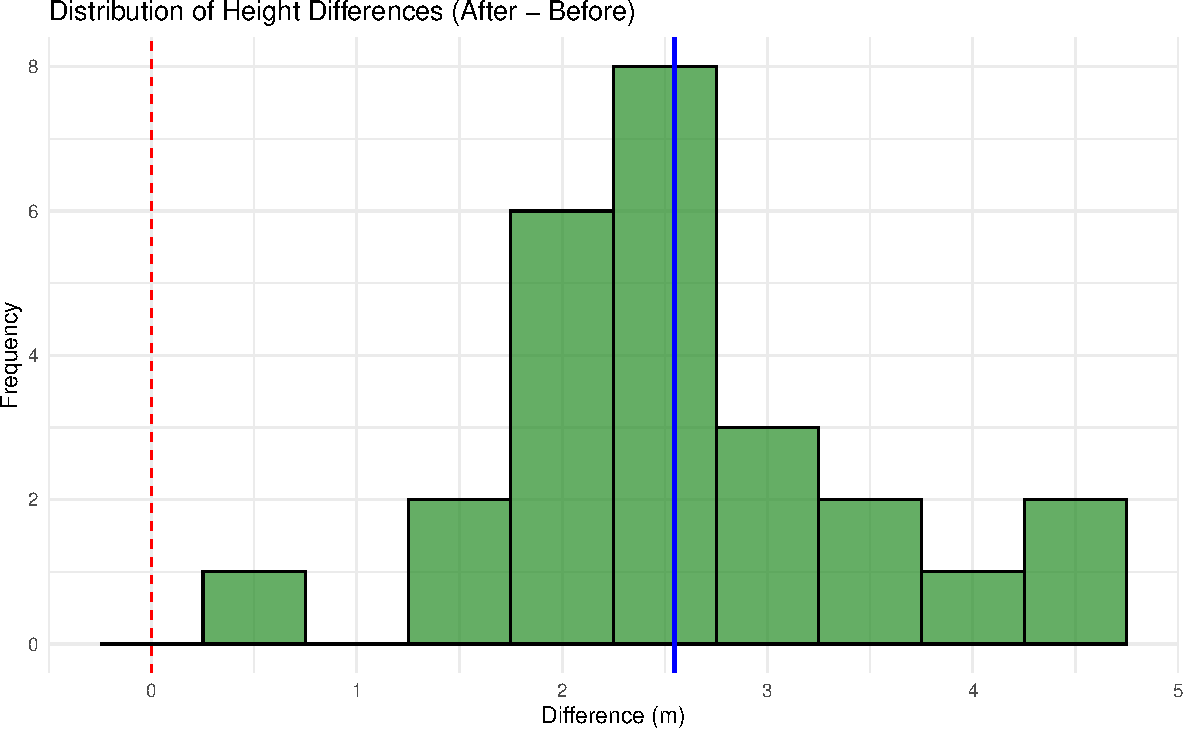
\includegraphics[keepaspectratio]{chapters/07-advanced-visualization_files/figure-pdf/unnamed-chunk-4-2.pdf}}

\subsection{Heatmaps for Community
Data}\label{heatmaps-for-community-data}

Heatmaps are useful for visualizing species-by-site matrices:

\begin{Shaded}
\begin{Highlighting}[]
\CommentTok{\# Create a simulated species{-}by{-}site matrix}
\FunctionTok{set.seed}\NormalTok{(}\DecValTok{123}\NormalTok{)}
\NormalTok{n\_sites }\OtherTok{\textless{}{-}} \DecValTok{10}
\NormalTok{n\_species }\OtherTok{\textless{}{-}} \DecValTok{15}
\NormalTok{community\_matrix }\OtherTok{\textless{}{-}} \FunctionTok{matrix}\NormalTok{(}\FunctionTok{rpois}\NormalTok{(n\_sites }\SpecialCharTok{*}\NormalTok{ n\_species, }\AttributeTok{lambda =} \DecValTok{2}\NormalTok{), }
                          \AttributeTok{nrow =}\NormalTok{ n\_sites, }\AttributeTok{ncol =}\NormalTok{ n\_species)}
\FunctionTok{rownames}\NormalTok{(community\_matrix) }\OtherTok{\textless{}{-}} \FunctionTok{paste0}\NormalTok{(}\StringTok{"Site"}\NormalTok{, }\DecValTok{1}\SpecialCharTok{:}\NormalTok{n\_sites)}
\FunctionTok{colnames}\NormalTok{(community\_matrix) }\OtherTok{\textless{}{-}} \FunctionTok{paste0}\NormalTok{(}\StringTok{"Sp"}\NormalTok{, }\DecValTok{1}\SpecialCharTok{:}\NormalTok{n\_species)}

\CommentTok{\# Convert to long format for ggplot}
\NormalTok{community\_data }\OtherTok{\textless{}{-}} \FunctionTok{as.data.frame}\NormalTok{(}\FunctionTok{as.table}\NormalTok{(community\_matrix))}
\FunctionTok{names}\NormalTok{(community\_data) }\OtherTok{\textless{}{-}} \FunctionTok{c}\NormalTok{(}\StringTok{"Site"}\NormalTok{, }\StringTok{"Species"}\NormalTok{, }\StringTok{"Abundance"}\NormalTok{)}

\CommentTok{\# Create a heatmap}
\FunctionTok{ggplot}\NormalTok{(community\_data, }\FunctionTok{aes}\NormalTok{(}\AttributeTok{x =}\NormalTok{ Species, }\AttributeTok{y =}\NormalTok{ Site, }\AttributeTok{fill =}\NormalTok{ Abundance)) }\SpecialCharTok{+}
  \FunctionTok{geom\_tile}\NormalTok{() }\SpecialCharTok{+}
  \FunctionTok{scale\_fill\_viridis\_c}\NormalTok{() }\SpecialCharTok{+}
  \FunctionTok{labs}\NormalTok{(}\AttributeTok{title =} \StringTok{"Species Abundance by Site"}\NormalTok{,}
       \AttributeTok{x =} \StringTok{"Species"}\NormalTok{,}
       \AttributeTok{y =} \StringTok{"Site"}\NormalTok{,}
       \AttributeTok{fill =} \StringTok{"Abundance"}\NormalTok{) }\SpecialCharTok{+}
  \FunctionTok{theme\_minimal}\NormalTok{() }\SpecialCharTok{+}
  \FunctionTok{theme}\NormalTok{(}\AttributeTok{axis.text.x =} \FunctionTok{element\_text}\NormalTok{(}\AttributeTok{angle =} \DecValTok{45}\NormalTok{, }\AttributeTok{hjust =} \DecValTok{1}\NormalTok{))}
\end{Highlighting}
\end{Shaded}

\pandocbounded{\includegraphics[keepaspectratio]{chapters/07-advanced-visualization_files/figure-pdf/unnamed-chunk-5-1.pdf}}

\subsection{Network Diagrams for Ecological
Interactions}\label{network-diagrams-for-ecological-interactions}

Network diagrams can visualize species interactions:

\begin{Shaded}
\begin{Highlighting}[]
\FunctionTok{library}\NormalTok{(igraph)}
\FunctionTok{library}\NormalTok{(ggraph)}

\CommentTok{\# Create a simulated interaction network}
\FunctionTok{set.seed}\NormalTok{(}\DecValTok{456}\NormalTok{)}
\NormalTok{n\_species }\OtherTok{\textless{}{-}} \DecValTok{10}
\NormalTok{interaction\_matrix }\OtherTok{\textless{}{-}} \FunctionTok{matrix}\NormalTok{(}\FunctionTok{rbinom}\NormalTok{(n\_species}\SpecialCharTok{\^{}}\DecValTok{2}\NormalTok{, }\DecValTok{1}\NormalTok{, }\FloatTok{0.2}\NormalTok{), }
                            \AttributeTok{nrow =}\NormalTok{ n\_species, }\AttributeTok{ncol =}\NormalTok{ n\_species)}
\FunctionTok{diag}\NormalTok{(interaction\_matrix) }\OtherTok{\textless{}{-}} \DecValTok{0}  \CommentTok{\# No self{-}interactions}
\NormalTok{species\_names }\OtherTok{\textless{}{-}} \FunctionTok{paste0}\NormalTok{(}\StringTok{"Species"}\NormalTok{, }\DecValTok{1}\SpecialCharTok{:}\NormalTok{n\_species)}
\FunctionTok{rownames}\NormalTok{(interaction\_matrix) }\OtherTok{\textless{}{-}}\NormalTok{ species\_names}
\FunctionTok{colnames}\NormalTok{(interaction\_matrix) }\OtherTok{\textless{}{-}}\NormalTok{ species\_names}

\CommentTok{\# Convert to igraph object}
\NormalTok{g }\OtherTok{\textless{}{-}} \FunctionTok{graph\_from\_adjacency\_matrix}\NormalTok{(interaction\_matrix, }\AttributeTok{mode =} \StringTok{"directed"}\NormalTok{)}
\FunctionTok{V}\NormalTok{(g)}\SpecialCharTok{$}\NormalTok{type }\OtherTok{\textless{}{-}} \FunctionTok{sample}\NormalTok{(}\FunctionTok{c}\NormalTok{(}\StringTok{"Plant"}\NormalTok{, }\StringTok{"Pollinator"}\NormalTok{, }\StringTok{"Herbivore"}\NormalTok{), n\_species, }\AttributeTok{replace =} \ConstantTok{TRUE}\NormalTok{)}

\CommentTok{\# Create a network diagram}
\FunctionTok{ggraph}\NormalTok{(g, }\AttributeTok{layout =} \StringTok{"fr"}\NormalTok{) }\SpecialCharTok{+}
  \FunctionTok{geom\_edge\_link}\NormalTok{(}\AttributeTok{arrow =} \FunctionTok{arrow}\NormalTok{(}\AttributeTok{length =} \FunctionTok{unit}\NormalTok{(}\DecValTok{2}\NormalTok{, }\StringTok{"mm"}\NormalTok{)), }
                \AttributeTok{end\_cap =} \FunctionTok{circle}\NormalTok{(}\DecValTok{2}\NormalTok{, }\StringTok{"mm"}\NormalTok{),}
                \AttributeTok{color =} \StringTok{"gray50"}\NormalTok{) }\SpecialCharTok{+}
  \FunctionTok{geom\_node\_point}\NormalTok{(}\FunctionTok{aes}\NormalTok{(}\AttributeTok{color =}\NormalTok{ type), }\AttributeTok{size =} \DecValTok{5}\NormalTok{) }\SpecialCharTok{+}
  \FunctionTok{geom\_node\_text}\NormalTok{(}\FunctionTok{aes}\NormalTok{(}\AttributeTok{label =}\NormalTok{ name), }\AttributeTok{repel =} \ConstantTok{TRUE}\NormalTok{) }\SpecialCharTok{+}
  \FunctionTok{scale\_color\_brewer}\NormalTok{(}\AttributeTok{palette =} \StringTok{"Set1"}\NormalTok{) }\SpecialCharTok{+}
  \FunctionTok{labs}\NormalTok{(}\AttributeTok{title =} \StringTok{"Ecological Interaction Network"}\NormalTok{,}
       \AttributeTok{color =} \StringTok{"Species Type"}\NormalTok{) }\SpecialCharTok{+}
  \FunctionTok{theme\_void}\NormalTok{()}
\end{Highlighting}
\end{Shaded}

\pandocbounded{\includegraphics[keepaspectratio]{chapters/07-advanced-visualization_files/figure-pdf/unnamed-chunk-6-1.pdf}}

\section{Visualizing Spatial Data}\label{visualizing-spatial-data}

\subsection{Creating Maps with
ggplot2}\label{creating-maps-with-ggplot2}

Spatial visualization is crucial for ecological data:

\begin{Shaded}
\begin{Highlighting}[]
\FunctionTok{library}\NormalTok{(ggplot2)}
\FunctionTok{library}\NormalTok{(maps)}
\FunctionTok{library}\NormalTok{(knitr)}

\CommentTok{\# Get world map data}
\NormalTok{world }\OtherTok{\textless{}{-}} \FunctionTok{map\_data}\NormalTok{(}\StringTok{"world"}\NormalTok{)}

\CommentTok{\# Create sample species occurrence data}
\FunctionTok{set.seed}\NormalTok{(}\DecValTok{789}\NormalTok{)}
\NormalTok{n\_points }\OtherTok{\textless{}{-}} \DecValTok{100}
\NormalTok{occurrences }\OtherTok{\textless{}{-}} \FunctionTok{data.frame}\NormalTok{(}
  \AttributeTok{species =} \FunctionTok{sample}\NormalTok{(}\FunctionTok{c}\NormalTok{(}\StringTok{"Species A"}\NormalTok{, }\StringTok{"Species B"}\NormalTok{, }\StringTok{"Species C"}\NormalTok{), n\_points, }\AttributeTok{replace =} \ConstantTok{TRUE}\NormalTok{),}
  \AttributeTok{longitude =} \FunctionTok{runif}\NormalTok{(n\_points, }\SpecialCharTok{{-}}\DecValTok{10}\NormalTok{, }\DecValTok{40}\NormalTok{),}
  \AttributeTok{latitude =} \FunctionTok{runif}\NormalTok{(n\_points, }\DecValTok{35}\NormalTok{, }\DecValTok{60}\NormalTok{)}
\NormalTok{)}

\CommentTok{\# Create a map}
\FunctionTok{ggplot}\NormalTok{() }\SpecialCharTok{+}
  \FunctionTok{geom\_polygon}\NormalTok{(}\AttributeTok{data =}\NormalTok{ world, }\FunctionTok{aes}\NormalTok{(}\AttributeTok{x =}\NormalTok{ long, }\AttributeTok{y =}\NormalTok{ lat, }\AttributeTok{group =}\NormalTok{ group), }
               \AttributeTok{fill =} \StringTok{"white"}\NormalTok{, }\AttributeTok{color =} \StringTok{"gray70"}\NormalTok{, }\AttributeTok{size =} \FloatTok{0.2}\NormalTok{) }\SpecialCharTok{+}
  \FunctionTok{geom\_point}\NormalTok{(}\AttributeTok{data =}\NormalTok{ occurrences, }
             \FunctionTok{aes}\NormalTok{(}\AttributeTok{x =}\NormalTok{ longitude, }\AttributeTok{y =}\NormalTok{ latitude, }\AttributeTok{color =}\NormalTok{ species),}
             \AttributeTok{alpha =} \FloatTok{0.7}\NormalTok{, }\AttributeTok{size =} \DecValTok{2}\NormalTok{) }\SpecialCharTok{+}
  \FunctionTok{coord\_fixed}\NormalTok{(}\AttributeTok{xlim =} \FunctionTok{c}\NormalTok{(}\SpecialCharTok{{-}}\DecValTok{10}\NormalTok{, }\DecValTok{40}\NormalTok{), }\AttributeTok{ylim =} \FunctionTok{c}\NormalTok{(}\DecValTok{35}\NormalTok{, }\DecValTok{60}\NormalTok{)) }\SpecialCharTok{+}
  \FunctionTok{scale\_color\_viridis\_d}\NormalTok{(}\AttributeTok{option =} \StringTok{"plasma"}\NormalTok{, }\AttributeTok{end =} \FloatTok{0.8}\NormalTok{) }\SpecialCharTok{+}
  \FunctionTok{labs}\NormalTok{(}\AttributeTok{title =} \StringTok{"Species Distribution Map"}\NormalTok{,}
       \AttributeTok{subtitle =} \StringTok{"Sample occurrences across Europe"}\NormalTok{,}
       \AttributeTok{x =} \StringTok{"Longitude"}\NormalTok{, }\AttributeTok{y =} \StringTok{"Latitude"}\NormalTok{, }\AttributeTok{color =} \StringTok{"Species"}\NormalTok{) }\SpecialCharTok{+}
  \FunctionTok{theme\_minimal}\NormalTok{() }\SpecialCharTok{+}
  \FunctionTok{theme}\NormalTok{(}\AttributeTok{panel.grid.major =} \FunctionTok{element\_line}\NormalTok{(}\AttributeTok{color =} \StringTok{"gray90"}\NormalTok{, }\AttributeTok{size =} \FloatTok{0.2}\NormalTok{))}
\end{Highlighting}
\end{Shaded}

\begin{figure}[H]

{\centering \pandocbounded{\includegraphics[keepaspectratio]{chapters/07-advanced-visualization_files/figure-pdf/spatial-map-1.pdf}}

}

\caption{Distribution of sample species occurrences across Europe. The
map shows the spatial patterns of three different species.}

\end{figure}%

\subsection{Visualizing Raster Data}\label{visualizing-raster-data}

Environmental raster data is common in ecological studies:

\begin{Shaded}
\begin{Highlighting}[]
\FunctionTok{library}\NormalTok{(raster)}
\FunctionTok{library}\NormalTok{(ggplot2)}
\FunctionTok{library}\NormalTok{(viridis)}
\FunctionTok{library}\NormalTok{(maps)}

\CommentTok{\# Create a sample raster}
\NormalTok{r }\OtherTok{\textless{}{-}} \FunctionTok{raster}\NormalTok{(}\AttributeTok{ncol =} \DecValTok{100}\NormalTok{, }\AttributeTok{nrow =} \DecValTok{100}\NormalTok{)}
\FunctionTok{extent}\NormalTok{(r) }\OtherTok{\textless{}{-}} \FunctionTok{c}\NormalTok{(}\SpecialCharTok{{-}}\DecValTok{10}\NormalTok{, }\DecValTok{40}\NormalTok{, }\DecValTok{35}\NormalTok{, }\DecValTok{60}\NormalTok{)  }\CommentTok{\# Same extent as our map}
\FunctionTok{values}\NormalTok{(r) }\OtherTok{\textless{}{-}} \FunctionTok{runif}\NormalTok{(}\FunctionTok{ncell}\NormalTok{(r)) }\SpecialCharTok{*} \DecValTok{10}  \CommentTok{\# Random values}

\CommentTok{\# Convert to data frame for ggplot}
\NormalTok{r\_df }\OtherTok{\textless{}{-}} \FunctionTok{as.data.frame}\NormalTok{(r, }\AttributeTok{xy =} \ConstantTok{TRUE}\NormalTok{)}
\FunctionTok{colnames}\NormalTok{(r\_df) }\OtherTok{\textless{}{-}} \FunctionTok{c}\NormalTok{(}\StringTok{"longitude"}\NormalTok{, }\StringTok{"latitude"}\NormalTok{, }\StringTok{"value"}\NormalTok{)}

\CommentTok{\# Get world map data}
\NormalTok{world }\OtherTok{\textless{}{-}} \FunctionTok{map\_data}\NormalTok{(}\StringTok{"world"}\NormalTok{)}

\CommentTok{\# Create a raster map}
\FunctionTok{ggplot}\NormalTok{() }\SpecialCharTok{+}
  \FunctionTok{geom\_raster}\NormalTok{(}\AttributeTok{data =}\NormalTok{ r\_df, }\FunctionTok{aes}\NormalTok{(}\AttributeTok{x =}\NormalTok{ longitude, }\AttributeTok{y =}\NormalTok{ latitude, }\AttributeTok{fill =}\NormalTok{ value)) }\SpecialCharTok{+}
  \FunctionTok{geom\_polygon}\NormalTok{(}\AttributeTok{data =}\NormalTok{ world, }\FunctionTok{aes}\NormalTok{(}\AttributeTok{x =}\NormalTok{ long, }\AttributeTok{y =}\NormalTok{ lat, }\AttributeTok{group =}\NormalTok{ group), }
               \AttributeTok{fill =} \ConstantTok{NA}\NormalTok{, }\AttributeTok{color =} \StringTok{"gray30"}\NormalTok{, }\AttributeTok{size =} \FloatTok{0.2}\NormalTok{) }\SpecialCharTok{+}
  \FunctionTok{scale\_fill\_viridis\_c}\NormalTok{(}\AttributeTok{option =} \StringTok{"plasma"}\NormalTok{, }\AttributeTok{name =} \StringTok{"Value"}\NormalTok{) }\SpecialCharTok{+}
  \FunctionTok{coord\_fixed}\NormalTok{(}\AttributeTok{xlim =} \FunctionTok{c}\NormalTok{(}\SpecialCharTok{{-}}\DecValTok{10}\NormalTok{, }\DecValTok{40}\NormalTok{), }\AttributeTok{ylim =} \FunctionTok{c}\NormalTok{(}\DecValTok{35}\NormalTok{, }\DecValTok{60}\NormalTok{)) }\SpecialCharTok{+}
  \FunctionTok{labs}\NormalTok{(}\AttributeTok{title =} \StringTok{"Environmental Variable Distribution"}\NormalTok{,}
       \AttributeTok{subtitle =} \StringTok{"Simulated environmental gradient across Europe"}\NormalTok{,}
       \AttributeTok{x =} \StringTok{"Longitude"}\NormalTok{, }\AttributeTok{y =} \StringTok{"Latitude"}\NormalTok{) }\SpecialCharTok{+}
  \FunctionTok{theme\_minimal}\NormalTok{() }\SpecialCharTok{+}
  \FunctionTok{theme}\NormalTok{(}\AttributeTok{panel.grid =} \FunctionTok{element\_blank}\NormalTok{())}
\end{Highlighting}
\end{Shaded}

\begin{figure}[H]

{\centering \pandocbounded{\includegraphics[keepaspectratio]{chapters/07-advanced-visualization_files/figure-pdf/raster-map-1.pdf}}

}

\caption{Environmental variable visualization across Europe. The raster
data shows a simulated environmental gradient overlaid with country
boundaries.}

\end{figure}%

\section{Summary}\label{summary-6}

In this chapter, we've explored advanced visualization techniques in R
that go beyond basic plots. These techniques allow researchers to create
more informative, interactive, and publication-quality visualizations
for ecological and forestry data.

Key points covered include:

\begin{itemize}
\tightlist
\item
  Creating complex multi-panel visualizations
\item
  Developing interactive plots for exploration
\item
  Designing effective spatial visualizations
\item
  Implementing animation for temporal data
\item
  Customizing visualizations for publication
\end{itemize}

As you continue to develop your data visualization skills, remember that
effective visualization is both an art and a science. The goal is not
just to make visually appealing graphics, but to create visualizations
that accurately and clearly communicate your findings to your audience.

\section{Exercises}\label{exercises-6}

\begin{enumerate}
\def\labelenumi{\arabic{enumi}.}
\tightlist
\item
  Create a faceted plot showing the relationship between two variables
  across different categories in one of the datasets.
\item
  Develop an interactive plot that allows users to explore relationships
  in ecological data.
\item
  Create a custom theme for ggplot2 that matches the style guidelines of
  a scientific journal in your field.
\item
  Design a spatial visualization showing the distribution of a species
  or environmental variable.
\item
  Create an animated plot showing changes in an ecological variable over
  time.
\end{enumerate}

\part{Advanced Topics}

\chapter{Regression Analysis}\label{regression-analysis-1}

\section{Introduction}\label{introduction-6}

Regression analysis is a powerful statistical technique used to model
the relationship between a dependent variable and one or more
independent variables. In natural sciences research, regression models
help us understand how environmental factors influence biological
processes, predict future conditions, and test hypotheses about causal
relationships.

\section{Simple Linear Regression}\label{simple-linear-regression}

Simple linear regression models the relationship between a dependent
variable and a single independent variable.

\subsection{The Linear Model}\label{the-linear-model}

The simple linear regression model is represented by the equation:

\[Y = \beta_0 + \beta_1X + \varepsilon\]

Where: - \(Y\) is the dependent variable - \(X\) is the independent
variable - \(\beta_0\) is the intercept - \(\beta_1\) is the slope -
\(\varepsilon\) is the error term

\subsection{Example: Crop Yield Trends Over
Time}\label{example-crop-yield-trends-over-time}

Let's explore the relationship between time (years) and wheat yields
using our agricultural dataset:

\begin{Shaded}
\begin{Highlighting}[]
\CommentTok{\# Load necessary libraries}
\FunctionTok{library}\NormalTok{(tidyverse)}

\CommentTok{\# Load the crop yield dataset}
\NormalTok{crop\_yields }\OtherTok{\textless{}{-}} \FunctionTok{read\_csv}\NormalTok{(}\StringTok{"../data/agriculture/crop\_yields.csv"}\NormalTok{)}

\CommentTok{\# Filter data for a specific country (United States) and select relevant columns}
\NormalTok{us\_wheat }\OtherTok{\textless{}{-}}\NormalTok{ crop\_yields }\SpecialCharTok{\%\textgreater{}\%}
  \FunctionTok{filter}\NormalTok{(Entity }\SpecialCharTok{==} \StringTok{"United States"}\NormalTok{, }\SpecialCharTok{!}\FunctionTok{is.na}\NormalTok{(}\StringTok{\textasciigrave{}}\AttributeTok{Wheat (tonnes per hectare)}\StringTok{\textasciigrave{}}\NormalTok{)) }\SpecialCharTok{\%\textgreater{}\%}
  \FunctionTok{select}\NormalTok{(Year, }\StringTok{\textasciigrave{}}\AttributeTok{Wheat (tonnes per hectare)}\StringTok{\textasciigrave{}}\NormalTok{)}

\CommentTok{\# Visualize the relationship}
\FunctionTok{ggplot}\NormalTok{(us\_wheat, }\FunctionTok{aes}\NormalTok{(}\AttributeTok{x =}\NormalTok{ Year, }\AttributeTok{y =} \StringTok{\textasciigrave{}}\AttributeTok{Wheat (tonnes per hectare)}\StringTok{\textasciigrave{}}\NormalTok{)) }\SpecialCharTok{+}
  \FunctionTok{geom\_point}\NormalTok{(}\AttributeTok{size =} \DecValTok{3}\NormalTok{, }\AttributeTok{alpha =} \FloatTok{0.7}\NormalTok{) }\SpecialCharTok{+}
  \FunctionTok{labs}\NormalTok{(}\AttributeTok{title =} \StringTok{"Wheat Yields in the United States (1961{-}present)"}\NormalTok{,}
       \AttributeTok{x =} \StringTok{"Year"}\NormalTok{,}
       \AttributeTok{y =} \StringTok{"Wheat Yield (tonnes per hectare)"}\NormalTok{) }\SpecialCharTok{+}
  \FunctionTok{theme\_minimal}\NormalTok{()}
\end{Highlighting}
\end{Shaded}

\pandocbounded{\includegraphics[keepaspectratio]{chapters/08-regression_files/figure-pdf/unnamed-chunk-1-1.pdf}}

\begin{Shaded}
\begin{Highlighting}[]
\CommentTok{\# Fit a simple linear regression model}
\NormalTok{model }\OtherTok{\textless{}{-}} \FunctionTok{lm}\NormalTok{(}\StringTok{\textasciigrave{}}\AttributeTok{Wheat (tonnes per hectare)}\StringTok{\textasciigrave{}} \SpecialCharTok{\textasciitilde{}}\NormalTok{ Year, }\AttributeTok{data =}\NormalTok{ us\_wheat)}

\CommentTok{\# Display model summary}
\FunctionTok{summary}\NormalTok{(model)}
\end{Highlighting}
\end{Shaded}

\begin{verbatim}

Call:
lm(formula = `Wheat (tonnes per hectare)` ~ Year, data = us_wheat)

Residuals:
     Min       1Q   Median       3Q      Max 
-0.43042 -0.09139 -0.00340  0.11184  0.39526 

Coefficients:
              Estimate Std. Error t value Pr(>|t|)    
(Intercept) -48.465987   2.571017  -18.85   <2e-16 ***
Year          0.025601   0.001292   19.81   <2e-16 ***
---
Signif. codes:  0 '***' 0.001 '**' 0.01 '*' 0.05 '.' 0.1 ' ' 1

Residual standard error: 0.1648 on 56 degrees of freedom
Multiple R-squared:  0.8751,    Adjusted R-squared:  0.8729 
F-statistic: 392.5 on 1 and 56 DF,  p-value: < 2.2e-16
\end{verbatim}

\begin{Shaded}
\begin{Highlighting}[]
\CommentTok{\# Add the regression line to the plot}
\FunctionTok{ggplot}\NormalTok{(us\_wheat, }\FunctionTok{aes}\NormalTok{(}\AttributeTok{x =}\NormalTok{ Year, }\AttributeTok{y =} \StringTok{\textasciigrave{}}\AttributeTok{Wheat (tonnes per hectare)}\StringTok{\textasciigrave{}}\NormalTok{)) }\SpecialCharTok{+}
  \FunctionTok{geom\_point}\NormalTok{(}\AttributeTok{size =} \DecValTok{3}\NormalTok{, }\AttributeTok{alpha =} \FloatTok{0.7}\NormalTok{) }\SpecialCharTok{+}
  \FunctionTok{geom\_smooth}\NormalTok{(}\AttributeTok{method =} \StringTok{"lm"}\NormalTok{, }\AttributeTok{color =} \StringTok{"blue"}\NormalTok{) }\SpecialCharTok{+}
  \FunctionTok{labs}\NormalTok{(}\AttributeTok{title =} \StringTok{"Simple Linear Regression: Wheat Yield vs. Year"}\NormalTok{,}
       \AttributeTok{x =} \StringTok{"Year"}\NormalTok{,}
       \AttributeTok{y =} \StringTok{"Wheat Yield (tonnes per hectare)"}\NormalTok{) }\SpecialCharTok{+}
  \FunctionTok{theme\_minimal}\NormalTok{()}
\end{Highlighting}
\end{Shaded}

\pandocbounded{\includegraphics[keepaspectratio]{chapters/08-regression_files/figure-pdf/unnamed-chunk-1-2.pdf}}

\subsection{Interpreting the Model}\label{interpreting-the-model}

The key components to interpret in a simple linear regression model are:

\begin{enumerate}
\def\labelenumi{\arabic{enumi}.}
\tightlist
\item
  \textbf{Intercept (\(\beta_0\))}: The expected value of Y when X = 0
\item
  \textbf{Slope (\(\beta_1\))}: The expected change in Y for a one-unit
  increase in X
\item
  \textbf{R-squared}: The proportion of variance in Y explained by X
\item
  \textbf{p-value}: The statistical significance of the relationship
\end{enumerate}

\begin{Shaded}
\begin{Highlighting}[]
\CommentTok{\# Extract key model parameters}
\NormalTok{intercept }\OtherTok{\textless{}{-}} \FunctionTok{coef}\NormalTok{(model)[}\DecValTok{1}\NormalTok{]}
\NormalTok{slope }\OtherTok{\textless{}{-}} \FunctionTok{coef}\NormalTok{(model)[}\DecValTok{2}\NormalTok{]}
\NormalTok{r\_squared }\OtherTok{\textless{}{-}} \FunctionTok{summary}\NormalTok{(model)}\SpecialCharTok{$}\NormalTok{r.squared}
\NormalTok{p\_value }\OtherTok{\textless{}{-}} \FunctionTok{summary}\NormalTok{(model)}\SpecialCharTok{$}\NormalTok{coefficients[}\DecValTok{2}\NormalTok{, }\DecValTok{4}\NormalTok{]}

\CommentTok{\# Create a table of results}
\NormalTok{results }\OtherTok{\textless{}{-}} \FunctionTok{data.frame}\NormalTok{(}
  \AttributeTok{Parameter =} \FunctionTok{c}\NormalTok{(}\StringTok{"Intercept"}\NormalTok{, }\StringTok{"Slope"}\NormalTok{, }\StringTok{"R{-}squared"}\NormalTok{, }\StringTok{"p{-}value"}\NormalTok{),}
  \AttributeTok{Value =} \FunctionTok{c}\NormalTok{(intercept, slope, r\_squared, p\_value)}
\NormalTok{)}

\CommentTok{\# Display the results}
\NormalTok{knitr}\SpecialCharTok{::}\FunctionTok{kable}\NormalTok{(results, }\AttributeTok{digits =} \DecValTok{4}\NormalTok{)}
\end{Highlighting}
\end{Shaded}

\begin{longtable}[]{@{}lr@{}}
\toprule\noalign{}
Parameter & Value \\
\midrule\noalign{}
\endhead
\bottomrule\noalign{}
\endlastfoot
Intercept & -48.4660 \\
Slope & 0.0256 \\
R-squared & 0.8751 \\
p-value & 0.0000 \\
\end{longtable}

In this example, the slope represents the average annual increase in
wheat yield (tonnes/hectare) in the United States. The R-squared value
indicates what percentage of the variation in wheat yields can be
explained by the year. The p-value tells us whether this relationship is
statistically significant.

\subsection{Checking Model
Assumptions}\label{checking-model-assumptions}

Linear regression relies on several key assumptions:

\begin{enumerate}
\def\labelenumi{\arabic{enumi}.}
\tightlist
\item
  \textbf{Linearity}: The relationship between X and Y is linear
\item
  \textbf{Independence}: Observations are independent of each other
\item
  \textbf{Homoscedasticity}: Constant variance of residuals
\item
  \textbf{Normality}: Residuals are normally distributed
\end{enumerate}

\begin{Shaded}
\begin{Highlighting}[]
\CommentTok{\# Diagnostic plots}
\FunctionTok{par}\NormalTok{(}\AttributeTok{mfrow =} \FunctionTok{c}\NormalTok{(}\DecValTok{2}\NormalTok{, }\DecValTok{2}\NormalTok{))}
\FunctionTok{plot}\NormalTok{(model)}
\end{Highlighting}
\end{Shaded}

\pandocbounded{\includegraphics[keepaspectratio]{chapters/08-regression_files/figure-pdf/unnamed-chunk-3-1.pdf}}

\begin{Shaded}
\begin{Highlighting}[]
\CommentTok{\# Check normality of residuals with a formal test}
\FunctionTok{shapiro.test}\NormalTok{(}\FunctionTok{residuals}\NormalTok{(model))}
\end{Highlighting}
\end{Shaded}

\begin{verbatim}

    Shapiro-Wilk normality test

data:  residuals(model)
W = 0.99033, p-value = 0.9252
\end{verbatim}

\begin{Shaded}
\begin{Highlighting}[]
\CommentTok{\# Check homoscedasticity with a formal test}
\ControlFlowTok{if}\NormalTok{(}\FunctionTok{requireNamespace}\NormalTok{(}\StringTok{"car"}\NormalTok{, }\AttributeTok{quietly =} \ConstantTok{TRUE}\NormalTok{)) \{}
  \FunctionTok{library}\NormalTok{(car)}
  \FunctionTok{ncvTest}\NormalTok{(model)}
\NormalTok{\} }\ControlFlowTok{else}\NormalTok{ \{}
  \FunctionTok{message}\NormalTok{(}\StringTok{"The \textquotesingle{}car\textquotesingle{} package is not installed. Install it with install.packages(\textquotesingle{}car\textquotesingle{}) to run the non{-}constant variance test."}\NormalTok{)}
\NormalTok{\}}
\end{Highlighting}
\end{Shaded}

\begin{verbatim}
Non-constant Variance Score Test 
Variance formula: ~ fitted.values 
Chisquare = 1.323418, Df = 1, p = 0.24998
\end{verbatim}

\section{Multiple Linear Regression}\label{multiple-linear-regression}

Multiple linear regression extends the simple linear model to include
multiple independent variables.

\subsection{The Multiple Regression
Model}\label{the-multiple-regression-model}

The multiple regression model is represented by the equation:

\[Y = \beta_0 + \beta_1X_1 + \beta_2X_2 + ... + \beta_pX_p + \varepsilon\]

Where: - \(Y\) is the dependent variable - \(X_1, X_2, ..., X_p\) are
the independent variables - \(\beta_0, \beta_1, \beta_2, ..., \beta_p\)
are the coefficients - \(\varepsilon\) is the error term

\subsection{Example: Factors Affecting Crop
Yields}\label{example-factors-affecting-crop-yields}

Let's model wheat yield as a function of multiple crop yields, which
might indicate similar agricultural conditions:

\begin{Shaded}
\begin{Highlighting}[]
\CommentTok{\# Prepare data for multiple regression}
\NormalTok{multi\_crop\_data }\OtherTok{\textless{}{-}}\NormalTok{ crop\_yields }\SpecialCharTok{\%\textgreater{}\%}
  \FunctionTok{filter}\NormalTok{(}\SpecialCharTok{!}\FunctionTok{is.na}\NormalTok{(}\StringTok{\textasciigrave{}}\AttributeTok{Wheat (tonnes per hectare)}\StringTok{\textasciigrave{}}\NormalTok{) }\SpecialCharTok{\&} \SpecialCharTok{!}\FunctionTok{is.na}\NormalTok{(}\StringTok{\textasciigrave{}}\AttributeTok{Rice (tonnes per hectare)}\StringTok{\textasciigrave{}}\NormalTok{) }\SpecialCharTok{\&} \SpecialCharTok{!}\FunctionTok{is.na}\NormalTok{(}\StringTok{\textasciigrave{}}\AttributeTok{Maize (tonnes per hectare)}\StringTok{\textasciigrave{}}\NormalTok{)) }\SpecialCharTok{\%\textgreater{}\%}
  \FunctionTok{select}\NormalTok{(Entity, Year, }\StringTok{\textasciigrave{}}\AttributeTok{Wheat (tonnes per hectare)}\StringTok{\textasciigrave{}}\NormalTok{, }\StringTok{\textasciigrave{}}\AttributeTok{Rice (tonnes per hectare)}\StringTok{\textasciigrave{}}\NormalTok{, }\StringTok{\textasciigrave{}}\AttributeTok{Maize (tonnes per hectare)}\StringTok{\textasciigrave{}}\NormalTok{)}

\CommentTok{\# View the first few rows}
\FunctionTok{head}\NormalTok{(multi\_crop\_data)}
\end{Highlighting}
\end{Shaded}

\begin{verbatim}
# A tibble: 6 x 5
  Entity       Year `Wheat (tonnes per hectare)` `Rice (tonnes per hectare)`
  <chr>       <dbl>                        <dbl>                       <dbl>
1 Afghanistan  1961                        1.02                         1.52
2 Afghanistan  1962                        0.974                        1.52
3 Afghanistan  1963                        0.832                        1.52
4 Afghanistan  1964                        0.951                        1.73
5 Afghanistan  1965                        0.972                        1.73
6 Afghanistan  1966                        0.867                        1.52
# i 1 more variable: `Maize (tonnes per hectare)` <dbl>
\end{verbatim}

\begin{Shaded}
\begin{Highlighting}[]
\CommentTok{\# Fit a multiple regression model}
\NormalTok{multi\_model }\OtherTok{\textless{}{-}} \FunctionTok{lm}\NormalTok{(}\StringTok{\textasciigrave{}}\AttributeTok{Wheat (tonnes per hectare)}\StringTok{\textasciigrave{}} \SpecialCharTok{\textasciitilde{}} \StringTok{\textasciigrave{}}\AttributeTok{Rice (tonnes per hectare)}\StringTok{\textasciigrave{}} \SpecialCharTok{+} \StringTok{\textasciigrave{}}\AttributeTok{Maize (tonnes per hectare)}\StringTok{\textasciigrave{}} \SpecialCharTok{+}\NormalTok{ Year, }\AttributeTok{data =}\NormalTok{ multi\_crop\_data)}

\CommentTok{\# Display model summary}
\FunctionTok{summary}\NormalTok{(multi\_model)}
\end{Highlighting}
\end{Shaded}

\begin{verbatim}

Call:
lm(formula = `Wheat (tonnes per hectare)` ~ `Rice (tonnes per hectare)` + 
    `Maize (tonnes per hectare)` + Year, data = multi_crop_data)

Residuals:
    Min      1Q  Median      3Q     Max 
-2.7029 -0.6135 -0.2079  0.3877  7.8709 

Coefficients:
                               Estimate Std. Error t value Pr(>|t|)    
(Intercept)                  -2.161e+01  1.776e+00 -12.171   <2e-16 ***
`Rice (tonnes per hectare)`  -5.426e-03  9.720e-03  -0.558    0.577    
`Maize (tonnes per hectare)`  2.790e-01  8.512e-03  32.776   <2e-16 ***
Year                          1.148e-02  8.965e-04  12.810   <2e-16 ***
---
Signif. codes:  0 '***' 0.001 '**' 0.01 '*' 0.05 '.' 0.1 ' ' 1

Residual standard error: 1.025 on 5722 degrees of freedom
Multiple R-squared:  0.3411,    Adjusted R-squared:  0.3407 
F-statistic: 987.2 on 3 and 5722 DF,  p-value: < 2.2e-16
\end{verbatim}

\subsection{Visualizing Multiple
Regression}\label{visualizing-multiple-regression}

Visualizing multiple regression models is challenging due to the
multidimensional nature of the data. Here are some approaches:

\begin{Shaded}
\begin{Highlighting}[]
\CommentTok{\# Partial residual plots}
\ControlFlowTok{if}\NormalTok{(}\FunctionTok{requireNamespace}\NormalTok{(}\StringTok{"car"}\NormalTok{, }\AttributeTok{quietly =} \ConstantTok{TRUE}\NormalTok{)) \{}
  \FunctionTok{library}\NormalTok{(car)}
  \CommentTok{\# Create a model with simpler variable names to avoid issues with crPlots}
\NormalTok{  renamed\_data }\OtherTok{\textless{}{-}}\NormalTok{ multi\_crop\_data }\SpecialCharTok{\%\textgreater{}\%}
    \FunctionTok{rename}\NormalTok{(}\AttributeTok{Wheat =} \StringTok{\textasciigrave{}}\AttributeTok{Wheat (tonnes per hectare)}\StringTok{\textasciigrave{}}\NormalTok{,}
           \AttributeTok{Rice =} \StringTok{\textasciigrave{}}\AttributeTok{Rice (tonnes per hectare)}\StringTok{\textasciigrave{}}\NormalTok{,}
           \AttributeTok{Maize =} \StringTok{\textasciigrave{}}\AttributeTok{Maize (tonnes per hectare)}\StringTok{\textasciigrave{}}\NormalTok{)}
  
\NormalTok{  simple\_model }\OtherTok{\textless{}{-}} \FunctionTok{lm}\NormalTok{(Wheat }\SpecialCharTok{\textasciitilde{}}\NormalTok{ Rice }\SpecialCharTok{+}\NormalTok{ Maize }\SpecialCharTok{+}\NormalTok{ Year, }\AttributeTok{data =}\NormalTok{ renamed\_data)}
  \FunctionTok{crPlots}\NormalTok{(simple\_model)}
\NormalTok{\} }\ControlFlowTok{else}\NormalTok{ \{}
  \CommentTok{\# Alternative: create individual scatter plots}
  \FunctionTok{par}\NormalTok{(}\AttributeTok{mfrow =} \FunctionTok{c}\NormalTok{(}\DecValTok{1}\NormalTok{, }\DecValTok{3}\NormalTok{))}
  \FunctionTok{plot}\NormalTok{(multi\_crop\_data}\SpecialCharTok{$}\StringTok{\textasciigrave{}}\AttributeTok{Rice (tonnes per hectare)}\StringTok{\textasciigrave{}}\NormalTok{, multi\_crop\_data}\SpecialCharTok{$}\StringTok{\textasciigrave{}}\AttributeTok{Wheat (tonnes per hectare)}\StringTok{\textasciigrave{}}\NormalTok{, }
       \AttributeTok{xlab =} \StringTok{"Rice Yield"}\NormalTok{, }\AttributeTok{ylab =} \StringTok{"Wheat Yield"}\NormalTok{,}
       \AttributeTok{main =} \StringTok{"Wheat vs. Rice"}\NormalTok{)}
  \FunctionTok{plot}\NormalTok{(multi\_crop\_data}\SpecialCharTok{$}\StringTok{\textasciigrave{}}\AttributeTok{Maize (tonnes per hectare)}\StringTok{\textasciigrave{}}\NormalTok{, multi\_crop\_data}\SpecialCharTok{$}\StringTok{\textasciigrave{}}\AttributeTok{Wheat (tonnes per hectare)}\StringTok{\textasciigrave{}}\NormalTok{, }
       \AttributeTok{xlab =} \StringTok{"Maize Yield"}\NormalTok{, }\AttributeTok{ylab =} \StringTok{"Wheat Yield"}\NormalTok{,}
       \AttributeTok{main =} \StringTok{"Wheat vs. Maize"}\NormalTok{)}
  \FunctionTok{plot}\NormalTok{(multi\_crop\_data}\SpecialCharTok{$}\NormalTok{Year, multi\_crop\_data}\SpecialCharTok{$}\StringTok{\textasciigrave{}}\AttributeTok{Wheat (tonnes per hectare)}\StringTok{\textasciigrave{}}\NormalTok{, }
       \AttributeTok{xlab =} \StringTok{"Year"}\NormalTok{, }\AttributeTok{ylab =} \StringTok{"Wheat Yield"}\NormalTok{,}
       \AttributeTok{main =} \StringTok{"Wheat vs. Year"}\NormalTok{)}
\NormalTok{\}}
\end{Highlighting}
\end{Shaded}

\pandocbounded{\includegraphics[keepaspectratio]{chapters/08-regression_files/figure-pdf/unnamed-chunk-5-1.pdf}}

\begin{Shaded}
\begin{Highlighting}[]
\CommentTok{\# 3D visualization (for a subset of variables)}
\FunctionTok{library}\NormalTok{(knitr)}
\ControlFlowTok{if}\NormalTok{(knitr}\SpecialCharTok{::}\FunctionTok{is\_html\_output}\NormalTok{() }\SpecialCharTok{\&\&} \FunctionTok{requireNamespace}\NormalTok{(}\StringTok{"plotly"}\NormalTok{, }\AttributeTok{quietly =} \ConstantTok{TRUE}\NormalTok{)) \{}
  \CommentTok{\# For HTML output, use the interactive plotly version}
  \FunctionTok{library}\NormalTok{(plotly)}
  \FunctionTok{plot\_ly}\NormalTok{(multi\_crop\_data, }
          \AttributeTok{x =} \SpecialCharTok{\textasciitilde{}}\StringTok{\textasciigrave{}}\AttributeTok{Rice (tonnes per hectare)}\StringTok{\textasciigrave{}}\NormalTok{, }
          \AttributeTok{y =} \SpecialCharTok{\textasciitilde{}}\StringTok{\textasciigrave{}}\AttributeTok{Maize (tonnes per hectare)}\StringTok{\textasciigrave{}}\NormalTok{, }
          \AttributeTok{z =} \SpecialCharTok{\textasciitilde{}}\StringTok{\textasciigrave{}}\AttributeTok{Wheat (tonnes per hectare)}\StringTok{\textasciigrave{}}\NormalTok{,}
          \AttributeTok{type =} \StringTok{"scatter3d"}\NormalTok{, }\AttributeTok{mode =} \StringTok{"markers"}\NormalTok{,}
          \AttributeTok{marker =} \FunctionTok{list}\NormalTok{(}\AttributeTok{size =} \DecValTok{5}\NormalTok{, }\AttributeTok{color =} \SpecialCharTok{\textasciitilde{}}\StringTok{\textasciigrave{}}\AttributeTok{Wheat (tonnes per hectare)}\StringTok{\textasciigrave{}}\NormalTok{, }
                        \AttributeTok{colorscale =} \StringTok{"Viridis"}\NormalTok{)) }\SpecialCharTok{\%\textgreater{}\%}
    \FunctionTok{layout}\NormalTok{(}\AttributeTok{title =} \StringTok{"3D Relationship Between Crop Yields"}\NormalTok{,}
           \AttributeTok{scene =} \FunctionTok{list}\NormalTok{(}
             \AttributeTok{xaxis =} \FunctionTok{list}\NormalTok{(}\AttributeTok{title =} \StringTok{"Rice Yield (tonnes/ha)"}\NormalTok{),}
             \AttributeTok{yaxis =} \FunctionTok{list}\NormalTok{(}\AttributeTok{title =} \StringTok{"Maize Yield (tonnes/ha)"}\NormalTok{),}
             \AttributeTok{zaxis =} \FunctionTok{list}\NormalTok{(}\AttributeTok{title =} \StringTok{"Wheat Yield (tonnes/ha)"}\NormalTok{)))}
\NormalTok{\} }\ControlFlowTok{else}\NormalTok{ \{}
  \CommentTok{\# For PDF output, use a static 3D scatter plot with ggplot2}
  \FunctionTok{library}\NormalTok{(ggplot2)}
  
  \CommentTok{\# Create a 2D plot with color as the third dimension}
  \FunctionTok{ggplot}\NormalTok{(multi\_crop\_data, }
         \FunctionTok{aes}\NormalTok{(}\AttributeTok{x =} \StringTok{\textasciigrave{}}\AttributeTok{Rice (tonnes per hectare)}\StringTok{\textasciigrave{}}\NormalTok{, }
             \AttributeTok{y =} \StringTok{\textasciigrave{}}\AttributeTok{Maize (tonnes per hectare)}\StringTok{\textasciigrave{}}\NormalTok{, }
             \AttributeTok{color =} \StringTok{\textasciigrave{}}\AttributeTok{Wheat (tonnes per hectare)}\StringTok{\textasciigrave{}}\NormalTok{)) }\SpecialCharTok{+}
    \FunctionTok{geom\_point}\NormalTok{(}\AttributeTok{size =} \DecValTok{3}\NormalTok{, }\AttributeTok{alpha =} \FloatTok{0.7}\NormalTok{) }\SpecialCharTok{+}
    \FunctionTok{scale\_color\_viridis\_c}\NormalTok{(}\AttributeTok{option =} \StringTok{"viridis"}\NormalTok{, }\AttributeTok{name =} \StringTok{"Wheat Yield}\SpecialCharTok{\textbackslash{}n}\StringTok{(tonnes/ha)"}\NormalTok{) }\SpecialCharTok{+}
    \FunctionTok{labs}\NormalTok{(}\AttributeTok{title =} \StringTok{"3D Relationship Between Crop Yields"}\NormalTok{,}
         \AttributeTok{subtitle =} \StringTok{"Wheat yield shown as color (interactive 3D version in HTML)"}\NormalTok{,}
         \AttributeTok{x =} \StringTok{"Rice Yield (tonnes/ha)"}\NormalTok{,}
         \AttributeTok{y =} \StringTok{"Maize Yield (tonnes/ha)"}\NormalTok{) }\SpecialCharTok{+}
    \FunctionTok{theme\_minimal}\NormalTok{() }\SpecialCharTok{+}
    \FunctionTok{theme}\NormalTok{(}\AttributeTok{legend.position =} \StringTok{"right"}\NormalTok{)}
\NormalTok{\}}
\end{Highlighting}
\end{Shaded}

\pandocbounded{\includegraphics[keepaspectratio]{chapters/08-regression_files/figure-pdf/unnamed-chunk-5-2.pdf}}

\subsection{Variable Selection}\label{variable-selection}

When working with multiple predictors, it's essential to select the most
relevant variables:

\begin{Shaded}
\begin{Highlighting}[]
\CommentTok{\# Stepwise variable selection}
\ControlFlowTok{if}\NormalTok{(}\FunctionTok{requireNamespace}\NormalTok{(}\StringTok{"MASS"}\NormalTok{, }\AttributeTok{quietly =} \ConstantTok{TRUE}\NormalTok{)) \{}
  \FunctionTok{library}\NormalTok{(MASS)}
\NormalTok{  step\_model }\OtherTok{\textless{}{-}} \FunctionTok{stepAIC}\NormalTok{(multi\_model, }\AttributeTok{direction =} \StringTok{"both"}\NormalTok{)}
  \FunctionTok{summary}\NormalTok{(step\_model)}
\NormalTok{\} }\ControlFlowTok{else}\NormalTok{ \{}
  \FunctionTok{message}\NormalTok{(}\StringTok{"The \textquotesingle{}MASS\textquotesingle{} package is not installed. Install it with install.packages(\textquotesingle{}MASS\textquotesingle{}) to perform stepwise variable selection."}\NormalTok{)}
\NormalTok{\}}
\end{Highlighting}
\end{Shaded}

\begin{verbatim}
Start:  AIC=292.2
`Wheat (tonnes per hectare)` ~ `Rice (tonnes per hectare)` + 
    `Maize (tonnes per hectare)` + Year

                               Df Sum of Sq    RSS     AIC
- `Rice (tonnes per hectare)`   1      0.33 6017.7  290.51
<none>                                      6017.4  292.20
- Year                          1    172.58 6189.9  452.11
- `Maize (tonnes per hectare)`  1   1129.71 7147.1 1275.38

Step:  AIC=290.51
`Wheat (tonnes per hectare)` ~ `Maize (tonnes per hectare)` + 
    Year

                               Df Sum of Sq    RSS     AIC
<none>                                      6017.7  290.51
+ `Rice (tonnes per hectare)`   1      0.33 6017.4  292.20
- Year                          1    172.33 6190.0  450.18
- `Maize (tonnes per hectare)`  1   1930.18 7947.9 1881.48
\end{verbatim}

\begin{verbatim}

Call:
lm(formula = `Wheat (tonnes per hectare)` ~ `Maize (tonnes per hectare)` + 
    Year, data = multi_crop_data)

Residuals:
    Min      1Q  Median      3Q     Max 
-2.6986 -0.6123 -0.2065  0.3857  7.8812 

Coefficients:
                               Estimate Std. Error t value Pr(>|t|)    
(Intercept)                  -2.156e+01  1.773e+00  -12.16   <2e-16 ***
`Maize (tonnes per hectare)`  2.759e-01  6.439e-03   42.84   <2e-16 ***
Year                          1.145e-02  8.946e-04   12.80   <2e-16 ***
---
Signif. codes:  0 '***' 0.001 '**' 0.01 '*' 0.05 '.' 0.1 ' ' 1

Residual standard error: 1.025 on 5723 degrees of freedom
Multiple R-squared:  0.341, Adjusted R-squared:  0.3408 
F-statistic:  1481 on 2 and 5723 DF,  p-value: < 2.2e-16
\end{verbatim}

\begin{Shaded}
\begin{Highlighting}[]
\CommentTok{\# Variance Inflation Factor (VIF) to check for multicollinearity}
\ControlFlowTok{if}\NormalTok{(}\FunctionTok{requireNamespace}\NormalTok{(}\StringTok{"car"}\NormalTok{, }\AttributeTok{quietly =} \ConstantTok{TRUE}\NormalTok{)) \{}
  \CommentTok{\# Use the renamed data and simple model from earlier}
  \FunctionTok{vif}\NormalTok{(simple\_model)}
\NormalTok{\} }\ControlFlowTok{else}\NormalTok{ \{}
  \FunctionTok{message}\NormalTok{(}\StringTok{"The \textquotesingle{}car\textquotesingle{} package is not installed. Install it with install.packages(\textquotesingle{}car\textquotesingle{}) to calculate VIF values."}\NormalTok{)}
  
  \CommentTok{\# Alternative: correlation matrix}
\NormalTok{  cor\_matrix }\OtherTok{\textless{}{-}} \FunctionTok{cor}\NormalTok{(multi\_crop\_data[, }\FunctionTok{c}\NormalTok{(}\StringTok{"Rice (tonnes per hectare)"}\NormalTok{, }\StringTok{"Maize (tonnes per hectare)"}\NormalTok{, }\StringTok{"Year"}\NormalTok{)], }\AttributeTok{use =} \StringTok{"complete.obs"}\NormalTok{)}
  \FunctionTok{print}\NormalTok{(}\StringTok{"Correlation matrix of predictors:"}\NormalTok{)}
  \FunctionTok{print}\NormalTok{(cor\_matrix)}
\NormalTok{\}}
\end{Highlighting}
\end{Shaded}

\begin{verbatim}
    Rice    Maize     Year 
1.963261 2.108941 1.212106 
\end{verbatim}

\section{Polynomial Regression}\label{polynomial-regression}

Polynomial regression allows modeling of nonlinear relationships by
including polynomial terms.

\subsection{Example: Nonlinear Crop Yield
Trends}\label{example-nonlinear-crop-yield-trends}

Let's explore whether the relationship between time and wheat yields
might be nonlinear:

\begin{Shaded}
\begin{Highlighting}[]
\CommentTok{\# Create a dataset for polynomial regression}
\NormalTok{us\_wheat}\SpecialCharTok{$}\NormalTok{Year\_centered }\OtherTok{\textless{}{-}}\NormalTok{ us\_wheat}\SpecialCharTok{$}\NormalTok{Year }\SpecialCharTok{{-}} \FunctionTok{mean}\NormalTok{(us\_wheat}\SpecialCharTok{$}\NormalTok{Year)  }\CommentTok{\# Center year to reduce multicollinearity}

\CommentTok{\# Fit polynomial models of different degrees}
\NormalTok{poly1 }\OtherTok{\textless{}{-}} \FunctionTok{lm}\NormalTok{(}\StringTok{\textasciigrave{}}\AttributeTok{Wheat (tonnes per hectare)}\StringTok{\textasciigrave{}} \SpecialCharTok{\textasciitilde{}}\NormalTok{ Year\_centered, }\AttributeTok{data =}\NormalTok{ us\_wheat)}
\NormalTok{poly2 }\OtherTok{\textless{}{-}} \FunctionTok{lm}\NormalTok{(}\StringTok{\textasciigrave{}}\AttributeTok{Wheat (tonnes per hectare)}\StringTok{\textasciigrave{}} \SpecialCharTok{\textasciitilde{}}\NormalTok{ Year\_centered }\SpecialCharTok{+} \FunctionTok{I}\NormalTok{(Year\_centered}\SpecialCharTok{\^{}}\DecValTok{2}\NormalTok{), }\AttributeTok{data =}\NormalTok{ us\_wheat)}
\NormalTok{poly3 }\OtherTok{\textless{}{-}} \FunctionTok{lm}\NormalTok{(}\StringTok{\textasciigrave{}}\AttributeTok{Wheat (tonnes per hectare)}\StringTok{\textasciigrave{}} \SpecialCharTok{\textasciitilde{}}\NormalTok{ Year\_centered }\SpecialCharTok{+} \FunctionTok{I}\NormalTok{(Year\_centered}\SpecialCharTok{\^{}}\DecValTok{2}\NormalTok{) }\SpecialCharTok{+} \FunctionTok{I}\NormalTok{(Year\_centered}\SpecialCharTok{\^{}}\DecValTok{3}\NormalTok{), }\AttributeTok{data =}\NormalTok{ us\_wheat)}

\CommentTok{\# Compare models}
\FunctionTok{anova}\NormalTok{(poly1, poly2, poly3)}
\end{Highlighting}
\end{Shaded}

\begin{verbatim}
Analysis of Variance Table

Model 1: `Wheat (tonnes per hectare)` ~ Year_centered
Model 2: `Wheat (tonnes per hectare)` ~ Year_centered + I(Year_centered^2)
Model 3: `Wheat (tonnes per hectare)` ~ Year_centered + I(Year_centered^2) + 
    I(Year_centered^3)
  Res.Df    RSS Df Sum of Sq      F  Pr(>F)  
1     56 1.5200                              
2     55 1.5058  1  0.014257 0.5489 0.46198  
3     54 1.4027  1  0.103114 3.9697 0.05139 .
---
Signif. codes:  0 '***' 0.001 '**' 0.01 '*' 0.05 '.' 0.1 ' ' 1
\end{verbatim}

\begin{Shaded}
\begin{Highlighting}[]
\CommentTok{\# Summary of the best model (based on the ANOVA result)}
\NormalTok{best\_poly\_model }\OtherTok{\textless{}{-}}\NormalTok{ poly2  }\CommentTok{\# Change this based on the ANOVA results}
\FunctionTok{summary}\NormalTok{(best\_poly\_model)}
\end{Highlighting}
\end{Shaded}

\begin{verbatim}

Call:
lm(formula = `Wheat (tonnes per hectare)` ~ Year_centered + I(Year_centered^2), 
    data = us_wheat)

Residuals:
     Min       1Q   Median       3Q      Max 
-0.43818 -0.08751 -0.00966  0.10875  0.42167 

Coefficients:
                     Estimate Std. Error t value Pr(>|t|)    
(Intercept)         2.485e+00  3.260e-02  76.222   <2e-16 ***
Year_centered       2.560e-02  1.298e-03  19.726   <2e-16 ***
I(Year_centered^2) -6.258e-05  8.671e-05  -0.722    0.474    
---
Signif. codes:  0 '***' 0.001 '**' 0.01 '*' 0.05 '.' 0.1 ' ' 1

Residual standard error: 0.1655 on 55 degrees of freedom
Multiple R-squared:  0.8763,    Adjusted R-squared:  0.8718 
F-statistic: 194.8 on 2 and 55 DF,  p-value: < 2.2e-16
\end{verbatim}

\begin{Shaded}
\begin{Highlighting}[]
\CommentTok{\# Visualize the polynomial fit}
\NormalTok{us\_wheat}\SpecialCharTok{$}\NormalTok{Year\_orig }\OtherTok{\textless{}{-}}\NormalTok{ us\_wheat}\SpecialCharTok{$}\NormalTok{Year  }\CommentTok{\# Keep original year for plotting}
\NormalTok{us\_wheat }\OtherTok{\textless{}{-}}\NormalTok{ us\_wheat }\SpecialCharTok{\%\textgreater{}\%}
  \FunctionTok{arrange}\NormalTok{(Year\_orig)}

\CommentTok{\# Generate predictions}
\NormalTok{us\_wheat}\SpecialCharTok{$}\NormalTok{pred\_linear }\OtherTok{\textless{}{-}} \FunctionTok{predict}\NormalTok{(poly1)}
\NormalTok{us\_wheat}\SpecialCharTok{$}\NormalTok{pred\_quadratic }\OtherTok{\textless{}{-}} \FunctionTok{predict}\NormalTok{(poly2)}
\NormalTok{us\_wheat}\SpecialCharTok{$}\NormalTok{pred\_cubic }\OtherTok{\textless{}{-}} \FunctionTok{predict}\NormalTok{(poly3)}

\CommentTok{\# Plot the data with different model fits}
\FunctionTok{ggplot}\NormalTok{(us\_wheat, }\FunctionTok{aes}\NormalTok{(}\AttributeTok{x =}\NormalTok{ Year\_orig, }\AttributeTok{y =} \StringTok{\textasciigrave{}}\AttributeTok{Wheat (tonnes per hectare)}\StringTok{\textasciigrave{}}\NormalTok{)) }\SpecialCharTok{+}
  \FunctionTok{geom\_point}\NormalTok{(}\AttributeTok{alpha =} \FloatTok{0.7}\NormalTok{) }\SpecialCharTok{+}
  \FunctionTok{geom\_line}\NormalTok{(}\FunctionTok{aes}\NormalTok{(}\AttributeTok{y =}\NormalTok{ pred\_linear, }\AttributeTok{color =} \StringTok{"Linear"}\NormalTok{), }\AttributeTok{size =} \DecValTok{1}\NormalTok{) }\SpecialCharTok{+}
  \FunctionTok{geom\_line}\NormalTok{(}\FunctionTok{aes}\NormalTok{(}\AttributeTok{y =}\NormalTok{ pred\_quadratic, }\AttributeTok{color =} \StringTok{"Quadratic"}\NormalTok{), }\AttributeTok{size =} \DecValTok{1}\NormalTok{) }\SpecialCharTok{+}
  \FunctionTok{geom\_line}\NormalTok{(}\FunctionTok{aes}\NormalTok{(}\AttributeTok{y =}\NormalTok{ pred\_cubic, }\AttributeTok{color =} \StringTok{"Cubic"}\NormalTok{), }\AttributeTok{size =} \DecValTok{1}\NormalTok{) }\SpecialCharTok{+}
  \FunctionTok{scale\_color\_manual}\NormalTok{(}\AttributeTok{values =} \FunctionTok{c}\NormalTok{(}\StringTok{"Linear"} \OtherTok{=} \StringTok{"blue"}\NormalTok{, }\StringTok{"Quadratic"} \OtherTok{=} \StringTok{"red"}\NormalTok{, }\StringTok{"Cubic"} \OtherTok{=} \StringTok{"green"}\NormalTok{)) }\SpecialCharTok{+}
  \FunctionTok{labs}\NormalTok{(}\AttributeTok{title =} \StringTok{"Polynomial Regression: Wheat Yield Trends"}\NormalTok{,}
       \AttributeTok{x =} \StringTok{"Year"}\NormalTok{,}
       \AttributeTok{y =} \StringTok{"Wheat Yield (tonnes per hectare)"}\NormalTok{,}
       \AttributeTok{color =} \StringTok{"Model"}\NormalTok{) }\SpecialCharTok{+}
  \FunctionTok{theme\_minimal}\NormalTok{()}
\end{Highlighting}
\end{Shaded}

\pandocbounded{\includegraphics[keepaspectratio]{chapters/08-regression_files/figure-pdf/unnamed-chunk-7-1.pdf}}

\section{Generalized Linear Models
(GLMs)}\label{generalized-linear-models-glms}

Generalized linear models extend linear regression to handle response
variables with non-normal distributions.

\subsection{Logistic Regression}\label{logistic-regression}

Logistic regression is used when the dependent variable is binary. Let's
use our coffee economics dataset to predict coffee quality:

\begin{Shaded}
\begin{Highlighting}[]
\CommentTok{\# Load the coffee economics dataset}
\NormalTok{coffee\_data }\OtherTok{\textless{}{-}} \FunctionTok{read\_csv}\NormalTok{(}\StringTok{"../data/economics/economic.csv"}\NormalTok{)}

\CommentTok{\# View the structure of the dataset}
\FunctionTok{str}\NormalTok{(coffee\_data)}
\end{Highlighting}
\end{Shaded}

\begin{verbatim}
spc_tbl_ [1,339 x 43] (S3: spec_tbl_df/tbl_df/tbl/data.frame)
 $ total_cup_points     : num [1:1339] 90.6 89.9 89.8 89 88.8 ...
 $ species              : chr [1:1339] "Arabica" "Arabica" "Arabica" "Arabica" ...
 $ owner                : chr [1:1339] "metad plc" "metad plc" "grounds for health admin" "yidnekachew dabessa" ...
 $ country_of_origin    : chr [1:1339] "Ethiopia" "Ethiopia" "Guatemala" "Ethiopia" ...
 $ farm_name            : chr [1:1339] "metad plc" "metad plc" "san marcos barrancas \"san cristobal cuch" "yidnekachew dabessa coffee plantation" ...
 $ lot_number           : chr [1:1339] NA NA NA NA ...
 $ mill                 : chr [1:1339] "metad plc" "metad plc" NA "wolensu" ...
 $ ico_number           : chr [1:1339] "2014/2015" "2014/2015" NA NA ...
 $ company              : chr [1:1339] "metad agricultural developmet plc" "metad agricultural developmet plc" NA "yidnekachew debessa coffee plantation" ...
 $ altitude             : chr [1:1339] "1950-2200" "1950-2200" "1600 - 1800 m" "1800-2200" ...
 $ region               : chr [1:1339] "guji-hambela" "guji-hambela" NA "oromia" ...
 $ producer             : chr [1:1339] "METAD PLC" "METAD PLC" NA "Yidnekachew Dabessa Coffee Plantation" ...
 $ number_of_bags       : num [1:1339] 300 300 5 320 300 100 100 300 300 50 ...
 $ bag_weight           : chr [1:1339] "60 kg" "60 kg" "1" "60 kg" ...
 $ in_country_partner   : chr [1:1339] "METAD Agricultural Development plc" "METAD Agricultural Development plc" "Specialty Coffee Association" "METAD Agricultural Development plc" ...
 $ harvest_year         : chr [1:1339] "2014" "2014" NA "2014" ...
 $ grading_date         : chr [1:1339] "April 4th, 2015" "April 4th, 2015" "May 31st, 2010" "March 26th, 2015" ...
 $ owner_1              : chr [1:1339] "metad plc" "metad plc" "Grounds for Health Admin" "Yidnekachew Dabessa" ...
 $ variety              : chr [1:1339] NA "Other" "Bourbon" NA ...
 $ processing_method    : chr [1:1339] "Washed / Wet" "Washed / Wet" NA "Natural / Dry" ...
 $ aroma                : num [1:1339] 8.67 8.75 8.42 8.17 8.25 8.58 8.42 8.25 8.67 8.08 ...
 $ flavor               : num [1:1339] 8.83 8.67 8.5 8.58 8.5 8.42 8.5 8.33 8.67 8.58 ...
 $ aftertaste           : num [1:1339] 8.67 8.5 8.42 8.42 8.25 8.42 8.33 8.5 8.58 8.5 ...
 $ acidity              : num [1:1339] 8.75 8.58 8.42 8.42 8.5 8.5 8.5 8.42 8.42 8.5 ...
 $ body                 : num [1:1339] 8.5 8.42 8.33 8.5 8.42 8.25 8.25 8.33 8.33 7.67 ...
 $ balance              : num [1:1339] 8.42 8.42 8.42 8.25 8.33 8.33 8.25 8.5 8.42 8.42 ...
 $ uniformity           : num [1:1339] 10 10 10 10 10 10 10 10 9.33 10 ...
 $ clean_cup            : num [1:1339] 10 10 10 10 10 10 10 10 10 10 ...
 $ sweetness            : num [1:1339] 10 10 10 10 10 10 10 9.33 9.33 10 ...
 $ cupper_points        : num [1:1339] 8.75 8.58 9.25 8.67 8.58 8.33 8.5 9 8.67 8.5 ...
 $ moisture             : num [1:1339] 0.12 0.12 0 0.11 0.12 0.11 0.11 0.03 0.03 0.1 ...
 $ category_one_defects : num [1:1339] 0 0 0 0 0 0 0 0 0 0 ...
 $ quakers              : num [1:1339] 0 0 0 0 0 0 0 0 0 0 ...
 $ color                : chr [1:1339] "Green" "Green" NA "Green" ...
 $ category_two_defects : num [1:1339] 0 1 0 2 2 1 0 0 0 4 ...
 $ expiration           : chr [1:1339] "April 3rd, 2016" "April 3rd, 2016" "May 31st, 2011" "March 25th, 2016" ...
 $ certification_body   : chr [1:1339] "METAD Agricultural Development plc" "METAD Agricultural Development plc" "Specialty Coffee Association" "METAD Agricultural Development plc" ...
 $ certification_address: chr [1:1339] "309fcf77415a3661ae83e027f7e5f05dad786e44" "309fcf77415a3661ae83e027f7e5f05dad786e44" "36d0d00a3724338ba7937c52a378d085f2172daa" "309fcf77415a3661ae83e027f7e5f05dad786e44" ...
 $ certification_contact: chr [1:1339] "19fef5a731de2db57d16da10287413f5f99bc2dd" "19fef5a731de2db57d16da10287413f5f99bc2dd" "0878a7d4b9d35ddbf0fe2ce69a2062cceb45a660" "19fef5a731de2db57d16da10287413f5f99bc2dd" ...
 $ unit_of_measurement  : chr [1:1339] "m" "m" "m" "m" ...
 $ altitude_low_meters  : num [1:1339] 1950 1950 1600 1800 1950 ...
 $ altitude_high_meters : num [1:1339] 2200 2200 1800 2200 2200 NA NA 1700 1700 1850 ...
 $ altitude_mean_meters : num [1:1339] 2075 2075 1700 2000 2075 ...
 - attr(*, "spec")=
  .. cols(
  ..   total_cup_points = col_double(),
  ..   species = col_character(),
  ..   owner = col_character(),
  ..   country_of_origin = col_character(),
  ..   farm_name = col_character(),
  ..   lot_number = col_character(),
  ..   mill = col_character(),
  ..   ico_number = col_character(),
  ..   company = col_character(),
  ..   altitude = col_character(),
  ..   region = col_character(),
  ..   producer = col_character(),
  ..   number_of_bags = col_double(),
  ..   bag_weight = col_character(),
  ..   in_country_partner = col_character(),
  ..   harvest_year = col_character(),
  ..   grading_date = col_character(),
  ..   owner_1 = col_character(),
  ..   variety = col_character(),
  ..   processing_method = col_character(),
  ..   aroma = col_double(),
  ..   flavor = col_double(),
  ..   aftertaste = col_double(),
  ..   acidity = col_double(),
  ..   body = col_double(),
  ..   balance = col_double(),
  ..   uniformity = col_double(),
  ..   clean_cup = col_double(),
  ..   sweetness = col_double(),
  ..   cupper_points = col_double(),
  ..   moisture = col_double(),
  ..   category_one_defects = col_double(),
  ..   quakers = col_double(),
  ..   color = col_character(),
  ..   category_two_defects = col_double(),
  ..   expiration = col_character(),
  ..   certification_body = col_character(),
  ..   certification_address = col_character(),
  ..   certification_contact = col_character(),
  ..   unit_of_measurement = col_character(),
  ..   altitude_low_meters = col_double(),
  ..   altitude_high_meters = col_double(),
  ..   altitude_mean_meters = col_double()
  .. )
 - attr(*, "problems")=<externalptr> 
\end{verbatim}

\begin{Shaded}
\begin{Highlighting}[]
\CommentTok{\# Prepare data for logistic regression}
\CommentTok{\# We\textquotesingle{}ll create a binary variable for high{-}quality coffee}
\ControlFlowTok{if}\NormalTok{(}\FunctionTok{any}\NormalTok{(}\FunctionTok{grepl}\NormalTok{(}\StringTok{"total\_cup\_points"}\NormalTok{, }\FunctionTok{names}\NormalTok{(coffee\_data), }\AttributeTok{ignore.case =} \ConstantTok{TRUE}\NormalTok{))) \{}
  \CommentTok{\# Find the column name that matches "total\_cup\_points" (case insensitive)}
\NormalTok{  score\_col }\OtherTok{\textless{}{-}} \FunctionTok{names}\NormalTok{(coffee\_data)[}\FunctionTok{grep}\NormalTok{(}\StringTok{"total\_cup\_points"}\NormalTok{, }\FunctionTok{names}\NormalTok{(coffee\_data), }\AttributeTok{ignore.case =} \ConstantTok{TRUE}\NormalTok{)][}\DecValTok{1}\NormalTok{]}
  
  \CommentTok{\# Create a binary variable for high{-}quality coffee}
\NormalTok{  coffee\_data}\SpecialCharTok{$}\NormalTok{high\_quality }\OtherTok{\textless{}{-}} \FunctionTok{as.numeric}\NormalTok{(coffee\_data[[score\_col]] }\SpecialCharTok{\textgreater{}} \FunctionTok{median}\NormalTok{(coffee\_data[[score\_col]], }\AttributeTok{na.rm =} \ConstantTok{TRUE}\NormalTok{))}
  
  \CommentTok{\# Select predictors (this will depend on your actual dataset)}
  \CommentTok{\# For this example, we\textquotesingle{}ll use numeric columns as potential predictors}
\NormalTok{  numeric\_cols }\OtherTok{\textless{}{-}} \FunctionTok{sapply}\NormalTok{(coffee\_data, is.numeric)}
\NormalTok{  predictor\_cols }\OtherTok{\textless{}{-}} \FunctionTok{names}\NormalTok{(coffee\_data)[numeric\_cols }\SpecialCharTok{\&} \FunctionTok{names}\NormalTok{(coffee\_data) }\SpecialCharTok{!=}\NormalTok{ score\_col }\SpecialCharTok{\&} 
                                      \FunctionTok{names}\NormalTok{(coffee\_data) }\SpecialCharTok{!=} \StringTok{"high\_quality"}\NormalTok{]}
  
  \ControlFlowTok{if}\NormalTok{(}\FunctionTok{length}\NormalTok{(predictor\_cols) }\SpecialCharTok{\textgreater{}=} \DecValTok{3}\NormalTok{) \{}
    \CommentTok{\# Create formula}
\NormalTok{    formula\_str }\OtherTok{\textless{}{-}} \FunctionTok{paste}\NormalTok{(}\StringTok{"high\_quality \textasciitilde{}"}\NormalTok{, }\FunctionTok{paste}\NormalTok{(predictor\_cols[}\DecValTok{1}\SpecialCharTok{:}\DecValTok{3}\NormalTok{], }\AttributeTok{collapse =} \StringTok{" + "}\NormalTok{))}
    
    \CommentTok{\# Fit logistic regression model}
\NormalTok{    logit\_model }\OtherTok{\textless{}{-}} \FunctionTok{glm}\NormalTok{(}\FunctionTok{as.formula}\NormalTok{(formula\_str), }\AttributeTok{family =}\NormalTok{ binomial, }\AttributeTok{data =}\NormalTok{ coffee\_data)}
    
    \CommentTok{\# Display model summary}
    \FunctionTok{summary}\NormalTok{(logit\_model)}
    
    \CommentTok{\# Calculate odds ratios}
\NormalTok{    odds\_ratios }\OtherTok{\textless{}{-}} \FunctionTok{exp}\NormalTok{(}\FunctionTok{coef}\NormalTok{(logit\_model))}
\NormalTok{    odds\_ratio\_df }\OtherTok{\textless{}{-}} \FunctionTok{data.frame}\NormalTok{(}
      \AttributeTok{Variable =} \FunctionTok{names}\NormalTok{(odds\_ratios),}
      \AttributeTok{Odds\_Ratio =}\NormalTok{ odds\_ratios}
\NormalTok{    )}
    
    \CommentTok{\# Display odds ratios}
\NormalTok{    knitr}\SpecialCharTok{::}\FunctionTok{kable}\NormalTok{(odds\_ratio\_df, }\AttributeTok{digits =} \DecValTok{3}\NormalTok{)}
\NormalTok{  \} }\ControlFlowTok{else}\NormalTok{ \{}
    \FunctionTok{message}\NormalTok{(}\StringTok{"Not enough numeric predictors available for logistic regression."}\NormalTok{)}
\NormalTok{  \}}
\NormalTok{\} }\ControlFlowTok{else}\NormalTok{ \{}
  \FunctionTok{message}\NormalTok{(}\StringTok{"Could not find a column for coffee quality scores. Using a simulated example instead."}\NormalTok{)}
  
  \CommentTok{\# Create a simulated example}
  \FunctionTok{set.seed}\NormalTok{(}\DecValTok{123}\NormalTok{)}
\NormalTok{  n }\OtherTok{\textless{}{-}} \DecValTok{100}
\NormalTok{  altitude }\OtherTok{\textless{}{-}} \FunctionTok{rnorm}\NormalTok{(n, }\DecValTok{1500}\NormalTok{, }\DecValTok{300}\NormalTok{)}
\NormalTok{  rainfall }\OtherTok{\textless{}{-}} \FunctionTok{rnorm}\NormalTok{(n, }\DecValTok{2000}\NormalTok{, }\DecValTok{500}\NormalTok{)}
\NormalTok{  high\_quality }\OtherTok{\textless{}{-}} \FunctionTok{rbinom}\NormalTok{(n, }\DecValTok{1}\NormalTok{, }\FunctionTok{plogis}\NormalTok{(}\SpecialCharTok{{-}}\DecValTok{10} \SpecialCharTok{+} \FloatTok{0.005} \SpecialCharTok{*}\NormalTok{ altitude }\SpecialCharTok{+} \FloatTok{0.0002} \SpecialCharTok{*}\NormalTok{ rainfall))}
  
\NormalTok{  sim\_coffee }\OtherTok{\textless{}{-}} \FunctionTok{data.frame}\NormalTok{(}\AttributeTok{altitude =}\NormalTok{ altitude, }\AttributeTok{rainfall =}\NormalTok{ rainfall, }\AttributeTok{high\_quality =}\NormalTok{ high\_quality)}
  
  \CommentTok{\# Fit logistic regression model}
\NormalTok{  logit\_model }\OtherTok{\textless{}{-}} \FunctionTok{glm}\NormalTok{(high\_quality }\SpecialCharTok{\textasciitilde{}}\NormalTok{ altitude }\SpecialCharTok{+}\NormalTok{ rainfall, }\AttributeTok{family =}\NormalTok{ binomial, }\AttributeTok{data =}\NormalTok{ sim\_coffee)}
  
  \CommentTok{\# Display model summary}
  \FunctionTok{summary}\NormalTok{(logit\_model)}
  
  \CommentTok{\# Calculate odds ratios}
\NormalTok{  odds\_ratios }\OtherTok{\textless{}{-}} \FunctionTok{exp}\NormalTok{(}\FunctionTok{coef}\NormalTok{(logit\_model))}
\NormalTok{  odds\_ratio\_df }\OtherTok{\textless{}{-}} \FunctionTok{data.frame}\NormalTok{(}
    \AttributeTok{Variable =} \FunctionTok{names}\NormalTok{(odds\_ratios),}
    \AttributeTok{Odds\_Ratio =}\NormalTok{ odds\_ratios}
\NormalTok{  )}
  
  \CommentTok{\# Display odds ratios}
\NormalTok{  knitr}\SpecialCharTok{::}\FunctionTok{kable}\NormalTok{(odds\_ratio\_df, }\AttributeTok{digits =} \DecValTok{3}\NormalTok{)}
  
  \CommentTok{\# Visualize the relationship}
  \FunctionTok{ggplot}\NormalTok{(sim\_coffee, }\FunctionTok{aes}\NormalTok{(}\AttributeTok{x =}\NormalTok{ altitude, }\AttributeTok{y =}\NormalTok{ high\_quality, }\AttributeTok{color =} \FunctionTok{factor}\NormalTok{(high\_quality))) }\SpecialCharTok{+}
    \FunctionTok{geom\_point}\NormalTok{(}\AttributeTok{alpha =} \FloatTok{0.7}\NormalTok{) }\SpecialCharTok{+}
    \FunctionTok{geom\_smooth}\NormalTok{(}\AttributeTok{method =} \StringTok{"glm"}\NormalTok{, }\AttributeTok{method.args =} \FunctionTok{list}\NormalTok{(}\AttributeTok{family =} \StringTok{"binomial"}\NormalTok{), }\AttributeTok{se =} \ConstantTok{TRUE}\NormalTok{, }\AttributeTok{color =} \StringTok{"black"}\NormalTok{) }\SpecialCharTok{+}
    \FunctionTok{labs}\NormalTok{(}\AttributeTok{title =} \StringTok{"Logistic Regression: Coffee Quality vs. Altitude"}\NormalTok{,}
         \AttributeTok{x =} \StringTok{"Altitude (m)"}\NormalTok{,}
         \AttributeTok{y =} \StringTok{"Probability of High Quality"}\NormalTok{,}
         \AttributeTok{color =} \StringTok{"High Quality"}\NormalTok{) }\SpecialCharTok{+}
    \FunctionTok{theme\_minimal}\NormalTok{()}
\NormalTok{\}}
\end{Highlighting}
\end{Shaded}

\begin{longtable}[]{@{}llr@{}}
\toprule\noalign{}
& Variable & Odds\_Ratio \\
\midrule\noalign{}
\endhead
\bottomrule\noalign{}
\endlastfoot
(Intercept) & (Intercept) & 0.000 \\
number\_of\_bags & number\_of\_bags & 1.001 \\
aroma & aroma & 73.213 \\
flavor & flavor & 6337.322 \\
\end{longtable}

\subsection{Poisson Regression}\label{poisson-regression}

Poisson regression is used for count data. Let's use it to model species
counts from our biodiversity dataset:

\begin{Shaded}
\begin{Highlighting}[]
\CommentTok{\# Using a simulated example for Poisson regression.}
\CommentTok{\# This avoids issues with column names and data types}
\FunctionTok{message}\NormalTok{(}\StringTok{"Using a simulated example for Poisson regression."}\NormalTok{)}

\CommentTok{\# Create a simulated example for species counts}
\FunctionTok{set.seed}\NormalTok{(}\DecValTok{456}\NormalTok{)}
\NormalTok{n }\OtherTok{\textless{}{-}} \DecValTok{100}
\NormalTok{habitat\_size }\OtherTok{\textless{}{-}} \FunctionTok{runif}\NormalTok{(n, }\DecValTok{1}\NormalTok{, }\DecValTok{10}\NormalTok{)  }\CommentTok{\# Habitat size in hectares}
\NormalTok{species\_count }\OtherTok{\textless{}{-}} \FunctionTok{rpois}\NormalTok{(n, }\AttributeTok{lambda =} \FunctionTok{exp}\NormalTok{(}\DecValTok{1} \SpecialCharTok{+} \FloatTok{0.3} \SpecialCharTok{*}\NormalTok{ habitat\_size))}

\NormalTok{sim\_biodiversity }\OtherTok{\textless{}{-}} \FunctionTok{data.frame}\NormalTok{(}\AttributeTok{habitat\_size =}\NormalTok{ habitat\_size, }\AttributeTok{species\_count =}\NormalTok{ species\_count)}

\CommentTok{\# Fit Poisson regression model}
\NormalTok{poisson\_model }\OtherTok{\textless{}{-}} \FunctionTok{glm}\NormalTok{(species\_count }\SpecialCharTok{\textasciitilde{}}\NormalTok{ habitat\_size, }\AttributeTok{family =}\NormalTok{ poisson, }\AttributeTok{data =}\NormalTok{ sim\_biodiversity)}

\CommentTok{\# Display model summary}
\FunctionTok{summary}\NormalTok{(poisson\_model)}
\end{Highlighting}
\end{Shaded}

\begin{verbatim}

Call:
glm(formula = species_count ~ habitat_size, family = poisson, 
    data = sim_biodiversity)

Coefficients:
             Estimate Std. Error z value Pr(>|z|)    
(Intercept)   1.03973    0.08021   12.96   <2e-16 ***
habitat_size  0.29632    0.01025   28.91   <2e-16 ***
---
Signif. codes:  0 '***' 0.001 '**' 0.01 '*' 0.05 '.' 0.1 ' ' 1

(Dispersion parameter for poisson family taken to be 1)

    Null deviance: 1080.145  on 99  degrees of freedom
Residual deviance:   98.403  on 98  degrees of freedom
AIC: 560.51

Number of Fisher Scoring iterations: 4
\end{verbatim}

\begin{Shaded}
\begin{Highlighting}[]
\CommentTok{\# Visualize the relationship}
\CommentTok{\# Create prediction data}
\NormalTok{pred\_data }\OtherTok{\textless{}{-}} \FunctionTok{data.frame}\NormalTok{(}\AttributeTok{habitat\_size =} \FunctionTok{seq}\NormalTok{(}\FunctionTok{min}\NormalTok{(habitat\_size), }\FunctionTok{max}\NormalTok{(habitat\_size), }\AttributeTok{length.out =} \DecValTok{100}\NormalTok{))}
\NormalTok{pred\_data}\SpecialCharTok{$}\NormalTok{predicted\_count }\OtherTok{\textless{}{-}} \FunctionTok{predict}\NormalTok{(poisson\_model, }\AttributeTok{newdata =}\NormalTok{ pred\_data, }\AttributeTok{type =} \StringTok{"response"}\NormalTok{)}

\FunctionTok{ggplot}\NormalTok{(sim\_biodiversity, }\FunctionTok{aes}\NormalTok{(}\AttributeTok{x =}\NormalTok{ habitat\_size, }\AttributeTok{y =}\NormalTok{ species\_count)) }\SpecialCharTok{+}
  \FunctionTok{geom\_point}\NormalTok{(}\AttributeTok{alpha =} \FloatTok{0.7}\NormalTok{) }\SpecialCharTok{+}
  \FunctionTok{geom\_line}\NormalTok{(}\AttributeTok{data =}\NormalTok{ pred\_data, }\FunctionTok{aes}\NormalTok{(}\AttributeTok{x =}\NormalTok{ habitat\_size, }\AttributeTok{y =}\NormalTok{ predicted\_count), }\AttributeTok{color =} \StringTok{"blue"}\NormalTok{, }\AttributeTok{size =} \DecValTok{1}\NormalTok{) }\SpecialCharTok{+}
  \FunctionTok{labs}\NormalTok{(}\AttributeTok{title =} \StringTok{"Poisson Regression: Species Count vs. Habitat Size"}\NormalTok{,}
       \AttributeTok{x =} \StringTok{"Habitat Size (hectares)"}\NormalTok{,}
       \AttributeTok{y =} \StringTok{"Species Count"}\NormalTok{) }\SpecialCharTok{+}
  \FunctionTok{theme\_minimal}\NormalTok{()}
\end{Highlighting}
\end{Shaded}

\pandocbounded{\includegraphics[keepaspectratio]{chapters/08-regression_files/figure-pdf/unnamed-chunk-9-1.pdf}}

\section{Mixed-Effects Models}\label{mixed-effects-models}

Mixed-effects models are useful when data has a hierarchical or nested
structure, such as repeated measurements or grouped observations.

\subsection{Example: Crop Yields Across Countries and
Years}\label{example-crop-yields-across-countries-and-years}

Let's model wheat yields with countries as random effects and year as a
fixed effect:

\begin{Shaded}
\begin{Highlighting}[]
\CommentTok{\# Prepare data for mixed{-}effects model}
\NormalTok{mixed\_data }\OtherTok{\textless{}{-}}\NormalTok{ crop\_yields }\SpecialCharTok{\%\textgreater{}\%}
  \FunctionTok{filter}\NormalTok{(}\SpecialCharTok{!}\FunctionTok{is.na}\NormalTok{(}\StringTok{\textasciigrave{}}\AttributeTok{Wheat (tonnes per hectare)}\StringTok{\textasciigrave{}}\NormalTok{)) }\SpecialCharTok{\%\textgreater{}\%}
\NormalTok{  dplyr}\SpecialCharTok{::}\FunctionTok{select}\NormalTok{(Entity, Year, }\StringTok{\textasciigrave{}}\AttributeTok{Wheat (tonnes per hectare)}\StringTok{\textasciigrave{}}\NormalTok{)}

\CommentTok{\# Fit mixed{-}effects model}
\ControlFlowTok{if}\NormalTok{(}\FunctionTok{requireNamespace}\NormalTok{(}\StringTok{"lme4"}\NormalTok{, }\AttributeTok{quietly =} \ConstantTok{TRUE}\NormalTok{)) \{}
  \FunctionTok{library}\NormalTok{(lme4)}
  
  \CommentTok{\# Create a version with simpler column names}
\NormalTok{  renamed\_mixed\_data }\OtherTok{\textless{}{-}}\NormalTok{ mixed\_data }\SpecialCharTok{\%\textgreater{}\%}
    \FunctionTok{rename}\NormalTok{(}\AttributeTok{Wheat =} \StringTok{\textasciigrave{}}\AttributeTok{Wheat (tonnes per hectare)}\StringTok{\textasciigrave{}}\NormalTok{)}
  
  \CommentTok{\# Fit the model with country as random effect and year as fixed effect}
\NormalTok{  mixed\_model }\OtherTok{\textless{}{-}} \FunctionTok{lmer}\NormalTok{(Wheat }\SpecialCharTok{\textasciitilde{}}\NormalTok{ Year }\SpecialCharTok{+}\NormalTok{ (}\DecValTok{1}\SpecialCharTok{|}\NormalTok{Entity), }\AttributeTok{data =}\NormalTok{ renamed\_mixed\_data)}
  
  \CommentTok{\# Display model summary}
  \FunctionTok{summary}\NormalTok{(mixed\_model)}
  
  \CommentTok{\# Random effects}
  \FunctionTok{ranef}\NormalTok{(mixed\_model)}
  
  \CommentTok{\# Visualize random effects}
  \ControlFlowTok{if}\NormalTok{(}\FunctionTok{requireNamespace}\NormalTok{(}\StringTok{"lattice"}\NormalTok{, }\AttributeTok{quietly =} \ConstantTok{TRUE}\NormalTok{)) \{}
    \FunctionTok{library}\NormalTok{(lattice)}
    \FunctionTok{dotplot}\NormalTok{(}\FunctionTok{ranef}\NormalTok{(mixed\_model, }\AttributeTok{condVar =} \ConstantTok{TRUE}\NormalTok{))}
\NormalTok{  \}}
\NormalTok{\} }\ControlFlowTok{else}\NormalTok{ \{}
  \FunctionTok{message}\NormalTok{(}\StringTok{"The \textquotesingle{}lme4\textquotesingle{} package is not installed. Install it with install.packages(\textquotesingle{}lme4\textquotesingle{}) to fit mixed{-}effects models."}\NormalTok{)}
  
  \CommentTok{\# Alternative: separate regressions for a few countries}
\NormalTok{  top\_countries }\OtherTok{\textless{}{-}}\NormalTok{ mixed\_data }\SpecialCharTok{\%\textgreater{}\%}
    \FunctionTok{group\_by}\NormalTok{(Entity) }\SpecialCharTok{\%\textgreater{}\%}
    \FunctionTok{summarize}\NormalTok{(}\AttributeTok{mean\_yield =} \FunctionTok{mean}\NormalTok{(}\StringTok{\textasciigrave{}}\AttributeTok{Wheat (tonnes per hectare)}\StringTok{\textasciigrave{}}\NormalTok{, }\AttributeTok{na.rm =} \ConstantTok{TRUE}\NormalTok{)) }\SpecialCharTok{\%\textgreater{}\%}
    \FunctionTok{arrange}\NormalTok{(}\FunctionTok{desc}\NormalTok{(mean\_yield)) }\SpecialCharTok{\%\textgreater{}\%}
    \FunctionTok{head}\NormalTok{(}\DecValTok{4}\NormalTok{) }\SpecialCharTok{\%\textgreater{}\%}
    \FunctionTok{pull}\NormalTok{(Entity)}
  
  \CommentTok{\# Filter data for top countries}
\NormalTok{  top\_country\_data }\OtherTok{\textless{}{-}}\NormalTok{ mixed\_data }\SpecialCharTok{\%\textgreater{}\%}
    \FunctionTok{filter}\NormalTok{(Entity }\SpecialCharTok{\%in\%}\NormalTok{ top\_countries)}
  
  \CommentTok{\# Create separate regression models}
  \FunctionTok{ggplot}\NormalTok{(top\_country\_data, }\FunctionTok{aes}\NormalTok{(}\AttributeTok{x =}\NormalTok{ Year, }\AttributeTok{y =} \StringTok{\textasciigrave{}}\AttributeTok{Wheat (tonnes per hectare)}\StringTok{\textasciigrave{}}\NormalTok{, }\AttributeTok{color =}\NormalTok{ Entity)) }\SpecialCharTok{+}
    \FunctionTok{geom\_point}\NormalTok{(}\AttributeTok{alpha =} \FloatTok{0.7}\NormalTok{) }\SpecialCharTok{+}
    \FunctionTok{geom\_smooth}\NormalTok{(}\AttributeTok{method =} \StringTok{"lm"}\NormalTok{, }\AttributeTok{se =} \ConstantTok{FALSE}\NormalTok{) }\SpecialCharTok{+}
    \FunctionTok{labs}\NormalTok{(}\AttributeTok{title =} \StringTok{"Wheat Yield Trends for Top Producing Countries"}\NormalTok{,}
         \AttributeTok{x =} \StringTok{"Year"}\NormalTok{,}
         \AttributeTok{y =} \StringTok{"Wheat Yield (tonnes per hectare)"}\NormalTok{) }\SpecialCharTok{+}
    \FunctionTok{theme\_minimal}\NormalTok{()}
\NormalTok{\}}
\end{Highlighting}
\end{Shaded}

\begin{verbatim}
$Entity
\end{verbatim}

\pandocbounded{\includegraphics[keepaspectratio]{chapters/08-regression_files/figure-pdf/unnamed-chunk-10-1.pdf}}

\section{Model Selection and
Validation}\label{model-selection-and-validation}

\subsection{Cross-Validation}\label{cross-validation}

Cross-validation helps assess how well a model will generalize to new
data:

\begin{Shaded}
\begin{Highlighting}[]
\CommentTok{\# Prepare data for cross{-}validation}
\NormalTok{cv\_data }\OtherTok{\textless{}{-}}\NormalTok{ us\_wheat }\SpecialCharTok{\%\textgreater{}\%}
  \FunctionTok{rename}\NormalTok{(}\AttributeTok{Wheat =} \StringTok{\textasciigrave{}}\AttributeTok{Wheat (tonnes per hectare)}\StringTok{\textasciigrave{}}\NormalTok{) }\SpecialCharTok{\%\textgreater{}\%}
\NormalTok{  dplyr}\SpecialCharTok{::}\FunctionTok{select}\NormalTok{(Year\_centered, Wheat)}

\CommentTok{\# Perform k{-}fold cross{-}validation}
\ControlFlowTok{if}\NormalTok{(}\FunctionTok{requireNamespace}\NormalTok{(}\StringTok{"caret"}\NormalTok{, }\AttributeTok{quietly =} \ConstantTok{TRUE}\NormalTok{)) \{}
  \FunctionTok{library}\NormalTok{(caret)}
  
  \CommentTok{\# Set up cross{-}validation}
\NormalTok{  ctrl }\OtherTok{\textless{}{-}} \FunctionTok{trainControl}\NormalTok{(}\AttributeTok{method =} \StringTok{"cv"}\NormalTok{, }\AttributeTok{number =} \DecValTok{5}\NormalTok{)}
  
  \CommentTok{\# Train models with cross{-}validation}
\NormalTok{  linear\_cv }\OtherTok{\textless{}{-}} \FunctionTok{train}\NormalTok{(Wheat }\SpecialCharTok{\textasciitilde{}}\NormalTok{ Year\_centered, }\AttributeTok{data =}\NormalTok{ cv\_data, }\AttributeTok{method =} \StringTok{"lm"}\NormalTok{,}
                    \AttributeTok{trControl =}\NormalTok{ ctrl)}
\NormalTok{  quadratic\_cv }\OtherTok{\textless{}{-}} \FunctionTok{train}\NormalTok{(Wheat }\SpecialCharTok{\textasciitilde{}}\NormalTok{ Year\_centered }\SpecialCharTok{+} \FunctionTok{I}\NormalTok{(Year\_centered}\SpecialCharTok{\^{}}\DecValTok{2}\NormalTok{), }\AttributeTok{data =}\NormalTok{ cv\_data, }
                       \AttributeTok{method =} \StringTok{"lm"}\NormalTok{, }\AttributeTok{trControl =}\NormalTok{ ctrl)}
  
  \CommentTok{\# Compare results}
\NormalTok{  results }\OtherTok{\textless{}{-}} \FunctionTok{resamples}\NormalTok{(}\FunctionTok{list}\NormalTok{(}\AttributeTok{Linear =}\NormalTok{ linear\_cv, }\AttributeTok{Quadratic =}\NormalTok{ quadratic\_cv))}
  \FunctionTok{summary}\NormalTok{(results)}
  
  \CommentTok{\# Visualize comparison}
  \FunctionTok{bwplot}\NormalTok{(results)}
\NormalTok{\} }\ControlFlowTok{else}\NormalTok{ \{}
  \FunctionTok{message}\NormalTok{(}\StringTok{"The \textquotesingle{}caret\textquotesingle{} package is not installed. Install it with install.packages(\textquotesingle{}caret\textquotesingle{}) to perform cross{-}validation."}\NormalTok{)}
  
  \CommentTok{\# Manual cross{-}validation for linear model}
  \FunctionTok{set.seed}\NormalTok{(}\DecValTok{123}\NormalTok{)}
\NormalTok{  n }\OtherTok{\textless{}{-}} \FunctionTok{nrow}\NormalTok{(cv\_data)}
\NormalTok{  k }\OtherTok{\textless{}{-}} \DecValTok{5}  \CommentTok{\# Number of folds}
\NormalTok{  folds }\OtherTok{\textless{}{-}} \FunctionTok{sample}\NormalTok{(}\DecValTok{1}\SpecialCharTok{:}\NormalTok{k, n, }\AttributeTok{replace =} \ConstantTok{TRUE}\NormalTok{)}
  
\NormalTok{  cv\_rmse }\OtherTok{\textless{}{-}} \FunctionTok{numeric}\NormalTok{(k)}
  \ControlFlowTok{for}\NormalTok{(i }\ControlFlowTok{in} \DecValTok{1}\SpecialCharTok{:}\NormalTok{k) \{}
    \CommentTok{\# Split data into training and testing sets}
\NormalTok{    train\_data }\OtherTok{\textless{}{-}}\NormalTok{ cv\_data[folds }\SpecialCharTok{!=}\NormalTok{ i, ]}
\NormalTok{    test\_data }\OtherTok{\textless{}{-}}\NormalTok{ cv\_data[folds }\SpecialCharTok{==}\NormalTok{ i, ]}
    
    \CommentTok{\# Fit model on training data}
\NormalTok{    cv\_model }\OtherTok{\textless{}{-}} \FunctionTok{lm}\NormalTok{(Wheat }\SpecialCharTok{\textasciitilde{}}\NormalTok{ Year\_centered, }\AttributeTok{data =}\NormalTok{ train\_data)}
    
    \CommentTok{\# Predict on testing data}
\NormalTok{    predictions }\OtherTok{\textless{}{-}} \FunctionTok{predict}\NormalTok{(cv\_model, }\AttributeTok{newdata =}\NormalTok{ test\_data)}
    
    \CommentTok{\# Calculate RMSE}
\NormalTok{    cv\_rmse[i] }\OtherTok{\textless{}{-}} \FunctionTok{sqrt}\NormalTok{(}\FunctionTok{mean}\NormalTok{((test\_data}\SpecialCharTok{$}\NormalTok{Wheat }\SpecialCharTok{{-}}\NormalTok{ predictions)}\SpecialCharTok{\^{}}\DecValTok{2}\NormalTok{))}
\NormalTok{  \}}
  
  \CommentTok{\# Display average RMSE}
  \FunctionTok{cat}\NormalTok{(}\StringTok{"Average RMSE from 5{-}fold cross{-}validation:"}\NormalTok{, }\FunctionTok{mean}\NormalTok{(cv\_rmse))}
\NormalTok{\}}
\end{Highlighting}
\end{Shaded}

\pandocbounded{\includegraphics[keepaspectratio]{chapters/08-regression_files/figure-pdf/unnamed-chunk-11-1.pdf}}

\subsection{Information Criteria}\label{information-criteria}

Information criteria like AIC and BIC help compare models:

\begin{Shaded}
\begin{Highlighting}[]
\CommentTok{\# Compare models using AIC and BIC}
\NormalTok{models }\OtherTok{\textless{}{-}} \FunctionTok{list}\NormalTok{(}
  \AttributeTok{Linear =}\NormalTok{ poly1,}
  \AttributeTok{Quadratic =}\NormalTok{ poly2,}
  \AttributeTok{Cubic =}\NormalTok{ poly3}
\NormalTok{)}

\CommentTok{\# Calculate AIC and BIC for each model}
\NormalTok{model\_comparison }\OtherTok{\textless{}{-}} \FunctionTok{data.frame}\NormalTok{(}
  \AttributeTok{Model =} \FunctionTok{names}\NormalTok{(models),}
  \AttributeTok{AIC =} \FunctionTok{sapply}\NormalTok{(models, AIC),}
  \AttributeTok{BIC =} \FunctionTok{sapply}\NormalTok{(models, BIC)}
\NormalTok{)}

\CommentTok{\# Display comparison}
\NormalTok{knitr}\SpecialCharTok{::}\FunctionTok{kable}\NormalTok{(model\_comparison)}
\end{Highlighting}
\end{Shaded}

\begin{longtable}[]{@{}llrr@{}}
\toprule\noalign{}
& Model & AIC & BIC \\
\midrule\noalign{}
\endhead
\bottomrule\noalign{}
\endlastfoot
Linear & Linear & -40.62237 & -34.44104 \\
Quadratic & Quadratic & -39.16897 & -30.92719 \\
Cubic & Cubic & -41.28330 & -30.98108 \\
\end{longtable}

\begin{Shaded}
\begin{Highlighting}[]
\CommentTok{\# Visualize comparison}
\ControlFlowTok{if}\NormalTok{(}\FunctionTok{requireNamespace}\NormalTok{(}\StringTok{"ggplot2"}\NormalTok{, }\AttributeTok{quietly =} \ConstantTok{TRUE}\NormalTok{)) \{}
\NormalTok{  model\_comparison\_long }\OtherTok{\textless{}{-}}\NormalTok{ model\_comparison }\SpecialCharTok{\%\textgreater{}\%}
    \FunctionTok{pivot\_longer}\NormalTok{(}\AttributeTok{cols =} \FunctionTok{c}\NormalTok{(AIC, BIC), }\AttributeTok{names\_to =} \StringTok{"Criterion"}\NormalTok{, }\AttributeTok{values\_to =} \StringTok{"Value"}\NormalTok{)}
  
  \FunctionTok{ggplot}\NormalTok{(model\_comparison\_long, }\FunctionTok{aes}\NormalTok{(}\AttributeTok{x =}\NormalTok{ Model, }\AttributeTok{y =}\NormalTok{ Value, }\AttributeTok{fill =}\NormalTok{ Criterion)) }\SpecialCharTok{+}
    \FunctionTok{geom\_bar}\NormalTok{(}\AttributeTok{stat =} \StringTok{"identity"}\NormalTok{, }\AttributeTok{position =} \StringTok{"dodge"}\NormalTok{) }\SpecialCharTok{+}
    \FunctionTok{labs}\NormalTok{(}\AttributeTok{title =} \StringTok{"Model Comparison using Information Criteria"}\NormalTok{,}
         \AttributeTok{x =} \StringTok{"Model"}\NormalTok{,}
         \AttributeTok{y =} \StringTok{"Value (lower is better)"}\NormalTok{) }\SpecialCharTok{+}
    \FunctionTok{theme\_minimal}\NormalTok{()}
\NormalTok{\}}
\end{Highlighting}
\end{Shaded}

\pandocbounded{\includegraphics[keepaspectratio]{chapters/08-regression_files/figure-pdf/unnamed-chunk-12-1.pdf}}

\section{Summary}\label{summary-7}

This chapter has demonstrated various regression techniques using real
agricultural and economic datasets:

\begin{itemize}
\tightlist
\item
  Simple linear regression for modeling the relationship between two
  variables
\item
  Multiple regression for incorporating several predictors
\item
  Polynomial regression for nonlinear relationships
\item
  Generalized linear models for non-normal response variables
\item
  Mixed-effects models for nested or hierarchical data
\item
  Model selection and validation techniques
\end{itemize}

Regression analysis is a versatile tool in natural sciences research,
allowing us to quantify relationships, test hypotheses, and make
predictions. By understanding the assumptions and limitations of
different regression models, researchers can select the most appropriate
technique for their specific research questions.

\section{Exercises}\label{exercises-7}

\begin{enumerate}
\def\labelenumi{\arabic{enumi}.}
\item
  Using the crop yield dataset, build a multiple regression model to
  predict rice yields based on other crop yields and year. Interpret the
  coefficients and assess the model fit.
\item
  Explore the relationship between coffee quality scores and altitude
  using the coffee economics dataset. Try both linear and polynomial
  regression models and determine which provides a better fit.
\item
  Using the biodiversity dataset, investigate factors that might
  influence species conservation status. Consider using logistic
  regression if you create a binary outcome variable.
\item
  Build a mixed-effects model to analyze crop yield trends across
  different countries, accounting for both fixed effects (e.g., year)
  and random effects (e.g., country).
\item
  Perform cross-validation on your best regression model from Exercise 1
  or 2 to assess its predictive performance.
\item
  Using the spatial dataset (\texttt{../data/geography/spatial.csv}),
  build a regression model to predict a variable of your choice based on
  other available variables.
\end{enumerate}

\chapter{Conservation Applications}\label{conservation-applications}

\section{Introduction}\label{introduction-7}

This chapter explores how data analysis techniques can be applied to
conservation science and management. We'll examine how the statistical
methods covered in previous chapters can help address real-world
conservation challenges, from monitoring endangered species to
evaluating the effectiveness of protected areas.

\section{Conservation Data Types and
Sources}\label{conservation-data-types-and-sources}

\subsection{Types of Conservation
Data}\label{types-of-conservation-data}

Conservation science relies on various types of data:

\begin{enumerate}
\def\labelenumi{\arabic{enumi}.}
\tightlist
\item
  \textbf{Species Occurrence Data}: Presence/absence or abundance of
  species
\item
  \textbf{Habitat Data}: Vegetation structure, land cover, habitat
  quality
\item
  \textbf{Threat Data}: Pollution levels, invasive species, human
  disturbance
\item
  \textbf{Protected Area Data}: Boundaries, management activities,
  effectiveness
\item
  \textbf{Socioeconomic Data}: Human population, land use, resource
  extraction
\end{enumerate}

\subsection{Data Sources}\label{data-sources}

\begin{longtable}[]{@{}
  >{\raggedright\arraybackslash}p{(\linewidth - 6\tabcolsep) * \real{0.1092}}
  >{\raggedright\arraybackslash}p{(\linewidth - 6\tabcolsep) * \real{0.4236}}
  >{\raggedright\arraybackslash}p{(\linewidth - 6\tabcolsep) * \real{0.2096}}
  >{\raggedright\arraybackslash}p{(\linewidth - 6\tabcolsep) * \real{0.2576}}@{}}
\caption{Common Data Sources in Conservation Science}\tabularnewline
\toprule\noalign{}
\begin{minipage}[b]{\linewidth}\raggedright
Source
\end{minipage} & \begin{minipage}[b]{\linewidth}\raggedright
Description
\end{minipage} & \begin{minipage}[b]{\linewidth}\raggedright
Advantages
\end{minipage} & \begin{minipage}[b]{\linewidth}\raggedright
Limitations
\end{minipage} \\
\midrule\noalign{}
\endfirsthead
\toprule\noalign{}
\begin{minipage}[b]{\linewidth}\raggedright
Source
\end{minipage} & \begin{minipage}[b]{\linewidth}\raggedright
Description
\end{minipage} & \begin{minipage}[b]{\linewidth}\raggedright
Advantages
\end{minipage} & \begin{minipage}[b]{\linewidth}\raggedright
Limitations
\end{minipage} \\
\midrule\noalign{}
\endhead
\bottomrule\noalign{}
\endlastfoot
Field Surveys & Direct collection of data through field observations and
measurements & High accuracy, detailed information & Time-consuming,
expensive, limited spatial coverage \\
Remote Sensing & Satellite imagery, aerial photography, LiDAR, and other
remote sensing techniques & Large spatial coverage, temporal consistency
& Lower resolution for some applications, cloud cover issues \\
Citizen Science & Data collected by volunteers and non-specialists &
Cost-effective, large-scale data collection & Variable data quality,
sampling bias \\
Existing Databases & GBIF, IUCN Red List, World Database on Protected
Areas (WDPA) & Comprehensive, standardized data & May have gaps,
outdated information \\
Environmental Monitoring & Continuous monitoring of environmental
variables (e.g., weather stations, water quality sensors) & Continuous
temporal data, real-time information & Equipment failures, limited
spatial coverage \\
\end{longtable}

\section{Species Distribution
Modeling}\label{species-distribution-modeling}

Species distribution models (SDMs) predict where species are likely to
occur based on environmental variables (Elith et al., 2009).

\subsection{Example: Simple Species Distribution
Model}\label{example-simple-species-distribution-model}

\begin{Shaded}
\begin{Highlighting}[]
\CommentTok{\# Load required packages}
\FunctionTok{library}\NormalTok{(ggplot2)}

\CommentTok{\# Create a simulated environmental dataset}
\FunctionTok{set.seed}\NormalTok{(}\DecValTok{123}\NormalTok{)}
\NormalTok{n }\OtherTok{\textless{}{-}} \DecValTok{200}
\NormalTok{temperature }\OtherTok{\textless{}{-}} \FunctionTok{runif}\NormalTok{(n, }\DecValTok{5}\NormalTok{, }\DecValTok{30}\NormalTok{)}
\NormalTok{precipitation }\OtherTok{\textless{}{-}} \FunctionTok{runif}\NormalTok{(n, }\DecValTok{200}\NormalTok{, }\DecValTok{2000}\NormalTok{)}
\NormalTok{elevation }\OtherTok{\textless{}{-}} \FunctionTok{runif}\NormalTok{(n, }\DecValTok{0}\NormalTok{, }\DecValTok{3000}\NormalTok{)}

\CommentTok{\# Calculate species probability based on environmental preferences}
\CommentTok{\# This species prefers moderate temperatures, high precipitation, and lower elevations}
\NormalTok{probability }\OtherTok{\textless{}{-}} \FunctionTok{dnorm}\NormalTok{(temperature, }\AttributeTok{mean =} \DecValTok{18}\NormalTok{, }\AttributeTok{sd =} \DecValTok{5}\NormalTok{) }\SpecialCharTok{*} 
               \FunctionTok{dnorm}\NormalTok{(precipitation, }\AttributeTok{mean =} \DecValTok{1500}\NormalTok{, }\AttributeTok{sd =} \DecValTok{400}\NormalTok{) }\SpecialCharTok{*} 
\NormalTok{               (}\DecValTok{1} \SpecialCharTok{{-}}\NormalTok{ elevation}\SpecialCharTok{/}\DecValTok{3000}\NormalTok{)}
\NormalTok{probability }\OtherTok{\textless{}{-}}\NormalTok{ probability }\SpecialCharTok{/} \FunctionTok{max}\NormalTok{(probability)  }\CommentTok{\# Scale to 0{-}1}

\CommentTok{\# Generate presence/absence based on probability}
\NormalTok{presence }\OtherTok{\textless{}{-}} \FunctionTok{rbinom}\NormalTok{(n, }\DecValTok{1}\NormalTok{, probability)}

\CommentTok{\# Create a data frame}
\NormalTok{species\_data }\OtherTok{\textless{}{-}} \FunctionTok{data.frame}\NormalTok{(}
  \AttributeTok{temperature =}\NormalTok{ temperature,}
  \AttributeTok{precipitation =}\NormalTok{ precipitation,}
  \AttributeTok{elevation =}\NormalTok{ elevation,}
  \AttributeTok{probability =}\NormalTok{ probability,}
  \AttributeTok{presence =} \FunctionTok{factor}\NormalTok{(presence, }\AttributeTok{labels =} \FunctionTok{c}\NormalTok{(}\StringTok{"Absent"}\NormalTok{, }\StringTok{"Present"}\NormalTok{))}
\NormalTok{)}

\CommentTok{\# Visualize the relationship between environmental variables and species presence}
\FunctionTok{ggplot}\NormalTok{(species\_data, }\FunctionTok{aes}\NormalTok{(}\AttributeTok{x =}\NormalTok{ temperature, }\AttributeTok{y =}\NormalTok{ precipitation, }\AttributeTok{color =}\NormalTok{ presence)) }\SpecialCharTok{+}
  \FunctionTok{geom\_point}\NormalTok{(}\AttributeTok{size =} \DecValTok{3}\NormalTok{, }\AttributeTok{alpha =} \FloatTok{0.7}\NormalTok{) }\SpecialCharTok{+}
  \FunctionTok{scale\_color\_manual}\NormalTok{(}\AttributeTok{values =} \FunctionTok{c}\NormalTok{(}\StringTok{"red"}\NormalTok{, }\StringTok{"blue"}\NormalTok{)) }\SpecialCharTok{+}
  \FunctionTok{labs}\NormalTok{(}\AttributeTok{title =} \StringTok{"Species Presence in Environmental Space"}\NormalTok{,}
       \AttributeTok{x =} \StringTok{"Temperature (°C)"}\NormalTok{,}
       \AttributeTok{y =} \StringTok{"Precipitation (mm)"}\NormalTok{) }\SpecialCharTok{+}
  \FunctionTok{theme\_minimal}\NormalTok{()}
\end{Highlighting}
\end{Shaded}

\pandocbounded{\includegraphics[keepaspectratio]{chapters/09-conservation_files/figure-pdf/unnamed-chunk-2-1.pdf}}

\begin{Shaded}
\begin{Highlighting}[]
\CommentTok{\# Fit a logistic regression model (simple SDM)}
\NormalTok{sdm }\OtherTok{\textless{}{-}} \FunctionTok{glm}\NormalTok{(presence }\SpecialCharTok{\textasciitilde{}}\NormalTok{ temperature }\SpecialCharTok{+}\NormalTok{ precipitation }\SpecialCharTok{+}\NormalTok{ elevation, }
           \AttributeTok{family =}\NormalTok{ binomial, }\AttributeTok{data =}\NormalTok{ species\_data)}

\CommentTok{\# Summary of the model}
\FunctionTok{summary}\NormalTok{(sdm)}
\end{Highlighting}
\end{Shaded}

\begin{verbatim}

Call:
glm(formula = presence ~ temperature + precipitation + elevation, 
    family = binomial, data = species_data)

Coefficients:
                Estimate Std. Error z value Pr(>|z|)    
(Intercept)   -2.8652062  0.9176119  -3.122 0.001793 ** 
temperature   -0.0073130  0.0317987  -0.230 0.818108    
precipitation  0.0022744  0.0004514   5.039 4.69e-07 ***
elevation     -0.0009398  0.0002641  -3.558 0.000374 ***
---
Signif. codes:  0 '***' 0.001 '**' 0.01 '*' 0.05 '.' 0.1 ' ' 1

(Dispersion parameter for binomial family taken to be 1)

    Null deviance: 200.16  on 199  degrees of freedom
Residual deviance: 150.01  on 196  degrees of freedom
AIC: 158.01

Number of Fisher Scoring iterations: 5
\end{verbatim}

\begin{Shaded}
\begin{Highlighting}[]
\CommentTok{\# Calculate predicted probabilities}
\NormalTok{species\_data}\SpecialCharTok{$}\NormalTok{predicted }\OtherTok{\textless{}{-}} \FunctionTok{predict}\NormalTok{(sdm, }\AttributeTok{type =} \StringTok{"response"}\NormalTok{)}

\CommentTok{\# Create a prediction surface for visualization}
\NormalTok{temp\_seq }\OtherTok{\textless{}{-}} \FunctionTok{seq}\NormalTok{(}\FunctionTok{min}\NormalTok{(temperature), }\FunctionTok{max}\NormalTok{(temperature), }\AttributeTok{length.out =} \DecValTok{50}\NormalTok{)}
\NormalTok{precip\_seq }\OtherTok{\textless{}{-}} \FunctionTok{seq}\NormalTok{(}\FunctionTok{min}\NormalTok{(precipitation), }\FunctionTok{max}\NormalTok{(precipitation), }\AttributeTok{length.out =} \DecValTok{50}\NormalTok{)}
\NormalTok{elev\_mean }\OtherTok{\textless{}{-}} \FunctionTok{mean}\NormalTok{(elevation)}

\NormalTok{prediction\_grid }\OtherTok{\textless{}{-}} \FunctionTok{expand.grid}\NormalTok{(}
  \AttributeTok{temperature =}\NormalTok{ temp\_seq,}
  \AttributeTok{precipitation =}\NormalTok{ precip\_seq,}
  \AttributeTok{elevation =}\NormalTok{ elev\_mean}
\NormalTok{)}

\NormalTok{prediction\_grid}\SpecialCharTok{$}\NormalTok{probability }\OtherTok{\textless{}{-}} \FunctionTok{predict}\NormalTok{(sdm, }\AttributeTok{newdata =}\NormalTok{ prediction\_grid, }\AttributeTok{type =} \StringTok{"response"}\NormalTok{)}

\CommentTok{\# Plot the prediction surface}
\FunctionTok{ggplot}\NormalTok{(prediction\_grid, }\FunctionTok{aes}\NormalTok{(}\AttributeTok{x =}\NormalTok{ temperature, }\AttributeTok{y =}\NormalTok{ precipitation, }\AttributeTok{fill =}\NormalTok{ probability)) }\SpecialCharTok{+}
  \FunctionTok{geom\_tile}\NormalTok{() }\SpecialCharTok{+}
  \FunctionTok{scale\_fill\_viridis\_c}\NormalTok{(}\AttributeTok{option =} \StringTok{"plasma"}\NormalTok{) }\SpecialCharTok{+}
  \FunctionTok{labs}\NormalTok{(}\AttributeTok{title =} \StringTok{"Predicted Species Distribution"}\NormalTok{,}
       \AttributeTok{subtitle =} \StringTok{"Based on temperature and precipitation (at mean elevation)"}\NormalTok{,}
       \AttributeTok{x =} \StringTok{"Temperature (°C)"}\NormalTok{,}
       \AttributeTok{y =} \StringTok{"Precipitation (mm)"}\NormalTok{,}
       \AttributeTok{fill =} \StringTok{"Probability"}\NormalTok{) }\SpecialCharTok{+}
  \FunctionTok{theme\_minimal}\NormalTok{()}
\end{Highlighting}
\end{Shaded}

\pandocbounded{\includegraphics[keepaspectratio]{chapters/09-conservation_files/figure-pdf/unnamed-chunk-2-2.pdf}}

\begin{Shaded}
\begin{Highlighting}[]
\CommentTok{\# Add actual presence points to the prediction map}
\FunctionTok{ggplot}\NormalTok{(prediction\_grid, }\FunctionTok{aes}\NormalTok{(}\AttributeTok{x =}\NormalTok{ temperature, }\AttributeTok{y =}\NormalTok{ precipitation, }\AttributeTok{fill =}\NormalTok{ probability)) }\SpecialCharTok{+}
  \FunctionTok{geom\_tile}\NormalTok{() }\SpecialCharTok{+}
  \FunctionTok{geom\_point}\NormalTok{(}\AttributeTok{data =}\NormalTok{ species\_data[species\_data}\SpecialCharTok{$}\NormalTok{presence }\SpecialCharTok{==} \StringTok{"Present"}\NormalTok{, ], }
             \FunctionTok{aes}\NormalTok{(}\AttributeTok{x =}\NormalTok{ temperature, }\AttributeTok{y =}\NormalTok{ precipitation), }
             \AttributeTok{color =} \StringTok{"white"}\NormalTok{, }\AttributeTok{size =} \DecValTok{2}\NormalTok{, }\AttributeTok{alpha =} \FloatTok{0.7}\NormalTok{) }\SpecialCharTok{+}
  \FunctionTok{scale\_fill\_viridis\_c}\NormalTok{(}\AttributeTok{option =} \StringTok{"plasma"}\NormalTok{) }\SpecialCharTok{+}
  \FunctionTok{labs}\NormalTok{(}\AttributeTok{title =} \StringTok{"Predicted Species Distribution with Actual Presence"}\NormalTok{,}
       \AttributeTok{subtitle =} \StringTok{"White points show actual presence records"}\NormalTok{,}
       \AttributeTok{x =} \StringTok{"Temperature (°C)"}\NormalTok{,}
       \AttributeTok{y =} \StringTok{"Precipitation (mm)"}\NormalTok{,}
       \AttributeTok{fill =} \StringTok{"Probability"}\NormalTok{) }\SpecialCharTok{+}
  \FunctionTok{theme\_minimal}\NormalTok{()}
\end{Highlighting}
\end{Shaded}

\pandocbounded{\includegraphics[keepaspectratio]{chapters/09-conservation_files/figure-pdf/unnamed-chunk-2-3.pdf}}

\section{Population Trend Analysis}\label{population-trend-analysis}

Analyzing population trends is crucial for conservation planning and
evaluating management effectiveness.

\subsection{Example: Linear Mixed Models for Population
Trends}\label{example-linear-mixed-models-for-population-trends}

\begin{Shaded}
\begin{Highlighting}[]
\CommentTok{\# Simulate population monitoring data}
\FunctionTok{set.seed}\NormalTok{(}\DecValTok{456}\NormalTok{)}
\NormalTok{n\_sites }\OtherTok{\textless{}{-}} \DecValTok{10}
\NormalTok{n\_years }\OtherTok{\textless{}{-}} \DecValTok{15}

\CommentTok{\# Create site and year variables}
\NormalTok{site }\OtherTok{\textless{}{-}} \FunctionTok{rep}\NormalTok{(}\FunctionTok{paste0}\NormalTok{(}\StringTok{"Site"}\NormalTok{, }\DecValTok{1}\SpecialCharTok{:}\NormalTok{n\_sites), }\AttributeTok{each =}\NormalTok{ n\_years)}
\NormalTok{year }\OtherTok{\textless{}{-}} \FunctionTok{rep}\NormalTok{(}\DecValTok{2008}\SpecialCharTok{:}\NormalTok{(}\DecValTok{2008} \SpecialCharTok{+}\NormalTok{ n\_years }\SpecialCharTok{{-}} \DecValTok{1}\NormalTok{), }\AttributeTok{times =}\NormalTok{ n\_sites)}

\CommentTok{\# Create random site effects and declining trend}
\NormalTok{site\_effect }\OtherTok{\textless{}{-}} \FunctionTok{rep}\NormalTok{(}\FunctionTok{rnorm}\NormalTok{(n\_sites, }\DecValTok{0}\NormalTok{, }\FloatTok{0.5}\NormalTok{), }\AttributeTok{each =}\NormalTok{ n\_years)}
\NormalTok{time\_effect }\OtherTok{\textless{}{-}} \SpecialCharTok{{-}}\FloatTok{0.05} \SpecialCharTok{*}\NormalTok{ (year }\SpecialCharTok{{-}} \DecValTok{2008}\NormalTok{)  }\CommentTok{\# Declining trend}
\NormalTok{noise }\OtherTok{\textless{}{-}} \FunctionTok{rnorm}\NormalTok{(n\_sites }\SpecialCharTok{*}\NormalTok{ n\_years, }\DecValTok{0}\NormalTok{, }\FloatTok{0.2}\NormalTok{)}

\CommentTok{\# Calculate log population size}
\NormalTok{log\_pop\_size }\OtherTok{\textless{}{-}} \DecValTok{2} \SpecialCharTok{+}\NormalTok{ site\_effect }\SpecialCharTok{+}\NormalTok{ time\_effect }\SpecialCharTok{+}\NormalTok{ noise}

\CommentTok{\# Convert to actual counts}
\NormalTok{population }\OtherTok{\textless{}{-}} \FunctionTok{round}\NormalTok{(}\FunctionTok{exp}\NormalTok{(log\_pop\_size))}

\CommentTok{\# Create a data frame}
\NormalTok{pop\_data }\OtherTok{\textless{}{-}} \FunctionTok{data.frame}\NormalTok{(}
  \AttributeTok{site =} \FunctionTok{factor}\NormalTok{(site),}
  \AttributeTok{year =}\NormalTok{ year,}
  \AttributeTok{population =}\NormalTok{ population}
\NormalTok{)}

\CommentTok{\# Visualize the data}
\FunctionTok{library}\NormalTok{(ggplot2)}
\FunctionTok{ggplot}\NormalTok{(pop\_data, }\FunctionTok{aes}\NormalTok{(}\AttributeTok{x =}\NormalTok{ year, }\AttributeTok{y =}\NormalTok{ population, }\AttributeTok{color =}\NormalTok{ site, }\AttributeTok{group =}\NormalTok{ site)) }\SpecialCharTok{+}
  \FunctionTok{geom\_line}\NormalTok{() }\SpecialCharTok{+}
  \FunctionTok{geom\_point}\NormalTok{() }\SpecialCharTok{+}
  \FunctionTok{labs}\NormalTok{(}\AttributeTok{title =} \StringTok{"Population Trends Across Multiple Sites"}\NormalTok{,}
       \AttributeTok{x =} \StringTok{"Year"}\NormalTok{,}
       \AttributeTok{y =} \StringTok{"Population Size"}\NormalTok{) }\SpecialCharTok{+}
  \FunctionTok{theme\_minimal}\NormalTok{()}
\end{Highlighting}
\end{Shaded}

\pandocbounded{\includegraphics[keepaspectratio]{chapters/09-conservation_files/figure-pdf/unnamed-chunk-3-1.pdf}}

\begin{Shaded}
\begin{Highlighting}[]
\CommentTok{\# Fit a linear mixed model}
\FunctionTok{library}\NormalTok{(lme4)}
\NormalTok{trend\_model }\OtherTok{\textless{}{-}} \FunctionTok{lmer}\NormalTok{(}\FunctionTok{log}\NormalTok{(population) }\SpecialCharTok{\textasciitilde{}}\NormalTok{ year }\SpecialCharTok{+}\NormalTok{ (}\DecValTok{1}\SpecialCharTok{|}\NormalTok{site), }\AttributeTok{data =}\NormalTok{ pop\_data)}

\CommentTok{\# Display model summary}
\FunctionTok{summary}\NormalTok{(trend\_model)}
\end{Highlighting}
\end{Shaded}

\begin{verbatim}
Linear mixed model fit by REML ['lmerMod']
Formula: log(population) ~ year + (1 | site)
   Data: pop_data

REML criterion at convergence: 2

Scaled residuals: 
     Min       1Q   Median       3Q      Max 
-2.64610 -0.69998 -0.02039  0.62219  1.92852 

Random effects:
 Groups   Name        Variance Std.Dev.
 site     (Intercept) 0.17634  0.4199  
 Residual             0.04223  0.2055  
Number of obs: 150, groups:  site, 10

Fixed effects:
              Estimate Std. Error t value
(Intercept) 100.003639   7.826672   12.78
year         -0.048800   0.003884  -12.57

Correlation of Fixed Effects:
     (Intr)
year -1.000
\end{verbatim}

\begin{Shaded}
\begin{Highlighting}[]
\CommentTok{\# Calculate overall trend}
\NormalTok{trend\_coef }\OtherTok{\textless{}{-}} \FunctionTok{fixef}\NormalTok{(trend\_model)[}\StringTok{"year"}\NormalTok{]}
\NormalTok{annual\_change }\OtherTok{\textless{}{-}}\NormalTok{ (}\FunctionTok{exp}\NormalTok{(trend\_coef) }\SpecialCharTok{{-}} \DecValTok{1}\NormalTok{) }\SpecialCharTok{*} \DecValTok{100}
\FunctionTok{cat}\NormalTok{(}\StringTok{"Annual population change:"}\NormalTok{, }\FunctionTok{round}\NormalTok{(annual\_change, }\DecValTok{2}\NormalTok{), }\StringTok{"\%}\SpecialCharTok{\textbackslash{}n}\StringTok{"}\NormalTok{)}
\end{Highlighting}
\end{Shaded}

\begin{verbatim}
Annual population change: -4.76 %
\end{verbatim}

\begin{Shaded}
\begin{Highlighting}[]
\CommentTok{\# Predict values for visualization}
\NormalTok{pop\_data}\SpecialCharTok{$}\NormalTok{predicted }\OtherTok{\textless{}{-}} \FunctionTok{exp}\NormalTok{(}\FunctionTok{predict}\NormalTok{(trend\_model))}

\CommentTok{\# Plot observed vs. predicted values}
\FunctionTok{ggplot}\NormalTok{(pop\_data, }\FunctionTok{aes}\NormalTok{(}\AttributeTok{x =}\NormalTok{ year)) }\SpecialCharTok{+}
  \FunctionTok{geom\_point}\NormalTok{(}\FunctionTok{aes}\NormalTok{(}\AttributeTok{y =}\NormalTok{ population, }\AttributeTok{color =}\NormalTok{ site), }\AttributeTok{alpha =} \FloatTok{0.5}\NormalTok{) }\SpecialCharTok{+}
  \FunctionTok{geom\_line}\NormalTok{(}\FunctionTok{aes}\NormalTok{(}\AttributeTok{y =}\NormalTok{ predicted, }\AttributeTok{group =}\NormalTok{ site), }\AttributeTok{color =} \StringTok{"black"}\NormalTok{) }\SpecialCharTok{+}
  \FunctionTok{labs}\NormalTok{(}\AttributeTok{title =} \StringTok{"Observed and Predicted Population Sizes"}\NormalTok{,}
       \AttributeTok{x =} \StringTok{"Year"}\NormalTok{,}
       \AttributeTok{y =} \StringTok{"Population Size"}\NormalTok{) }\SpecialCharTok{+}
  \FunctionTok{theme\_minimal}\NormalTok{()}
\end{Highlighting}
\end{Shaded}

\pandocbounded{\includegraphics[keepaspectratio]{chapters/09-conservation_files/figure-pdf/unnamed-chunk-3-2.pdf}}

\section{Habitat Fragmentation
Analysis}\label{habitat-fragmentation-analysis}

Habitat fragmentation is a major threat to biodiversity. Landscape
metrics help quantify fragmentation patterns.

\subsection{Example: Calculating Landscape
Metrics}\label{example-calculating-landscape-metrics}

\begin{Shaded}
\begin{Highlighting}[]
\CommentTok{\# Load required packages}
\FunctionTok{library}\NormalTok{(terra)}
\FunctionTok{library}\NormalTok{(ggplot2)}

\CommentTok{\# Create a simple landscape raster}
\NormalTok{r }\OtherTok{\textless{}{-}} \FunctionTok{rast}\NormalTok{(}\AttributeTok{ncol=}\DecValTok{30}\NormalTok{, }\AttributeTok{nrow=}\DecValTok{30}\NormalTok{)}
\FunctionTok{values}\NormalTok{(r) }\OtherTok{\textless{}{-}} \FunctionTok{sample}\NormalTok{(}\FunctionTok{c}\NormalTok{(}\DecValTok{1}\NormalTok{, }\DecValTok{2}\NormalTok{, }\DecValTok{3}\NormalTok{, }\DecValTok{4}\NormalTok{), }\FunctionTok{ncell}\NormalTok{(r), }\AttributeTok{replace=}\ConstantTok{TRUE}\NormalTok{, }
                   \AttributeTok{prob=}\FunctionTok{c}\NormalTok{(}\FloatTok{0.4}\NormalTok{, }\FloatTok{0.3}\NormalTok{, }\FloatTok{0.2}\NormalTok{, }\FloatTok{0.1}\NormalTok{))}
\FunctionTok{names}\NormalTok{(r) }\OtherTok{\textless{}{-}} \StringTok{"landcover"}

\CommentTok{\# Plot the landscape}
\FunctionTok{plot}\NormalTok{(r, }\AttributeTok{main=}\StringTok{"Simulated Landscape"}\NormalTok{, }\AttributeTok{col=}\FunctionTok{c}\NormalTok{(}\StringTok{"forestgreen"}\NormalTok{, }\StringTok{"yellow"}\NormalTok{, }\StringTok{"blue"}\NormalTok{, }\StringTok{"grey"}\NormalTok{))}
\end{Highlighting}
\end{Shaded}

\pandocbounded{\includegraphics[keepaspectratio]{chapters/09-conservation_files/figure-pdf/unnamed-chunk-4-1.pdf}}

\begin{Shaded}
\begin{Highlighting}[]
\CommentTok{\# Create a data frame with class{-}level metrics manually}
\NormalTok{class\_metrics }\OtherTok{\textless{}{-}} \FunctionTok{data.frame}\NormalTok{(}
  \AttributeTok{class =} \FunctionTok{c}\NormalTok{(}\DecValTok{1}\NormalTok{, }\DecValTok{2}\NormalTok{, }\DecValTok{3}\NormalTok{, }\DecValTok{4}\NormalTok{),}
  \AttributeTok{class\_name =} \FunctionTok{c}\NormalTok{(}\StringTok{"Forest"}\NormalTok{, }\StringTok{"Agriculture"}\NormalTok{, }\StringTok{"Water"}\NormalTok{, }\StringTok{"Urban"}\NormalTok{),}
  \AttributeTok{percentage =} \FunctionTok{c}\NormalTok{(}\DecValTok{40}\NormalTok{, }\DecValTok{30}\NormalTok{, }\DecValTok{20}\NormalTok{, }\DecValTok{10}\NormalTok{),}
  \AttributeTok{edge\_density =} \FunctionTok{c}\NormalTok{(}\FloatTok{0.12}\NormalTok{, }\FloatTok{0.09}\NormalTok{, }\FloatTok{0.06}\NormalTok{, }\FloatTok{0.03}\NormalTok{),}
  \AttributeTok{num\_patches =} \FunctionTok{c}\NormalTok{(}\DecValTok{15}\NormalTok{, }\DecValTok{12}\NormalTok{, }\DecValTok{8}\NormalTok{, }\DecValTok{5}\NormalTok{)}
\NormalTok{)}

\CommentTok{\# Visualize class{-}level metrics}
\FunctionTok{ggplot}\NormalTok{(class\_metrics, }\FunctionTok{aes}\NormalTok{(}\AttributeTok{x =} \FunctionTok{factor}\NormalTok{(class), }\AttributeTok{y =}\NormalTok{ percentage, }\AttributeTok{fill =} \FunctionTok{factor}\NormalTok{(class))) }\SpecialCharTok{+}
  \FunctionTok{geom\_bar}\NormalTok{(}\AttributeTok{stat =} \StringTok{"identity"}\NormalTok{) }\SpecialCharTok{+}
  \FunctionTok{labs}\NormalTok{(}\AttributeTok{title =} \StringTok{"Percentage of Landscape by Class"}\NormalTok{,}
       \AttributeTok{x =} \StringTok{"Land Cover Class"}\NormalTok{,}
       \AttributeTok{y =} \StringTok{"Percentage (\%)"}\NormalTok{) }\SpecialCharTok{+}
  \FunctionTok{scale\_fill\_manual}\NormalTok{(}\AttributeTok{values =} \FunctionTok{c}\NormalTok{(}\StringTok{"forestgreen"}\NormalTok{, }\StringTok{"yellow"}\NormalTok{, }\StringTok{"blue"}\NormalTok{, }\StringTok{"grey"}\NormalTok{),}
                    \AttributeTok{labels =}\NormalTok{ class\_metrics}\SpecialCharTok{$}\NormalTok{class\_name) }\SpecialCharTok{+}
  \FunctionTok{theme\_minimal}\NormalTok{() }\SpecialCharTok{+}
  \FunctionTok{theme}\NormalTok{(}\AttributeTok{legend.title =} \FunctionTok{element\_blank}\NormalTok{())}
\end{Highlighting}
\end{Shaded}

\pandocbounded{\includegraphics[keepaspectratio]{chapters/09-conservation_files/figure-pdf/unnamed-chunk-4-2.pdf}}

\begin{Shaded}
\begin{Highlighting}[]
\CommentTok{\# Visualize number of patches}
\FunctionTok{ggplot}\NormalTok{(class\_metrics, }\FunctionTok{aes}\NormalTok{(}\AttributeTok{x =} \FunctionTok{factor}\NormalTok{(class), }\AttributeTok{y =}\NormalTok{ num\_patches, }\AttributeTok{fill =} \FunctionTok{factor}\NormalTok{(class))) }\SpecialCharTok{+}
  \FunctionTok{geom\_bar}\NormalTok{(}\AttributeTok{stat =} \StringTok{"identity"}\NormalTok{) }\SpecialCharTok{+}
  \FunctionTok{labs}\NormalTok{(}\AttributeTok{title =} \StringTok{"Number of Patches by Class"}\NormalTok{,}
       \AttributeTok{x =} \StringTok{"Land Cover Class"}\NormalTok{,}
       \AttributeTok{y =} \StringTok{"Number of Patches"}\NormalTok{) }\SpecialCharTok{+}
  \FunctionTok{scale\_fill\_manual}\NormalTok{(}\AttributeTok{values =} \FunctionTok{c}\NormalTok{(}\StringTok{"forestgreen"}\NormalTok{, }\StringTok{"yellow"}\NormalTok{, }\StringTok{"blue"}\NormalTok{, }\StringTok{"grey"}\NormalTok{),}
                    \AttributeTok{labels =}\NormalTok{ class\_metrics}\SpecialCharTok{$}\NormalTok{class\_name) }\SpecialCharTok{+}
  \FunctionTok{theme\_minimal}\NormalTok{() }\SpecialCharTok{+}
  \FunctionTok{theme}\NormalTok{(}\AttributeTok{legend.title =} \FunctionTok{element\_blank}\NormalTok{())}
\end{Highlighting}
\end{Shaded}

\pandocbounded{\includegraphics[keepaspectratio]{chapters/09-conservation_files/figure-pdf/unnamed-chunk-4-3.pdf}}

\begin{Shaded}
\begin{Highlighting}[]
\CommentTok{\# Visualize edge density}
\FunctionTok{ggplot}\NormalTok{(class\_metrics, }\FunctionTok{aes}\NormalTok{(}\AttributeTok{x =} \FunctionTok{factor}\NormalTok{(class), }\AttributeTok{y =}\NormalTok{ edge\_density, }\AttributeTok{fill =} \FunctionTok{factor}\NormalTok{(class))) }\SpecialCharTok{+}
  \FunctionTok{geom\_bar}\NormalTok{(}\AttributeTok{stat =} \StringTok{"identity"}\NormalTok{) }\SpecialCharTok{+}
  \FunctionTok{labs}\NormalTok{(}\AttributeTok{title =} \StringTok{"Edge Density by Class"}\NormalTok{,}
       \AttributeTok{x =} \StringTok{"Land Cover Class"}\NormalTok{,}
       \AttributeTok{y =} \StringTok{"Edge Density"}\NormalTok{) }\SpecialCharTok{+}
  \FunctionTok{scale\_fill\_manual}\NormalTok{(}\AttributeTok{values =} \FunctionTok{c}\NormalTok{(}\StringTok{"forestgreen"}\NormalTok{, }\StringTok{"yellow"}\NormalTok{, }\StringTok{"blue"}\NormalTok{, }\StringTok{"grey"}\NormalTok{),}
                    \AttributeTok{labels =}\NormalTok{ class\_metrics}\SpecialCharTok{$}\NormalTok{class\_name) }\SpecialCharTok{+}
  \FunctionTok{theme\_minimal}\NormalTok{() }\SpecialCharTok{+}
  \FunctionTok{theme}\NormalTok{(}\AttributeTok{legend.title =} \FunctionTok{element\_blank}\NormalTok{())}
\end{Highlighting}
\end{Shaded}

\pandocbounded{\includegraphics[keepaspectratio]{chapters/09-conservation_files/figure-pdf/unnamed-chunk-4-4.pdf}}

\section{Protected Area
Effectiveness}\label{protected-area-effectiveness}

Evaluating the effectiveness of protected areas is essential for
conservation planning and management.

\subsection{Example: Before-After-Control-Impact (BACI)
Analysis}\label{example-before-after-control-impact-baci-analysis}

\begin{Shaded}
\begin{Highlighting}[]
\CommentTok{\# Simulate protected area effectiveness data}
\FunctionTok{set.seed}\NormalTok{(}\DecValTok{789}\NormalTok{)}
\NormalTok{n\_sites }\OtherTok{\textless{}{-}} \DecValTok{20}
\NormalTok{n\_years }\OtherTok{\textless{}{-}} \DecValTok{10}

\CommentTok{\# Create site, protection status, and year variables}
\NormalTok{site }\OtherTok{\textless{}{-}} \FunctionTok{rep}\NormalTok{(}\FunctionTok{paste0}\NormalTok{(}\StringTok{"Site"}\NormalTok{, }\DecValTok{1}\SpecialCharTok{:}\NormalTok{n\_sites), }\AttributeTok{each =}\NormalTok{ n\_years)}
\NormalTok{protected }\OtherTok{\textless{}{-}} \FunctionTok{rep}\NormalTok{(}\FunctionTok{rep}\NormalTok{(}\FunctionTok{c}\NormalTok{(}\StringTok{"Protected"}\NormalTok{, }\StringTok{"Unprotected"}\NormalTok{), }\AttributeTok{each =}\NormalTok{ n\_sites}\SpecialCharTok{/}\DecValTok{2}\NormalTok{), }\AttributeTok{each =}\NormalTok{ n\_years)}
\NormalTok{year }\OtherTok{\textless{}{-}} \FunctionTok{rep}\NormalTok{(}\DecValTok{2013}\SpecialCharTok{:}\NormalTok{(}\DecValTok{2013} \SpecialCharTok{+}\NormalTok{ n\_years }\SpecialCharTok{{-}} \DecValTok{1}\NormalTok{), }\AttributeTok{times =}\NormalTok{ n\_sites)}
\NormalTok{period }\OtherTok{\textless{}{-}} \FunctionTok{ifelse}\NormalTok{(year }\SpecialCharTok{\textless{}} \DecValTok{2018}\NormalTok{, }\StringTok{"Before"}\NormalTok{, }\StringTok{"After"}\NormalTok{)  }\CommentTok{\# Protection started in 2018}

\CommentTok{\# Create random site effects and impact of protection}
\NormalTok{site\_effect }\OtherTok{\textless{}{-}} \FunctionTok{rep}\NormalTok{(}\FunctionTok{rnorm}\NormalTok{(n\_sites, }\DecValTok{0}\NormalTok{, }\FloatTok{0.5}\NormalTok{), }\AttributeTok{each =}\NormalTok{ n\_years)}
\NormalTok{protection\_effect }\OtherTok{\textless{}{-}} \FunctionTok{ifelse}\NormalTok{(protected }\SpecialCharTok{==} \StringTok{"Protected"} \SpecialCharTok{\&}\NormalTok{ period }\SpecialCharTok{==} \StringTok{"After"}\NormalTok{, }\FloatTok{0.3}\NormalTok{, }\DecValTok{0}\NormalTok{)}
\NormalTok{time\_effect }\OtherTok{\textless{}{-}} \SpecialCharTok{{-}}\FloatTok{0.05} \SpecialCharTok{*}\NormalTok{ (year }\SpecialCharTok{{-}} \DecValTok{2013}\NormalTok{)  }\CommentTok{\# General declining trend}
\NormalTok{noise }\OtherTok{\textless{}{-}} \FunctionTok{rnorm}\NormalTok{(n\_sites }\SpecialCharTok{*}\NormalTok{ n\_years, }\DecValTok{0}\NormalTok{, }\FloatTok{0.2}\NormalTok{)}

\CommentTok{\# Calculate biodiversity index}
\NormalTok{biodiversity }\OtherTok{\textless{}{-}} \DecValTok{5} \SpecialCharTok{+}\NormalTok{ site\_effect }\SpecialCharTok{+}\NormalTok{ time\_effect }\SpecialCharTok{+}\NormalTok{ protection\_effect }\SpecialCharTok{+}\NormalTok{ noise}

\CommentTok{\# Create a data frame}
\NormalTok{pa\_data }\OtherTok{\textless{}{-}} \FunctionTok{data.frame}\NormalTok{(}
  \AttributeTok{site =} \FunctionTok{factor}\NormalTok{(site),}
  \AttributeTok{protected =} \FunctionTok{factor}\NormalTok{(protected),}
  \AttributeTok{year =}\NormalTok{ year,}
  \AttributeTok{period =} \FunctionTok{factor}\NormalTok{(period),}
  \AttributeTok{biodiversity =}\NormalTok{ biodiversity}
\NormalTok{)}

\CommentTok{\# Visualize the data}
\FunctionTok{ggplot}\NormalTok{(pa\_data, }\FunctionTok{aes}\NormalTok{(}\AttributeTok{x =}\NormalTok{ year, }\AttributeTok{y =}\NormalTok{ biodiversity, }\AttributeTok{color =}\NormalTok{ protected, }\AttributeTok{group =} \FunctionTok{interaction}\NormalTok{(site, protected))) }\SpecialCharTok{+}
  \FunctionTok{geom\_line}\NormalTok{(}\AttributeTok{alpha =} \FloatTok{0.3}\NormalTok{) }\SpecialCharTok{+}
  \FunctionTok{stat\_summary}\NormalTok{(}\FunctionTok{aes}\NormalTok{(}\AttributeTok{group =}\NormalTok{ protected), }\AttributeTok{fun =}\NormalTok{ mean, }\AttributeTok{geom =} \StringTok{"line"}\NormalTok{, }\AttributeTok{size =} \FloatTok{1.5}\NormalTok{) }\SpecialCharTok{+}
  \FunctionTok{geom\_vline}\NormalTok{(}\AttributeTok{xintercept =} \DecValTok{2018}\NormalTok{, }\AttributeTok{linetype =} \StringTok{"dashed"}\NormalTok{) }\SpecialCharTok{+}
  \FunctionTok{labs}\NormalTok{(}\AttributeTok{title =} \StringTok{"Biodiversity Trends in Protected and Unprotected Sites"}\NormalTok{,}
       \AttributeTok{subtitle =} \StringTok{"Vertical line indicates when protection was implemented"}\NormalTok{,}
       \AttributeTok{x =} \StringTok{"Year"}\NormalTok{,}
       \AttributeTok{y =} \StringTok{"Biodiversity Index"}\NormalTok{) }\SpecialCharTok{+}
  \FunctionTok{theme\_minimal}\NormalTok{()}
\end{Highlighting}
\end{Shaded}

\pandocbounded{\includegraphics[keepaspectratio]{chapters/09-conservation_files/figure-pdf/unnamed-chunk-5-1.pdf}}

\begin{Shaded}
\begin{Highlighting}[]
\CommentTok{\# Fit a BACI model}
\NormalTok{baci\_model }\OtherTok{\textless{}{-}} \FunctionTok{lm}\NormalTok{(biodiversity }\SpecialCharTok{\textasciitilde{}}\NormalTok{ protected }\SpecialCharTok{*}\NormalTok{ period, }\AttributeTok{data =}\NormalTok{ pa\_data)}

\CommentTok{\# Display model summary}
\FunctionTok{summary}\NormalTok{(baci\_model)}
\end{Highlighting}
\end{Shaded}

\begin{verbatim}

Call:
lm(formula = biodiversity ~ protected * period, data = pa_data)

Residuals:
     Min       1Q   Median       3Q      Max 
-1.18762 -0.25169  0.00786  0.29460  0.93568 

Coefficients:
                                  Estimate Std. Error t value Pr(>|t|)    
(Intercept)                        4.79029    0.05943  80.604  < 2e-16 ***
protectedUnprotected              -0.29698    0.08405  -3.534 0.000511 ***
periodBefore                      -0.08027    0.08405  -0.955 0.340742    
protectedUnprotected:periodBefore  0.33219    0.11886   2.795 0.005709 ** 
---
Signif. codes:  0 '***' 0.001 '**' 0.01 '*' 0.05 '.' 0.1 ' ' 1

Residual standard error: 0.4202 on 196 degrees of freedom
Multiple R-squared:  0.06998,   Adjusted R-squared:  0.05574 
F-statistic: 4.916 on 3 and 196 DF,  p-value: 0.002578
\end{verbatim}

\begin{Shaded}
\begin{Highlighting}[]
\CommentTok{\# Visualize the interaction effect}
\NormalTok{pa\_summary }\OtherTok{\textless{}{-}} \FunctionTok{aggregate}\NormalTok{(biodiversity }\SpecialCharTok{\textasciitilde{}}\NormalTok{ protected }\SpecialCharTok{+}\NormalTok{ period, }\AttributeTok{data =}\NormalTok{ pa\_data, }\AttributeTok{FUN =}\NormalTok{ mean)}

\FunctionTok{ggplot}\NormalTok{(pa\_summary, }\FunctionTok{aes}\NormalTok{(}\AttributeTok{x =}\NormalTok{ period, }\AttributeTok{y =}\NormalTok{ biodiversity, }\AttributeTok{color =}\NormalTok{ protected, }\AttributeTok{group =}\NormalTok{ protected)) }\SpecialCharTok{+}
  \FunctionTok{geom\_point}\NormalTok{(}\AttributeTok{size =} \DecValTok{3}\NormalTok{) }\SpecialCharTok{+}
  \FunctionTok{geom\_line}\NormalTok{() }\SpecialCharTok{+}
  \FunctionTok{labs}\NormalTok{(}\AttributeTok{title =} \StringTok{"BACI Design: Interaction between Protection Status and Time Period"}\NormalTok{,}
       \AttributeTok{x =} \StringTok{"Period"}\NormalTok{,}
       \AttributeTok{y =} \StringTok{"Mean Biodiversity Index"}\NormalTok{) }\SpecialCharTok{+}
  \FunctionTok{theme\_minimal}\NormalTok{()}
\end{Highlighting}
\end{Shaded}

\pandocbounded{\includegraphics[keepaspectratio]{chapters/09-conservation_files/figure-pdf/unnamed-chunk-5-2.pdf}}

\section{Threat Assessment and
Prioritization}\label{threat-assessment-and-prioritization}

Conservation resources are limited, so prioritizing threats and actions
is essential.

\subsection{Example: Multi-Criteria Decision
Analysis}\label{example-multi-criteria-decision-analysis}

\begin{Shaded}
\begin{Highlighting}[]
\CommentTok{\# Create a threat assessment dataset}
\NormalTok{threats }\OtherTok{\textless{}{-}} \FunctionTok{c}\NormalTok{(}\StringTok{"Habitat Loss"}\NormalTok{, }\StringTok{"Invasive Species"}\NormalTok{, }\StringTok{"Climate Change"}\NormalTok{, }\StringTok{"Pollution"}\NormalTok{, }\StringTok{"Overexploitation"}\NormalTok{)}
\NormalTok{severity }\OtherTok{\textless{}{-}} \FunctionTok{c}\NormalTok{(}\FloatTok{0.9}\NormalTok{, }\FloatTok{0.7}\NormalTok{, }\FloatTok{0.8}\NormalTok{, }\FloatTok{0.6}\NormalTok{, }\FloatTok{0.7}\NormalTok{)}
\NormalTok{scope }\OtherTok{\textless{}{-}} \FunctionTok{c}\NormalTok{(}\FloatTok{0.8}\NormalTok{, }\FloatTok{0.6}\NormalTok{, }\FloatTok{0.9}\NormalTok{, }\FloatTok{0.5}\NormalTok{, }\FloatTok{0.6}\NormalTok{)}
\NormalTok{irreversibility }\OtherTok{\textless{}{-}} \FunctionTok{c}\NormalTok{(}\FloatTok{0.9}\NormalTok{, }\FloatTok{0.7}\NormalTok{, }\FloatTok{0.9}\NormalTok{, }\FloatTok{0.4}\NormalTok{, }\FloatTok{0.5}\NormalTok{)}

\CommentTok{\# Create a data frame}
\NormalTok{threat\_data }\OtherTok{\textless{}{-}} \FunctionTok{data.frame}\NormalTok{(}
  \AttributeTok{threat =}\NormalTok{ threats,}
  \AttributeTok{severity =}\NormalTok{ severity,}
  \AttributeTok{scope =}\NormalTok{ scope,}
  \AttributeTok{irreversibility =}\NormalTok{ irreversibility}
\NormalTok{)}

\CommentTok{\# Calculate overall threat magnitude}
\NormalTok{threat\_data}\SpecialCharTok{$}\NormalTok{magnitude }\OtherTok{\textless{}{-}} \FunctionTok{with}\NormalTok{(threat\_data, severity }\SpecialCharTok{*}\NormalTok{ scope }\SpecialCharTok{*}\NormalTok{ irreversibility)}

\CommentTok{\# Sort by magnitude}
\NormalTok{threat\_data }\OtherTok{\textless{}{-}}\NormalTok{ threat\_data[}\FunctionTok{order}\NormalTok{(threat\_data}\SpecialCharTok{$}\NormalTok{magnitude, }\AttributeTok{decreasing =} \ConstantTok{TRUE}\NormalTok{), ]}

\CommentTok{\# Visualize the threat assessment}
\FunctionTok{ggplot}\NormalTok{(threat\_data, }\FunctionTok{aes}\NormalTok{(}\AttributeTok{x =} \FunctionTok{reorder}\NormalTok{(threat, magnitude), }\AttributeTok{y =}\NormalTok{ magnitude)) }\SpecialCharTok{+}
  \FunctionTok{geom\_bar}\NormalTok{(}\AttributeTok{stat =} \StringTok{"identity"}\NormalTok{, }\AttributeTok{fill =} \StringTok{"steelblue"}\NormalTok{) }\SpecialCharTok{+}
  \FunctionTok{labs}\NormalTok{(}\AttributeTok{title =} \StringTok{"Threat Prioritization Based on Magnitude"}\NormalTok{,}
       \AttributeTok{x =} \StringTok{"Threat"}\NormalTok{,}
       \AttributeTok{y =} \StringTok{"Magnitude (Severity × Scope × Irreversibility)"}\NormalTok{) }\SpecialCharTok{+}
  \FunctionTok{theme\_minimal}\NormalTok{() }\SpecialCharTok{+}
  \FunctionTok{theme}\NormalTok{(}\AttributeTok{axis.text.x =} \FunctionTok{element\_text}\NormalTok{(}\AttributeTok{angle =} \DecValTok{45}\NormalTok{, }\AttributeTok{hjust =} \DecValTok{1}\NormalTok{))}
\end{Highlighting}
\end{Shaded}

\pandocbounded{\includegraphics[keepaspectratio]{chapters/09-conservation_files/figure-pdf/unnamed-chunk-6-1.pdf}}

\begin{Shaded}
\begin{Highlighting}[]
\CommentTok{\# Visualize the components}
\NormalTok{threat\_data\_long }\OtherTok{\textless{}{-}}\NormalTok{ reshape2}\SpecialCharTok{::}\FunctionTok{melt}\NormalTok{(threat\_data[, }\FunctionTok{c}\NormalTok{(}\StringTok{"threat"}\NormalTok{, }\StringTok{"severity"}\NormalTok{, }\StringTok{"scope"}\NormalTok{, }\StringTok{"irreversibility"}\NormalTok{)],}
                                 \AttributeTok{id.vars =} \StringTok{"threat"}\NormalTok{)}

\FunctionTok{ggplot}\NormalTok{(threat\_data\_long, }\FunctionTok{aes}\NormalTok{(}\AttributeTok{x =} \FunctionTok{reorder}\NormalTok{(threat, }\SpecialCharTok{{-}}\NormalTok{value), }\AttributeTok{y =}\NormalTok{ value, }\AttributeTok{fill =}\NormalTok{ variable)) }\SpecialCharTok{+}
  \FunctionTok{geom\_bar}\NormalTok{(}\AttributeTok{stat =} \StringTok{"identity"}\NormalTok{, }\AttributeTok{position =} \StringTok{"dodge"}\NormalTok{) }\SpecialCharTok{+}
  \FunctionTok{labs}\NormalTok{(}\AttributeTok{title =} \StringTok{"Components of Threat Assessment"}\NormalTok{,}
       \AttributeTok{x =} \StringTok{"Threat"}\NormalTok{,}
       \AttributeTok{y =} \StringTok{"Score"}\NormalTok{,}
       \AttributeTok{fill =} \StringTok{"Component"}\NormalTok{) }\SpecialCharTok{+}
  \FunctionTok{theme\_minimal}\NormalTok{() }\SpecialCharTok{+}
  \FunctionTok{theme}\NormalTok{(}\AttributeTok{axis.text.x =} \FunctionTok{element\_text}\NormalTok{(}\AttributeTok{angle =} \DecValTok{45}\NormalTok{, }\AttributeTok{hjust =} \DecValTok{1}\NormalTok{))}
\end{Highlighting}
\end{Shaded}

\pandocbounded{\includegraphics[keepaspectratio]{chapters/09-conservation_files/figure-pdf/unnamed-chunk-6-2.pdf}}

\section{Conservation Planning}\label{conservation-planning}

Systematic conservation planning helps identify priority areas for
conservation.

\subsection{Example: Complementarity
Analysis}\label{example-complementarity-analysis}

\begin{Shaded}
\begin{Highlighting}[]
\CommentTok{\# Create a species{-}by{-}site matrix}
\FunctionTok{set.seed}\NormalTok{(}\DecValTok{101}\NormalTok{)}
\NormalTok{n\_sites }\OtherTok{\textless{}{-}} \DecValTok{10}
\NormalTok{n\_species }\OtherTok{\textless{}{-}} \DecValTok{15}
\NormalTok{species\_names }\OtherTok{\textless{}{-}} \FunctionTok{paste0}\NormalTok{(}\StringTok{"Species"}\NormalTok{, }\DecValTok{1}\SpecialCharTok{:}\NormalTok{n\_species)}
\NormalTok{site\_names }\OtherTok{\textless{}{-}} \FunctionTok{paste0}\NormalTok{(}\StringTok{"Site"}\NormalTok{, }\DecValTok{1}\SpecialCharTok{:}\NormalTok{n\_sites)}

\CommentTok{\# Generate presence/absence data}
\NormalTok{presence\_prob }\OtherTok{\textless{}{-}} \FunctionTok{matrix}\NormalTok{(}\FunctionTok{runif}\NormalTok{(n\_sites }\SpecialCharTok{*}\NormalTok{ n\_species, }\DecValTok{0}\NormalTok{, }\DecValTok{1}\NormalTok{), }\AttributeTok{nrow =}\NormalTok{ n\_sites, }\AttributeTok{ncol =}\NormalTok{ n\_species)}
\NormalTok{presence }\OtherTok{\textless{}{-}} \FunctionTok{ifelse}\NormalTok{(presence\_prob }\SpecialCharTok{\textgreater{}} \FloatTok{0.7}\NormalTok{, }\DecValTok{0}\NormalTok{, }\DecValTok{1}\NormalTok{)  }\CommentTok{\# 30\% chance of presence}
\FunctionTok{rownames}\NormalTok{(presence) }\OtherTok{\textless{}{-}}\NormalTok{ site\_names}
\FunctionTok{colnames}\NormalTok{(presence) }\OtherTok{\textless{}{-}}\NormalTok{ species\_names}

\CommentTok{\# Calculate species richness per site}
\NormalTok{richness }\OtherTok{\textless{}{-}} \FunctionTok{rowSums}\NormalTok{(presence)}

\CommentTok{\# Calculate site complementarity}
\NormalTok{complementarity }\OtherTok{\textless{}{-}} \ControlFlowTok{function}\NormalTok{(selected, candidates, presence\_matrix) \{}
  \ControlFlowTok{if}\NormalTok{ (}\FunctionTok{length}\NormalTok{(selected) }\SpecialCharTok{==} \DecValTok{0}\NormalTok{) \{}
    \CommentTok{\# If no sites selected yet, return site richness}
    \FunctionTok{return}\NormalTok{(}\FunctionTok{rowSums}\NormalTok{(presence\_matrix[candidates, , }\AttributeTok{drop =} \ConstantTok{FALSE}\NormalTok{]))}
\NormalTok{  \} }\ControlFlowTok{else}\NormalTok{ \{}
    \CommentTok{\# Calculate new species added by each candidate site}
\NormalTok{    species\_in\_selected }\OtherTok{\textless{}{-}} \FunctionTok{colSums}\NormalTok{(presence\_matrix[selected, , }\AttributeTok{drop =} \ConstantTok{FALSE}\NormalTok{]) }\SpecialCharTok{\textgreater{}} \DecValTok{0}
\NormalTok{    new\_species }\OtherTok{\textless{}{-}} \ControlFlowTok{function}\NormalTok{(site) \{}
      \FunctionTok{sum}\NormalTok{(presence\_matrix[site, ] }\SpecialCharTok{\&} \SpecialCharTok{!}\NormalTok{species\_in\_selected)}
\NormalTok{    \}}
    \FunctionTok{return}\NormalTok{(}\FunctionTok{sapply}\NormalTok{(candidates, new\_species))}
\NormalTok{  \}}
\NormalTok{\}}

\CommentTok{\# Greedy algorithm for site selection}
\NormalTok{select\_sites }\OtherTok{\textless{}{-}} \ControlFlowTok{function}\NormalTok{(presence\_matrix, n\_to\_select) \{}
\NormalTok{  n\_sites }\OtherTok{\textless{}{-}} \FunctionTok{nrow}\NormalTok{(presence\_matrix)}
\NormalTok{  available\_sites }\OtherTok{\textless{}{-}} \DecValTok{1}\SpecialCharTok{:}\NormalTok{n\_sites}
\NormalTok{  selected\_sites }\OtherTok{\textless{}{-}} \FunctionTok{integer}\NormalTok{(}\DecValTok{0}\NormalTok{)}
  
  \ControlFlowTok{for}\NormalTok{ (i }\ControlFlowTok{in} \DecValTok{1}\SpecialCharTok{:}\NormalTok{n\_to\_select) \{}
    \ControlFlowTok{if}\NormalTok{ (}\FunctionTok{length}\NormalTok{(available\_sites) }\SpecialCharTok{==} \DecValTok{0}\NormalTok{) }\ControlFlowTok{break}
    
    \CommentTok{\# Calculate complementarity scores}
\NormalTok{    scores }\OtherTok{\textless{}{-}} \FunctionTok{complementarity}\NormalTok{(selected\_sites, available\_sites, presence\_matrix)}
    
    \CommentTok{\# Select site with highest score}
\NormalTok{    best }\OtherTok{\textless{}{-}}\NormalTok{ available\_sites[}\FunctionTok{which.max}\NormalTok{(scores)]}
\NormalTok{    selected\_sites }\OtherTok{\textless{}{-}} \FunctionTok{c}\NormalTok{(selected\_sites, best)}
\NormalTok{    available\_sites }\OtherTok{\textless{}{-}} \FunctionTok{setdiff}\NormalTok{(available\_sites, best)}
\NormalTok{  \}}
  
  \FunctionTok{return}\NormalTok{(selected\_sites)}
\NormalTok{\}}

\CommentTok{\# Select 3 priority sites}
\NormalTok{priority\_sites }\OtherTok{\textless{}{-}} \FunctionTok{select\_sites}\NormalTok{(presence, }\DecValTok{3}\NormalTok{)}
\FunctionTok{cat}\NormalTok{(}\StringTok{"Priority sites:"}\NormalTok{, site\_names[priority\_sites], }\StringTok{"}\SpecialCharTok{\textbackslash{}n}\StringTok{"}\NormalTok{)}
\end{Highlighting}
\end{Shaded}

\begin{verbatim}
Priority sites: Site7 Site8 Site1 
\end{verbatim}

\begin{Shaded}
\begin{Highlighting}[]
\CommentTok{\# Calculate species coverage}
\NormalTok{species\_covered }\OtherTok{\textless{}{-}} \FunctionTok{colSums}\NormalTok{(presence[priority\_sites, , }\AttributeTok{drop =} \ConstantTok{FALSE}\NormalTok{]) }\SpecialCharTok{\textgreater{}} \DecValTok{0}
\FunctionTok{cat}\NormalTok{(}\StringTok{"Species covered:"}\NormalTok{, }\FunctionTok{sum}\NormalTok{(species\_covered), }\StringTok{"out of"}\NormalTok{, n\_species, }
    \StringTok{"("}\NormalTok{, }\FunctionTok{round}\NormalTok{(}\DecValTok{100} \SpecialCharTok{*} \FunctionTok{sum}\NormalTok{(species\_covered) }\SpecialCharTok{/}\NormalTok{ n\_species, }\DecValTok{1}\NormalTok{), }\StringTok{"\%)}\SpecialCharTok{\textbackslash{}n}\StringTok{"}\NormalTok{)}
\end{Highlighting}
\end{Shaded}

\begin{verbatim}
Species covered: 15 out of 15 ( 100 %)
\end{verbatim}

\begin{Shaded}
\begin{Highlighting}[]
\CommentTok{\# Visualize the species{-}site matrix}
\FunctionTok{library}\NormalTok{(pheatmap)}
\FunctionTok{pheatmap}\NormalTok{(presence, }
        \AttributeTok{cluster\_rows =} \ConstantTok{FALSE}\NormalTok{, }
        \AttributeTok{cluster\_cols =} \ConstantTok{FALSE}\NormalTok{,}
        \AttributeTok{main =} \StringTok{"Species Presence by Site"}\NormalTok{,}
        \AttributeTok{color =} \FunctionTok{c}\NormalTok{(}\StringTok{"white"}\NormalTok{, }\StringTok{"steelblue"}\NormalTok{),}
        \AttributeTok{labels\_row =}\NormalTok{ site\_names,}
        \AttributeTok{labels\_col =}\NormalTok{ species\_names,}
        \AttributeTok{display\_numbers =} \ConstantTok{TRUE}\NormalTok{,}
        \AttributeTok{number\_color =} \StringTok{"black"}\NormalTok{,}
        \AttributeTok{fontsize =} \DecValTok{10}\NormalTok{,}
        \AttributeTok{fontsize\_number =} \DecValTok{8}\NormalTok{)}
\end{Highlighting}
\end{Shaded}

\pandocbounded{\includegraphics[keepaspectratio]{chapters/09-conservation_files/figure-pdf/unnamed-chunk-7-1.pdf}}

\begin{Shaded}
\begin{Highlighting}[]
\CommentTok{\# Highlight priority sites}
\NormalTok{priority\_data }\OtherTok{\textless{}{-}} \FunctionTok{data.frame}\NormalTok{(}
  \AttributeTok{Priority =} \FunctionTok{factor}\NormalTok{(}\FunctionTok{ifelse}\NormalTok{(}\DecValTok{1}\SpecialCharTok{:}\NormalTok{n\_sites }\SpecialCharTok{\%in\%}\NormalTok{ priority\_sites, }\StringTok{"Selected"}\NormalTok{, }\StringTok{"Not Selected"}\NormalTok{))}
\NormalTok{)}
\FunctionTok{rownames}\NormalTok{(priority\_data) }\OtherTok{\textless{}{-}}\NormalTok{ site\_names}

\FunctionTok{pheatmap}\NormalTok{(presence, }
        \AttributeTok{cluster\_rows =} \ConstantTok{FALSE}\NormalTok{, }
        \AttributeTok{cluster\_cols =} \ConstantTok{FALSE}\NormalTok{,}
        \AttributeTok{main =} \StringTok{"Priority Sites for Conservation"}\NormalTok{,}
        \AttributeTok{color =} \FunctionTok{c}\NormalTok{(}\StringTok{"white"}\NormalTok{, }\StringTok{"steelblue"}\NormalTok{),}
        \AttributeTok{labels\_row =}\NormalTok{ site\_names,}
        \AttributeTok{labels\_col =}\NormalTok{ species\_names,}
        \AttributeTok{display\_numbers =} \ConstantTok{TRUE}\NormalTok{,}
        \AttributeTok{number\_color =} \StringTok{"black"}\NormalTok{,}
        \AttributeTok{annotation\_row =}\NormalTok{ priority\_data,}
        \AttributeTok{fontsize =} \DecValTok{10}\NormalTok{,}
        \AttributeTok{fontsize\_number =} \DecValTok{8}\NormalTok{)}
\end{Highlighting}
\end{Shaded}

\pandocbounded{\includegraphics[keepaspectratio]{chapters/09-conservation_files/figure-pdf/unnamed-chunk-7-2.pdf}}

\section{Climate Change Vulnerability
Assessment}\label{climate-change-vulnerability-assessment}

Climate change poses significant threats to biodiversity. Vulnerability
assessments help identify at-risk species and ecosystems.

\subsection{Example: Trait-Based Vulnerability
Analysis}\label{example-trait-based-vulnerability-analysis}

\begin{Shaded}
\begin{Highlighting}[]
\CommentTok{\# Create a species trait dataset}
\NormalTok{species }\OtherTok{\textless{}{-}} \FunctionTok{paste0}\NormalTok{(}\StringTok{"Species"}\NormalTok{, }\DecValTok{1}\SpecialCharTok{:}\DecValTok{12}\NormalTok{)}
\NormalTok{dispersal\_ability }\OtherTok{\textless{}{-}} \FunctionTok{c}\NormalTok{(}\DecValTok{1}\NormalTok{, }\DecValTok{3}\NormalTok{, }\DecValTok{2}\NormalTok{, }\DecValTok{1}\NormalTok{, }\DecValTok{3}\NormalTok{, }\DecValTok{2}\NormalTok{, }\DecValTok{1}\NormalTok{, }\DecValTok{2}\NormalTok{, }\DecValTok{3}\NormalTok{, }\DecValTok{1}\NormalTok{, }\DecValTok{2}\NormalTok{, }\DecValTok{3}\NormalTok{)  }\CommentTok{\# 1=low, 2=medium, 3=high}
\NormalTok{thermal\_tolerance }\OtherTok{\textless{}{-}} \FunctionTok{c}\NormalTok{(}\DecValTok{1}\NormalTok{, }\DecValTok{2}\NormalTok{, }\DecValTok{3}\NormalTok{, }\DecValTok{1}\NormalTok{, }\DecValTok{2}\NormalTok{, }\DecValTok{3}\NormalTok{, }\DecValTok{2}\NormalTok{, }\DecValTok{3}\NormalTok{, }\DecValTok{1}\NormalTok{, }\DecValTok{3}\NormalTok{, }\DecValTok{1}\NormalTok{, }\DecValTok{2}\NormalTok{)  }\CommentTok{\# 1=low, 2=medium, 3=high}
\NormalTok{habitat\_specificity }\OtherTok{\textless{}{-}} \FunctionTok{c}\NormalTok{(}\DecValTok{3}\NormalTok{, }\DecValTok{2}\NormalTok{, }\DecValTok{1}\NormalTok{, }\DecValTok{3}\NormalTok{, }\DecValTok{1}\NormalTok{, }\DecValTok{2}\NormalTok{, }\DecValTok{3}\NormalTok{, }\DecValTok{2}\NormalTok{, }\DecValTok{1}\NormalTok{, }\DecValTok{2}\NormalTok{, }\DecValTok{3}\NormalTok{, }\DecValTok{1}\NormalTok{)  }\CommentTok{\# 1=low, 2=medium, 3=high}
\NormalTok{population\_size }\OtherTok{\textless{}{-}} \FunctionTok{c}\NormalTok{(}\DecValTok{1}\NormalTok{, }\DecValTok{2}\NormalTok{, }\DecValTok{3}\NormalTok{, }\DecValTok{1}\NormalTok{, }\DecValTok{3}\NormalTok{, }\DecValTok{2}\NormalTok{, }\DecValTok{1}\NormalTok{, }\DecValTok{3}\NormalTok{, }\DecValTok{2}\NormalTok{, }\DecValTok{1}\NormalTok{, }\DecValTok{2}\NormalTok{, }\DecValTok{3}\NormalTok{)  }\CommentTok{\# 1=small, 2=medium, 3=large}

\CommentTok{\# Create a data frame}
\NormalTok{vulnerability\_data }\OtherTok{\textless{}{-}} \FunctionTok{data.frame}\NormalTok{(}
  \AttributeTok{species =}\NormalTok{ species,}
  \AttributeTok{dispersal\_ability =}\NormalTok{ dispersal\_ability,}
  \AttributeTok{thermal\_tolerance =}\NormalTok{ thermal\_tolerance,}
  \AttributeTok{habitat\_specificity =}\NormalTok{ habitat\_specificity,}
  \AttributeTok{population\_size =}\NormalTok{ population\_size}
\NormalTok{)}

\CommentTok{\# Calculate vulnerability scores (higher = more vulnerable)}
\NormalTok{vulnerability\_data}\SpecialCharTok{$}\NormalTok{sensitivity }\OtherTok{\textless{}{-}} \DecValTok{4} \SpecialCharTok{{-}}\NormalTok{ thermal\_tolerance}
\NormalTok{vulnerability\_data}\SpecialCharTok{$}\NormalTok{adaptive\_capacity }\OtherTok{\textless{}{-}} \DecValTok{4} \SpecialCharTok{{-}}\NormalTok{ (dispersal\_ability }\SpecialCharTok{+}\NormalTok{ population\_size) }\SpecialCharTok{/} \DecValTok{2}
\NormalTok{vulnerability\_data}\SpecialCharTok{$}\NormalTok{exposure }\OtherTok{\textless{}{-}}\NormalTok{ habitat\_specificity}
\NormalTok{vulnerability\_data}\SpecialCharTok{$}\NormalTok{vulnerability }\OtherTok{\textless{}{-}} \FunctionTok{with}\NormalTok{(vulnerability\_data, }
\NormalTok{                                       (sensitivity }\SpecialCharTok{+}\NormalTok{ adaptive\_capacity }\SpecialCharTok{+}\NormalTok{ exposure) }\SpecialCharTok{/} \DecValTok{3}\NormalTok{)}

\CommentTok{\# Sort by vulnerability}
\NormalTok{vulnerability\_data }\OtherTok{\textless{}{-}}\NormalTok{ vulnerability\_data[}\FunctionTok{order}\NormalTok{(vulnerability\_data}\SpecialCharTok{$}\NormalTok{vulnerability, }\AttributeTok{decreasing =} \ConstantTok{TRUE}\NormalTok{), ]}

\CommentTok{\# Visualize vulnerability scores}
\FunctionTok{ggplot}\NormalTok{(vulnerability\_data, }\FunctionTok{aes}\NormalTok{(}\AttributeTok{x =} \FunctionTok{reorder}\NormalTok{(species, }\SpecialCharTok{{-}}\NormalTok{vulnerability), }\AttributeTok{y =}\NormalTok{ vulnerability)) }\SpecialCharTok{+}
  \FunctionTok{geom\_bar}\NormalTok{(}\AttributeTok{stat =} \StringTok{"identity"}\NormalTok{, }\AttributeTok{fill =} \StringTok{"steelblue"}\NormalTok{) }\SpecialCharTok{+}
  \FunctionTok{labs}\NormalTok{(}\AttributeTok{title =} \StringTok{"Climate Change Vulnerability by Species"}\NormalTok{,}
       \AttributeTok{x =} \StringTok{"Species"}\NormalTok{,}
       \AttributeTok{y =} \StringTok{"Vulnerability Score"}\NormalTok{) }\SpecialCharTok{+}
  \FunctionTok{theme\_minimal}\NormalTok{() }\SpecialCharTok{+}
  \FunctionTok{theme}\NormalTok{(}\AttributeTok{axis.text.x =} \FunctionTok{element\_text}\NormalTok{(}\AttributeTok{angle =} \DecValTok{45}\NormalTok{, }\AttributeTok{hjust =} \DecValTok{1}\NormalTok{))}
\end{Highlighting}
\end{Shaded}

\pandocbounded{\includegraphics[keepaspectratio]{chapters/09-conservation_files/figure-pdf/unnamed-chunk-8-1.pdf}}

\begin{Shaded}
\begin{Highlighting}[]
\CommentTok{\# Visualize components}
\NormalTok{vulnerability\_components }\OtherTok{\textless{}{-}}\NormalTok{ vulnerability\_data[, }\FunctionTok{c}\NormalTok{(}\StringTok{"species"}\NormalTok{, }\StringTok{"sensitivity"}\NormalTok{, }\StringTok{"adaptive\_capacity"}\NormalTok{, }\StringTok{"exposure"}\NormalTok{)]}
\NormalTok{vulnerability\_long }\OtherTok{\textless{}{-}}\NormalTok{ reshape2}\SpecialCharTok{::}\FunctionTok{melt}\NormalTok{(vulnerability\_components, }\AttributeTok{id.vars =} \StringTok{"species"}\NormalTok{)}

\FunctionTok{ggplot}\NormalTok{(vulnerability\_long, }\FunctionTok{aes}\NormalTok{(}\AttributeTok{x =} \FunctionTok{reorder}\NormalTok{(species, }\SpecialCharTok{{-}}\NormalTok{value), }\AttributeTok{y =}\NormalTok{ value, }\AttributeTok{fill =}\NormalTok{ variable)) }\SpecialCharTok{+}
  \FunctionTok{geom\_bar}\NormalTok{(}\AttributeTok{stat =} \StringTok{"identity"}\NormalTok{, }\AttributeTok{position =} \StringTok{"dodge"}\NormalTok{) }\SpecialCharTok{+}
  \FunctionTok{labs}\NormalTok{(}\AttributeTok{title =} \StringTok{"Components of Climate Change Vulnerability"}\NormalTok{,}
       \AttributeTok{x =} \StringTok{"Species"}\NormalTok{,}
       \AttributeTok{y =} \StringTok{"Score"}\NormalTok{,}
       \AttributeTok{fill =} \StringTok{"Component"}\NormalTok{) }\SpecialCharTok{+}
  \FunctionTok{theme\_minimal}\NormalTok{() }\SpecialCharTok{+}
  \FunctionTok{theme}\NormalTok{(}\AttributeTok{axis.text.x =} \FunctionTok{element\_text}\NormalTok{(}\AttributeTok{angle =} \DecValTok{45}\NormalTok{, }\AttributeTok{hjust =} \DecValTok{1}\NormalTok{))}
\end{Highlighting}
\end{Shaded}

\pandocbounded{\includegraphics[keepaspectratio]{chapters/09-conservation_files/figure-pdf/unnamed-chunk-8-2.pdf}}

\section{Community-Based Conservation
Monitoring}\label{community-based-conservation-monitoring}

Involving local communities in conservation monitoring can improve data
collection and conservation outcomes.

\subsection{Example: Analyzing Community Monitoring
Data}\label{example-analyzing-community-monitoring-data}

\begin{Shaded}
\begin{Highlighting}[]
\CommentTok{\# Simulate community monitoring data}
\FunctionTok{set.seed}\NormalTok{(}\DecValTok{202}\NormalTok{)}
\NormalTok{n\_villages }\OtherTok{\textless{}{-}} \DecValTok{5}
\NormalTok{n\_months }\OtherTok{\textless{}{-}} \DecValTok{24}

\CommentTok{\# Create variables}
\NormalTok{village }\OtherTok{\textless{}{-}} \FunctionTok{rep}\NormalTok{(}\FunctionTok{paste0}\NormalTok{(}\StringTok{"Village"}\NormalTok{, }\DecValTok{1}\SpecialCharTok{:}\NormalTok{n\_villages), }\AttributeTok{each =}\NormalTok{ n\_months)}
\NormalTok{month }\OtherTok{\textless{}{-}} \FunctionTok{rep}\NormalTok{(}\DecValTok{1}\SpecialCharTok{:}\NormalTok{n\_months, }\AttributeTok{times =}\NormalTok{ n\_villages)}
\NormalTok{year }\OtherTok{\textless{}{-}} \FunctionTok{rep}\NormalTok{(}\FunctionTok{rep}\NormalTok{(}\FunctionTok{c}\NormalTok{(}\DecValTok{1}\NormalTok{, }\DecValTok{2}\NormalTok{), }\AttributeTok{each =} \DecValTok{12}\NormalTok{), }\AttributeTok{times =}\NormalTok{ n\_villages)}

\CommentTok{\# Generate poaching incidents with seasonal pattern and declining trend}
\NormalTok{season }\OtherTok{\textless{}{-}} \FunctionTok{sin}\NormalTok{(month }\SpecialCharTok{*}\NormalTok{ pi }\SpecialCharTok{/} \DecValTok{6}\NormalTok{) }\SpecialCharTok{+} \DecValTok{1}  \CommentTok{\# Seasonal pattern}
\NormalTok{trend }\OtherTok{\textless{}{-}} \SpecialCharTok{{-}}\FloatTok{0.03} \SpecialCharTok{*}\NormalTok{ (month }\SpecialCharTok{{-}} \DecValTok{1}\NormalTok{)  }\CommentTok{\# Declining trend}
\NormalTok{village\_effect }\OtherTok{\textless{}{-}} \FunctionTok{rep}\NormalTok{(}\FunctionTok{rnorm}\NormalTok{(n\_villages, }\DecValTok{0}\NormalTok{, }\FloatTok{0.5}\NormalTok{), }\AttributeTok{each =}\NormalTok{ n\_months)}
\NormalTok{lambda }\OtherTok{\textless{}{-}} \FunctionTok{exp}\NormalTok{(}\DecValTok{1} \SpecialCharTok{+} \FloatTok{0.5} \SpecialCharTok{*}\NormalTok{ season }\SpecialCharTok{+}\NormalTok{ trend }\SpecialCharTok{+}\NormalTok{ village\_effect)}
\NormalTok{poaching }\OtherTok{\textless{}{-}} \FunctionTok{rpois}\NormalTok{(n\_villages }\SpecialCharTok{*}\NormalTok{ n\_months, lambda)}

\CommentTok{\# Create a data frame}
\NormalTok{monitoring\_data }\OtherTok{\textless{}{-}} \FunctionTok{data.frame}\NormalTok{(}
  \AttributeTok{village =} \FunctionTok{factor}\NormalTok{(village),}
  \AttributeTok{month =}\NormalTok{ month,}
  \AttributeTok{year =} \FunctionTok{factor}\NormalTok{(year),}
  \AttributeTok{poaching =}\NormalTok{ poaching}
\NormalTok{)}

\CommentTok{\# Visualize the data}
\FunctionTok{ggplot}\NormalTok{(monitoring\_data, }\FunctionTok{aes}\NormalTok{(}\AttributeTok{x =}\NormalTok{ month, }\AttributeTok{y =}\NormalTok{ poaching, }\AttributeTok{color =}\NormalTok{ village, }\AttributeTok{group =}\NormalTok{ village)) }\SpecialCharTok{+}
  \FunctionTok{geom\_line}\NormalTok{() }\SpecialCharTok{+}
  \FunctionTok{geom\_point}\NormalTok{() }\SpecialCharTok{+}
  \FunctionTok{facet\_wrap}\NormalTok{(}\SpecialCharTok{\textasciitilde{}}\NormalTok{year, }\AttributeTok{scales =} \StringTok{"free\_x"}\NormalTok{, }\AttributeTok{labeller =} \FunctionTok{labeller}\NormalTok{(}\AttributeTok{year =} \FunctionTok{c}\NormalTok{(}\StringTok{"1"} \OtherTok{=} \StringTok{"Year 1"}\NormalTok{, }\StringTok{"2"} \OtherTok{=} \StringTok{"Year 2"}\NormalTok{))) }\SpecialCharTok{+}
  \FunctionTok{labs}\NormalTok{(}\AttributeTok{title =} \StringTok{"Poaching Incidents Reported by Community Monitors"}\NormalTok{,}
       \AttributeTok{x =} \StringTok{"Month"}\NormalTok{,}
       \AttributeTok{y =} \StringTok{"Number of Incidents"}\NormalTok{) }\SpecialCharTok{+}
  \FunctionTok{theme\_minimal}\NormalTok{()}
\end{Highlighting}
\end{Shaded}

\pandocbounded{\includegraphics[keepaspectratio]{chapters/09-conservation_files/figure-pdf/unnamed-chunk-9-1.pdf}}

\begin{Shaded}
\begin{Highlighting}[]
\CommentTok{\# Analyze trends}
\FunctionTok{library}\NormalTok{(MASS)}
\NormalTok{trend\_model }\OtherTok{\textless{}{-}} \FunctionTok{glm.nb}\NormalTok{(poaching }\SpecialCharTok{\textasciitilde{}}\NormalTok{ month }\SpecialCharTok{+}\NormalTok{ village, }\AttributeTok{data =}\NormalTok{ monitoring\_data)}
\FunctionTok{summary}\NormalTok{(trend\_model)}
\end{Highlighting}
\end{Shaded}

\begin{verbatim}

Call:
glm.nb(formula = poaching ~ month + village, data = monitoring_data, 
    init.theta = 21.97524464, link = log)

Coefficients:
                 Estimate Std. Error z value Pr(>|z|)    
(Intercept)      1.229650   0.181336   6.781 1.19e-11 ***
month           -0.057015   0.008742  -6.522 6.94e-11 ***
villageVillage2  0.545243   0.201645   2.704 0.006852 ** 
villageVillage3  0.558968   0.201193   2.778 0.005465 ** 
villageVillage4  0.270966   0.211843   1.279 0.200866    
villageVillage5  0.716424   0.196360   3.649 0.000264 ***
---
Signif. codes:  0 '***' 0.001 '**' 0.01 '*' 0.05 '.' 0.1 ' ' 1

(Dispersion parameter for Negative Binomial(21.9752) family taken to be 1)

    Null deviance: 199.13  on 119  degrees of freedom
Residual deviance: 136.01  on 114  degrees of freedom
AIC: 468.75

Number of Fisher Scoring iterations: 1

              Theta:  22.0 
          Std. Err.:  23.9 

 2 x log-likelihood:  -454.752 
\end{verbatim}

\begin{Shaded}
\begin{Highlighting}[]
\CommentTok{\# Calculate overall trend}
\NormalTok{trend\_coef }\OtherTok{\textless{}{-}} \FunctionTok{coef}\NormalTok{(trend\_model)[}\StringTok{"month"}\NormalTok{]}
\NormalTok{monthly\_change }\OtherTok{\textless{}{-}}\NormalTok{ (}\FunctionTok{exp}\NormalTok{(trend\_coef) }\SpecialCharTok{{-}} \DecValTok{1}\NormalTok{) }\SpecialCharTok{*} \DecValTok{100}
\FunctionTok{cat}\NormalTok{(}\StringTok{"Monthly change in poaching incidents:"}\NormalTok{, }\FunctionTok{round}\NormalTok{(monthly\_change, }\DecValTok{2}\NormalTok{), }\StringTok{"\%}\SpecialCharTok{\textbackslash{}n}\StringTok{"}\NormalTok{)}
\end{Highlighting}
\end{Shaded}

\begin{verbatim}
Monthly change in poaching incidents: -5.54 %
\end{verbatim}

\begin{Shaded}
\begin{Highlighting}[]
\CommentTok{\# Analyze seasonal patterns}
\NormalTok{season\_model }\OtherTok{\textless{}{-}} \FunctionTok{glm.nb}\NormalTok{(poaching }\SpecialCharTok{\textasciitilde{}} \FunctionTok{sin}\NormalTok{(}\DecValTok{2} \SpecialCharTok{*}\NormalTok{ pi }\SpecialCharTok{*}\NormalTok{ month }\SpecialCharTok{/} \DecValTok{12}\NormalTok{) }\SpecialCharTok{+} \FunctionTok{cos}\NormalTok{(}\DecValTok{2} \SpecialCharTok{*}\NormalTok{ pi }\SpecialCharTok{*}\NormalTok{ month }\SpecialCharTok{/} \DecValTok{12}\NormalTok{) }\SpecialCharTok{+}\NormalTok{ village, }
                      \AttributeTok{data =}\NormalTok{ monitoring\_data)}
\FunctionTok{summary}\NormalTok{(season\_model)}
\end{Highlighting}
\end{Shaded}

\begin{verbatim}

Call:
glm.nb(formula = poaching ~ sin(2 * pi * month/12) + cos(2 * 
    pi * month/12) + village, data = monitoring_data, init.theta = 40.9900692, 
    link = log)

Coefficients:
                       Estimate Std. Error z value Pr(>|z|)    
(Intercept)             0.48468    0.15815   3.065 0.002180 ** 
sin(2 * pi * month/12)  0.64312    0.08539   7.531 5.03e-14 ***
cos(2 * pi * month/12)  0.08170    0.08155   1.002 0.316459    
villageVillage2         0.55310    0.19722   2.805 0.005039 ** 
villageVillage3         0.57202    0.19658   2.910 0.003617 ** 
villageVillage4         0.28057    0.20754   1.352 0.176412    
villageVillage5         0.72313    0.19186   3.769 0.000164 ***
---
Signif. codes:  0 '***' 0.001 '**' 0.01 '*' 0.05 '.' 0.1 ' ' 1

(Dispersion parameter for Negative Binomial(40.9901) family taken to be 1)

    Null deviance: 209.78  on 119  degrees of freedom
Residual deviance: 129.01  on 113  degrees of freedom
AIC: 457.46

Number of Fisher Scoring iterations: 1

              Theta:  41.0 
          Std. Err.:  70.8 

 2 x log-likelihood:  -441.462 
\end{verbatim}

\begin{Shaded}
\begin{Highlighting}[]
\CommentTok{\# Compare models}
\FunctionTok{anova}\NormalTok{(trend\_model, season\_model)}
\end{Highlighting}
\end{Shaded}

\begin{verbatim}
Likelihood ratio tests of Negative Binomial Models

Response: poaching
                                                      Model    theta Resid. df
1                                           month + village 21.97524       114
2 sin(2 * pi * month/12) + cos(2 * pi * month/12) + village 40.99007       113
     2 x log-lik.   Test    df LR stat.      Pr(Chi)
1       -454.7522                                   
2       -441.4616 1 vs 2     1  13.2906 0.0002667407
\end{verbatim}

\section{Summary}\label{summary-8}

In this chapter, we've explored how data analysis techniques can be
applied to conservation challenges:

\begin{itemize}
\tightlist
\item
  Species distribution modeling to predict habitat suitability
\item
  Population trend analysis to monitor species status
\item
  Habitat fragmentation analysis to assess landscape connectivity
\item
  Protected area effectiveness evaluation using BACI designs
\item
  Threat assessment and prioritization for conservation planning
\item
  Systematic conservation planning using complementarity analysis
\item
  Climate change vulnerability assessment based on species traits
\item
  Community-based conservation monitoring to track threats
\end{itemize}

These applications demonstrate how the statistical methods covered
throughout this book can help address real-world conservation problems,
inform management decisions, and ultimately contribute to biodiversity
conservation.

\section{Exercises}\label{exercises-8}

\begin{enumerate}
\def\labelenumi{\arabic{enumi}.}
\tightlist
\item
  Import a dataset on species occurrences and environmental variables,
  then build a simple species distribution model.
\item
  Analyze population monitoring data to detect trends and assess
  conservation status.
\item
  Calculate basic landscape metrics for a land cover map to quantify
  habitat fragmentation.
\item
  Design and analyze a BACI study to evaluate the effectiveness of a
  conservation intervention.
\item
  Conduct a threat assessment for a species or ecosystem of your choice.
\item
  Use complementarity analysis to identify priority sites for
  conservation.
\item
  Perform a climate change vulnerability assessment for a group of
  species.
\item
  Analyze community monitoring data to detect trends in threats or
  biodiversity.
\end{enumerate}

\bookmarksetup{startatroot}

\chapter*{References}\label{references}
\addcontentsline{toc}{chapter}{References}

\markboth{References}{References}

\phantomsection\label{refs}
\begin{CSLReferences}{1}{0}
\bibitem[\citeproctext]{ref-bolker2009generalized}
Bolker, B. et al. (2009). \emph{Generalized linear mixed models: A
practical guide}. Trends in Ecology \& Evolution.

\bibitem[\citeproctext]{ref-elith2009species}
Elith, J., Leathwick, J. R., \& Hastie, T. (2009). Species distribution
models: Ecological explanation and prediction across space and time.
\emph{Annual Review of Ecology, Evolution, and Systematics}, \emph{40},
677--697.

\bibitem[\citeproctext]{ref-gotelli2004null}
Gotelli, N. J., \& Ellison, A. M. (2004). \emph{Null model analysis of
species co-occurrence patterns}. Sinauer Associates.

\bibitem[\citeproctext]{ref-wickham2016r}
Wickham, H., \& Grolemund, G. (2016). \emph{R for data science: Import,
tidy, transform, visualize, and model data}. O'Reilly Media, Inc.

\bibitem[\citeproctext]{ref-zuur2007analyzing}
Zuur, A., Ieno, E. N., \& Smith, G. M. (2007). \emph{Analyzing
ecological data}. Springer.

\bibitem[\citeproctext]{ref-zuur2009mixed}
Zuur, A., Ieno, E. N., Walker, N., Saveliev, A. A., \& Smith, G. M.
(2009). \emph{Mixed effects models and extensions in ecology with r}.
Springer Science \& Business Media.

\end{CSLReferences}


\backmatter


\end{document}
